\documentclass[12pt,a4paper]{report}

% --- Encodage et langue ---
\usepackage[utf8]{inputenc}
\usepackage[T1]{fontenc}
\usepackage[french]{babel}
\usepackage{graphicx}
\usepackage{microtype}
\usepackage{amsmath}
\setlength{\emergencystretch}{3em}
\setcounter{secnumdepth}{3}
\setcounter{tocdepth}{2}

% --- Mise en page ---
\usepackage{geometry}
\geometry{top=2.5cm, bottom=2.5cm, left=3cm, right=2.5cm}

% --- Packages visuels et techniques ---
\usepackage{graphicx}
\usepackage{float}
\usepackage{listings}
\usepackage{array}
\usepackage{tabularx}
\usepackage{longtable}
\usepackage[table]{xcolor}
\usepackage{tikz}
\usepackage{forest}
\usepackage{pdfpages}
\usepackage{pdflscape}
\usepackage{tablefootnote}
\usepackage{shorttoc} % sommaire court au début, table détaillée en fin

% --- Index ---
\usepackage{makeidx}
\makeindex

% --- Bibliographie (biblatex + biber) ---
% references.bib est regenere automatiquement par Zotero (ne pas editer
% a la main : ce sera ecrase). corrections.bib contient des versions
% corrigees a cles stables pour les items dont les metadonnees Zotero
% sont mal formees (cf. en-tete de corrections.bib) ; ce fichier n'est
% jamais touche par l'export.
\usepackage{csquotes}
\usepackage[style=ieee, backend=biber]{biblatex}
\addbibresource{references.bib}
\addbibresource{corrections.bib}
\setcounter{biburlnumpenalty}{100}
\setcounter{biburlucpenalty}{100}
\setcounter{biburllcpenalty}{100}
% La date de consultation (urldate) n'a de sens que pour une ressource en
% ligne : on la retire des livres, articles, theses, rapports, etc. Fait
% ici plutot que dans references.bib, qui est ecrase a chaque export Zotero.
\DeclareSourcemap{
  \maps[datatype=bibtex]{
    \map{
      \pertype{article}\pertype{book}\pertype{incollection}
      \pertype{inproceedings}\pertype{phdthesis}\pertype{techreport}
      \step[fieldset=urldate, null]
    }
  }
}

% --- Liens cliquables (toujours en dernier) ---
\usepackage{xurl}
\usepackage[hidelinks]{hyperref}

\newcommand{\source}[1]{%
  \par\vspace{2pt}%
  {\footnotesize\textit{Source :} #1}%
}
\begin{document}
\raggedbottom

% Page de garde (hors numérotation)
\begingroup
\hypersetup{pageanchor=false}
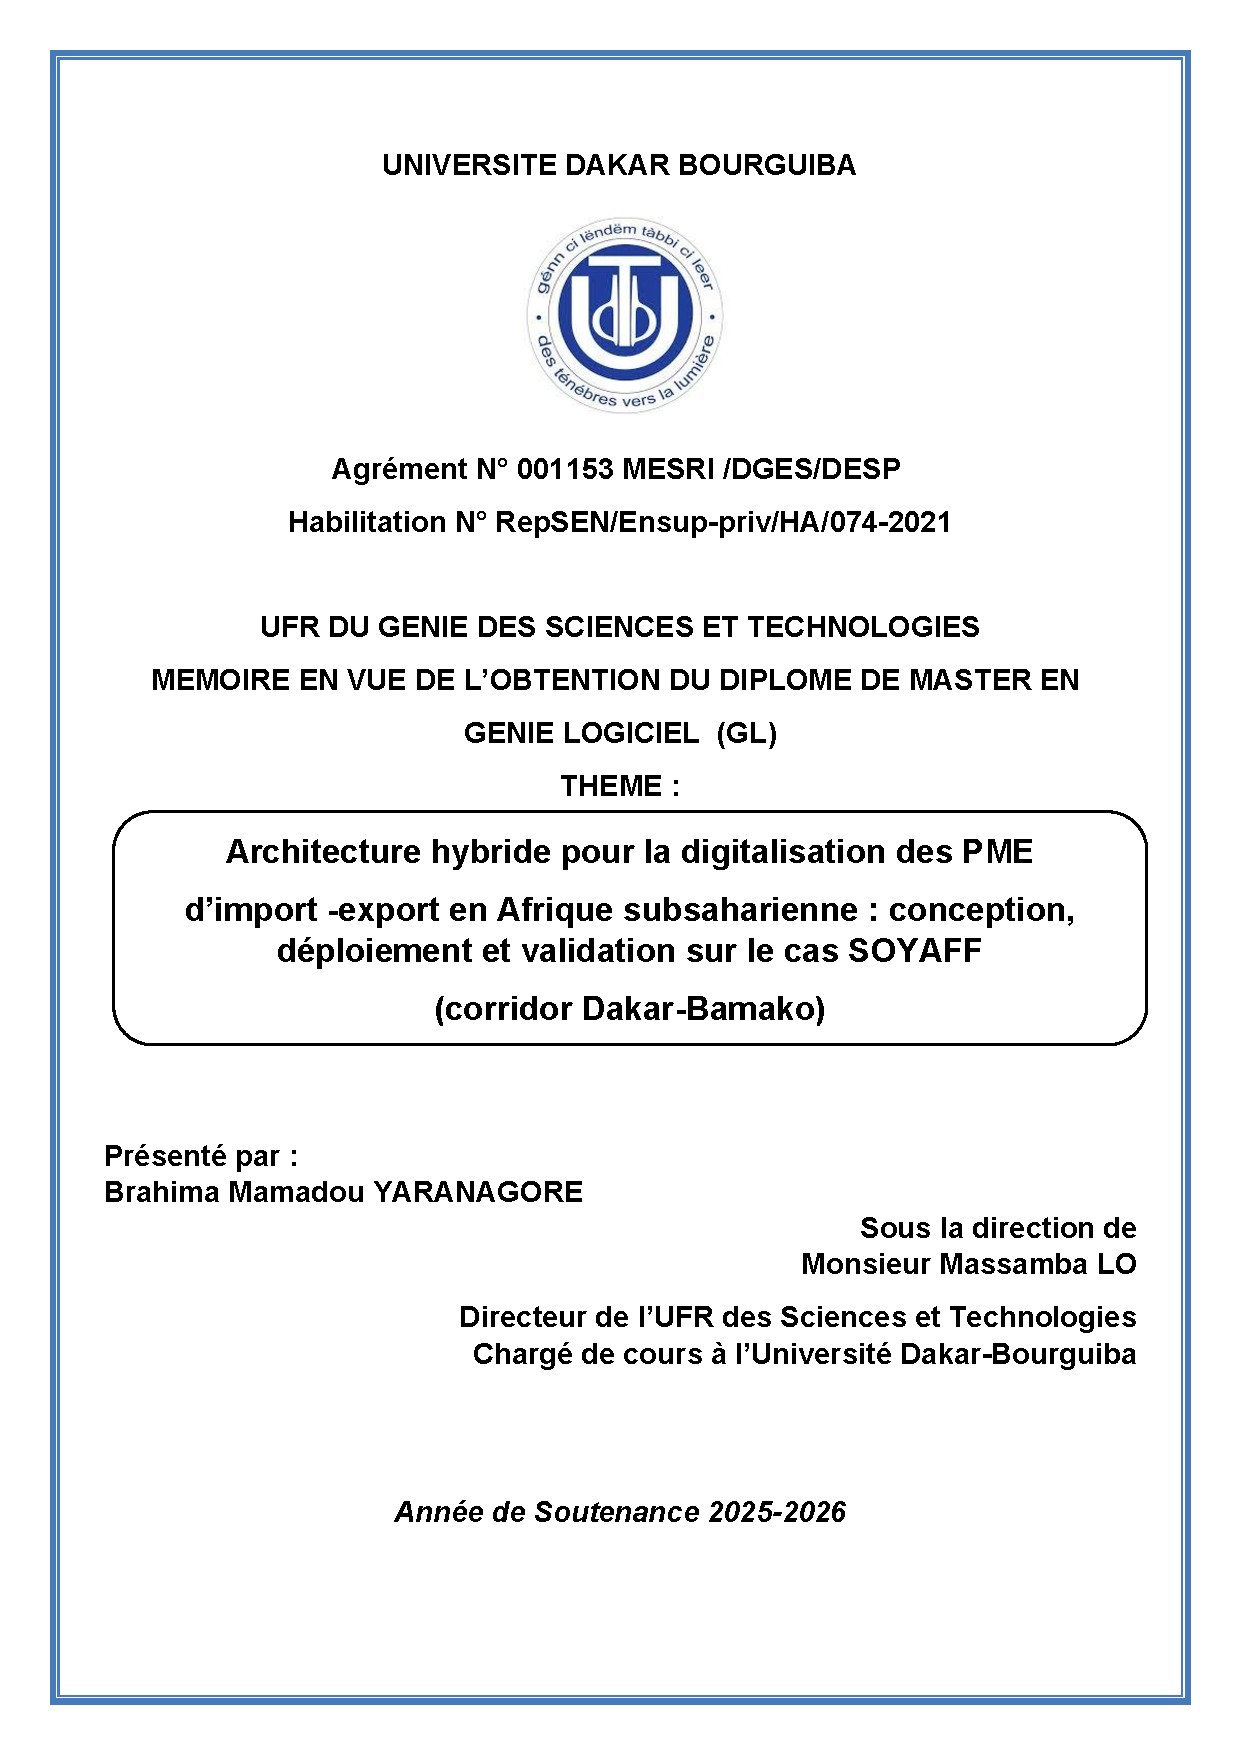
\includepdf[pages=-,noautoscale=true,pagecommand={\thispagestyle{empty}}]{page_de_garde}
\endgroup

% ===== PIÈCES LIMINAIRES (numérotation en chiffres romains, à partir de i) =====
\pagenumbering{roman}
\chapter*{Dédicaces}
\addcontentsline{toc}{chapter}{Dédicaces}

\vspace*{3cm}
\begin{flushright}
\begin{minipage}{0.75\textwidth}
\itshape
Je dédie ce mémoire à mon père, Mamadou Yaranagoré.

Qu'Allah lui fasse miséricorde et lui accorde Son vaste paradis.

Papa, tu aurais tout donné pour voir ce jour. Tu n'es plus là, mais je l'ai fait pour toi.
\end{minipage}
\end{flushright}

\chapter*{Remerciements}
\addcontentsline{toc}{chapter}{Remerciements}

\textit{Al-hamdu lillahi Rabbil-'alamin} : louange à Allah, le Seigneur de l'univers, qui m'a donné la patience, la foi et le courage de mener ce travail à son terme.

Je remercie Monsieur Massamba LO, mon directeur de mémoire, pour sa disponibilité, son sens du partage et son aide tout au long de cette année académique, à mes camarades comme à moi.

Je remercie l'Université Dakar Bourguiba et l'ensemble de son corps professoral pour la formation reçue au cours de ce master.

Je remercie mes collègues de SOYAFF, à Dakar comme à Bamako, qui ont accepté d'utiliser la plateforme, de répondre à mes questions et de me dire franchement ce qui leur manquait. Ce travail leur doit beaucoup.

Je remercie mes camarades de l'UDB pour les échanges et l'entraide pendant ces deux années.

Enfin, je remercie ma famille et mes amis pour leur soutien et leur patience.

% --- RÉSUMÉ ET ABSTRACT (sans numérotation) ---
\chapter*{Résumé}
\addcontentsline{toc}{chapter}{Résumé}
\label{chap:resume}

Les PME représentent plus de 80~\% du tissu économique ouest-africain, mais leur digitalisation reste freinée par des budgets limités, une connexion instable et la crainte de confier leurs données à un tiers. Ce mémoire conçoit, déploie et évalue une architecture hybride pour une PME d'import-export du corridor Dakar--Bamako, SOYAFF. La plateforme comprend un pipeline ETL qui importe seize mois de fichiers Excel, une application web de saisie et de pilotage, et un assistant conversationnel. Chaque question posée à l'assistant est routée selon sa sensibilité : les questions sensibles restent sur le serveur (Mistral~7B), les questions d'analyse partent vers un modèle cloud.

La plateforme tourne en production sur un seul serveur, pour 37,4~€ par mois. Ce coût répond à une réalité de terrain : une PME ouest-africaine n'est pas prête à payer lourdement pour sa digitalisation, quitte à rester sur Excel. Le temps de saisie d'une opération baisse d'environ 85~\%. En valorisant le temps libéré, l'investissement est amorti en 8,5 à 24 mois selon le scénario retenu.

Le chemin local ne répond juste qu'à 20~\% des questions, contre 88,9~\% pour le cloud. Ce résultat apporte l'enseignement principal du travail : la recherche par similarité sémantique est inadaptée à des données relationnelles interrogées par des questions d'agrégat. La suite proposée est un agent \textit{text-to-SQL} exécuté sur le serveur.

\medskip
\noindent\textbf{Mots-clés :} digitalisation des PME, Afrique de l'Ouest, architecture hybride, RAG, \textit{text-to-SQL}, souveraineté des données, ETL.

\chapter*{Abstract}
\addcontentsline{toc}{chapter}{Abstract}
\label{chap:abstract}

Small and medium-sized enterprises (SMEs) make up more than 80\% of the West African economy, but their digital transformation is slowed by small budgets, unstable internet access and the fear of giving their data to a third party. This thesis designs, deploys and evaluates a hybrid architecture for SOYAFF, an import-export SME working on the Dakar--Bamako corridor. The platform includes an ETL pipeline that imports sixteen months of Excel files, a web application for data entry and monitoring, and a conversational assistant. Each question sent to the assistant is routed according to its sensitivity: sensitive questions stay on the server (Mistral~7B), analysis questions go to a cloud model.

The platform runs in production on a single server, for \texteuro{}37.4 per month. This cost matches the reality of the field: a West African SME is not willing to pay heavily for its digital transformation, even if it means staying on Excel. The time needed to enter one operation drops by about 85\%. When the saved time is given a value, the investment pays for itself in 8.5 to 24 months, depending on the scenario.

The local path gives the right answer to only 20\% of the questions, against 88.9\% for the cloud. This result is the main lesson of the work: semantic similarity search is not suited to relational data queried with aggregation questions. The proposed next step is a text-to-SQL agent running on the server.

\medskip
\noindent\textbf{Keywords:} SME digital transformation, West Africa, hybrid architecture, RAG, text-to-SQL, data sovereignty, ETL.


\shorttoc{Sommaire}{0} % parties et chapitres ; table détaillée en fin de document
\listoffigures
\listoftables
% --- GLOSSAIRE ET LISTE DES ACRONYMES (sans numérotation) ---
\chapter*{Liste des acronymes}
\addcontentsline{toc}{chapter}{Liste des acronymes}
\label{chap:acronymes}

\begin{description}
    \item[ADR] Architecture Decision Record, fiche de décision architecturale.
    \item[API] Application Programming Interface, interface de programmation.
    \item[C4] Context, Container, Component, Code, modèle de modélisation architecturale à quatre niveaux.
    \item[CDP] Commission de protection des Données Personnelles (Sénégal).
    \item[CEDEAO] Communauté Économique des États de l'Afrique de l'Ouest.
    \item[CI/CD] Continuous Integration / Continuous Deployment, intégration et déploiement continus.
    \item[CMTR] Conseil Malien des Transporteurs Routiers.
    \item[COSEC] Conseil Sénégalais des Chargeurs.
    \item[CRUD] Create, Read, Update, Delete, opérations élémentaires de persistance.
    \item[CSV] Comma-Separated Values, format de fichier tabulaire.
    \item[DAG] Directed Acyclic Graph, graphe orienté acyclique (unité d'orchestration Airflow).
    \item[EF] Exigence Fonctionnelle.
    \item[ENF] Exigence Non Fonctionnelle.
    \item[ERP] Enterprise Resource Planning, progiciel de gestion intégré.
    \item[ETL] Extract, Transform, Load, extraction, transformation, chargement.
    \item[FCFA] Franc de la Communauté Financière Africaine.
    \item[IA] Intelligence Artificielle.
    \item[JWT] JSON Web Token, jeton d'authentification signé.
    \item[LLM] Large Language Model, grand modèle de langage.
    \item[MoSCoW] Must have, Should have, Could have, Won't have, méthode de priorisation des exigences.
    \item[ODD] Objectifs de Développement Durable.
    \item[OPA] Observatoire des Pratiques Anormales (UEMOA).
    \item[PME] Petite et Moyenne Entreprise.
    \item[RAG] Retrieval-Augmented Generation, génération augmentée par récupération.
    \item[RBAC] Role-Based Access Control, contrôle d'accès à base de rôles.
    \item[ROI] Return On Investment, retour sur investissement.
    \item[SPA] Single Page Application, application web à page unique.
    \item[SPL] Software Product Line, ligne de produits logiciels.
    \item[SQL] Structured Query Language, langage d'interrogation de bases de données relationnelles.
    \item[SUS] System Usability Scale, questionnaire standardisé d'utilisabilité perçue.
    \item[TAM] Technology Acceptance Model, modèle d'acceptation de la technologie.
    \item[TLS] Transport Layer Security, protocole de chiffrement des communications.
    \item[UEMOA] Union Économique et Monétaire Ouest-Africaine.
    \item[UML] Unified Modeling Language, langage de modélisation unifié.
    \item[USD] United States Dollar, dollar américain.
    \item[UTAUT] Unified Theory of Acceptance and Use of Technology, théorie unifiée de l'acceptation et de l'utilisation de la technologie.
\end{description}

\chapter*{Glossaire}
\addcontentsline{toc}{chapter}{Glossaire}
\label{chap:glossaire}

\begin{description}
    \item[Corridor Dakar--Bamako] Axe logistique routier d'environ 1~400~km reliant le port de Dakar à Bamako, colonne vertébrale du commerce extérieur malien.
    \item[Embedding] Représentation vectorielle dense d'un texte, permettant d'en comparer le sens par similarité géométrique plutôt que par correspondance de mots-clés.
    \item[Feature model (modèle de caractéristiques)] Représentation arborescente des caractéristiques communes (invariants) et variables (points de variation) d'une ligne de produits logiciels.
    \item[Frugalité (architecture frugale)] Conception logicielle et d'infrastructure minimisant le coût et les ressources consommées, sous une contrainte budgétaire forte et assumée dès la conception.
    \item[Idempotence] Propriété d'une opération qui, répétée sur les mêmes données, produit le même résultat qu'une seule exécution, ici, rejouer le pipeline ETL n'insère jamais de doublon.
    \item[pgvector] Extension de PostgreSQL ajoutant un type de donnée vectoriel et des opérateurs de recherche par similarité, utilisée pour le retrieval du RAG local.
    \item[Point de variation] Endroit de l'architecture où la variabilité entre membres d'une ligne de produits se manifeste et doit être résolu par une configuration ou un choix propre à chaque instance.
    \item[RAG (Retrieval-Augmented Generation)] Technique augmentant un grand modèle de langage par la récupération préalable de passages ou de données pertinentes, avant génération de la réponse.
    \item[Souveraineté des données] Garantie qu'une donnée ne quitte pas une infrastructure maîtrisée ni la juridiction dont elle relève, notamment vis-à-vis d'un service tiers hébergé à l'étranger.
    \item[Text-to-SQL] Technique par laquelle un modèle de langage traduit une question posée en langage naturel en une requête SQL, exécutée ensuite sur la base de données.
\end{description}

\clearpage

% Mémorise la dernière page romaine des pièces liminaires, pour reprendre
% exactement à cette valeur après la bibliographie (évite un chiffre codé
% en dur qui se décale à chaque modification du contenu liminaire).
\newcounter{derniere_page_romaine}
\setcounter{derniere_page_romaine}{\value{page}}

% ===== CORPS DU MÉMOIRE (numérotation en chiffres arabes, reprise à 1) =====
\pagenumbering{arabic}

% ===== INTRODUCTION =====
% --- INTRODUCTION (sans numérotation) ---
\chapter*{Introduction}
\addcontentsline{toc}{chapter}{Introduction}

\section*{Contexte et motivation}
\label{sec:contexte}

SOYAFF est une entreprise malienne qui a son siège à Bamako, elle a une filiale à Dakar qui gère toute la logistique sur le territoire du Sénégal. En étant employé de l'entreprise comme informaticien au bureau de Dakar j'ai remarqué qu'elle avait un vrai souci de digitalisation car l'entreprise s'appuyait sur des fichiers Excel pour gérer ses opérations logistiques. Le bureau de Dakar a un agent de saisie qui saisit les opérations quotidiennes sur des fichiers Excel appelés \og RECAP-JOURNALIER \fg{} et ces récap-journaliers sont envoyés par WhatsApp sous 24~h normalement. J'ai observé qu'il pouvait y avoir des retards car l'envoi des fichiers sous 24~h était conditionné aux journées types, c'est-à-dire les journées où il peut y avoir 30 à 50 opérations, les journées dites non types comptent peu d'opérations. L'agent attendait alors plusieurs jours pour avoir plus d'opérations et cela pouvait prendre de 48 à 72~h avant d'être envoyé. Cela favorisait la double saisie car le chef logistique résidant à Bamako attend ces informations pour les ressaisir dans sa base de données, il fait ses analyses, consolide et envoie à la comptabilité générale. La lenteur de l'information était aussi un vrai problème car les décideurs n'avaient aucune visibilité en temps réel sur les opérations.

Quand j’avais un projet à rendre pour le module introduction à l’IA avec mon binôme, M. Idrissa Diallo, nous avons décidé de créer un assistant IA pour SOYAFF comme j’avais accès aux données de l’entreprise, après ce projet les données qui étaient autrefois dans des fichiers Excel se retrouvaient dans une base de données relationnelle et vectorielle avec PostgreSQL et pgvector, je me suis dit que je vais pallier ce problème en concevant une application Web fullstack pour la gestion des opérations de SOYAFF. J’ai présenté le MVP au chef logistique. Il était d’accord avec moi pour continuer sur le projet mais il y avait certaines préoccupations qui étaient : il craignait la sécurité de l’application, il ne voulait pas que nos données partent chez un tiers car elles contenaient des données personnelles et monétaires, d’où mon idée de faire coexister deux approches d’IA Cloud avec Claude pour sa capacité de raisonnement pour les requêtes complexes et non sensibles et l’autre locale Ollama/Mistral pour les requêtes sensibles contenant des données personnelles.

Mon travail s'inscrit dans le sens où je veux aider SOYAFF à augmenter sa productivité car selon un article de blog de F. Bandia~\cite{fatimaAfriqueLOuestPME}, les PME représentent plus de 80~\% du tissu économique de la plupart des pays africains, seules 23~\% des PME ouest-africaines ont réellement intégré le numérique alors que celles qui passent ce cap enregistrent une hausse en moyenne d'environ 32~\%. Je me devais ainsi de concevoir une application basée sur les réalités géographiques des pays ouest-africains, car ces pays souffrent du manque de haut débit de connectivité dû à la fracture territoriale et l'exposition aux ruptures de câbles sous-marins \cite{cariolleInfrastructuresEconomieNumeriques2018}. Et le cas SOYAFF n'est pas un cas isolé quand on sait que jusqu'à 80~\% du commerce du Mali, pays enclavé, transite par le corridor Dakar--Bamako \cite{byiersActeursInteretsLong2022}.

\section*{Contexte spécifique du projet SOYAFF}
\label{sec:contexte_soyaff}

SOYAFF produit et importe des produits de première nécessité, et exporte aussi ses propres produits. Le bureau de Dakar gère au quotidien le suivi et les plans de chargement des camions, les contraventions, les rations des chauffeurs qui restent plus de cinq jours au Sénégal, les primes de liaison, les frais mécaniques et les achats de pièces. Tout ça sur Excel ou à la main, ça ralentissait l'entreprise et ça nuisait à la prise de décision. D'où la nécessité de digitaliser ces opérations.

Notre travail préliminaire a abouti à la mise en place d'une première plateforme de gestion logistique, déjà déployée en production sur le domaine \url{soyaff-logstique.com} (orthographe exacte du domaine), qui intègre un pipeline ETL traitant 16 mois de données réelles (4~755 transactions, 319 camions) et une base PostgreSQL (\texttt{pgvector}).

On qualifie notre architecture d'\textbf{hybride} parce qu'elle fait coexister deux façons de traiter les requêtes par IA générative : un service cloud, l'API propriétaire de Claude (Anthropic), pour les requêtes complexes qui demandent une bonne capacité de raisonnement, et un service local auto-hébergé, Mistral via Ollama, pour les requêtes sensibles qui doivent rester sous le contrôle de l'entreprise.

\section*{Problématique}
\label{sec:problematique}

Le cas SOYAFF, et plus généralement celui des PME d'import-export ouest-africaines, soulève la question suivante :

\begin{quote}
    \textbf{Comment concevoir, déployer et valider une architecture logicielle hybride et réplicable pour digitaliser les processus opérationnels d'une PME d'import-export ouest-africaine ? L'architecture doit intégrer un pipeline ETL automatisé et une IA générative souveraine pour l'aide à la décision, tourner sur une infrastructure DevOps solide, et tenir compte des contraintes du terrain : budget serré, connectivité limitée, souveraineté des données.}
\end{quote}

\section*{Questions de recherche}
\label{sec:questions_recherche}

Cette problématique se décompose en quatre questions de recherche structurées comme suit :
\begin{itemize}
    \item \textbf{Q1}~: Quelle architecture logicielle adopter pour digitaliser un processus logistique transfrontalier, avec une connectivité limitée et un budget contraint, dans une PME ouest-africaine ?
    \item \textbf{Q2}~: Un système RAG cloud (API Claude Anthropic) donne-t-il des résultats comparables à un système RAG auto-hébergé (Ollama/Mistral) sur un corpus métier en langue française ? Je compare leur performance, leur exactitude, leur coût et leur niveau de souveraineté des données.
    \item \textbf{Q3}~: Comment mesurer l'impact métier et le coût réel d'une digitalisation assistée par IA dans une PME logistique africaine ? Je regarde le temps gagné, les erreurs évitées, le coût et l'adoption par les utilisateurs.
    \item \textbf{Q4}~: L'architecture conçue pour SOYAFF est-elle généralisable à d'autres PME d'import-export d'Afrique subsaharienne ? Et si oui, qu'est-ce qui reste stable d'un cas à l'autre, et qu'est-ce qu'il faut reconfigurer ?
\end{itemize}

\section*{Hypothèses scientifiques}
\label{sec:hypotheses}

Afin de répondre à ces interrogations, quatre hypothèses scientifiques sont posées et seront mises à l'épreuve par les expérimentations conduites dans la suite de ce travail :

\begin{itemize}
    \item \textbf{H1 (coût maîtrisé)}~: L'architecture complète (pipeline ETL, application web full-stack, IA générative) peut tourner et être maintenue pour moins de 50~€/mois, un coût à la portée d'une PME africaine.
    \item \textbf{H2 (le RAG local tient la comparaison)}~: Sur un corpus métier restreint et bien défini, le RAG auto-hébergé atteint une exactitude comparable au RAG cloud (à 90~\% près), tout en gardant les données sous le contrôle total de l'entreprise.
    \item \textbf{H3 (moins de saisie, moins d'erreurs)}~: Supprimer la double saisie entre les sites distants réduit le temps de traitement journalier des opérations d'au moins 70~\% et le taux d'erreur de saisie d'au moins 80~\%.
    \item \textbf{H4 (ça se réplique ailleurs)}~: L'architecture a un noyau d'invariants assez stables et des points de variation identifiables pour être reprise par d'autres PME d'import-export en Afrique subsaharienne, sans refonte structurelle majeure.
\end{itemize}

\section*{Contributions attendues}
\label{sec:contributions}

Ce travail devrait apporter quatre choses :
\begin{enumerate}
    \item \textbf{Une plateforme} livrée et opérationnelle en production réelle chez SOYAFF, documentée et maintenue sous gestion de version.
    \item \textbf{Une étude comparative}, sur un terrain africain encore peu documenté, entre un RAG cloud et un RAG local sur un corpus métier en langue française.
    \item \textbf{Un cadre d'évaluation} à trois dimensions (technique, métier, adoption), pensé pour mesurer l'impact d'une digitalisation dans une PME africaine.
    \item \textbf{Un référentiel d'architecture} réplicable, construit sur une analyse par lignes de produits logiciels, pour faciliter la digitalisation d'autres PME du même secteur.
\end{enumerate}

\section*{Plan du mémoire}
\label{sec:plan_memoire}

Le mémoire compte trois parties et six chapitres.

\textbf{La Partie I} pose le cadre théorique et méthodologique. Le chapitre~\ref{chap:contexte} décrit le corridor Dakar--Bamako et la société SOYAFF, pose le diagnostic de son système d'information, puis fixe les objectifs (\S\ref{sec:objectifs}) et la méthodologie (\S\ref{sec:methodologie}).

\textbf{La Partie II} forme le cadre conceptuel. Le chapitre~\ref{chap:etat_art} passe en revue la littérature sur la digitalisation des PME africaines, les architectures ETL, les systèmes RAG et la souveraineté numérique. Le chapitre~\ref{chap:conception} en tire la conception : analyse des besoins, modélisation UML et architecture C4, chaque choix critique étant justifié par un \textit{Architecture Decision Record}.

\textbf{La Partie III} porte la mise en œuvre. Le chapitre~\ref{chap:realisation} décrit la réalisation : pipeline ETL sous Airflow, application web, module d'IA hybride, infrastructure DevOps. Le chapitre~\ref{chap:evaluation} évalue la plateforme : test de bout en bout, benchmark RAG, impact métier, adoption, généralisation, retour sur investissement. Le chapitre~\ref{chap:discussion_perspectives} discute les résultats et trace les perspectives, dont une plateforme SaaS multi-tenant.

Une conclusion referme le mémoire en reprenant les questions de recherche et en synthétisant les apports.

%   FIN DE L'INTRODUCTION ---

% ===== PARTIE I : CADRE THÉORIQUE ET MÉTHODOLOGIQUE =====
\part{Cadre théorique et méthodologique}

\chapter{Contexte de l'étude}
\label{chap:contexte}

\section{Le corridor Dakar–Bamako : enjeux logistiques et économiques}
\label{sec:corridor}

\subsection{Géographie et importance stratégique du corridor}
Le Mali se caractérise par sa situation géographique de pays enclavé, dépourvu de tout accès direct à la mer. Cette configuration structurelle impose à son économie une dépendance critique vis-à-vis des infrastructures de transport des pays côtiers de la zone ouest-africaine. Dans ce contexte, le Port Autonome de Dakar s'impose comme le principal débouché et la porte d’accès maritime naturelle pour les flux d'importation et d'exportation maliens. 

Le corridor routier reliant Dakar à Bamako se déploie sur une distance d'environ 1~400 kilomètres. Cet axe représente une artère vitale par laquelle transite jusqu'à 80 \% du commerce global du Mali. L'approvisionnement en produits de première nécessité ainsi que l'acheminement des intrants industriels et agricoles reposent de manière prépondérante sur la continuité opérationnelle de cet axe géoéconomique majeur, comme le soulignent les travaux de Byiers et Rosengren \cite{byiersActeursInteretsLong2022} (cf. figure~\ref{fig:corridor_dakar_bamako}).
\begin{figure}[H]
  \centering
  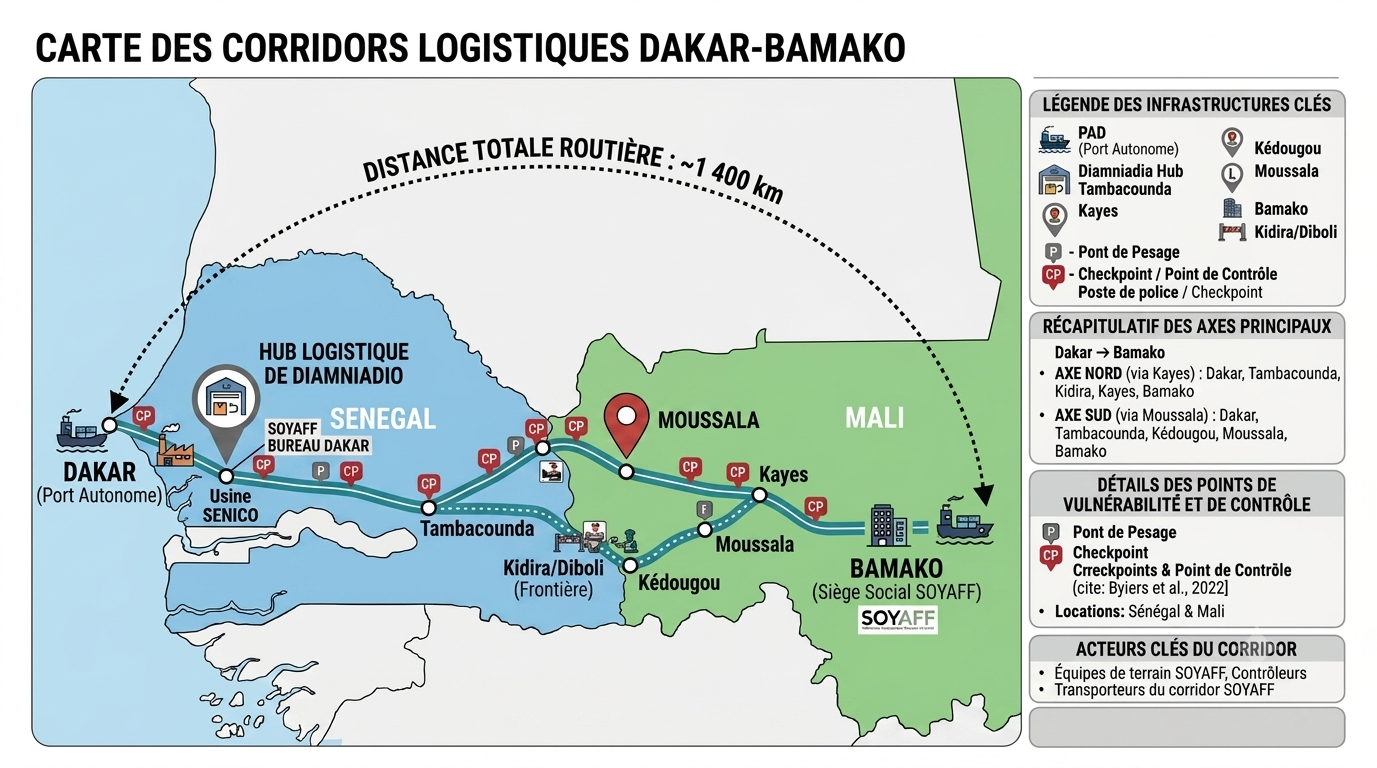
\includegraphics[width=0.95\textwidth]{figure_1_1_corridor}
  \caption{Corridor logistique Dakar--Bamako : axes routiers, ponts de
           pesage (Afrique Pesage S.A.) et checkpoints officiels et
           frontaliers (Kidira/Diboli pour l'axe nord, Moussala pour l'axe sud).}
  \source{Schéma illustratif de l'auteur, d'après Kébé et al.
          \cite{fix_kebeDiagnosticEntravesImportance2023}, Sigué \cite{sigueTransportRoutierMarchandises2017}, Byiers et Rosengren
          \cite{byiersActeursInteretsLong2022} et UEMOA/OPA \cite{uemoaOPA2017}}
  \label{fig:corridor_dakar_bamako}
\end{figure}

\subsection{Les acteurs clés de la chaîne logistique}
L'exploitation et la régulation de ce corridor font intervenir une multitude d'acteurs institutionnels et privés dont la coordination est essentielle. Au premier plan figurent les transporteurs routiers, segment composé de grands opérateurs logistiques mais également d'un tissu dense de Petites et Moyennes Entreprises (PME) nationales. Sur le plan régalien, l'administration des douanes sénégalaises et l'administration des douanes maliennes contrôlent la conformité des marchandises aux frontières. 

Les principaux points de passage frontaliers se concentrent au niveau de l'axe Kidira, du côté sénégalais, et de Diboli, du côté malien. Les Conseils nationaux des chargeurs, à savoir le Conseil Sénégalais des Chargeurs (COSEC) et le Conseil Malien des Transporteurs Routiers (CMTR), interviennent pour défendre les intérêts des opérateurs et faciliter les procédures. Bien que ces interactions s'inscrivent théoriquement dans les cadres communautaires de l'UEMOA et de la CEDEAO prônant la libre circulation des biens, l'application concrète de ces accords se heurte régulièrement à des freins administratifs et opérationnels majeurs.

Un acteur supplémentaire structure de façon déterminante le quotidien des transporteurs sur cet axe : le contrôle du gabarit, du poids et de la charge à l'essieu des poids lourds, encadré par le Règlement n\textsuperscript{o}14/2005/CM/UEMOA \cite{REGLEMENTNdeg142005}. Ce texte communautaire fixe des limites strictes que tout véhicule circulant sur le réseau routier des États membres doit respecter, qu'il s'agisse de la charge maximale autorisée à l'essieu (CMAE), du poids total autorisé en charge (PTAC) ou du poids total roulant autorisé (PTRA) pour les ensembles articulés. Au Sénégal, le contrôle de cette réglementation sur le réseau routier national a été délégué à un concessionnaire dédié, dont les stations fixes et mobiles sont notamment implantées sur les axes stratégiques de Mbour, Kaffrine, Tambacounda et Kidira, points de passage obligés pour les flux internationaux à destination du Mali. Pour les ensembles routiers internationaux tels que ceux exploités par SOYAFF, le respect simultané de ces deux contraintes (répartition correcte de la charge par essieu et plafond global du poids roulant) conditionne directement la fluidité du passage aux points de contrôle et constitue une source additionnelle de risque opérationnel (immobilisation, amende, délestage) en cas de non-conformité.

Pour rationaliser les contrôles routiers et accélérer le passage des corridors, l'État du Sénégal a adopté le décret n\textsuperscript{o}2021-1600 du 3 décembre 2021, complété par un arrêté interministériel instituant des brigades mixtes de contrôle routier (Gendarmerie, Police) et limitant en principe à trois le total des points de contrôle officiels par corridor national \cite{ControlesRoutiersAu2026}. Cette limitation théorique s'inscrit dans la lignée des recommandations communautaires de l'UEMOA, qui préconise également un plafond de trois postes de contrôle par corridor (au départ, au poste juxtaposé frontalier, et à destination). Dans la pratique cependant, la quantité de points de contrôle effectivement constatés sur le terrain dépasse régulièrement cette norme communautaire, comme le documentent les rapports périodiques de l'Observatoire des Pratiques Anormales (OPA) de l'UEMOA (cf. §1.1.3).

Une partie de ce dispositif de contrôle physique tend à être progressivement complétée, voire substituée, par des dispositifs de géolocalisation embarqués. D'après l'observation directe que nous avons conduite chez SOYAFF, une fraction significative de la flotte de camions de la société est équipée de balises de tracking GPS sur le territoire sénégalais, ce qui réduit dans certains cas la nécessité d'un contrôle physique systématique par les agents au profit d'un suivi à distance. Cette évolution, bien que partielle et non généralisée à l'ensemble du corridor, illustre une tendance plus large à la numérisation du contrôle logistique et renforce la pertinence d'une architecture capable d'exploiter de telles données de géolocalisation pour le suivi de flotte.

\subsection{Contraintes opérationnelles et vulnérabilités numériques}
L'efficacité du corridor Dakar--Bamako est lourdement grevée par la persistance de barrières non tarifaires, en dépit du cadre réglementaire théoriquement restrictif évoqué en §1.1.2. Si la norme communautaire de l'UEMOA et le décret sénégalais n\textsuperscript{o}2021-1600 fixent à trois le plafond de points de contrôle officiels par corridor, les rapports périodiques de l'OPA (initiative mise en place dès 2005 avec l'appui de l'USAID pour suivre la gouvernance routière dans l'espace communautaire) font régulièrement état d'un nombre de contrôles effectivement constatés sur le terrain bien supérieur à cette norme, ainsi que de prélèvements illicites persistants \cite{uemoaOPA2017}. Le corridor Dakar--Bamako figure parmi les axes où les temps de contrôle aux postes frontaliers sont les plus élevés de l'espace UEMOA, l'OPA ayant mesuré des temps moyens de l'ordre de 147 à 154 minutes selon le point de passage frontalier emprunté (Diboli ou Moussala) \cite{uemoaOPA2017}.

Cet écart entre le cadre réglementaire et la pratique observée engendre des retards systémiques et une inflation artificielle des coûts logistiques globaux. Les délais de transit s'avèrent de ce fait extrêmement variables, oscillant généralement entre 3 et 7 jours selon les conditions de circulation, les formalités douanières et les aléas administratifs. À ces frictions physiques s'ajoutent des enjeux de sécurité sur certains tronçons de l'itinéraire, obligeant les transporteurs à une vigilance accrue. 

Enfin, le corridor fait face à des vulnérabilités numériques notables. Conformément aux analyses de Cariolle \cite{cariolleInfrastructuresEconomieNumeriques2018}, les infrastructures de communication subissent des instabilités chroniques, allant des ruptures accidentelles de câbles sous-marins à une fracture numérique territoriale marquée entre les grands centres urbains et les zones frontalières enclavées.

\subsection{Les défis de gestion pour les PME de transport}
Pour les PME de transport routier, l'ensemble de ces contraintes se traduit par un manque aigu de visibilité sur la flotte en transit. Les difficultés de coordination asynchrone entre la plateforme de départ à Dakar et le siège décisionnel situé à Bamako nuisent à la productivité globale. En l’absence d'outils de suivi interconnectés, le pilotage en temps réel des camions devient impossible, laissant les gestionnaires désarmés face aux imprévus du corridor. C'est dans ce contexte que la société SOYAFF exerce son activité.

\section{La société SOYAFF : organisation et processus opérationnels}
\label{sec:soyaff_orga}

\subsection{Identification et activité de la société}
La société SOYAFF est une Petite et Moyenne Entreprise (PME) spécialisée dans la logistique et le commerce d'import-export, axée principalement sur la production, l'importation et la distribution de produits de première nécessité entre le Mali et le Sénégal. Pour soutenir cette activité transfrontalière et s'adapter aux configurations géographiques de la sous-région, la société dispose d'un siège social stratégique établi à Bamako (Mali) et d'une succursale opérationnelle implantée à Dakar (Sénégal). 

L'importance de son activité se reflète à travers la volumétrie substantielle enregistrée lors de notre travail de terrain : sur une fenêtre d'observation de 16 mois, SOYAFF a traité un total de 4~755 transactions, mobilisant 319 camions et générant 727 bons de chargement.

\begin{small}
\textit{L'utilisation des données opérationnelles de SOYAFF dans le cadre du présent travail a été formellement autorisée par la direction de la société, sous réserve d'anonymisation des informations financières et personnelles sensibles.}
\end{small}

\subsection{Structure organisationnelle et acteurs clés}
L'organisation humaine de SOYAFF repose sur une répartition géographique rigoureuse des rôles, nécessaire pour piloter un flux de marchandises s'étendant sur 1~400 kilomètres :
\begin{itemize}
    \item \textbf{À Bamako (Siège)} : Le chef logistique centralise les besoins du marché malien, planifie les grandes orientations de la flotte et attend les consolidations manuelles de données pour effectuer le reporting global destiné à la direction.
    \item \textbf{À Dakar (Succursale)} : L'équipe comprend un chef de bureau, un assistant principal et des agents de saisie chargés de consigner manuellement sur tableur les événements quotidiens liés à l'affrètement et au chargement des camions au départ du Port Autonome de Dakar.
    \item \textbf{Sur le corridor} : Une flotte de 45 chauffeurs actifs assure les liaisons de transport. La hiérarchie de validation des dépenses et des incidents suit un circuit strict allant du chauffeur vers l'assistant principal pour un premier visa, avant validation finale par le chef de bureau de Dakar.
\end{itemize}

\subsection{Cartographie des processus opérationnels quotidiens}
L'activité quotidienne génère un volume important de flux d'informations et de documents physiques. Le tableau \ref{tab:processus_soyaff} synthétise la nature, la fréquence et la volumétrie de ces processus que nous avons observés.

\begin{table}[htbp]
\centering
\caption{Synthèse des processus opérationnels et volumétries chez SOYAFF}
\label{tab:processus_soyaff}
\begin{tabular}{|>{\raggedright\arraybackslash}p{4.3cm}|>{\raggedright\arraybackslash}p{2.4cm}|>{\raggedright\arraybackslash}p{2.6cm}|>{\raggedright\arraybackslash}p{3.4cm}|}
\hline
\textbf{Processus} & \textbf{Fréquence} & \textbf{Volume estimé} & \textbf{Support actuel} \\ \hline
Plans de chargement camions & Quotidien & 5 à 10 / jour & Fiches papier + Excel \\ \hline
Gestion des contraventions & Variable & 2 à 8 / semaine & Excel + reçus papier \\ \hline
Rations chauffeurs (séjour > 5j) & Hebdomadaire & $\sim$15 / semaine & Fiches \texttt{AUT-DEP} papier \\ \hline
Primes de liaison & À chaque liaison & $\sim$25 / mois & Excel + reçus \\ \hline
Frais mécaniques et pièces & Variable & $\sim$30 / mois & Factures papier + Excel \\ \hline
Récapitulatif journalier & Quotidien & 1 / jour & Fichier Excel \\ \hline
Récapitulatif mensuel & Mensuel & 1 / mois & Excel consolidé \\ \hline
\end{tabular}
\end{table}

\subsection{Outils technologiques en usage}
Le système d’information actuel de la société SOYAFF se caractérise par une absence totale de base de données centralisée ou de progiciel de gestion intégré (ERP). Les outils se limitent à l'utilisation de fichiers de tableurs décentralisés, principalement dénommés \texttt{RECAP-JOURNALIERE} et \texttt{RECAP-MENSUEL}. Les autorisations de dépenses et le suivi des frais s'appuient sur des fiches physiques au format papier, appelées fiches \texttt{AUT-DEP} (Autorisation de Dépense). Les flux de communication formels s'effectuent par courrier électronique, tandis que la coordination informelle et instantanée des urgences sur le corridor (pannes, blocages aux checkpoints) repose sur l'application grand public WhatsApp. Une application mobile tierce, \texttt{kiri.app}, est aussi en usage, mais son périmètre se limite strictement à la conformité administrative (collecte des pièces signées par les représentants logistiques) : elle ne propose aucun module de suivi de caisse, de tableau de bord ou d'analyse décisionnelle.

\section{Diagnostic du système d'information existant}
\label{sec:diagnostic_si}

\subsection{Flux d'information actuel et rupture de saisie}
Le parcours d'une donnée opérationnelle au sein de SOYAFF met en lumière une rupture flagrante dans la chaîne de traitement de l'information. Lorsqu'un camion est chargé ou qu'un frais est engagé à Dakar, l'agent de saisie local consigne l'information dans son fichier Excel récapitulatif. En fin de journée, ce document \texttt{RECAP-JOURNALIERE} est transmis par e-mail ou via WhatsApp au siège à Bamako. 

À la réception, le chef logistique de Bamako doit ouvrir le fichier et procéder à une \textbf{ressaisie manuelle intégrale}, ligne par ligne, de l'ensemble des transactions dans sa propre base de données locale afin de pouvoir calculer les agrégats de performance. Cette double saisie systématique crée une zone de vulnérabilité majeure : toute erreur ou besoin de clarification impose de longs échanges et des allers-retours correctifs asynchrones par téléphone ou messagerie entre Dakar et Bamako.

\subsection{Analyse ancrée : Les contraintes macro du corridor face au micro-système}
Pour comprendre la fragilité du système d'information de SOYAFF, il faut le confronter aux réalités du corridor routier Dakar–Bamako. Selon les données de l'OPA, ce corridor long de près de 1~400 km subit une moyenne critique de \textbf{31,47 contrôles routiers par voyage} (soit environ 2,13 points de contrôle pour 100 km), générant des perceptions illicites moyennes de 43~078 F~CFA par trajet pour un camion pourtant en règle \cite{fix_kebeDiagnosticEntravesImportance2023}. Ce chiffre confirme, à une échelle plus précise, l'écart déjà constaté en §1.1.3 entre le plafond réglementaire de trois points de contrôle par corridor et la réalité du terrain.

De plus, l'axe détient un temps d'attente cumulé élevé aux points de passage frontaliers, atteignant une moyenne de \textbf{316 minutes de stagnation} par voyage du fait de la lenteur des formalités douanières administratives \cite{sigueTransportRoutierMarchandises2017}. En l'absence d'un système d'information interconnecté, ces événements imprévisibles (perceptions informelles sans reçu officiel, immobilisations prolongées aux gares de rupture de charge) sont gérés de manière totalement opaque par des messages WhatsApp volatils, empêchant la PME d'anticiper la rotation théorique de ses camions, estimée en moyenne à 14 jours sur cet axe \cite{sigueTransportRoutierMarchandises2017}.

\subsection{Typologie des limites observées}
L'analyse critique du système actuel permet de classifier ses faiblesses structurelles en quatre catégories distinctes :
\begin{enumerate}
    \item \textbf{Limites opérationnelles} : La double saisie systématique s'avère extrêmement chronophage, consommant en moyenne 2 à 3 heures de travail quotidien pour le seul chef logistique à Bamako. Ce mode de fonctionnement asynchrone induit une latence d'information de 24 à 48 heures, empêchant toute exploitation immédiate des données opérationnelles du jour J. Enfin, le transfert manuel de fichiers isolés par e-mail expose l'entreprise à des risques élevés de perte de données ou de désynchronisation de versions.
    \item \textbf{Limites qualitatives} : La manipulation humaine répétée de milliers de lignes engendre inévitablement des erreurs de saisie (inversion de dates, fautes de frappe sur les immatriculations ou les montants), des doublons, des omissions et des ruptures fréquentes de formules de calcul au sein des tableurs Excel lors des consolidations mensuelles.
    \item \textbf{Limites décisionnelles} : La direction ne dispose d'aucun tableau de bord mis à jour en temps réel. Il est impossible d'extraire instantanément des analyses avancées, telles que la dérive des coûts de carburant par camion ou les tendances de performance de la flotte face au harcèlement routier. Les décisions managériales sont ainsi guidées par l'intuition et l'expérience empirique plutôt que par des indicateurs factuels fiables.
    \item \textbf{Limites stratégiques} : L'absence d’historique centralisé, sécurisé et structuré au-delà du mois courant bloque toute tentative de planification ou d'analyse prédictive à moyen terme. Ce système bloque la croissance : si la flotte de camions venait à s'agrandir, la structure administrative actuelle s'effondrerait sous le poids des ressaisies manuelles et de l'asynchronisme.
\end{enumerate}

\subsection{Conséquences financières et organisationnelles}
Les impacts de cette dette opérationnelle sont multiples et se déclinent sur trois plans complémentaires.

Sur le plan financier, le coût caché lié au temps passé par des cadres qualifiés à ressaisir des lignes Excel représente une perte économique quantifiable à l'échelle de l'exercice annuel. En prenant pour base les 2 à 3 heures quotidiennes consacrées à la double saisie par le chef logistique de Bamako (cf. §1.3.3), et en valorisant ce temps au coût horaire chargé d'un cadre logistique dans la sous-région, la perte annuelle directement imputable à cette seule tâche redondante peut être estimée à plusieurs centaines d'heures de travail qualifié, soit l'équivalent de plusieurs mois-homme par an. À cela s'ajoute un coût indirect, plus difficile à quantifier mais tout aussi réel : la non-détection en temps réel des taxes informelles (43~078 F~CFA en moyenne par trajet selon les données de l'OPA, cf. §1.3.2) et des failles logistiques grève directement la rentabilité de l'entreprise, sans que la direction dispose des moyens de les anticiper ou de les contester.

Sur le plan organisationnel, la lourdeur des processus engendre une frustration partagée par les équipes et crée une dépendance critique vis-à-vis d'individus clés, détenteurs exclusifs des fichiers tableurs. Cette concentration du savoir opérationnel constitue un facteur de risque significatif : l'absence ou le départ d'un agent de saisie expérimenté peut paralyser temporairement la chaîne de remontée d'information. Face à un corridor en voie de modernisation et d'intégration régionale accélérée (ZLECAf, guichets uniques portuaires), l'absence de transformation numérique expose SOYAFF à un risque majeur de perte de compétitivité face à des concurrents plus agiles.

Enfin, sur le plan stratégique, cette situation prive la direction de SOYAFF d'un levier essentiel de pilotage : sans visibilité fiable sur les coûts réels par trajet, par camion ou par chauffeur, toute décision d'investissement (renouvellement de flotte, ouverture de nouvelles lignes, négociation tarifaire) repose sur des estimations approximatives plutôt que sur des données consolidées.

\section{Synthèse du diagnostic et positionnement du projet}
\label{sec:synthese_diagnostic}

L'analyse conduite dans ce chapitre met en évidence une situation paradoxale, déjà identifiée à l'échelle macro-économique en introduction : alors que le corridor Dakar--Bamako constitue un axe stratégique majeur pour l'économie malienne, et que SOYAFF y occupe une position d'acteur logistique établi traitant plusieurs milliers de transactions sur 16 mois, son système d'information repose encore intégralement sur des outils bureautiques non interconnectés. SOYAFF n'est pas un cas à part : l'entreprise évolue dans un secteur précis, sur un corridor bien déterminé, ce qui la rend représentative des PME d'import-export opérant sur des corridors comparables en Afrique de l'Ouest, où la digitalisation reste largement à faire.

Ce diagnostic oriente la suite du travail. Les dysfonctionnements observés ne viennent pas d'un manque de volonté ou de compétence des équipes, mais d'un outillage inadapté à leur contexte : connexion intermittente, budget serré, deux sites distants de 1~400 kilomètres. Toute solution devra composer avec ces contraintes. La typologie des limites (\S\ref{sec:diagnostic_si}) servira de grille pour structurer les exigences du système (section~\ref{chap:besoins}). Enfin, la nature des données traitées (montants, identités des chauffeurs) fait de la souveraineté une contrainte de conception, et non une option. C'est elle qui justifie une architecture combinant une IA générative cloud et une IA auto-hébergée.

Une solution générique ne suffit donc pas pour SOYAFF. L'entreprise n'est pas prête à investir lourdement dans sa digitalisation, quitte à rester sur Excel ; elle travaille avec une connexion instable ; et son chef logistique refuse que les données partent chez un tiers. L'architecture doit répondre à ces trois réalités.

\section{Objectifs de l'étude}
\label{sec:objectifs}

\textbf{Objectif général (OG).} Concevoir, déployer et évaluer scientifiquement une architecture logicielle hybride et réplicable pour la digitalisation des PME d'import-export en Afrique subsaharienne, en prenant SOYAFF comme cas de validation principal.

\textbf{Objectifs spécifiques (OS).} Pour y parvenir, nous nous sommes fixé les objectifs suivants :
\begin{itemize}
    \item[\textbf{OS1}] \textbf{Documenter} l'état de l'art sur la digitalisation des PME africaines, les architectures ETL, les systèmes RAG et la souveraineté numérique.
    \item[\textbf{OS2}] \textbf{Caractériser} le domaine des PME d'import-export ouest-africaines pour en dégager les invariants et les points de variation.
    \item[\textbf{OS3}] \textbf{Spécifier} l'architecture selon le modèle C4, en justifiant chaque choix par un \textit{Architecture Decision Record} (ADR).
    \item[\textbf{OS4}] \textbf{Mettre en œuvre, déployer et exploiter} la plateforme en production sur le cas SOYAFF.
    \item[\textbf{OS5}] \textbf{Mener} un benchmark comparant le RAG cloud et le RAG local sur 30 questions métier représentatives, puis \textbf{mesurer} l'impact métier et le coût réel de la solution (gain horaire, taux d'erreur, coût mensuel).
    \item[\textbf{OS6}] \textbf{Étudier} l'adoption utilisateur avec le questionnaire \textit{System Usability Scale} (SUS) et des entretiens semi-directifs.
    \item[\textbf{OS7}] \textbf{Analyser} la généralisation de l'architecture avec l'approche des lignes de produits logiciels (\textit{Software Product Lines}), pour distinguer ce qui reste stable de ce qui doit être reconfiguré d'une PME à l'autre.
    \item[\textbf{OS8}] \textbf{Formaliser} un référentiel d'architecture réplicable, utile à la recherche comme à d'autres projets du même type.
\end{itemize}

\section{Méthodologie de recherche}
\label{sec:methodologie}

Pour mener à bien ce projet, nous adoptons une approche entre ingénierie logicielle et évaluation scientifique. Sur le plan de l'ingénierie, nous appliquons une démarche hybride agile, combinant des cycles itératifs avec une formalisation systématique des choix architecturaux via des ADR (\textit{Architecture Decision Records}). La modélisation s'appuie sur le framework C4 (Context, Container, Component, Code), enrichi par les diagrammes UML pertinents. En outre, pour le développement de nouvelles fonctionnalités, nous adoptons une démarche inspirée de Scrum : chaque fonctionnalité fait l'objet d'un ticket Jira classé par priorité dans un sprint, et une branche Git dédiée est créée pour chaque ticket. Le code est hébergé et déployé sur GitLab, où chaque \textit{push} sur la branche principale déclenche automatiquement le pipeline de déploiement (voir section~\ref{chap:devops}).

Côté scientifique, l'évaluation repose sur trois angles. D'abord un benchmark qui compare les deux systèmes RAG sur la latence, l'exactitude et le taux d'hallucination. Ensuite une étude avant/après digitalisation pour chiffrer les gains opérationnels. Et pour l'adoption utilisateur, nous nous appuyons sur le questionnaire \textit{System Usability Scale} (SUS) \cite{brookeSUSAQuickDirty1996} et sur des entretiens semi-directifs.

Le benchmark comparatif constitue le cœur de l'évaluation scientifique. Il repose sur un corpus de 30 questions métier, six par catégorie fonctionnelle : suivi de flotte, gestion financière, analyse des incidents, conformité documentaire et aide à la décision stratégique. Chaque question est aussi classée selon le type de réponse attendue : T1 pour un chiffre ou un fait vérifiable par une requête SQL (15 questions), T2 pour une liste (10 questions), T3 pour une analyse jugée sur grille (5 questions). Les deux systèmes sont interrogés trois fois par question sur le serveur de production. Nous mesurons la latence (P50, P95, P99), l'exactitude par comparaison à une vérité-terrain fixée avant toute exécution, le taux d'hallucination, le coût par requête et le niveau de souveraineté des données. Ce protocole s'appuie sur les travaux de Lewis et al. \cite{lewisRetrievalaugmentedGenerationKnowledgeintensive2020} sur la génération augmentée par récupération et sur le cadre d'évaluation de Gao et al. \cite{gaoRetrievalAugmentedGenerationLarge2024}.

Afin d'éprouver la capacité de généralisation de la solution (hypothèse H4), l'analyse s'inspirera de l'approche des lignes de produits logiciels (\textit{Software Product Lines}) pour dissocier le noyau stable de l'architecture de ses points de variation, sans recourir à une étude empirique multi-cas dont la réalisation dépasse le cadre temporel de ce mémoire. Cette piste empirique est identifiée comme une perspective de recherche future. L'ensemble de ces travaux respecte l'éthique de la recherche : nous anonymisons les données réelles, nous recueillons le consentement des parties prenantes, et l'architecture respecte la loi 2008-12 du Sénégal sur la protection des données à caractère personnel.

% ===== PARTIE II : CADRE CONCEPTUEL =====
\part{Cadre conceptuel}

\chapter{État de l'art}
\label{chap:etat_art}

\section{Digitalisation des PME en Afrique subsaharienne}
\label{sec:Digitalisation_PME_Afrique}

\subsection{Le paradoxe macro-économique : connectivité infrastructurelle versus « digital divide »}

En Afrique de l'Ouest, le numérique est passé d'un avantage concurrentiel à une condition de survie pour les entreprises privées. Les infrastructures de télécommunication progressent : au Sénégal, les prix des services mobiles ont baissé de 10,9~\% au premier trimestre 2026 \cite{artpNOTETRIMESTRIELLELINDICE2026}. Mais cette expansion technique ne se traduit pas automatiquement par une inclusion économique. 

Le Rapport sur le développement dans le monde de la Banque mondiale note que la révolution numérique se diffuse vite sur le plan matériel, mais que ses retombées économiques et sociales tardent, faute de « compléments analogiques » : cadres réglementaires, compétences humaines, institutions publiques agiles \cite{worldbankgroupWorldDevelopmentReport2016}. En Afrique, le taux de pénétration d'Internet atteint 40~\% en 2024 \cite{AccelererRevolutionNumerique}. Le \textit{digital divide} change de nature : au déficit de couverture s'ajoute désormais un « écart d'usage » (\textit{usage gap}). Des zones bien couvertes en 3G, 4G, voire 5G restent hors du cyberespace, faute de moyens financiers, de compétences numériques ou d'offres adaptées.

\subsection{Modélisation théorique de l'adoption technologique : TAM et UTAUT en environnement contraint}

Les modèles théoriques d'acceptation technologique éclairent cette adoption limitée. Le Modèle d'Acceptation de la Technologie (TAM, \textit{Technology Acceptance Model}), proposé par Davis \cite{davisTechnologyAcceptanceModel1989}, retient deux facteurs qui gouvernent l'intention d'adopter un système : l'utilité perçue (\textit{perceived usefulness}) et la facilité d'utilisation perçue (\textit{perceived ease of use}). Pour une PME subsaharienne, l'utilité perçue dépend surtout de la capacité de l'outil à résoudre des problèmes immédiats (pertes de traçabilité logistique, coûts de transaction non officiels), tandis que la facilité d'utilisation reste bridée par le niveau d'alphabétisation numérique des équipes.

Venkatesh et al. \cite{venkateshUserAcceptanceInformation2003} ont unifié ce modèle dans la Théorie Unifiée de l'Acceptation et de l'Utilisation de la Technologie (UTAUT), qui ajoute plusieurs dimensions : l'attente de performance, l'attente d'effort, l'influence sociale et, surtout, les conditions facilitatrices. Dans le contexte ouest-africain, ces conditions facilitatrices deviennent le facteur décisif : le coût des infrastructures serveur, l'approvisionnement énergétique instable et la connectivité intermittente pèsent plus sur l'adoption que la volonté des dirigeants. Cela justifie une architecture logicielle capable de fonctionner en mode dégradé, adaptée à des infrastructures contraintes.

\subsection{Analyse empirique de la maturité numérique des PME et le déploiement des ERP}

Les études empiriques confirment cet écart entre volonté de numérisation et réalité opérationnelle. Selon l'Observatoire de la Francophonie Économique \cite{IMPACTLADOPTIONTECHNOLOGIES2025}, 88~\% des PME d'Afrique francophone déclarent avoir amorcé une transition numérique, mais 77~\% d'entre elles s'en tiennent à des outils de base (réseaux sociaux, messageries grand public). Seules 11~\% utilisent des technologies avancées de gestion de données, d'automatisation ou de Cloud. L'Afrique de l'Ouest fait un peu mieux, avec un taux d'adoption des technologies avancées de 14~\% \cite{IMPACTLADOPTIONTECHNOLOGIES2025}. 

Cette montée en maturité passe par les progiciels de gestion intégrés (ERP). Un ERP marque le passage d'une numérisation de surface à une restructuration profonde des flux d'information. Teuguia Tadjuidje \cite{tadjuidjeTechnologiesLeadershipRevolutionner2024} montre que ce déploiement exige l'implication directe des dirigeants : sans ce portage, l'outil reste sous-utilisé, perçu par les employés comme une contrainte de plus plutôt qu'un gain d'efficacité. 

Les bénéfices restent réels : les PME qui adoptent des solutions de gestion centralisées gagnent en productivité, avec un écart mesuré à 130 000 FCFA par employé face à celles qui s'en tiennent aux outils de communication de base \cite{IMPACTLADOPTIONTECHNOLOGIES2025}. Ces systèmes décloisonnent les fonctions comptables, logistiques et commerciales, et appuient la décision sur des données consolidées.

\subsection{Barrières à l'adoption, facteurs clés de succès et le risque de colonialisme numérique}

Malgré ces gains, la littérature identifie plusieurs obstacles à l'adoption (\textit{adoption barriers}). Au-delà du coût des licences et des infrastructures, les PME subsahariennes manquent de main-d'œuvre qualifiée sur le marché local. L'offre technologique internationale, standardisée, colle aussi mal aux réalités des petites structures logistiques et artisanales ouest-africaines.

Cette inadéquation rejoint un concept plus large de la littérature : le colonialisme numérique (\textit{digital colonialism}). Nothias \cite{nothiasIntellectualHistoryDigital2025} montre comment les multinationales technologiques du Nord reproduisent, sur le plan sémantique et infrastructurel, des dynamiques de domination proches de celles des anciennes puissances coloniales. Sa typologie éclaire trois défis concrets des PME subsahariennes :
\begin{itemize}
    \item \textbf{L'exclusion linguistique :} Les grands assistants numériques ignorent la quasi-totalité des langues africaines locales, ce qui freine l'adoption chez les employés de l'économie informelle.
    \item \textbf{L'extraction de valeur :} Comme pour les ressources minières (le cobalt), les données économiques et comportementales des acteurs subsahariens sont captées par des plateformes propriétaires étrangères (par exemple \textit{Free Basics}), sans retour de valeur ni transfert de compétences vers les acteurs locaux.
    \item \textbf{L'aliénation des processus métiers :} Les modèles de données et architectures conçus par des ingénieurs occidentaux imposent aux PME des standards rigides, mal adaptés aux réalités des marchés locaux.
\end{itemize}

Les PME se retrouvent ainsi captives de solutions logicielles fermées, dépendantes de facturations en devises étrangères (modèles SaaS), ce qui accentue leur vulnérabilité macro-économique.

Pour contourner ces écueils, la littérature identifie trois leviers pour une transformation numérique durable et souveraine des PME subsahariennes :
\begin{enumerate}
    \item \textbf{L'adaptation locale des technologies :} Privilégier des architectures modulaires et open-source, pour réduire la dépendance aux grands éditeurs et permettre une maintenance et une gouvernance locales des données.
    \item \textbf{La formation itérative et inclusive :} Mettre en place un accompagnement au changement adapté au niveau initial des utilisateurs, pour réduire l'attente d'effort théorisée par l'UTAUT.
    \item \textbf{L'optimisation des flux d'intégration de données :} Concevoir des systèmes légers capables de collecter, nettoyer et consolider des données hétérogènes issues d'outils de base (tableurs, messageries), pour alimenter progressivement des briques applicatives plus avancées.
\end{enumerate}

La littérature établit que la digitalisation reste un vecteur de productivité, de résilience et d'internationalisation pour les PME subsahariennes. Mais passer d'une numérisation de surface à une numérisation transformationnelle reste difficile, freiné par des contraintes infrastructurelles et financières. Cette transition demande une couche logicielle intermédiaire capable de collecter, standardiser et intégrer des données opérationnelles hétérogènes. Les architectures ETL, objet de la section suivante, en sont le premier maillon.

\section{Architectures ETL et pipelines de données}
\label{sec:Architectures_ETL_pipelines_donnees} 

\subsection{Concepts fondamentaux du Data Engineering : de l'ETL traditionnel à l'ELT}

Le \textit{data engineering}, selon Reis et Housley \cite{reisFundamentalsDataEngineering2022}, couvre tout le cycle de vie de la donnée : de sa capture brute à sa mise à disposition pour l'analyse. Au centre de cette discipline, le pipeline de données déplace et transforme l'information entre systèmes opérationnels et structures analytiques. L'architecture de référence reste le paradigme ETL (\textit{Extract, Transform, Load}), popularisé par Kimball et Ross \cite{kimballDataWarehouseToolkit2013} : les données sont extraites des bases transactionnelles, nettoyées et restructurées sur un serveur de \textit{staging} (\textit{Transform}), puis écrites dans un \textit{data warehouse} structuré en schéma étoile ou flocon. 

Le cloud et les architectures distribuées ont ensuite fait émerger le paradigme ELT (\textit{Extract, Load, Transform}), qui découple stockage et calcul \cite{reisFundamentalsDataEngineering2022} : les données brutes sont ingérées telles quelles dans un \textit{data lake}, ou dans un \textit{lakehouse} (qui combine la souplesse du \textit{data lake} et la gouvernance ACID du \textit{data warehouse}), et transformées plus tard, directement par la puissance de calcul de la destination. 

Ces flux d'intégration s'exécutent selon deux modes. Le traitement par lots (\textit{batch}) traite les données à intervalles réguliers (chaque nuit, chaque fin de mois) : c'est la norme pour les rapports financiers ou logistiques. Le traitement en flux (\textit{streaming}) traite les données dès leur génération, utile pour la détection de fraude ou le suivi d'appareils connectés, mais avec un coût d'infrastructure souvent trop élevé pour une structure de taille intermédiaire.

\subsection{Outils d'orchestration modernes : analyse comparative des frameworks}

Quand les pipelines se complexifient (multiplication des tâches d'ingestion, dépendances logiques), un outil d'orchestration devient nécessaire. Il planifie, exécute et surveille les flux en modélisant les pipelines sous forme de graphes orientés acycliques (DAG) : chaque nœud est une tâche (extraction d'un fichier, exécution d'un script SQL), chaque arête une contrainte d'ordre.

Trois frameworks dominent le marché de l'orchestration, chacun avec sa propre philosophie :

\begin{itemize}
    \item \textbf{Apache Airflow :} Développé par Airbnb puis repris par la fondation Apache, Airflow est le standard de l'industrie grâce à sa maturité et son approche \textit{Configuration as Code} \cite{fix_airflowDocumentation2026}. Écrit en Python, il définit des DAG de complexité arbitraire et dispose d'un catalogue d'opérateurs pré-intégrés pour la quasi-totalité des technologies du marché.
    \item \textbf{Prefect :} Framework \textit{cloud-native} plus récent, Prefect remplace les DAG rigides d'Airflow par des graphes dynamiques. Sa philosophie de « succès par défaut » fait que l'orchestrateur n'intervient qu'en cas d'anomalie, ce qui facilite le déploiement sur des infrastructures distribuées.
    \item \textbf{Dagster :} Dagster suit une approche \textit{data-aware} : au-delà de l'exécution des tâches, il trace le cycle de vie et le lignage des données (\textit{data lineage}) produites à chaque étape, ce qui facilite les tests unitaires et la validation de la qualité des données.
\end{itemize}

Le tableau \ref{tab:comparatif_orchestrateurs} compare ces trois solutions selon des critères techniques et opérationnels clés.

\begin{table}[htbp]
\centering
\caption{Tableau comparatif des frameworks d'orchestration modernes}
\label{tab:comparatif_orchestrateurs}
\small
\begin{tabular}{|p{2.5cm}|p{3.2cm}|p{3.2cm}|p{3.2cm}|}
\hline
\textbf{Critères} & \textbf{Apache Airflow} & \textbf{Prefect} & \textbf{Dagster} \\ \hline
\textbf{Maturité} & Très élevée (Standard de l'industrie) & Élevée (Moderne) & Moyenne (Émergent) \\ \hline
\textbf{Modélisation} & DAG statiques explicitement définis en Python & Graphes dynamiques basés sur des décorateurs Python & Orienté actifs de données (\textit{Data Assets} et \textit{Lineage}) \\ \hline
\textbf{Courbe d'apprentissage} & Modérée à difficile (Architecture complexe) & Facile à modérée (Approche intuitive) & Difficile (Nécessite un changement de paradigme) \\ \hline
\textbf{Communauté} & Massive, des milliers de contributeurs actifs & Importante, forte croissance & Spécialisée, en pleine expansion \\ \hline
\textbf{Coût et Licence} & Open-source gratuit (Apache 2.0) & Open-source avec modèle commercial Cloud & Open-source avec modèle commercial Cloud \\ \hline
\textbf{Cas d'usage cible} & Grands groupes, pipelines complexes & Environnements Cloud, applications conteneurisées & Projets centrés sur la gouvernance de données \\ \hline
\end{tabular}
\end{table}

\subsection{Enjeux spécifiques des données hétérogènes en contexte PME}

Même avec des orchestrateurs modernes, leur déploiement dans une PME d'Afrique subsaharienne se heurte à ce que Pervaiz appelle le « \textit{Development Data Pipeline} » \cite{pervaizUnderstandingChallengesData2019}. Premier verrou : l'extraction depuis des sources non standardisées. Contrairement aux grandes entreprises, une PME s'appuie surtout sur des fichiers Excel saisis à la main, des PDF ou des messages asynchrones \cite{pervaizUnderstandingChallengesData2019}. Ces fichiers changent souvent de structure (colonnes modifiées, lignes vides, types incohérents), ce qui rend le nettoyage long et itératif.

Avec une qualité de données médiocre et une énergie instable, le pipeline doit être idempotent et gérer les erreurs par des mécanismes de \textit{retry} (tentatives de réexécution) \cite{reisFundamentalsDataEngineering2022}. Un pipeline est idempotent si le rejouer avec les mêmes données produit exactement le même résultat, sans doublons ni corruption des agrégats. Cette propriété est indispensable pour le \textit{backfill} (rattrapage historique) après une panne réseau ou une correction de code. L'orchestrateur doit isoler les anomalies, alerter sans bloquer tout le flux, et garantir que les transformations restent reproductibles.

\subsection{Synthèse critique et justification du choix technologique}

La littérature et les contraintes du terrain pointent vers un même besoin : un outil d'orchestration à la fois techniquement fiable et indépendant des solutions propriétaires coûteuses, pour limiter le risque de \textit{digital colonialism} décrit par Nothias \cite{nothiasIntellectualHistoryDigital2025}.

Apache Airflow s'impose comme le choix le plus pertinent pour SOYAFF. Sa licence Apache 2.0 garantit une liberté totale d'utilisation sans dépendance à un éditeur commercial, ce qui répond au premier facteur clé de succès identifié en §2.1.4 (adaptation locale et open-source). Sa maturité et sa large communauté assurent aussi des connecteurs natifs pour les sources hétérogènes des PME (Excel, PDF, PostgreSQL), sans développement spécifique coûteux. Et ses pipelines idempotents, avec gestion du \textit{backfill}, conviennent bien aux environnements à connectivité intermittente comme le corridor Dakar--Bamako. Les alternatives (Prefect, Dagster) reposent sur des modèles commerciaux cloud, qui réintroduiraient la dépendance logicielle que l'architecture cherche à éviter. La section~\ref{chap:etl} détaille l'implémentation de ces pipelines Airflow.

Une fois les données consolidées, normalisées et rendues accessibles par les pipelines ETL, la question se pose de leur exploitation directe par des utilisateurs métier, souvent non techniciens, dans un contexte d'aide à la décision opérationnelle. Les systèmes de génération augmentée par récupération (RAG), présentés dans la section suivante, offrent une modalité d'interaction en langage naturel bien adaptée aux corpus documentaires de taille réduite et aux équipes peu familiarisées avec les interfaces techniques.

\section{Systèmes RAG et IA générative}
\label{sec:Systemes_RAG_IA_Generative}

\subsubsection{De l'architecture attentionnelle aux Large Language Models}

L'IA générative moderne part de la rupture introduite par Vaswani et al. \cite{vaswaniAttentionAllYou2017} avec l'architecture Transformer. En s'affranchissant des contraintes séquentielles des réseaux récurrents (RNN, LSTM) et des convolutions, le mécanisme d'auto-attention (\textit{self-attention}) calcule en temps constant les dépendances entre tokens, quelle que soit leur distance dans le texte \cite{vaswaniAttentionAllYou2017}. Cette parallélisation a permis le changement d'échelle (\textit{scaling}) des modèles de langage. Avec GPT-3, Brown et al. \cite{brownLanguageModelsAre2020} ont mis en évidence l'\textit{in-context learning} : un grand modèle de langage (LLM), entraîné sur des centaines de milliards de tokens, n'a plus besoin d'un \textit{fine-tuning} par tâche, il peut suivre des instructions à partir de simples exemples donnés dans le prompt.

Deux familles de modèles se distinguent. D'un côté, les modèles fermés (GPT-4 d'OpenAI, Claude d'Anthropic, Gemini de Google) offrent des capacités de raisonnement élevées, avec de très bons scores sur les benchmarks HELM ou MMLU \cite{touvronLlamaOpenEfficient2023}. De l'autre, les modèles \textit{open-weights} (poids publics, mais pas forcément les données d'entraînement) offrent une alternative performante et souveraine. LLaMA de Touvron et al. \cite{touvronLlamaOpenEfficient2023} a montré qu'un modèle de taille modérée (7B à 65B paramètres) pouvait égaler ou dépasser des modèles propriétaires géants comme GPT-3. Mistral 7B de Jiang et al. \cite{fix_jiangMistral7B2023} a accéléré cette tendance en optimisant l'inférence via l'attention par requêtes groupées (GQA) et l'attention par fenêtre glissante (SWA), pour surpasser des modèles ouverts deux fois plus gros \cite{fix_jiangMistral7B2023}.

\subsubsection{Le paradigme originel du Retrieval-Augmented Generation (RAG)}

Mais les LLM ont des limites qui pèsent sur leur déploiement en production. L'hallucination pousse le modèle à générer des affirmations fausses avec une assurance trompeuse, un effet direct de la prédiction purement probabiliste du token suivant \cite{gaoRetrievalAugmentedGenerationLarge2024}. Ses connaissances restent aussi « gelées » (\textit{parametric knowledge}) à la date de fin du pré-entraînement, donc aveugles aux informations récentes \cite{lewisRetrievalaugmentedGenerationKnowledgeintensive2020}. Et il ne peut pas accéder nativement aux données confidentielles d'une organisation sans un réentraînement lourd, exposé à l'oubli catastrophique.

Pour combler ces lacunes sans toucher aux poids du modèle, Lewis et al. \cite{lewisRetrievalaugmentedGenerationKnowledgeintensive2020} ont proposé le \textit{Retrieval-Augmented Generation} (RAG) : une mémoire externe (un corpus de documents) vient compléter la mémoire interne du LLM \cite{lewisRetrievalaugmentedGenerationKnowledgeintensive2020}. Un système RAG classique fonctionne en trois étapes \cite{gaoRetrievalAugmentedGenerationLarge2024} :
\begin{enumerate}
    \item \textbf{Le Retriever (Récupération) :} La requête de l'utilisateur est convertie en vecteur dense par un modèle d'\textit{embedding}, comme Sentence-BERT \cite{reimersSentencebertSentenceEmbeddings2019}. Ce vecteur est comparé à un index où les documents ont été découpés en segments (\textit{chunks}) et vectorisés \cite{karpukhinDensePassageRetrieval2020}. Une similarité cosinus ou un algorithme MIPS (\textit{Maximum Inner Product Search}) extrait les $k$ segments les plus pertinents \cite{karpukhinDensePassageRetrieval2020}.
    \item \textbf{L'Augmentation (Enrichissement) :} Les segments extraits sont injectés dans le prompt de l'utilisateur, par des techniques de \textit{prompt engineering}, pour créer un contexte enrichi.
    \item \textbf{Le Generator (Génération) :} Le LLM reçoit ce prompt enrichi et formule une réponse ancrée (\textit{grounded}) dans les documents fournis, ce qui réduit l'hallucination et permet de citer les sources \cite{lewisRetrievalaugmentedGenerationKnowledgeintensive2020}.
\end{enumerate}

Le déploiement industriel de cette architecture s'appuie sur des bases de données vectorielles, comme FAISS pour l'indexation en mémoire distribuée \cite{karpukhinDensePassageRetrieval2020}, pgvector comme extension SQL, ou des solutions dédiées telles que Pinecone, Qdrant, Weaviate et Chroma.

\subsubsection{Évolution des architectures : de Naive RAG aux configurations avancées}

Gao et al. \cite{gaoRetrievalAugmentedGenerationLarge2024} montrent que le domaine a vite évolué du \textit{Naive RAG} vers des approches plus élaborées, pour corriger les défauts d'une recherche purement sémantique : bruit, manque de précision. 

L'\textit{Advanced RAG} optimise en amont (\textit{pre-retrieval}) et en aval (\textit{post-retrieval}) \cite{gaoRetrievalAugmentedGenerationLarge2024}. En amont, le \textit{query rewriting} utilise un LLM secondaire pour reformuler la requête et l'aligner sur le corpus documentaire ; la recherche hybride combine les embeddings denses avec les index lexicaux classiques (BM25) \cite{karpukhinDensePassageRetrieval2020}. En aval, le \textit{re-ranking}, via des \textit{cross-encoders}, réévalue la pertinence des segments extraits pour ne garder que l'essentiel dans la fenêtre de contexte du LLM, ce qui évite la surcharge d'information et le problème du « \textit{lost in the middle} » \cite{gaoRetrievalAugmentedGenerationLarge2024}.

Plus récemment, les architectures convergent vers l'\textit{Agentic AI} et le \textit{GraphRAG}. L'Agentic RAG transforme le pipeline statique en agent autonome : équipé d'outils (\textit{tool use}), il évalue la qualité de sa propre récupération et peut relancer une sous-requête ou itérer (\textit{adaptive retrieval}) jusqu'à obtenir des preuves cohérentes \cite{gaoRetrievalAugmentedGenerationLarge2024}. Le GraphRAG, lui, relie le RAG sémantique à des graphes de connaissances (\textit{Knowledge Graphs}), pour répondre à des questions de synthèse qui couvrent tout un corpus documentaire \cite{gaoRetrievalAugmentedGenerationLarge2024}.

\subsubsection{Arbitrage infrastructurel : Cloud souverain versus Inférence locale}

Concrètement, ces architectures imposent un arbitrage entre services cloud managés et infrastructures d'inférence locales. Le tableau \ref{tab:rag_cloud_local} compare les deux selon des critères industriels.

\begin{table}[H]
  \centering
  \caption{Analyse comparative des infrastructures d'inférence pour l'IA générative}
  \label{tab:rag_cloud_local}
  \small
  \begin{tabular}{|p{3cm}|p{5.5cm}|p{5.5cm}|}
    \hline
    \textbf{Critères} & \textbf{Cloud (ex. OpenAI, Anthropic)} & \textbf{Local (ex. Ollama, vLLM, llama.cpp)} \\
    \hline
    \textbf{Puissance et raisonnement} &
      Exceptionnelle (modèles frontières propriétaires, fenêtres de contexte massives). &
      Limitée à modérée (modèles contraints par la VRAM locale disponible). \\
    \hline
    \textbf{Coût opérationnel} &
      Variable au jeton (facturation au token, risque d'explosion budgétaire à grande échelle). &
      CapEx initial (GPU), OpEx quasi nul (coût électrique uniquement). \\
    \hline
    \textbf{Latence et débit} &
      Dépendante du réseau et des surcharges serveur ; variable et non maîtrisée. &
      Faible et prévisible ; pas de goulot réseau, débit stable. \\
    \hline
    \textbf{Souveraineté des données} &
      Nulle à limitée : données transitent et sont traitées sur des serveurs tiers, soumis au Cloud Act américain \cite{anssibsiCloudSovereignty2025}. &
      Totale : les données ne quittent jamais le périmètre de l'organisation. \\
    \hline
    \textbf{Conformité réglementaire} &
      Risque d'incompatibilité avec la Loi 2008-12 (Sénégal) \cite{senegalLoi200812} et la Convention de Malabo \cite{uaConventionMalabo2014} pour les données sensibles. &
      Pleine conformité : maîtrise locale des clés de chiffrement et de la localisation des données. \\
    \hline
    \textbf{Résilience hors-ligne} &
      Nulle : toute panne réseau ou coupure de câble sous-marin \cite{cariolleInfrastructuresEconomieNumeriques2018} interrompt le service. &
      Totale : fonctionne en mode déconnecté, critique pour les zones à connectivité instable. \\
    \hline
    \textbf{Cas d'usage cible} &
      Requêtes complexes, raisonnement multi-étapes, volume de requêtes faible à moyen. &
      Données confidentielles, déploiements en environnement contraint, résilience offline. \\
    \hline
  \end{tabular}
\end{table}

La littérature sur les RAG et l'IA générative révèle une tension entre deux logiques complémentaires. D'un côté, les modèles cloud propriétaires (GPT-4, Claude) offrent des capacités de raisonnement inégalées, validées sur les benchmarks de référence \cite{touvronLlamaOpenEfficient2023}. De l'autre, les modèles \textit{open-weights} auto-hébergés (Mistral 7B \cite{fix_jiangMistral7B2023}, LLaMA \cite{touvronLlamaOpenEfficient2023}), exécutables via Ollama ou vLLM, garantissent la souveraineté totale des données. Ces deux logiques sont plus complémentaires qu'opposées : l'architecture hybride de ce mémoire tire parti des deux, selon la sensibilité de chaque requête. Pour SOYAFF, où les données financières et logistiques sont confidentielles et la connectivité intermittente, ce choix répond directement à Q2 (benchmark comparatif) et Q1 (architecture résiliente en environnement contraint).

\section{Souveraineté numérique et contraintes africaines}
\label{sec:Souveraineté_numérique_contraintes_africaines} 

\subsubsection{Le concept de souveraineté numérique : dimensions théoriques et initiatives mondiales}

La souveraineté numérique désigne la capacité d'un État, d'une organisation ou d'une entreprise à contrôler ses infrastructures, ses couches logicielles et ses données dans le cyberespace, sans dépendance subie envers des acteurs technologiques ou juridiques étrangers \cite{anssibsiCloudSovereignty2025}. À l'échelle d'une entreprise, cela passe par trois choses : la localisation des données (\textit{data residency}), le contrôle des clés de chiffrement, et la transparence de la chaîne d'approvisionnement logicielle (\textit{software supply chain}), pour se prémunir des portes dérobées (\textit{backdoors}) ou des ruptures de service unilatérales. 

Face au duopole des \textit{hyperscalers} américains (AWS, Azure, Google Cloud) et des géants asiatiques (BATX : Baidu, Alibaba, Tencent, Xiaomi), qui captent près des deux tiers du marché mondial du stockage distribué, des ripostes ont émergé \cite{anssibsiCloudSovereignty2025}. L'Union européenne a lancé Gaia-X pour un cloud souverain basé sur l'interopérabilité, la portabilité des architectures et le rejet des lois extraterritoriales \cite{anssibsiCloudSovereignty2025}. Des alliances comme l'ESTIA (\textit{European Sovereign Tech Industry Alliance}) cherchent aussi une immunité juridique contre le \textit{Cloud Act} américain, qui permet aux autorités fédérales de saisir des données hébergées chez un prestataire américain, même si les serveurs sont en Europe ou en Afrique \cite{anssibsiCloudSovereignty2025}.

\subsubsection{Le paysage juridique et réglementaire en Afrique de l'Ouest}

Face à ces vulnérabilités et au risque de colonialisme numérique formalisé par Nothias \cite{nothiasIntellectualHistoryDigital2025}, le continent africain a construit son propre cadre réglementaire. Au niveau continental, le texte de référence est la Convention de l'Union africaine sur la cybersécurité et la protection des données personnelles (« Convention de Malabo »), adoptée en 2014 et entrée en vigueur en juin 2023 \cite{uaConventionMalabo2014}. Elle impose aux États signataires de poser les bases civiles et pénales d'un espace numérique de confiance, en harmonisant le commerce électronique et en encadrant les flux transfrontaliers de données personnelles \cite{uaConventionMalabo2014}.

Au niveau sous-régional, cette dynamique s'appuie sur les directives de l'UEMOA et de la CEDEAO \cite{cariolleInfrastructuresEconomieNumeriques2018}. Les prélèvements illicites documentés par l'OPA/UEMOA montrent bien l'écart entre les textes et les pratiques réelles sur le terrain. Le Sénégal a été précurseur avec la Loi n° 2008-12 du 25 janvier 2008 sur la protection des données personnelles \cite{senegalLoi200812}, qui institue la Commission de protection des Données Personnelles (CDP), une autorité indépendante dotée de pouvoirs d'investigation, de contrôle et de sanction \cite{senegalLoi200812}. Elle anticipe même le RGPD européen en soumettant tout transfert de données vers un pays tiers à une autorisation préalable \cite{senegalLoi200812}. Mais son application se heurte à une asymétrie de puissance technique : tant que les infrastructures d'hébergement restent à l'étranger, le contrôle légal de la CDP reste séparé du contrôle physique de la donnée \cite{anssibsiCloudSovereignty2025}.

\subsubsection{Contraintes structurelles et environnementales du contexte subsaharien}

L'autonomie numérique (\textit{digital autonomy}) des PME subsahariennes se heurte à des contraintes environnementales sévères. Cariolle et Goujon \cite{cariolleInfrastructuresEconomieNumeriques2018} montrent que la connectivité de la sous-région dépend presque exclusivement des câbles sous-marins à fibre optique (SAT-3, ACE, WACS). Leurs ruptures accidentelles, souvent causées par des ancres de navires ou des filets de pêche, coûtent des millions de dollars par jour et saturent les liaisons satellite de secours \cite{cariolleInfrastructuresEconomieNumeriques2018}. Pour une PME dépendante d'un cloud hébergé en Europe ou aux États-Unis, ces pannes coupent instantanément l'accès aux outils de production et aux données opérationnelles \cite{cariolleInfrastructuresEconomieNumeriques2018}.

S'ajoutent des barrières économiques et linguistiques. La dépendance aux solutions SaaS occidentales impose une facturation en devises étrangères fluctuantes (Dollar, Euro), un risque pour des PME dont les revenus sont en Franc CFA. Les grands fournisseurs d'IA ignorent aussi la quasi-totalité des langues africaines locales et limitent leurs interfaces au français ou à l'anglais \cite{nothiasIntellectualHistoryDigital2025}, ce qui freine la diffusion du numérique dans un tissu économique largement informel.

\subsubsection{Synthèse critique et justification de l'architecture logicielle hybride}

Au vu de l'état de l'art, la souveraineté numérique est une contrainte de conception technique (\textit{design constraint}), pas seulement une exigence juridique. L'asymétrie du colonialisme numérique, l'instabilité de la connectivité terrestre et le coût des jetons d'API cloud en devises étrangères disqualifient toute architecture reposant uniquement sur des dépendances logicielles centralisées hors du continent \cite{anssibsiCloudSovereignty2025, nothiasIntellectualHistoryDigital2025}.

Cette double contrainte justifie le choix architectural de ce travail : un modèle d'intégration de données hybride, avec des pipelines locaux fiables et une mémoire de travail hébergée sur des serveurs locaux ou privés (\textit{self-hosting}). En privilégiant l'inférence locale de modèles RAG \textit{open-weights} (LLaMA, Mistral) via des runtimes open-source (Ollama, vLLM), l'organisation s'affranchit de la dépendance réseau transfrontalière et du risque d'exposition au \textit{Cloud Act} américain \cite{anssibsiCloudSovereignty2025}. C'est ce compromis, entre performance et étanchéité souveraine des données, qui rend possible une transformation numérique durable pour les organisations subsahariennes.

Ces quatre dimensions (digitalisation des PME africaines, architectures de données, systèmes RAG, souveraineté numérique) nourrissent chacune une partie de notre problématique. Elles permettent maintenant d'identifier la contribution que ce mémoire entend apporter à la littérature.


\section{Synthèse et positionnement}
\label{sec:Synthèse_positionnement} 

\subsubsection{Synthèse des acquis de la littérature}

Cette revue de littérature dégage un fil conducteur pour la transformation numérique en Afrique subsaharienne. La numérisation des organisations dépend de facteurs d'adoption (utilité perçue, conditions facilitatrices) modélisés par TAM et UTAUT, au-delà du seul déploiement d'infrastructures \cite{davisTechnologyAcceptanceModel1989, venkateshUserAcceptanceInformation2003}. Le passage d'une numérisation de surface à une intégration profonde, via des systèmes ERP, produit des gains de productivité mesurables \cite{IMPACTLADOPTIONTECHNOLOGIES2025, tadjuidjeTechnologiesLeadershipRevolutionner2024}. L'ingénierie des données privilégie de plus en plus le paradigme ELT, mieux adapté aux flux hétérogènes et asynchrones \cite{akindemowoConceptualFrameworkAutomating2021, reisFundamentalsDataEngineering2022}. Et les architectures RAG offrent une interaction en langage naturel pour valoriser ces données, tout en posant des questions de souveraineté et de conformité réglementaire \cite{lewisRetrievalaugmentedGenerationKnowledgeintensive2020, anssibsiCloudSovereignty2025, nothiasIntellectualHistoryDigital2025}.

\subsubsection{Identification des lacunes de la recherche}

Malgré cette richesse, l'état de l'art laisse trois zones d'ombre que ce travail se propose d'explorer :
\begin{enumerate}
    \item \textbf{Peu d'études sectorielles sur les flux logistiques internationaux :} La littérature couvre la transition numérique globale des PME ouest-africaines, mais peu la digitalisation logicielle des PME de l'import-export et de la logistique portuaire, pourtant centrales dans la réduction des barrières commerciales visée par l'UEMOA.
    \item \textbf{Pas de benchmark Cloud/Local sur des corpus francophones métier :} L'évaluation des systèmes RAG se concentre sur des infrastructures cloud payantes et des bases de connaissances anglophones. Aucun comparatif rigoureux n'existe entre un RAG cloud et un RAG local \textit{open-weights} sur des corpus d'entreprise en français.
    \item \textbf{Pas de référentiel d'architecture réplicable en environnement contraint :} Les guides de conception logicielle actuels supposent une connectivité stable et continue. Aucun cadre architectural standardisé et validé empiriquement ne permet à une PME subsaharienne de déployer un pipeline de données souverain, capable d'absorber l'informalité des données locales.
\end{enumerate}

\subsubsection{Positionnement de la contribution}

Notre travail de recherche entend contribuer à combler ces trois lacunes de la littérature scientifique. Ce mémoire apporte d'abord une contribution empirique, en modélisant et en analysant les processus de gestion de données spécifiques d'une PME d'import-export ouest-africaine à travers le projet SOYAFF. Nous apportons ensuite une contribution expérimentale, en réalisant un benchmark technique complet et reproductible, qui évalue les performances réelles (latence, précision factuelle, dégradation de la perplexité suite à la quantification) d'un système RAG local basé sur Ollama/vLLM face aux solutions API cloud courantes, sur un corpus documentaire métier exclusivement en français. Ce travail formule enfin une contribution d'ingénierie logicielle, en concevant, déployant et documentant un référentiel d'architecture décisionnelle hybride et souverain, qui combine l'orchestration de pipelines de données idempotents sous Apache Airflow et l'accès à une interface IA locale, et démontre la viabilité technique d'un système d'information résilient face au colonialisme numérique.
On peut relier chaque lacune à une question de recherche : la lacune~1 (études sectorielles sur la logistique import-export) répond à \textbf{Q1} (architecture adaptée au contexte PME ouest-africain) ; la lacune~2 (benchmark Cloud/Local sur corpus francophone) répond à \textbf{Q2} (apports comparés du RAG cloud vs local) ; la lacune~3 (référentiel d'architecture réplicable) alimente \textbf{Q4} (généralisation à d'autres PME d'Afrique subsaharienne). \textbf{Q3} (impact métier et coût réel de la digitalisation) s'appuie sur la synthèse empirique de la maturité numérique des PME (\S~2.1.3) et sur les cadres d'évaluation RAG (\S~2.3).

\chapter{Conception de la solution}
\label{chap:conception}

Ce chapitre passe du diagnostic à la conception. Il part des besoins recueillis sur le terrain (section~\ref{chap:besoins}), les traduit en modèles UML (section~\ref{chap:modelisation}), puis fixe l'architecture logicielle en vues C4 et en décisions tracées (section~\ref{chap:architecture}).

\section{Analyse des besoins}
\label{chap:besoins}
L'analyse des besoins fait le lien entre le diagnostic du chapitre~\ref{chap:contexte} et la conception qui suit. Elle pose un cahier des charges clair et vérifiable, qui guide les choix de conception de l'architecture hybride : ce que le système doit faire, et avec quelle qualité. Les choix technologiques, eux, sont justifiés plus loin.

\subsection{Démarche d'analyse et recueil des besoins}
\label{sec:recueil}
Cette spécification s'appuie sur une démarche d'ingénierie des exigences (\textit{requirements engineering}) qualitative, que nous avons menée au bureau de Dakar. Quatre sources d'information l'alimentent :

\begin{enumerate}
    \item \textbf{L'observation participante} des processus quotidiens au bureau de Dakar, pour voir les pratiques réelles au-delà des procédures déclarées ;
    \item \textbf{L'analyse des documents} produits par l'entreprise (fichiers \texttt{RECAP-*}, fiches d'autorisation de dépenses \texttt{AUT-DEP}), qui révèle la structure implicite des données métier ;
    \item \textbf{Les entretiens semi-directifs} avec les acteurs clés (agent de saisie, assistant principal, chef de bureau, chef logistique), pour recueillir leurs objectifs et leurs frustrations ;
    \item \textbf{L'analyse rétrospective} de seize mois de données historiques (4\,755 transactions, 319 camions, 727 bons de chargement), qui donne la volumétrie réelle à traiter.
\end{enumerate}

Nous formalisons les besoins en exigences numérotées et priorisées, réparties en deux catégories : les \emph{exigences fonctionnelles} (\texttt{EF}) décrivent les services rendus par le système, les \emph{exigences non fonctionnelles} (\texttt{ENF}) en encadrent la qualité avec des métriques chiffrées et vérifiables. Nous priorisons chaque exigence selon \textbf{MoSCoW} (\textit{Must have} : indispensable, \textit{Should have} : souhaitable, \textit{Could have} : optionnel, \textit{Won't have} : hors périmètre), et la rattachons en fin de chapitre aux limites du chapitre~\ref{chap:contexte} et aux hypothèses H1 à~H4.

Cette analyse confirme et prolonge le diagnostic du chapitre~\ref{chap:contexte} (\S1.3.3) : ses quatre catégories de limites (opérationnelles, qualitatives, décisionnelles, stratégiques) restent le point d'ancrage des exigences qui suivent. Notre présence sur le terrain a surtout précisé trois choses concrètes. La redondance de saisie entre le cahier manuscrit de l'Assistant Principal et le tableur de l'Agent de Saisie génère des doublons différés, difficiles à détecter. Le circuit de validation par signatures manuscrites ajoute de la latence. Et le suivi de caisse reste opaque : l'Assistant Principal n'a aucun accès autonome au solde disponible. L'analyse de l'existant a aussi permis de cerner le périmètre de \texttt{kiri.app}, déjà en usage : cantonnée à la conformité administrative (pièces signées par les représentants logistiques), elle n'a aucun module analytique ou décisionnel.

\subsection{Parties prenantes et personas}
\label{sec:personas}
Concevoir une plateforme alignée sur le terrain suppose de savoir \emph{qui} va l'utiliser, et \emph{pourquoi}. On distingue trois catégories de parties prenantes. Les \textbf{utilisateurs directs} (Agent de Saisie, Assistant Principal, Chef de Bureau, Chef Logistique, Administrateur Système) manipulent l'application au quotidien. Les \textbf{utilisateurs indirects} en profitent sans l'utiliser eux-mêmes, au premier rang desquels la direction de SOYAFF à Bamako, qui reçoit le reporting consolidé. Les \textbf{parties prenantes contextuelles}, elles, n'utilisent jamais le système mais pèsent sur sa conception : la réglementation sénégalaise sur la protection des données (loi 2008-12), les autorités douanières, les tutelles communautaires (UEMOA, CEDEAO).

Nous avons caractérisé cinq profils d'utilisateurs directs (P1 à~P5) selon leur rôle, leur localisation et leur maturité numérique. Côté applicatif, ces cinq personas se rattachent à trois rôles RBAC (cf. ENF-SEC-03) : P1, P2 et P3, tous basés à Dakar, partagent le rôle \texttt{DAKAR\_AGENT} avec des périmètres fonctionnels distincts ; P4 porte le rôle \texttt{BAMAKO\_CHEF} ; P5 porte le rôle \texttt{ADMIN}. Ce mapping (dernière colonne du tableau~\ref{tab:cartographie_acteurs}) structurera les acteurs des diagrammes de cas d'utilisation de la section suivante.

\begin{table}[htbp]
\centering
\footnotesize
\caption{Cartographie des acteurs et profils numériques du corridor SOYAFF}
\label{tab:cartographie_acteurs}
\begin{tabularx}{\linewidth}{|>{\raggedright\arraybackslash}p{0.8cm}|>{\raggedright\arraybackslash}X|>{\raggedright\arraybackslash}X|>{\raggedright\arraybackslash}p{2.0cm}|>{\raggedright\arraybackslash}X|>{\raggedright\arraybackslash}p{2.3cm}|}
\hline
\rowcolor[HTML]{EFEFEF}
\textbf{ID} & \textbf{Acteur / Fonction} & \textbf{Rôle Opérationnel} & \textbf{Localisation} & \textbf{Maturité Numérique} & \textbf{Rôle RBAC} \\ \hline
\textbf{P1} & Agent de Saisie & Saisie des dépenses, édition des récaps journaliers. & Dakar & Intermédiaire (maîtrise d'Excel et de WhatsApp). & \texttt{DAKAR\_AGENT} \\ \hline
\textbf{P2} & Assistant Principal & Gestion directe de la caisse, supervision de premier niveau. & Dakar & Basique (pratique exclusive des supports physiques). & \texttt{DAKAR\_AGENT} \\ \hline
\textbf{P3} & Chef de Bureau & Validation finale des opérations, supervision générale. & Dakar & Basique (validation par signature manuscrite). & \texttt{DAKAR\_AGENT} \\ \hline
\textbf{P4} & Chef Logistique & Arbitrage, décision stratégique, reporting financier. & Bamako & Orienté reporting (consommateur de KPIs et d'analyses). & \texttt{BAMAKO\_CHEF} \\ \hline
\textbf{P5} & Administra\-teur Système & Conception, déploiement et maintenance de la solution. & Dakar (déporté) & Spécialisé en génie logiciel. & \texttt{ADMIN} \\ \hline
\end{tabularx}
\end{table}

Chaque profil fait face à des contraintes spécifiques qui dictent les exigences fonctionnelles de la future plateforme :

\begin{enumerate}
    \item \textbf{P1, l'Agent de Saisie (Dakar) :} sa frustration vient de la double saisie (cahier manuscrit vers Excel) et de la lenteur des signatures physiques du Chef de Bureau et de l'Assistant Principal. Il ne peut pas non plus requêter rapidement l'historique des dépenses pour répondre à sa hiérarchie.
    \item \textbf{P2, l'Assistant Principal (Dakar) :} responsable de la caisse, il a besoin de connaître en temps réel le solde disponible (approvisionnements de Bamako moins dépenses locales). Sans outil de synchronisation, il dépend du poste de l'agent de saisie pour suivre ses flux financiers.
    \item \textbf{P3, le Chef de Bureau (Dakar) :} son rôle se limite à valider des documents imprimés. Son passage au numérique doit rester simple, vu sa maîtrise informatique basique.
    \item \textbf{P4, le Chef Logistique (Bamako) :} le plus touché par les défaillances actuelles, il loue une flotte de \textit{camions particuliers} en plus de la flotte SOYAFF. Il gère à la main un double flux financier : une \textbf{avance} au départ, un \textbf{reliquat} au déchargement à Bamako (ou géré par Dakar si le camion s'arrête à la frontière). Sans automatisation, il doit tout ressaisir pour avoir la moindre visibilité.
    \item \textbf{P5, l'Administrateur Système (Dakar, déporté) :} garant de la disponibilité et de la sécurité de la plateforme, il a besoin de gérer les comptes et les rôles, de consulter les journaux d'audit et de superviser l'état des services (ETL, RAG, application web). Sa préoccupation : garder la solution opérationnelle et souveraine avec peu de ressources.
\end{enumerate}

Cette diversité de profils, du terrain à maturité numérique basique jusqu'à l'administrateur technique, impose une plateforme multi-rôles avec un contrôle d'accès finement différencié.

\subsection{Besoins fonctionnels}
\label{sec:besoins_fonctionnels}
Nous organisons les besoins fonctionnels en six modules : ingestion et saisie (\texttt{EF-ETL} / \texttt{EF-SDR}), validation hiérarchique (\texttt{EF-VAL}), consolidation et reporting (\texttt{EF-REP}), tableau de bord décisionnel (\texttt{EF-DSH}), module conversationnel hybride (\texttt{EF-RAG}), administration (\texttt{EF-ADM}). Chaque exigence est rattachée à un ou plusieurs personas, priorisée par MoSCoW et tracée vers la limite du chapitre~\ref{chap:contexte} (\S1.3.3) dont elle vient.

\begin{longtable}{|>{\raggedright\arraybackslash}p{1.5cm}|>{\raggedright\arraybackslash}p{5.2cm}|>{\raggedright\arraybackslash}p{1.6cm}|>{\raggedright\arraybackslash}p{1.7cm}|>{\raggedright\arraybackslash}p{2.8cm}|}
\caption{Matrice de spécification des exigences fonctionnelles (SOYAFF)}
\label{tab:exigences_fonctionnelles} \\
\hline
\rowcolor[HTML]{EFEFEF}
\textbf{ID} & \textbf{Description de l'exigence fonctionnelle} & \textbf{Persona} & \textbf{Priorité} & \textbf{Origine (\S1.3.3)} \\ \hline
\endfirsthead

\multicolumn{5}{c}{\tablename\ \thetable\ -- suite de la page précédente} \\
\hline
\rowcolor[HTML]{EFEFEF}
\textbf{ID} & \textbf{Description de l'exigence fonctionnelle} & \textbf{Persona} & \textbf{Priorité} & \textbf{Origine (\S1.3.3)} \\ \hline
\endhead

\hline
\multicolumn{5}{r}{\textit{Suite page suivante}} \\
\endfoot

\hline
\endlastfoot

\multicolumn{5}{|l|}{\cellcolor[HTML]{DDEBF7}\textbf{M1. Ingestion et saisie unifiée des données}} \\ \hline
\textbf{EF-ETL-01} & \textbf{Importation des données historiques :} le système doit permettre l'importation des fichiers tableurs (Excel) de suivi opérationnel existants. & P1, P2 & Must & Opérationnelle \\ \hline
\textbf{EF-ETL-02} & \textbf{Détection des doublons temporels :} lors de l'importation ou de la saisie, le système doit repérer une dépense potentiellement dupliquée sur une fenêtre temporelle configurable, émettre une alerte et exiger une confirmation explicite de l'opérateur avant enregistrement. & Système, P2 & Must & Qualitative \\ \hline
\textbf{EF-SDR-01} & \textbf{Saisie directe via formulaires :} le système doit fournir des formulaires d'insertion directe centralisant la logique métier, afin de remplacer progressivement les fichiers Excel. & P1 & Should & Opérationnelle \\ \hline
\textbf{EF-SDR-02} & \textbf{Contrôle métier des rations :} le système doit contrôler l'intervalle entre deux rations octroyées à un même chauffeur. En deçà de deux jours, l'octroi est bloqué (rejet automatique) ; entre deux et cinq jours, une alerte est levée et une confirmation explicite de l'opérateur est exigée avant enregistrement. & Système & Must & Qualitative \\ \hline
\textbf{EF-SDR-03} & \textbf{Journalisation de l'historique :} le système doit conserver et rendre consultable l'intégralité de l'historique des opérations, levant la crainte de perte de données exprimée par P1. & P1, P2 & Must & Opérationnelle \\ \hline

\multicolumn{5}{|l|}{\cellcolor[HTML]{DDEBF7}\textbf{M2. Validation hiérarchique}} \\ \hline
\textbf{EF-VAL-01} & \textbf{Traçabilité de la validation :} le système doit consigner l'état de validation de chaque transaction. Dans le périmètre du présent mémoire, le circuit s'appuie sur les visas papier existants, dont la référence est enregistrée. & P2, P3 & Must & Opérationnelle \\ \hline
\textbf{EF-VAL-02} & \textbf{Workflow de validation numérique :} le système devrait offrir un circuit de validation dématérialisé (soumission, approbation ou rejet motivé, notification des acteurs) remplaçant les signatures manuscrites. & P1, P2, P3 & Should & Opérationnelle \\ \hline

\multicolumn{5}{|l|}{\cellcolor[HTML]{DDEBF7}\textbf{M3. Consolidation et reporting}} \\ \hline
\textbf{EF-REP-01} & \textbf{Génération automatique du récapitulatif journalier :} le système doit produire automatiquement le récapitulatif journalier, remplaçant le fichier \texttt{RECAP-JOURNALIERE}. & P1, P4 & Must & Opérationnelle \\ \hline
\textbf{EF-REP-02} & \textbf{Consolidation mensuelle :} le système doit générer le récapitulatif mensuel consolidé, supprimant la ressaisie effectuée à Bamako. & P4 & Must & Décisionnelle \\ \hline
\textbf{EF-REP-03} & \textbf{Export des rapports :} le système doit permettre l'export des récapitulatifs et analyses aux formats PDF et Excel. & P4 & Should & Décisionnelle \\ \hline
\textbf{EF-REP-04} & \textbf{Recherche multi-critères :} le système doit permettre de filtrer et rechercher les opérations selon plusieurs critères (période, camion, chauffeur, catégorie de dépense). & P1, P4 & Should & Qualitative \\ \hline

\multicolumn{5}{|l|}{\cellcolor[HTML]{DDEBF7}\textbf{M4. Tableau de bord décisionnel}} \\ \hline
\textbf{EF-DSH-01} & \textbf{Suivi de caisse en temps réel :} le système doit calculer et restituer instantanément le solde de caisse sur le tableau de bord de l'assistant. & P2 & Must & Décisionnelle \\ \hline
\textbf{EF-DSH-02} & \textbf{Visualisation de la flotte :} le système doit intégrer un onglet « Camions » répertoriant l'ensemble de la flotte logistique connectée. & P4 & Must & Décisionnelle \\ \hline
\textbf{EF-DSH-03} & \textbf{Classification de la flotte :} le système doit catégoriser visiblement les camions par étiquettes distinctives (\texttt{camions\_societe} ou \texttt{particuliers}). & P4 & Should & Décisionnelle \\ \hline
\textbf{EF-DSH-04} & \textbf{Consultation du profil véhicule :} au clic sur un camion, le système doit afficher l'historique de ses dépenses et ses dernières positions géographiques. & P4 & Should & Décisionnelle \\ \hline
\textbf{EF-DSH-05} & \textbf{Signalement des anomalies :} le système devrait détecter et signaler les dépenses hors normes (dérive de coût par camion, montants aberrants). & P4 & Could & Stratégique \\ \hline

\multicolumn{5}{|l|}{\cellcolor[HTML]{DDEBF7}\textbf{M5. Module conversationnel hybride (RAG)}} \\ \hline
\textbf{EF-RAG-01} & \textbf{Interface en langage naturel :} le système doit embarquer un agent conversationnel interprétant des requêtes analytiques formulées en langage naturel (français) sur les données synchronisées. & P4 & Should & Décisionnelle \\ \hline
\textbf{EF-RAG-02} & \textbf{Analyse décisionnelle des reliquats :} l'agent doit calculer automatiquement le montant total des reliquats à payer pour les camions particuliers arrivés à Bamako sur le mois en cours. & P4 & Should & Décisionnelle \\ \hline
\textbf{EF-RAG-03} & \textbf{Routage hybride cloud / local :} le système doit orienter les requêtes selon leur sensibilité : traitement local souverain pour les données confidentielles, service cloud pour les requêtes complexes non sensibles. & Système, P4 & Must & Stratégique \\ \hline
\textbf{EF-RAG-04} & \textbf{Citation des sources :} l'agent doit citer explicitement les sources documentaires ou les enregistrements ayant fondé chaque réponse. & P4 & Should & Décisionnelle \\ \hline
\textbf{EF-RAG-05} & \textbf{Journalisation des requêtes IA :} le système doit journaliser l'ensemble des requêtes adressées aux modules d'IA à des fins d'audit et d'évaluation. & Système, P5 & Should & Stratégique \\ \hline

\multicolumn{5}{|l|}{\cellcolor[HTML]{DDEBF7}\textbf{M6. Administration}} \\ \hline
\textbf{EF-ADM-01} & \textbf{Gestion des utilisateurs et des rôles :} le système doit permettre de créer, modifier et désactiver les comptes et d'affecter les rôles (RBAC). & P5 & Must & Stratégique \\ \hline
\textbf{EF-ADM-02} & \textbf{Consultation des journaux d'audit :} le système doit donner accès aux journaux des actions sensibles et des requêtes IA. & P5 & Should & Stratégique \\ \hline
\textbf{EF-ADM-03} & \textbf{Sauvegarde et restauration :} le système doit permettre la sauvegarde et la restauration de la base de données. & P5 & Must & Stratégique \\ \hline
\textbf{EF-ADM-04} & \textbf{Supervision de l'état des services :} le système doit permettre de superviser l'état de santé des services (ETL, RAG, application web). & P5 & Should & Stratégique \\ \hline
\end{longtable}

La plateforme doit aussi satisfaire des exigences de qualité, présentées ci-après.

\subsection{Besoins non fonctionnels}
\label{sec:besoins_non_fonctionnels}
La plateforme doit aussi tenir des contraintes de qualité : les exigences non fonctionnelles (ENF), qui conditionnent la viabilité de l'architecture hybride dans un corridor Dakar--Bamako au réseau instable et aux ressources limitées. Nous les organisons en sept catégories (performance, disponibilité et fiabilité, sécurité, souveraineté et conformité, ergonomie, maintenabilité, frugalité), chacune avec une métrique chiffrée, vérifiable au chapitre~\ref{chap:evaluation}.

\begin{longtable}{|>{\raggedright\arraybackslash}p{2.0cm}|>{\raggedright\arraybackslash}p{2.3cm}|>{\raggedright\arraybackslash}p{5.3cm}|>{\raggedright\arraybackslash}p{2.8cm}|}
\caption{Matrice des exigences non fonctionnelles (Qualité et Contraintes)}
\label{tab:exigences_non_fonctionnelles} \\
\hline
\rowcolor[HTML]{EFEFEF}
\textbf{ID} & \textbf{Catégorie} & \textbf{Description de l'exigence} & \textbf{Métrique / Cible} \\ \hline
\endfirsthead

\multicolumn{4}{c}{\tablename\ \thetable\ -- suite de la page précédente} \\
\hline
\rowcolor[HTML]{EFEFEF}
\textbf{ID} & \textbf{Catégorie} & \textbf{Description de l'exigence} & \textbf{Métrique / Cible} \\ \hline
\endhead

\hline
\multicolumn{4}{r}{\textit{Suite page suivante}} \\
\endfoot

\hline
\endlastfoot

\textbf{ENF-PERF-01} & Performance & Le chargement et l'affichage des indicateurs du tableau de bord doivent rester fluides. & $< 5$~s (P95) \\ \hline
\textbf{ENF-PERF-02} & Performance & Le RAG \textbf{cloud} doit restituer l'analyse d'une requête complexe dans un délai maîtrisé. & $< 5$~s (P95) \\ \hline
\textbf{ENF-PERF-03} & Performance & Le RAG \textbf{local souverain} doit restituer une réponse dans un délai tolérable, malgré la contrainte matérielle. & $< 15$~s (P95) \\ \hline
\textbf{ENF-DISP-01} & Disponibilité & L'application de saisie doit intégrer un mode dégradé (hors-ligne) avec mise en cache locale des saisies. & 0 perte de saisie ; resynchro. $< 5$~min après retour réseau \\ \hline
\textbf{ENF-DISP-02} & Disponibilité & Les services critiques doivent garantir une disponibilité opérationnelle mensuelle élevée. & $\geq 99~\%$ / mois \\ \hline
\textbf{ENF-VOL-01} & Volumétrie & Le pipeline ETL doit ingérer le corpus historique existant sans échec ni saturation mémoire. & $\geq 4\,500$ transactions \\ \hline
\textbf{ENF-VOL-02} & Évolutivité & La base de données doit supporter une montée en charge progressive sans refonte structurelle. & $> 50\,000$ lignes / an \\ \hline
\textbf{ENF-SEC-01} & Sécurité & L'authentification des utilisateurs doit être obligatoire et reposer sur des jetons signés. & JWT ; expiration $\leq 24$~h \\ \hline
\textbf{ENF-SEC-02} & Sécurité & Les mots de passe doivent être hachés selon l'état de l'art. & bcrypt, coût $\geq 12$ \\ \hline
\textbf{ENF-SEC-03} & Sécurité & L'accès aux modules doit être cloisonné par contrôle d'accès basé sur les rôles. & RBAC : DAKAR\_AGENT, BAMAKO\_CHEF, ADMIN \\ \hline
\textbf{ENF-SEC-04} & Sécurité & Les actions sensibles doivent être journalisées (piste d'audit). & Audit trail horodaté, 100~\% des actions sensibles \\ \hline
\textbf{ENF-SEC-05} & Sécurité & Toutes les communications réseau doivent être chiffrées. & TLS $\geq 1.2$ \\ \hline
\textbf{ENF-SOUV-01} & Souveraineté & Les données interrogées par l'agent IA local ne doivent transiter vers aucun service tiers externe. & Rétention 100~\% locale \\ \hline
\textbf{ENF-SOUV-02} & Conformité & Le traitement des données personnelles doit respecter le cadre légal sénégalais. & Conformité loi 2008-12 (CDP) \\ \hline
\textbf{ENF-ERG-01} & Ergonomie & L'interface doit être en français et exploitable par des utilisateurs non techniques. & Français ; validation par P1--P4 \\ \hline
\textbf{ENF-ERG-02} & Ergonomie & L'utilisabilité perçue doit atteindre un niveau satisfaisant, mesuré par questionnaire standardisé. & Score SUS $\geq 70/100$ \\ \hline
\textbf{ENF-ERG-03} & Ergonomie & L'interface doit être responsive (poste fixe et mobile) et compatible avec les navigateurs récents. & Chrome, Firefox, Edge (versions récentes) \\ \hline
\textbf{ENF-MAINT-01} & Maintenabilité & L'architecture doit être modulaire, autorisant le remplacement des modèles LLM sans refonte. & Couplage faible ; interface d'inférence abstraite \\ \hline
\textbf{ENF-MAINT-02} & Maintenabilité & Les choix structurants doivent être documentés et le code testé. & ADR par décision majeure ; tests unitaires $\geq 60~\%$ \\ \hline
\textbf{ENF-FRUG-01} & Frugalité & L'infrastructure de déploiement doit rester accessible budgétairement pour une PME subsaharienne (H1). & $< 50$~\texteuro{} / mois \\ \hline
\end{longtable}

Ces besoins, fonctionnels et non fonctionnels, forment le cahier des charges dont voici la synthèse.

\subsection{Synthèse et matrice de traçabilité}
\label{sec:synthese_tracabilite}
Le cahier des charges compte \textbf{25 exigences fonctionnelles} réparties en six modules applicatifs et \textbf{20 exigences non fonctionnelles} réparties en sept catégories de qualité, soit \textbf{45 exigences au total}. Les exigences non fonctionnelles sont transversales, elles contraignent tout le système et ne sont donc pas priorisées individuellement par MoSCoW ; seules les 25 exigences fonctionnelles le sont. Sur ces 25 : \textbf{12 sont \textit{Must have}} (indispensables pour SOYAFF, traitées dans le mémoire), \textbf{12 sont \textit{Should have}} (souhaitables, traitées si le calendrier le permet), et \textbf{1 est \textit{Could have}} (EF-DSH-05, renvoyée aux perspectives). Aucune n'est classée \textit{Won't have}. La dématérialisation complète du circuit de validation (EF-VAL-02), bien que spécifiée, reste priorisée \textit{Should} : le circuit papier existant reste juridiquement valable pendant la transition.

La matrice de traçabilité (Tableau~\ref{tab:matrice_tracabilite}) relie chaque famille d'exigences à l'origine de son besoin terrain (limites du chapitre~\ref{chap:contexte}, \S1.3.3), à l'hypothèse de recherche qu'elle éprouve (H1 à~H4), et aux chapitres de conception et d'évaluation concernés. Chaque exigence part donc d'un problème industriel concret, et sera validée empiriquement.

\begin{longtable}{|>{\raggedright\arraybackslash}p{2.9cm}|>{\raggedright\arraybackslash}p{4.7cm}|>{\centering\arraybackslash}p{1.2cm}|>{\centering\arraybackslash}p{2.0cm}|>{\centering\arraybackslash}p{1.9cm}|}
\caption{Matrice de traçabilité macroscopique du cahier des charges}
\label{tab:matrice_tracabilite} \\
\hline
\rowcolor[HTML]{EFEFEF}
\textbf{Origine du besoin} & \textbf{Exigences associées (EF / ENF)} & \textbf{Hypo\-thèse} & \textbf{Concep\-tion} & \textbf{Évalua\-tion} \\ \hline
\endfirsthead

\multicolumn{5}{c}{\tablename\ \thetable\ -- suite de la page précédente} \\
\hline
\rowcolor[HTML]{EFEFEF}
\textbf{Origine du besoin} & \textbf{Exigences associées (EF / ENF)} & \textbf{Hypo\-thèse} & \textbf{Concep\-tion} & \textbf{Évalua\-tion} \\ \hline
\endhead

\hline
\multicolumn{5}{r}{\textit{Suite page suivante}} \\
\endfoot

\hline
\endlastfoot

\textbf{Opérationnelle} (double saisie, rupture de charge, peur de perte de l'historique) & EF-ETL-01, EF-SDR-01, EF-SDR-03, EF-VAL-01, EF-VAL-02, EF-REP-01, ENF-DISP-01, ENF-VOL-01 & H3 & §~\ref{chap:modelisation}, \ref{chap:architecture}, \ref{chap:etl} & §~\ref{chap:impact_metier} \\ \hline
\textbf{Qualitative} (erreurs, doublons, ruptures de formules) & EF-ETL-02, EF-SDR-02, EF-REP-04, ENF-MAINT-02 & H3 & §~\ref{chap:modelisation}, \ref{chap:etl} & §~\ref{chap:impact_metier} \\ \hline
\textbf{Décisionnelle} (absence de tableau de bord temps réel, opacité de la caisse) & EF-DSH-01 à EF-DSH-04, EF-REP-02, EF-REP-03, EF-RAG-01, EF-RAG-02, EF-RAG-04, ENF-PERF-01, ENF-PERF-02, ENF-PERF-03 & H2, H3 & §~\ref{chap:architecture}, \ref{chap:webapp}, \ref{chap:ia_rag} & §~\ref{chap:benchmark_rag}, \ref{chap:impact_metier} \\ \hline
\textbf{Stratégique} (absence d'historique, dépendance aux personnes clés) & EF-DSH-05, EF-RAG-03, EF-RAG-05, EF-ADM-01 à EF-ADM-04, ENF-VOL-02, ENF-MAINT-01 & H4 & §~\ref{chap:architecture}, \ref{chap:ia_rag} & §~\ref{chap:benchmark_rag}, \ref{chap:generalisation_spl} \\ \hline
\textbf{Souveraineté et infrastructure locale} & EF-RAG-03, ENF-SEC-01 à ENF-SEC-05, ENF-SOUV-01, ENF-SOUV-02 & H2 & §~\ref{chap:architecture}, \ref{chap:ia_rag} & §~\ref{chap:benchmark_rag} \\ \hline
\textbf{Frugalité budgétaire} & ENF-FRUG-01, ENF-DISP-02 & H1 & §~\ref{chap:architecture}, \ref{chap:devops} & §~\ref{chap:impact_metier} \\ \hline
\textbf{Adoption utilisateur} (maturité numérique hétérogène) & ENF-ERG-01, ENF-ERG-02, ENF-ERG-03 & H3 & §~\ref{chap:modelisation}, \ref{chap:webapp} & §~\ref{chap:adoption} \\ \hline
\end{longtable}

Ce cahier des charges fixe le cadre de la conception. Les sections suivantes y répondent : cas d'utilisation en UML, architecture applicative en C4, choix technologiques justifiés chacun par un ADR. Chaque exigence reste reliée à la limite qui la motive et à l'hypothèse qu'elle éprouve, jusqu'à l'évaluation empirique du chapitre~\ref{chap:evaluation}.
\section{Modélisation du système (UML)}
\label{chap:modelisation}

Cette section traduit en modèles UML le cahier des charges formalisé à la section~\ref{chap:besoins}. Il présente successivement la vue statique des acteurs et des fonctionnalités (cas d'utilisation), le modèle de données conceptuel (classes du domaine), les comportements dynamiques des scénarios les plus structurants (séquences) et le circuit de validation hiérarchique (activité). Chaque élément de modélisation est explicitement tracé vers les identifiants d'exigences (\texttt{EF-*}) introduits à la section~\ref{chap:besoins}.

\subsection{Vue des cas d'utilisation}
\label{sec:cas_utilisation}
Les Figures~\ref{fig:cas_utilisation_1} et~\ref{fig:cas_utilisation_2} présentent le diagramme de cas d'utilisation global, scindé en deux vues pour la lisibilité. Les acteurs retenus sont les trois rôles RBAC de \texttt{ENF-SEC-03} (\texttt{DAKAR\_AGENT}, \texttt{BAMAKO\_CHEF}, \texttt{ADMIN}), plus le Planificateur ETL, un acteur non humain porté par Apache Airflow. Les vingt-quatre cas d'utilisation couvrent les exigences fonctionnelles \textit{Must} et \textit{Should} des six modules M1 à M6 ; chaque bulle porte son identifiant \texttt{EF-*} pour rester traçable vers la section~\ref{chap:besoins}. Le Planificateur ETL apparaît comme un acteur à part entière, même non humain, parce qu'il déclenche le pipeline d'ingestion (\texttt{EF-ETL-01}) de façon autonome, sur le temps plutôt que sur une action utilisateur. Les relations «\,include\,» couvrent les sous-fonctions systématiquement mobilisées (contrôles de doublon et de ration à chaque saisie) ; la relation «\,extend\,», réservée à la classification de flotte (\texttt{EF-DSH-03}), exprime un comportement optionnel. Le solde de caisse n'est pas l'objet d'un cas de saisie : c'est une valeur dérivée (total des entrées moins total des sorties), recalculée à chaque transaction saisie (\texttt{EF-SDR-01}). L'Agent Dakar saisit donc des transactions, dépenses ou entrées, et consulte le solde qui en résulte sur le tableau de bord (\texttt{EF-DSH-01}) ; une note relie les deux cas sur chaque vue.

\begin{figure}[H]
    \centering
    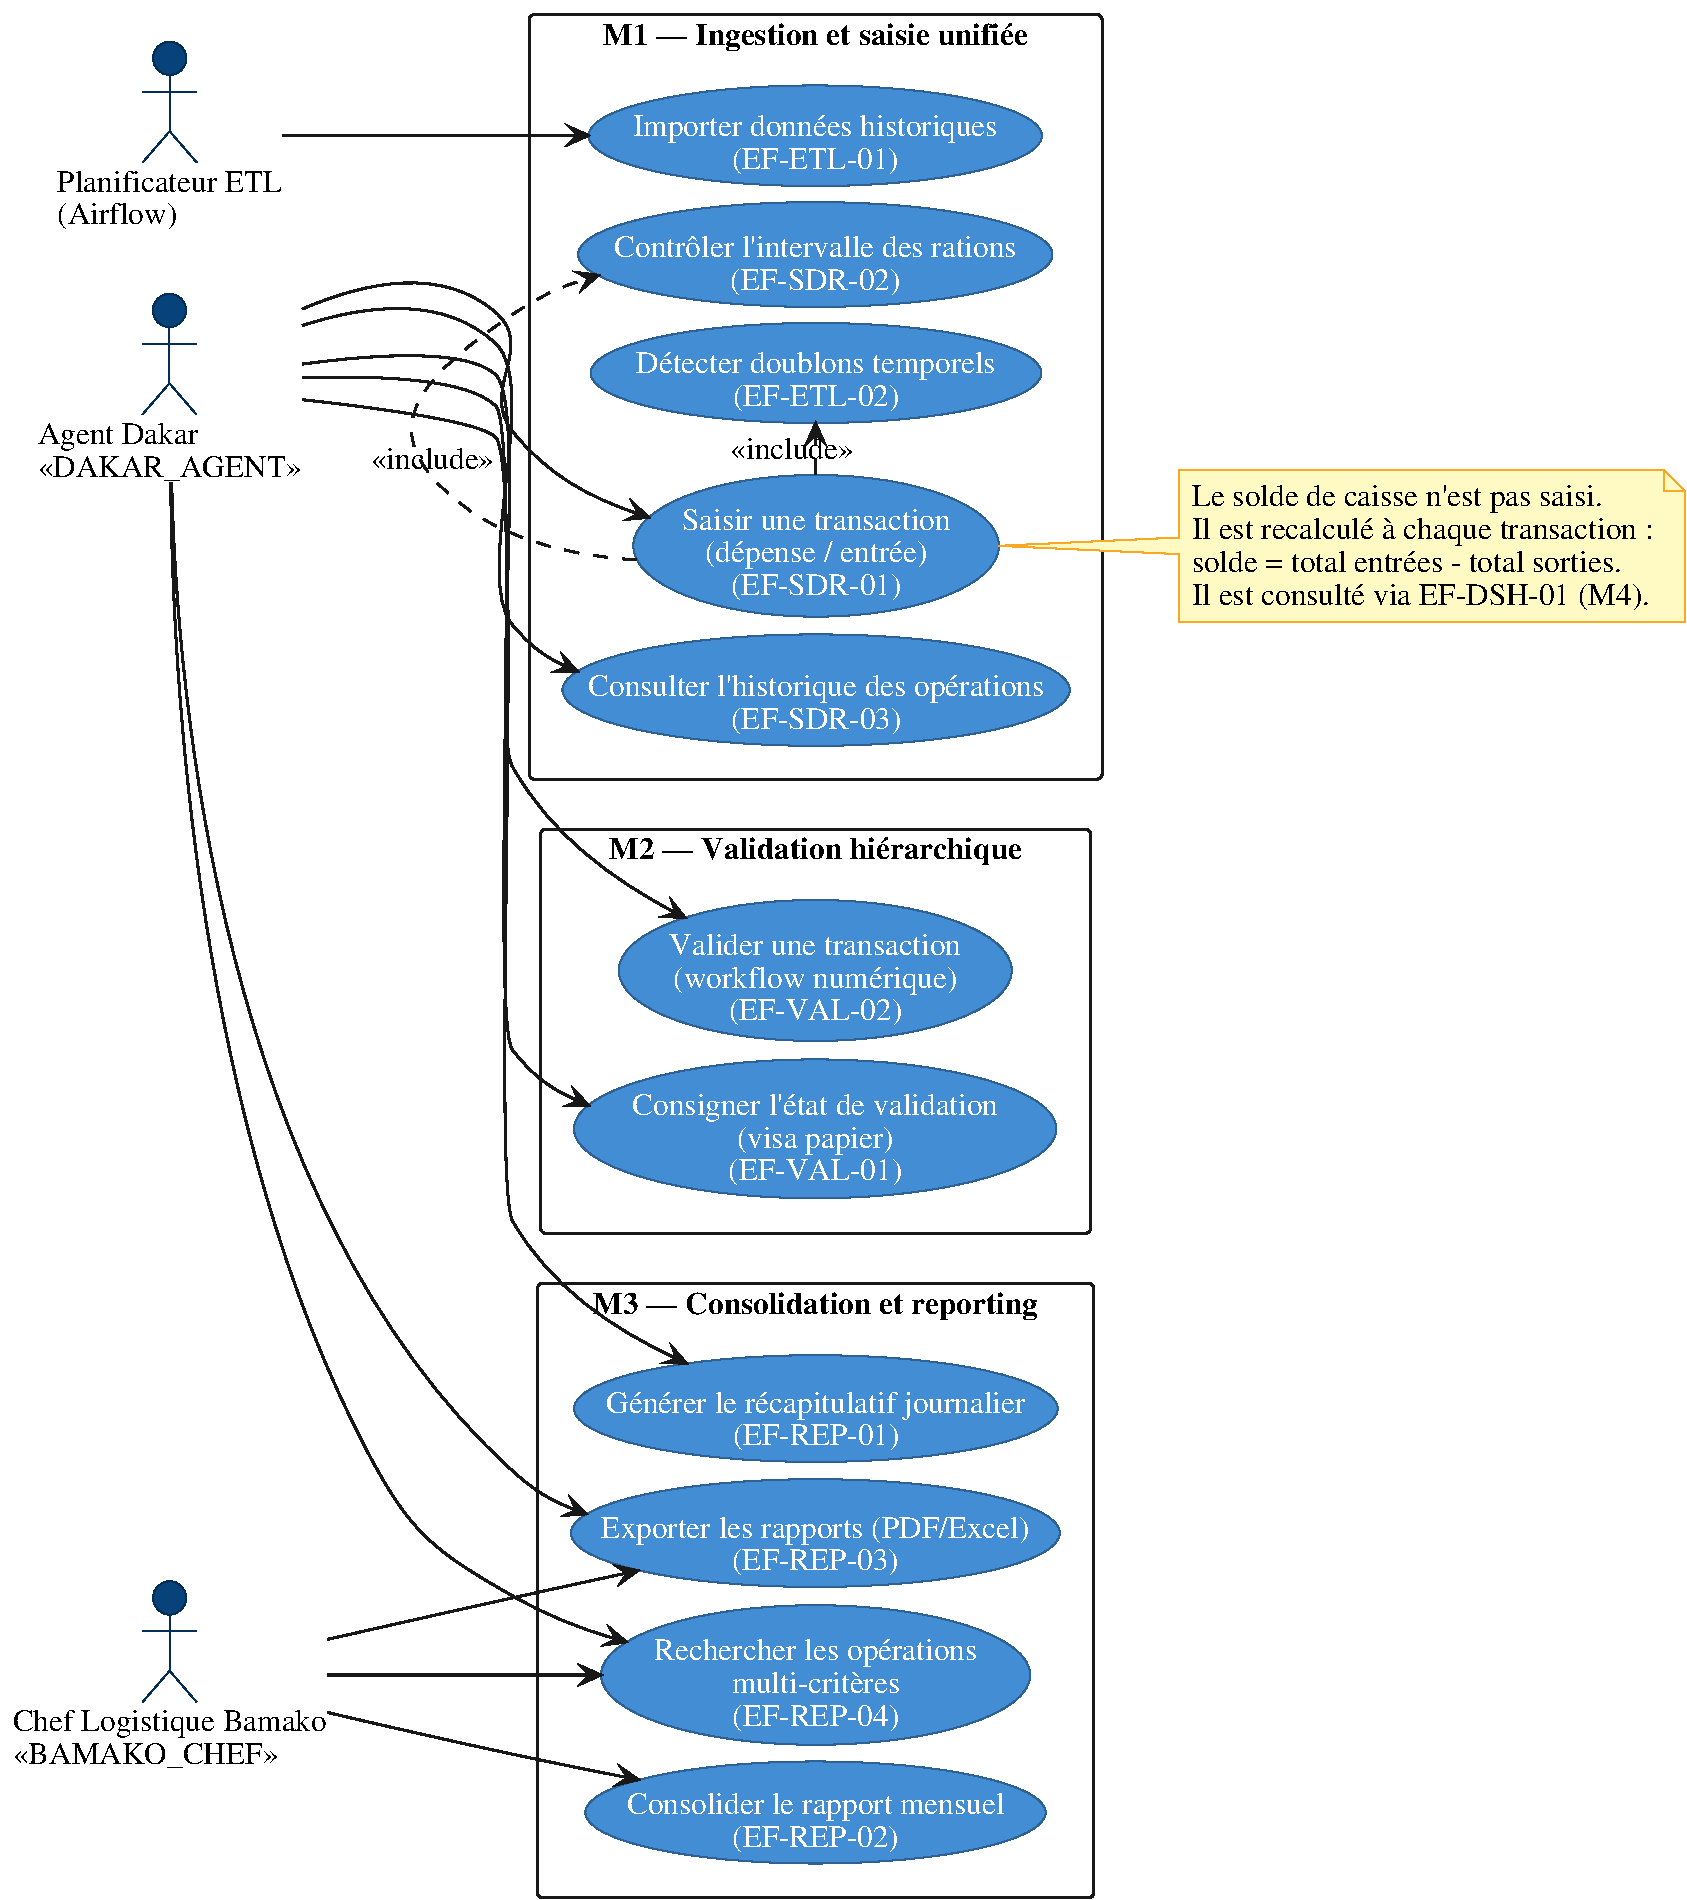
\includegraphics[width=\textwidth,height=0.88\textheight,keepaspectratio]{figures/fig_cas_utilisation_m1_m3.pdf}
    \caption{Diagramme de cas d'utilisation, modules M1 à M3 (Ingestion, Validation, Reporting), plateforme SOYAFF}
    \label{fig:cas_utilisation_1}
    \source{Schéma de l'auteur}
\end{figure}

\begin{figure}[H]
    \centering
    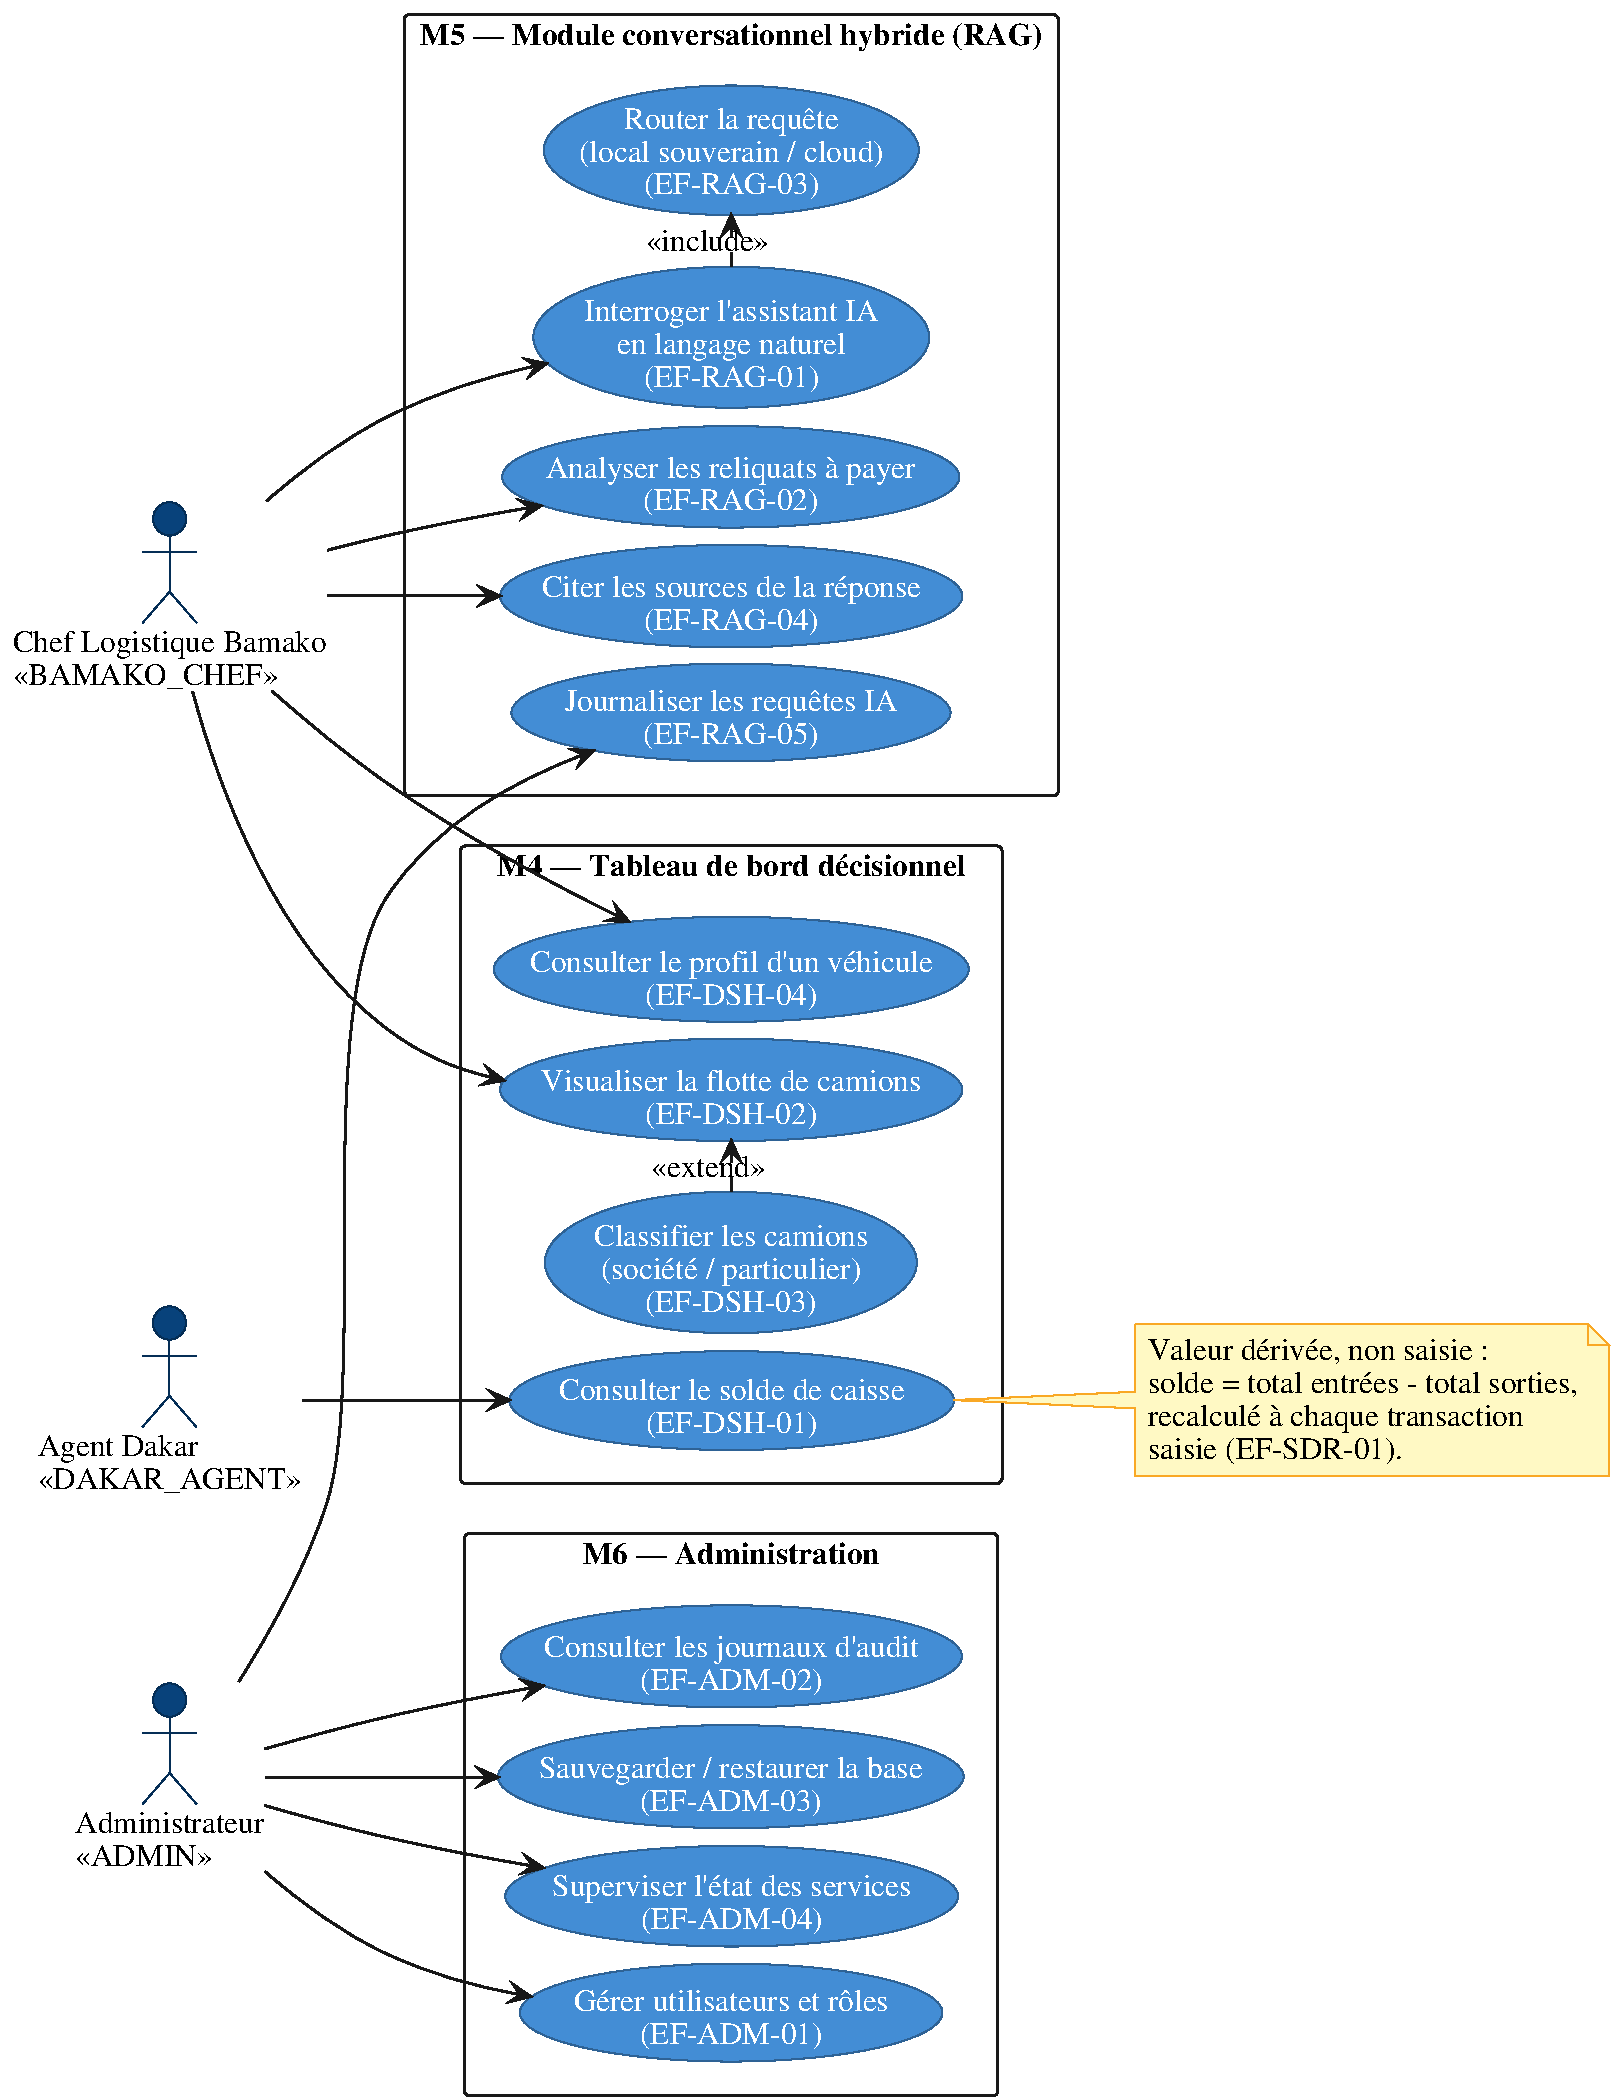
\includegraphics[width=\textwidth,height=0.88\textheight,keepaspectratio]{figures/fig_cas_utilisation_m4_m6.pdf}
    \caption{Diagramme de cas d'utilisation, modules M4 à M6 (Tableau de bord, RAG, Administration), plateforme SOYAFF}
    \label{fig:cas_utilisation_2}
    \source{Schéma de l'auteur}
\end{figure}

\subsection{Modèle de classes du domaine}
\label{sec:classes_domaine}
Le diagramme de classes du domaine métier (Figure~\ref{fig:classes_domaine}) modélise les concepts manipulés par la plateforme, à un niveau d'abstraction conceptuel et non celui du schéma physique de base de données présenté à la section~\ref{chap:architecture}. Les noms de classes et d'attributs sont volontairement alignés sur les tables et colonnes réelles de la base PostgreSQL, afin d'assurer la cohérence entre l'analyse et la réalisation. La classe \texttt{Validation} y figure avec le stéréotype \guillemotleft~conceptuel~\guillemotright~: elle matérialise les exigences \texttt{EF-VAL-01/02} sans préjuger d'une persistance déjà implémentée, cet aspect étant traité au chapitre~\ref{chap:realisation}.

Le modèle s'articule autour de la classe centrale \texttt{Transaction}, qui matérialise tout mouvement financier ou opérationnel. Une \texttt{Transaction} \emph{concerne} un \texttt{Camion} (multiplicité 1 côté camion, chaque camion pouvant porter un nombre indéterminé de transactions), lui-même \emph{conduit} par un \texttt{Chauffeur} : cette chaîne permet de reconstituer le coût réel par véhicule et par chauffeur, indicateur central absent du système actuel (cf. §\ref{sec:recueil}). La classe \texttt{BonLivraison} agrège les transactions relatives à un même chargement et est reliée aux \texttt{Produit} transportés par une association plusieurs-à-plusieurs, un bon regroupant plusieurs références et une référence figurant sur plusieurs bons. Cette association porte une donnée qui n'appartient ni au bon ni au produit, la quantité livrée : elle est donc modélisée par la classe d'association \texttt{BonLivraisonProduit}, rattachée au lien entre les deux classes. L'attribut \texttt{/solde\_progressif} de \texttt{Transaction} est noté comme attribut dérivé : il n'est jamais saisi, mais calculé à partir des entrées et des sorties. Enfin, la classe \texttt{Validation}, ici purement conceptuelle, s'attache à la \texttt{Transaction} qu'elle qualifie sans en présumer la persistance physique. Les classes \texttt{Utilisateur}, \texttt{RequeteIA} et \texttt{AuditLog} constituent le socle transverse de sécurité et de traçabilité (RBAC, journalisation IA et piste d'audit) exigé par les \texttt{ENF-SEC} et \texttt{EF-RAG-05}. L'ensemble \texttt{CategorieOperation} est modélisé comme une énumération (et non une entité), reflétant son statut de colonne typée dans le schéma relationnel.

\begin{landscape}
\begin{figure}[p]
    \centering
    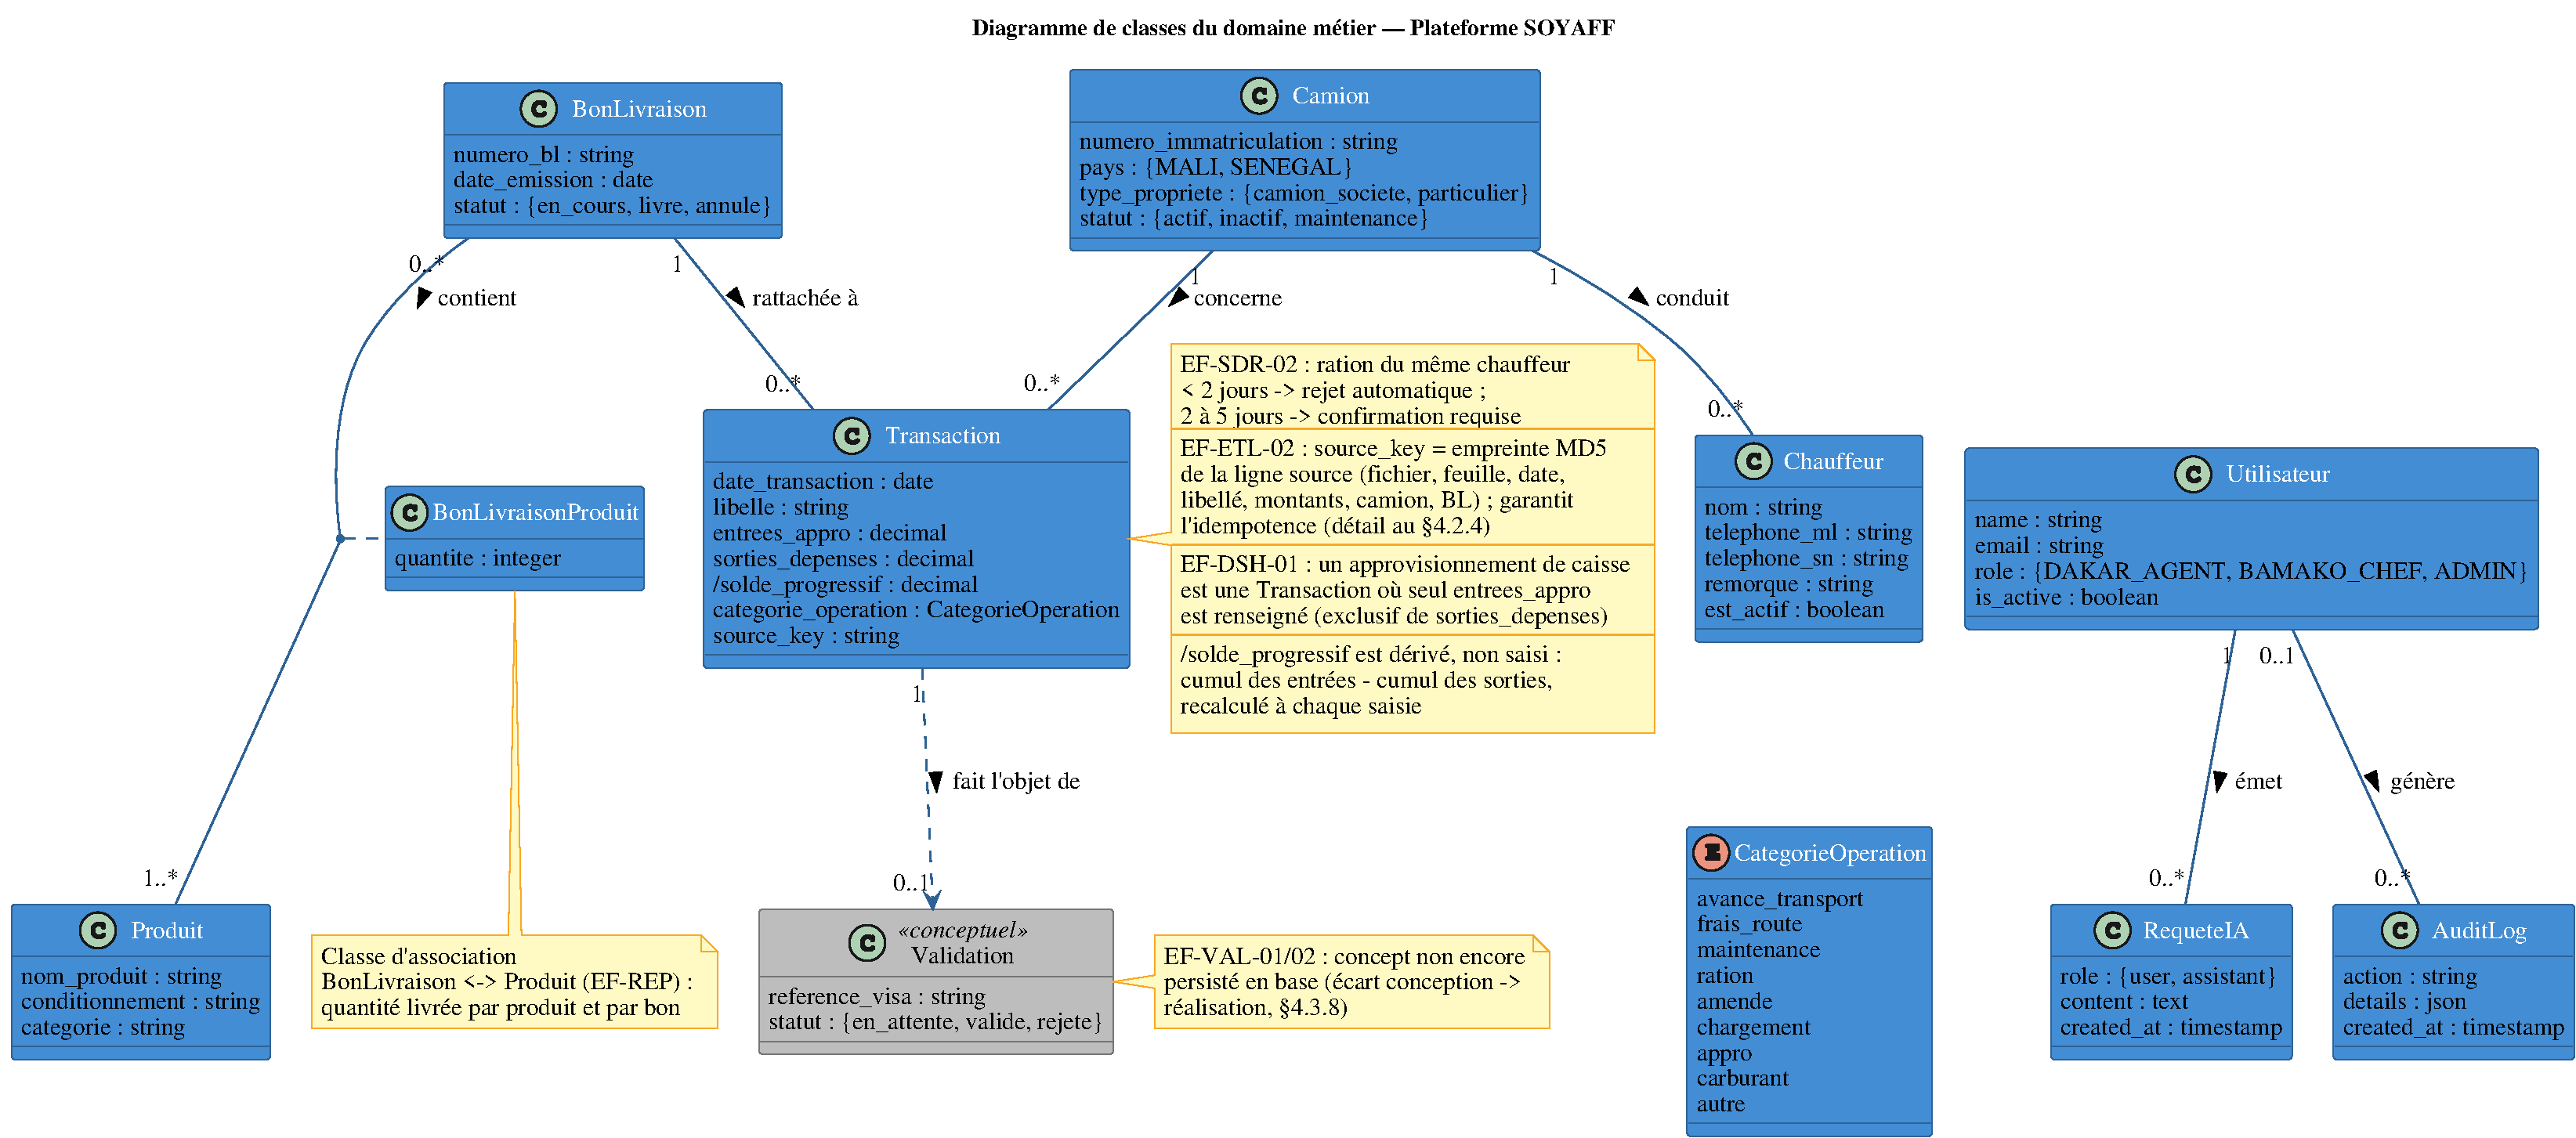
\includegraphics[width=\linewidth,height=0.86\textheight,keepaspectratio]{figures/fig_classes_domaine.pdf}
    \caption{Diagramme de classes du domaine métier, plateforme SOYAFF}
    \label{fig:classes_domaine}
    \source{Schéma de l'auteur}
\end{figure}
\end{landscape}

\subsection{Comportements dynamiques}
\label{sec:sequences}
Les deux scénarios suivants ont été retenus pour leur caractère structurant : le premier opérationnalise les garde-fous métier de la saisie (§\ref{sec:recueil}), le second matérialise la définition d'architecture \guillemotleft~hybride~\guillemotright~qui porte l'hypothèse H2.

\subsubsection{Séquence de saisie d'une dépense avec contrôles}
\label{subsec:seq_saisie}
La Figure~\ref{fig:seq_saisie} détaille le scénario de saisie d'une dépense, avec ses deux garde-fous : la détection de doublons temporels (\texttt{EF-ETL-02}) et le contrôle de l'intervalle entre deux rations (\texttt{EF-SDR-02}), modélisés par des fragments combinés \texttt{alt}.

\begin{figure}[H]
    \centering
    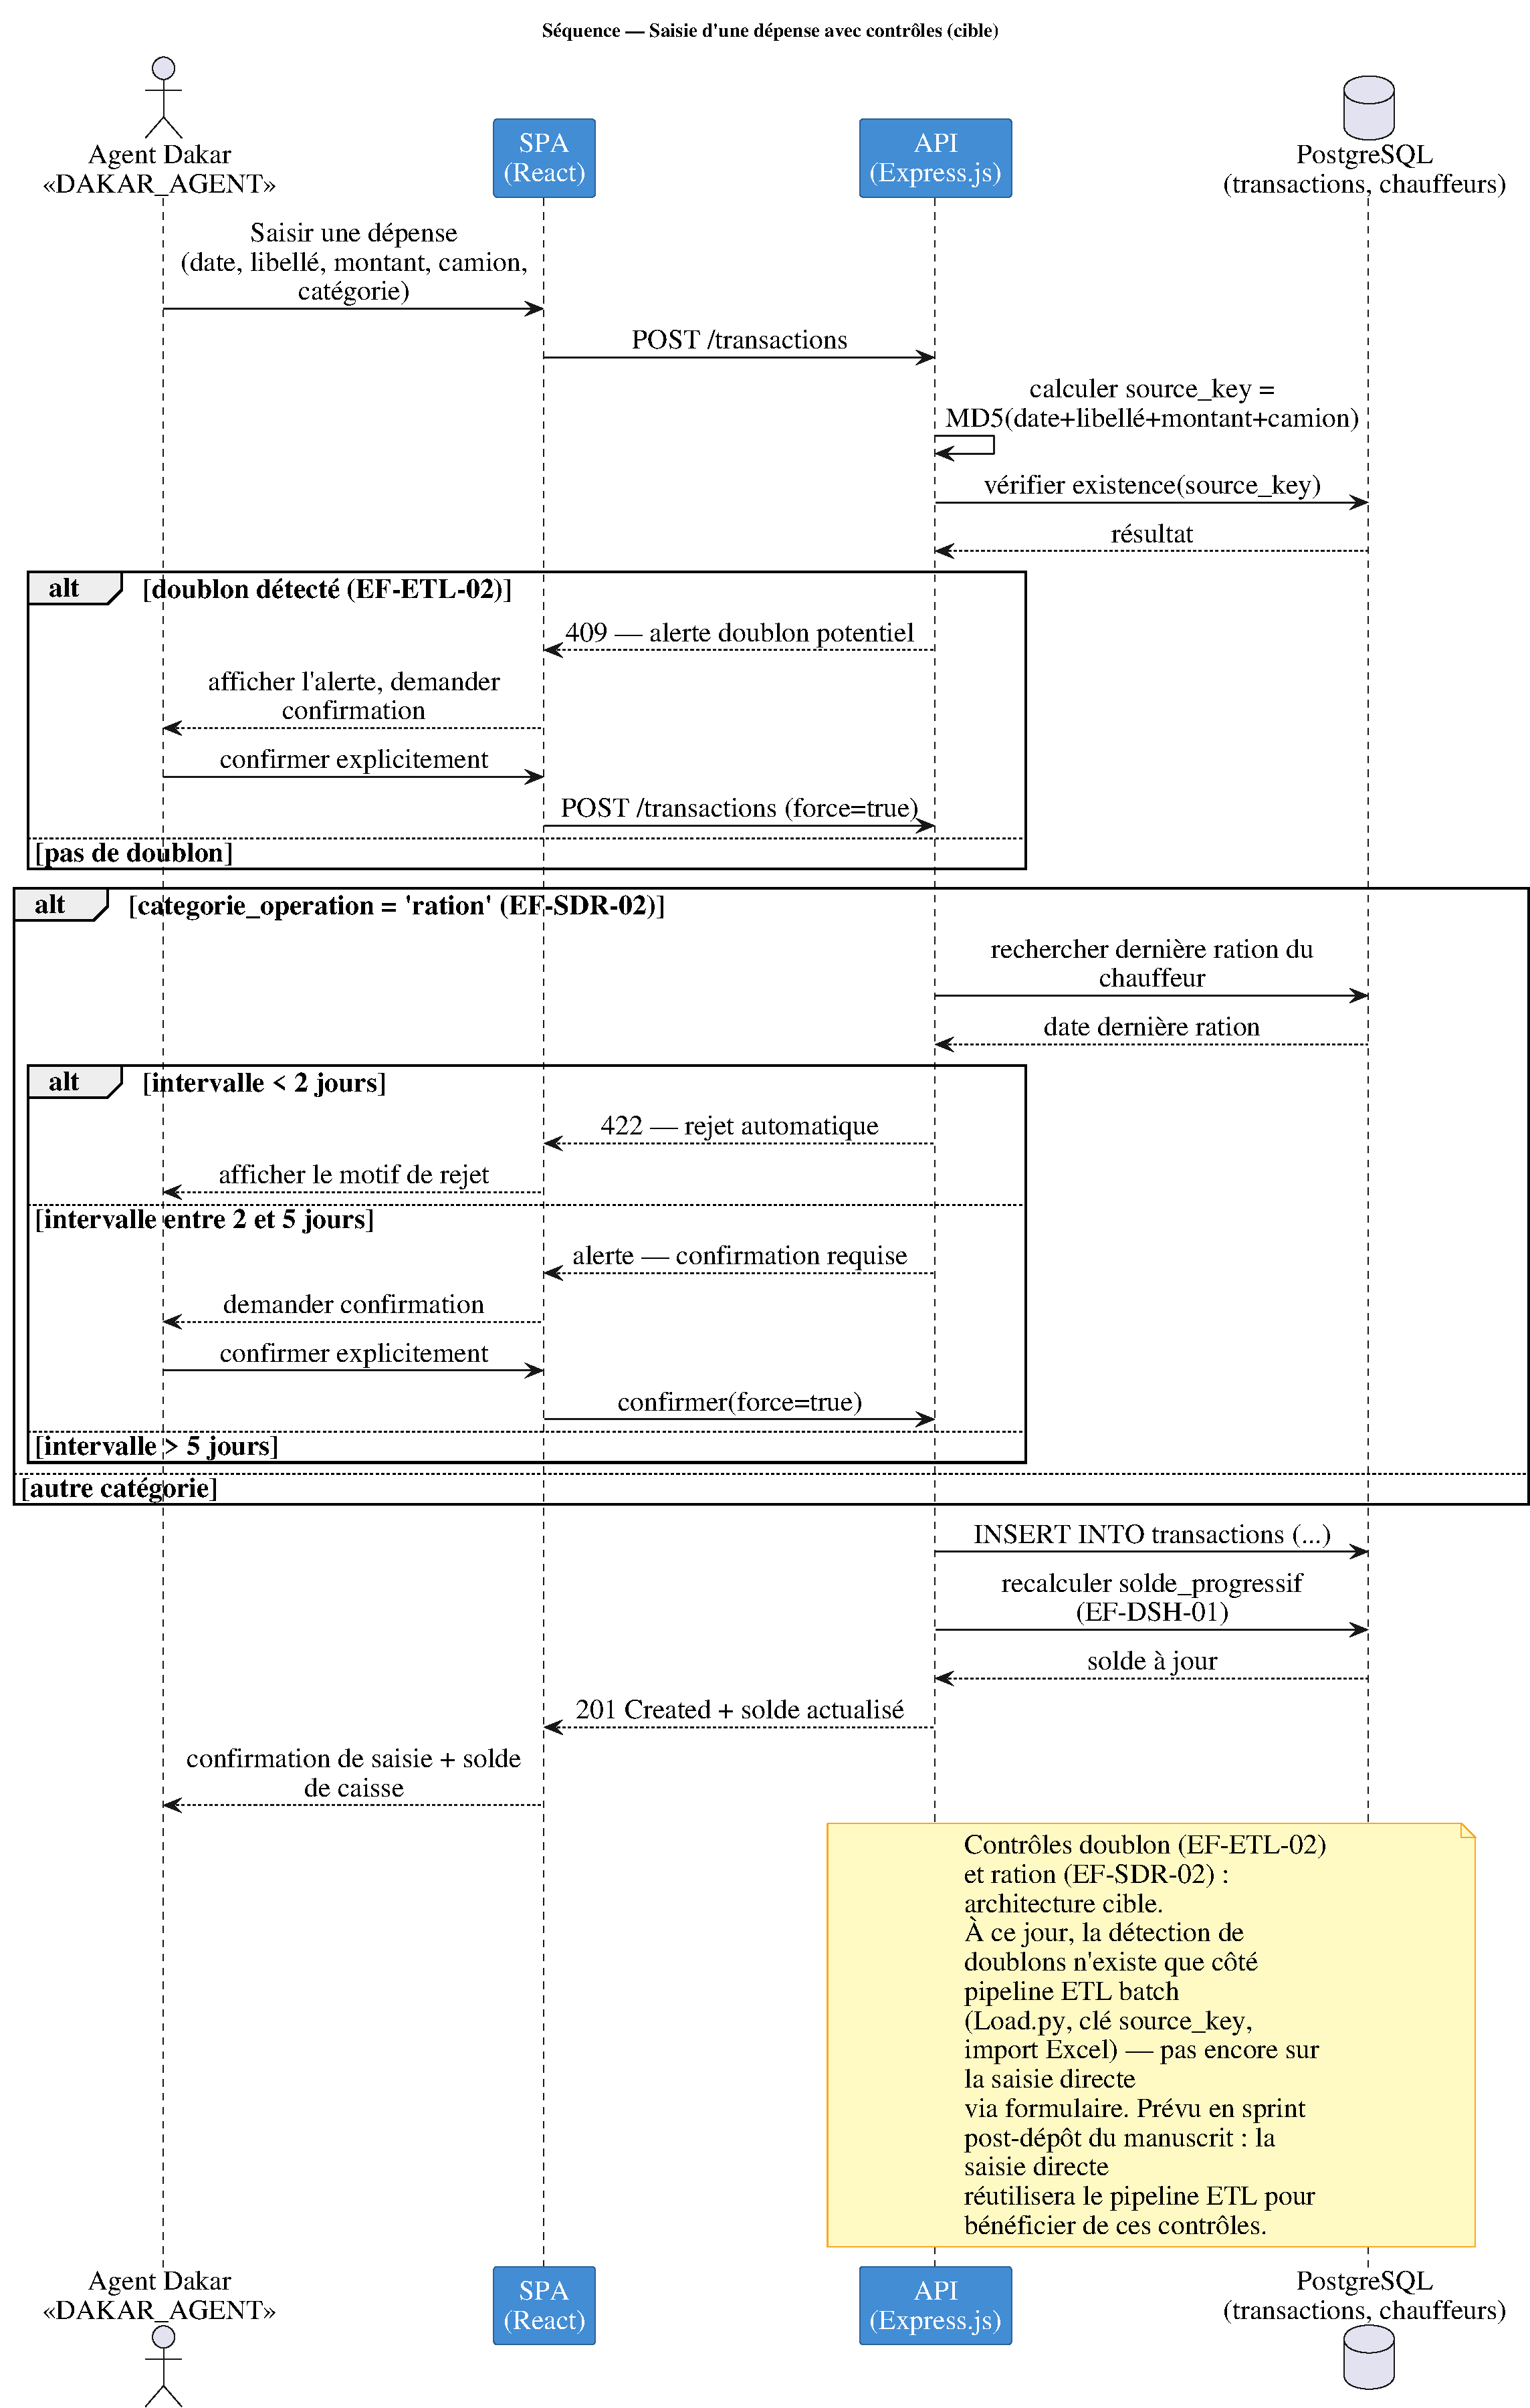
\includegraphics[width=\textwidth,height=0.88\textheight,keepaspectratio]{figures/fig_seq_saisie_controles.pdf}
    \caption{Séquence : saisie d'une dépense avec contrôles}
    \label{fig:seq_saisie}
    \source{Schéma de l'auteur}
\end{figure}

\subsubsection{Séquence de requête RAG avec routage hybride}
\label{subsec:seq_rag}
La Figure~\ref{fig:seq_rag} illustre le traitement d'une requête en langage naturel adressée à l'agent conversationnel, depuis sa soumission jusqu'à la restitution de la réponse. Le routage entre chemin local souverain et chemin cloud (\texttt{EF-RAG-03}) y est représenté par un fragment \texttt{alt} conditionné par l'analyse de sensibilité réalisée par l'orchestrateur n8n.

\begin{landscape}
\begin{figure}[p]
    \centering
    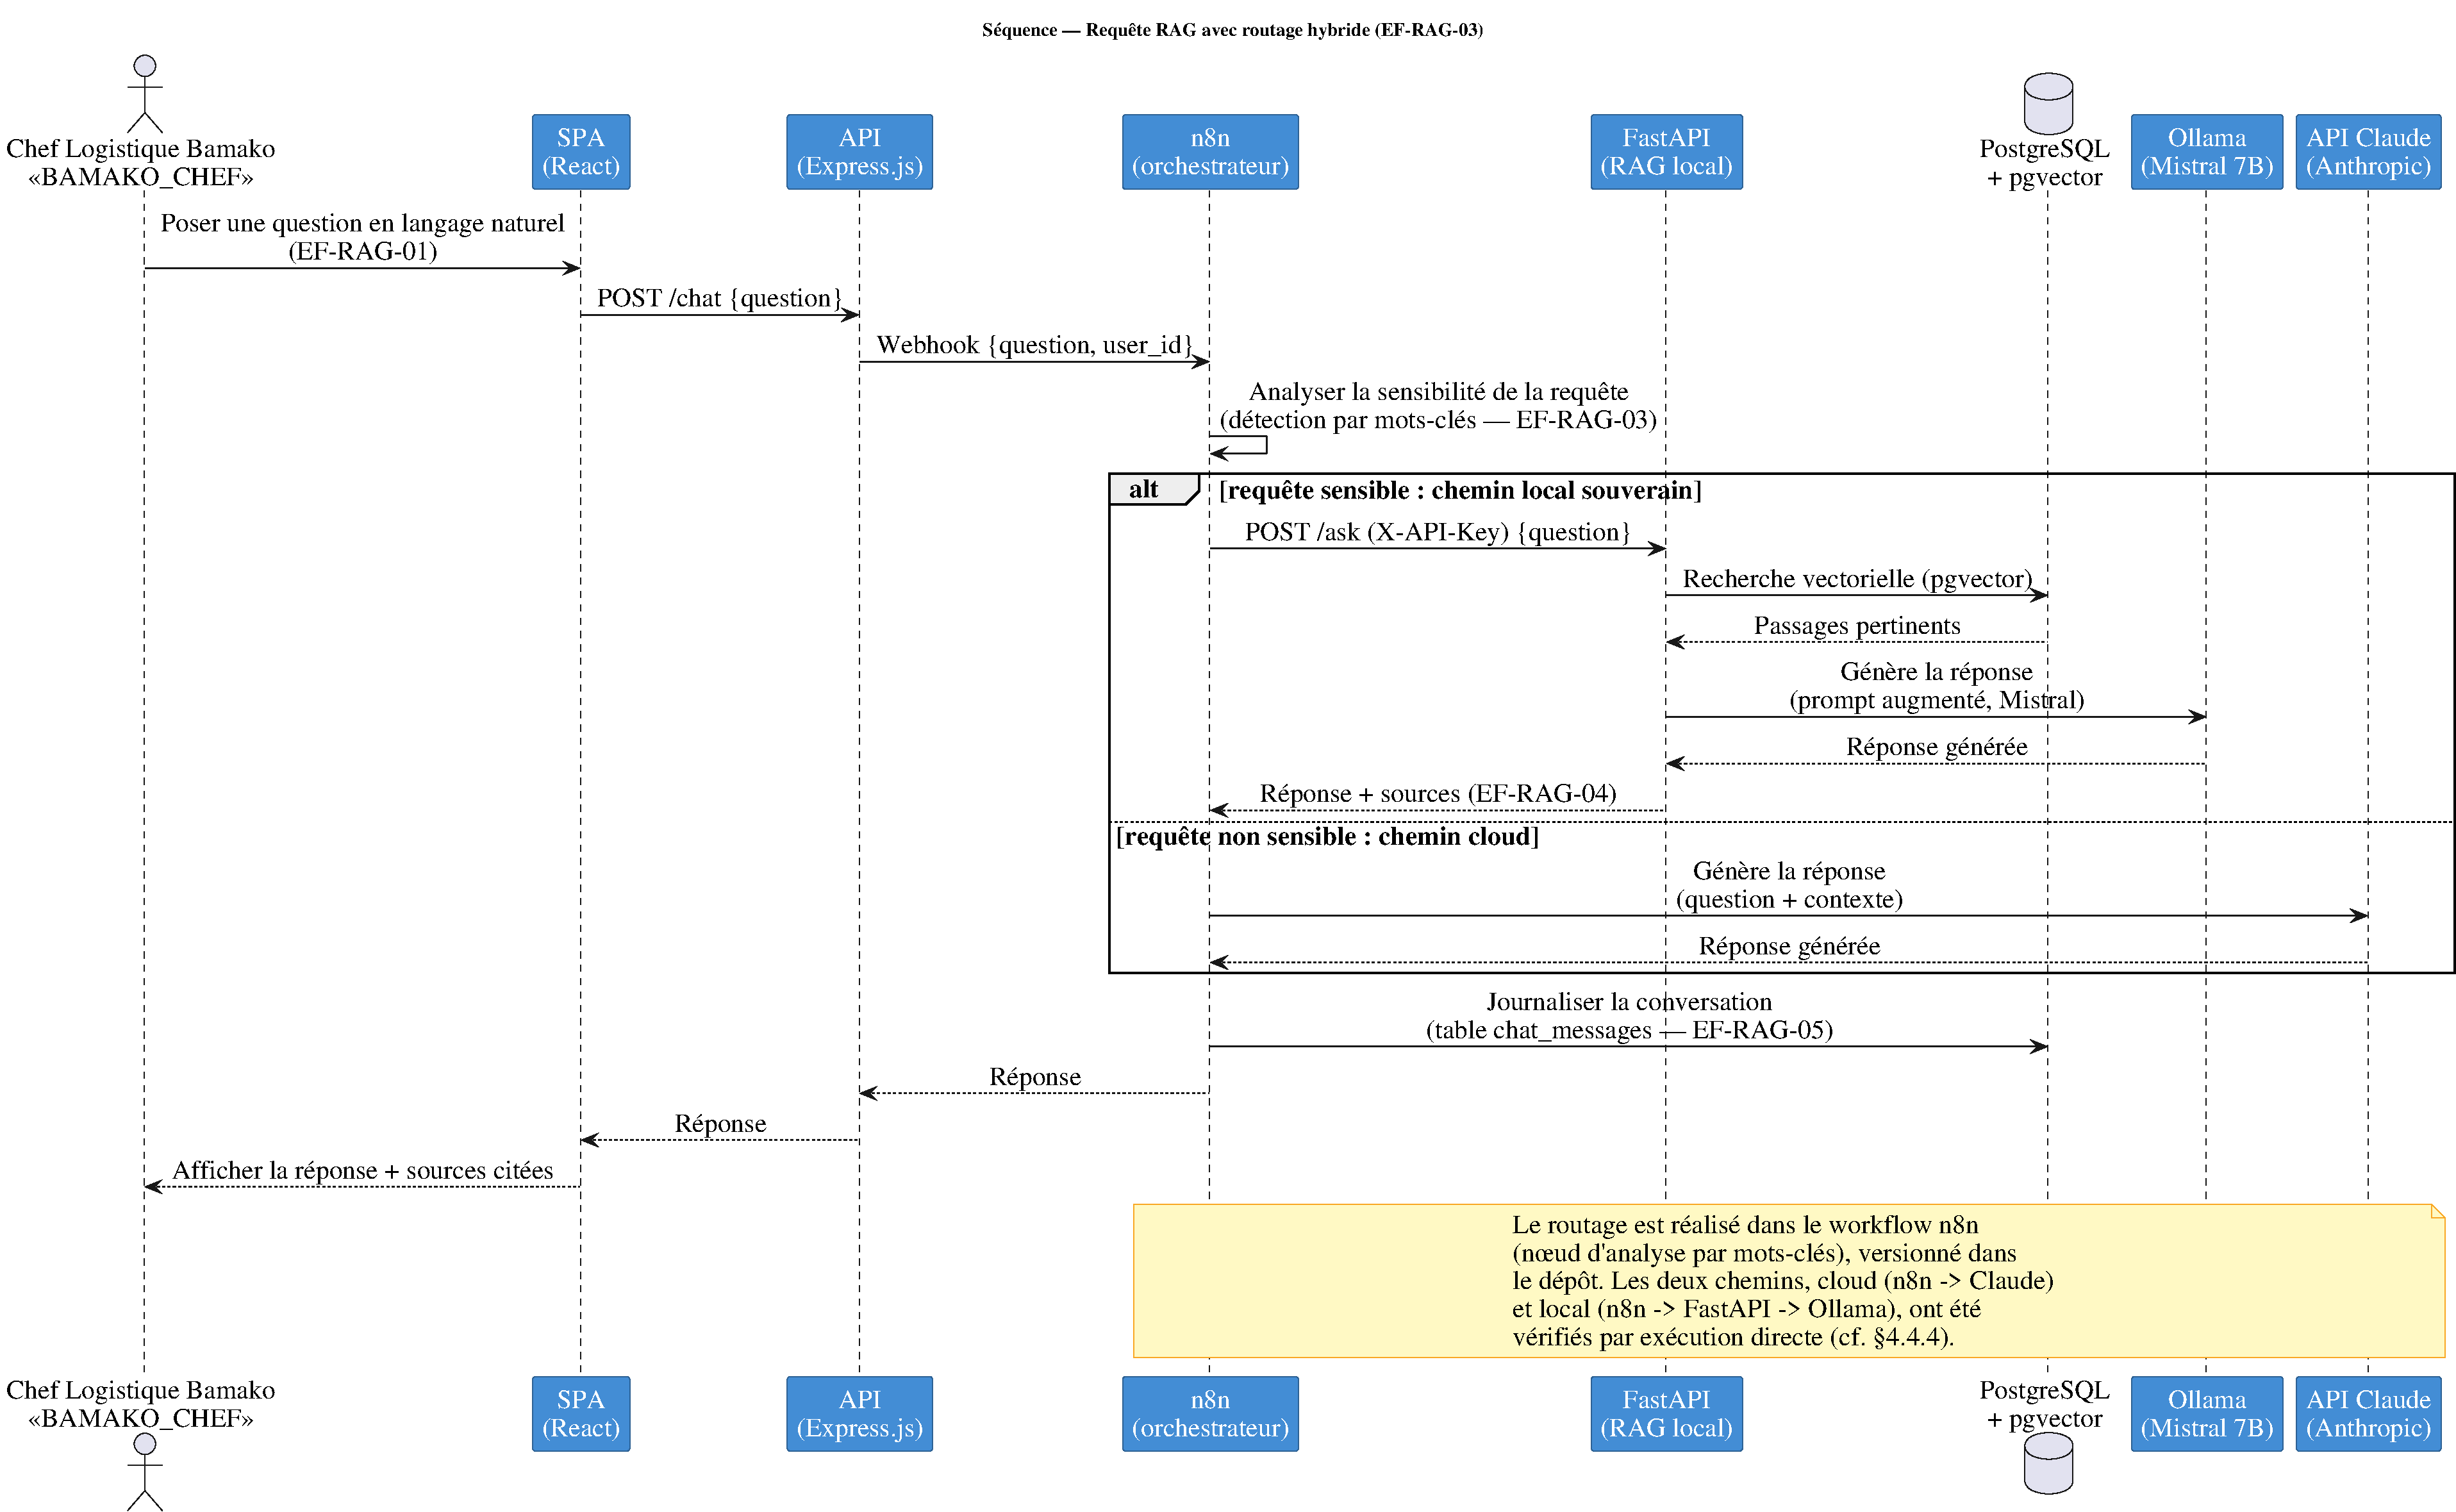
\includegraphics[width=\linewidth,height=0.86\textheight,keepaspectratio]{figures/fig_seq_rag_hybride.pdf}
    \caption{Séquence : requête RAG avec routage hybride}
    \label{fig:seq_rag}
    \source{Schéma de l'auteur}
\end{figure}
\end{landscape}

\subsection{Workflow de validation}
\label{sec:activite_validation}
Les deux séquences précédentes décrivent des interactions synchrones, centrées sur une requête unique. Le processus de validation, lui, est un flux de travail asynchrone avec plusieurs acteurs et des points de décision : le diagramme d'activité est le formalisme adapté.

Les Figures~\ref{fig:activite_validation_actuelle} et~\ref{fig:activite_validation_cible} présentent, sous forme de diagrammes d'activité à couloirs, le circuit de validation observé sur le terrain et le circuit dématérialisé cible. Le premier correspond à l'exigence \textit{Must} \texttt{EF-VAL-01} ; le second, à l'exigence \textit{Should} \texttt{EF-VAL-02}, dont la priorisation reflète le maintien du circuit papier comme référence juridiquement opposable durant la phase de transition (§\ref{sec:synthese_tracabilite}).

\begin{figure}[H]
    \centering
    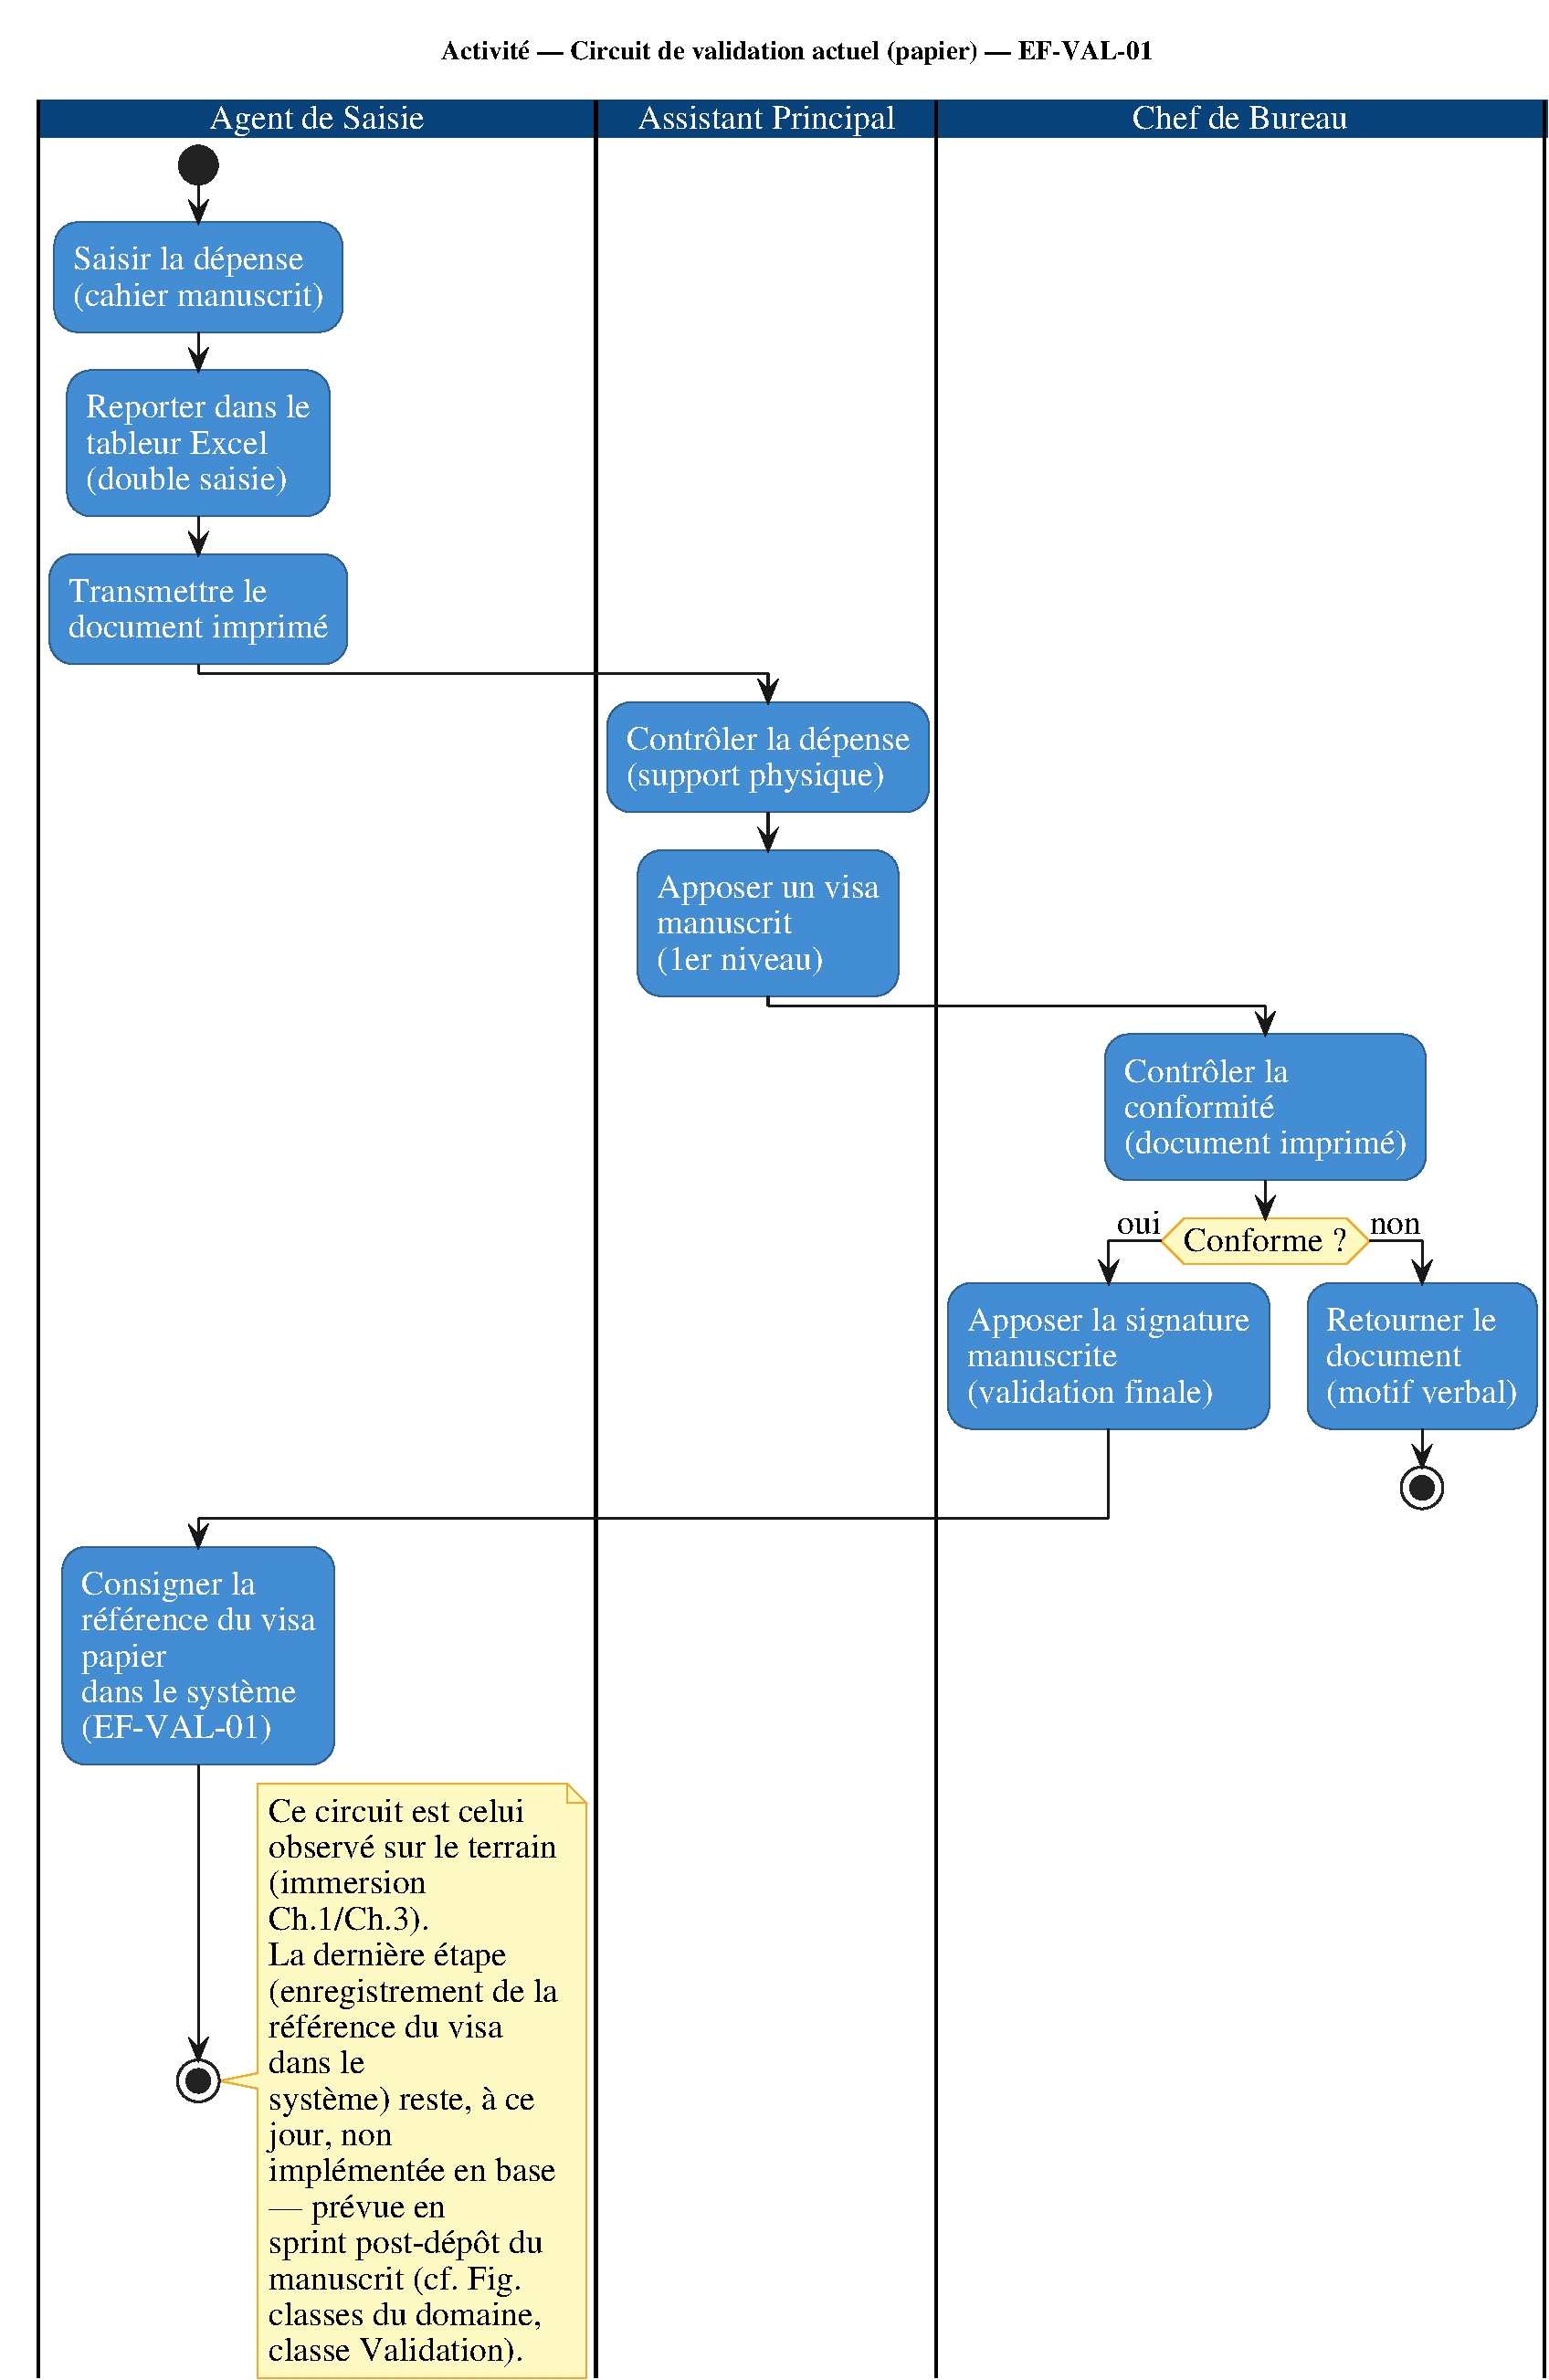
\includegraphics[width=\textwidth,height=0.88\textheight,keepaspectratio]{figures/fig_activite_validation_actuelle.pdf}
    \caption{Activité : circuit de validation actuel (papier)}
    \label{fig:activite_validation_actuelle}
    \source{Schéma de l'auteur}
\end{figure}

\begin{figure}[H]
    \centering
    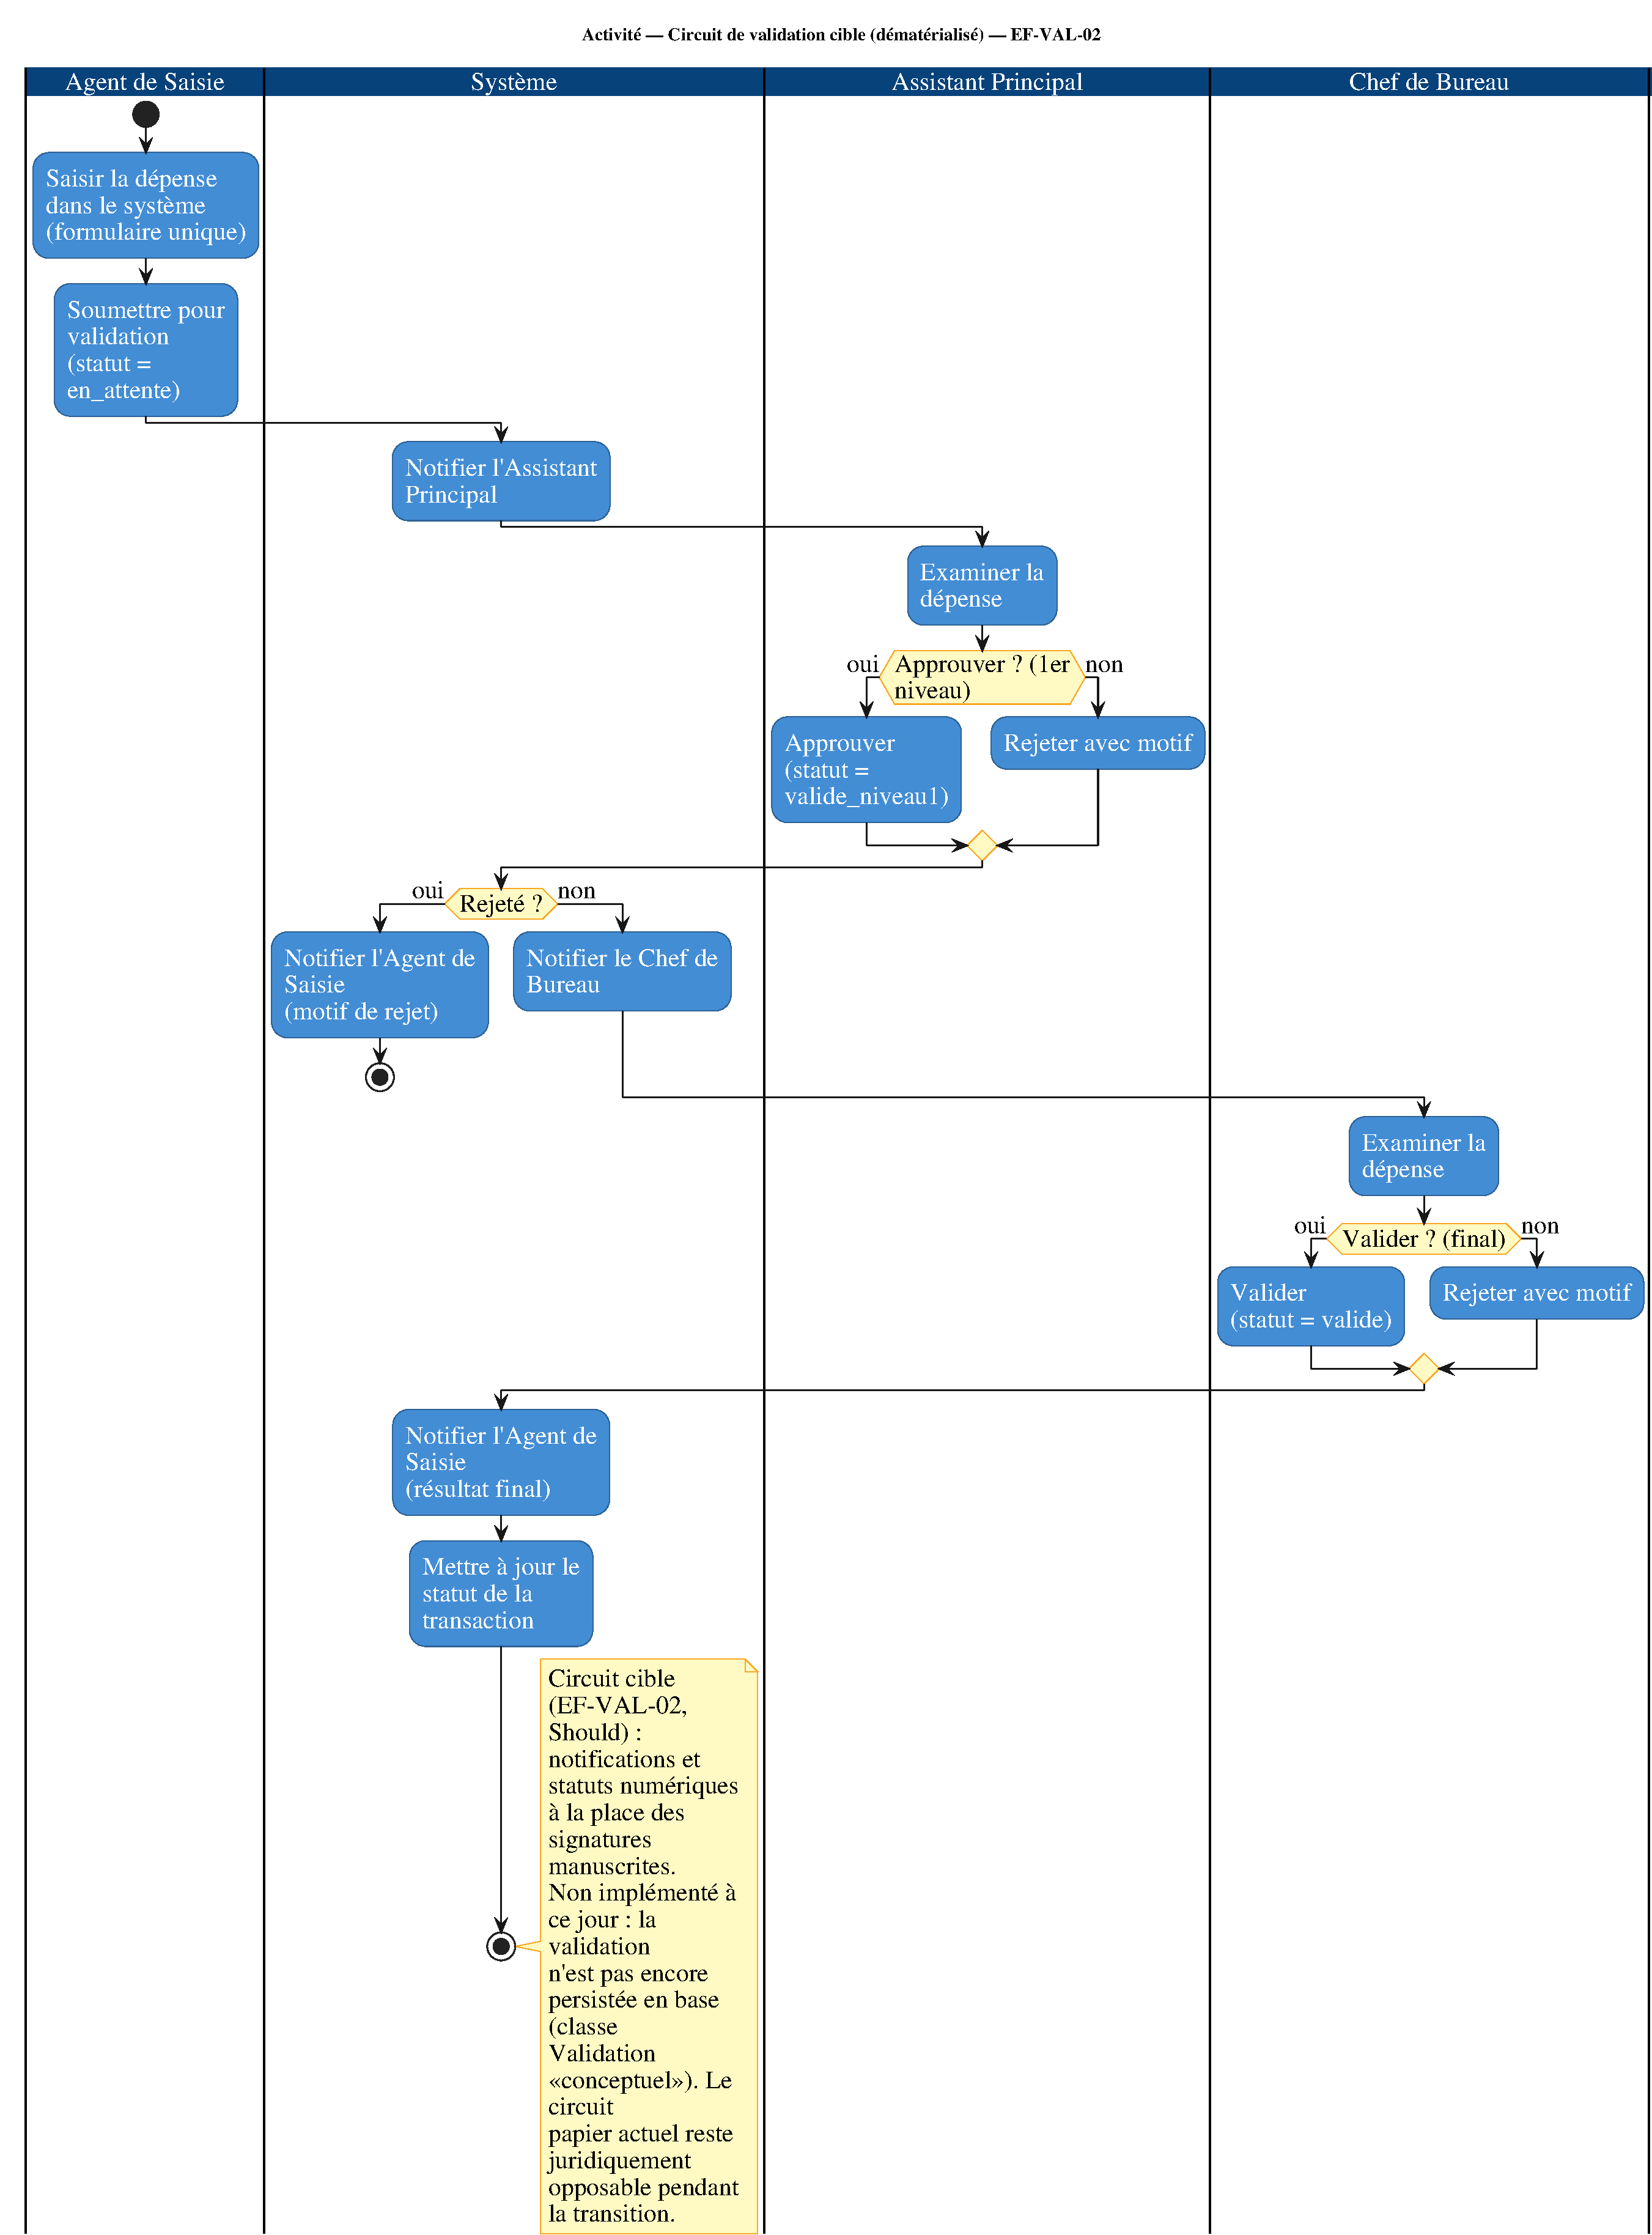
\includegraphics[width=\textwidth,height=0.88\textheight,keepaspectratio]{figures/fig_activite_validation_cible.pdf}
    \caption{Activité : circuit de validation cible (dématérialisé)}
    \label{fig:activite_validation_cible}
    \source{Schéma de l'auteur}
\end{figure}


\section{Architecture de la solution (C4 et ADR)}
\label{chap:architecture}

Cette section présente l'architecture logicielle et d'infrastructure retenue pour la plateforme SOYAFF, selon les trois premiers niveaux du modèle C4 (contexte, conteneurs, composants), complétés par une vue de déploiement de l'infrastructure de production.

\subsection{Vue de contexte}
\label{sec:c4_contexte}
La Figure~\ref{fig:c4_contexte} situe la plateforme SOYAFF parmi les systèmes avec lesquels elle interagit : les trois rôles utilisateurs, l'API Claude d'Anthropic pour le traitement cloud des requêtes non sensibles (\texttt{EF-RAG-03}), les fichiers Excel legacy servant de source à l'import historique (\texttt{EF-ETL-01}), et l'application \texttt{kiri.app} déjà en usage, dont le périmètre disjoint est explicitement représenté (§\ref{sec:recueil}).

\begin{figure}[H]
    \centering
    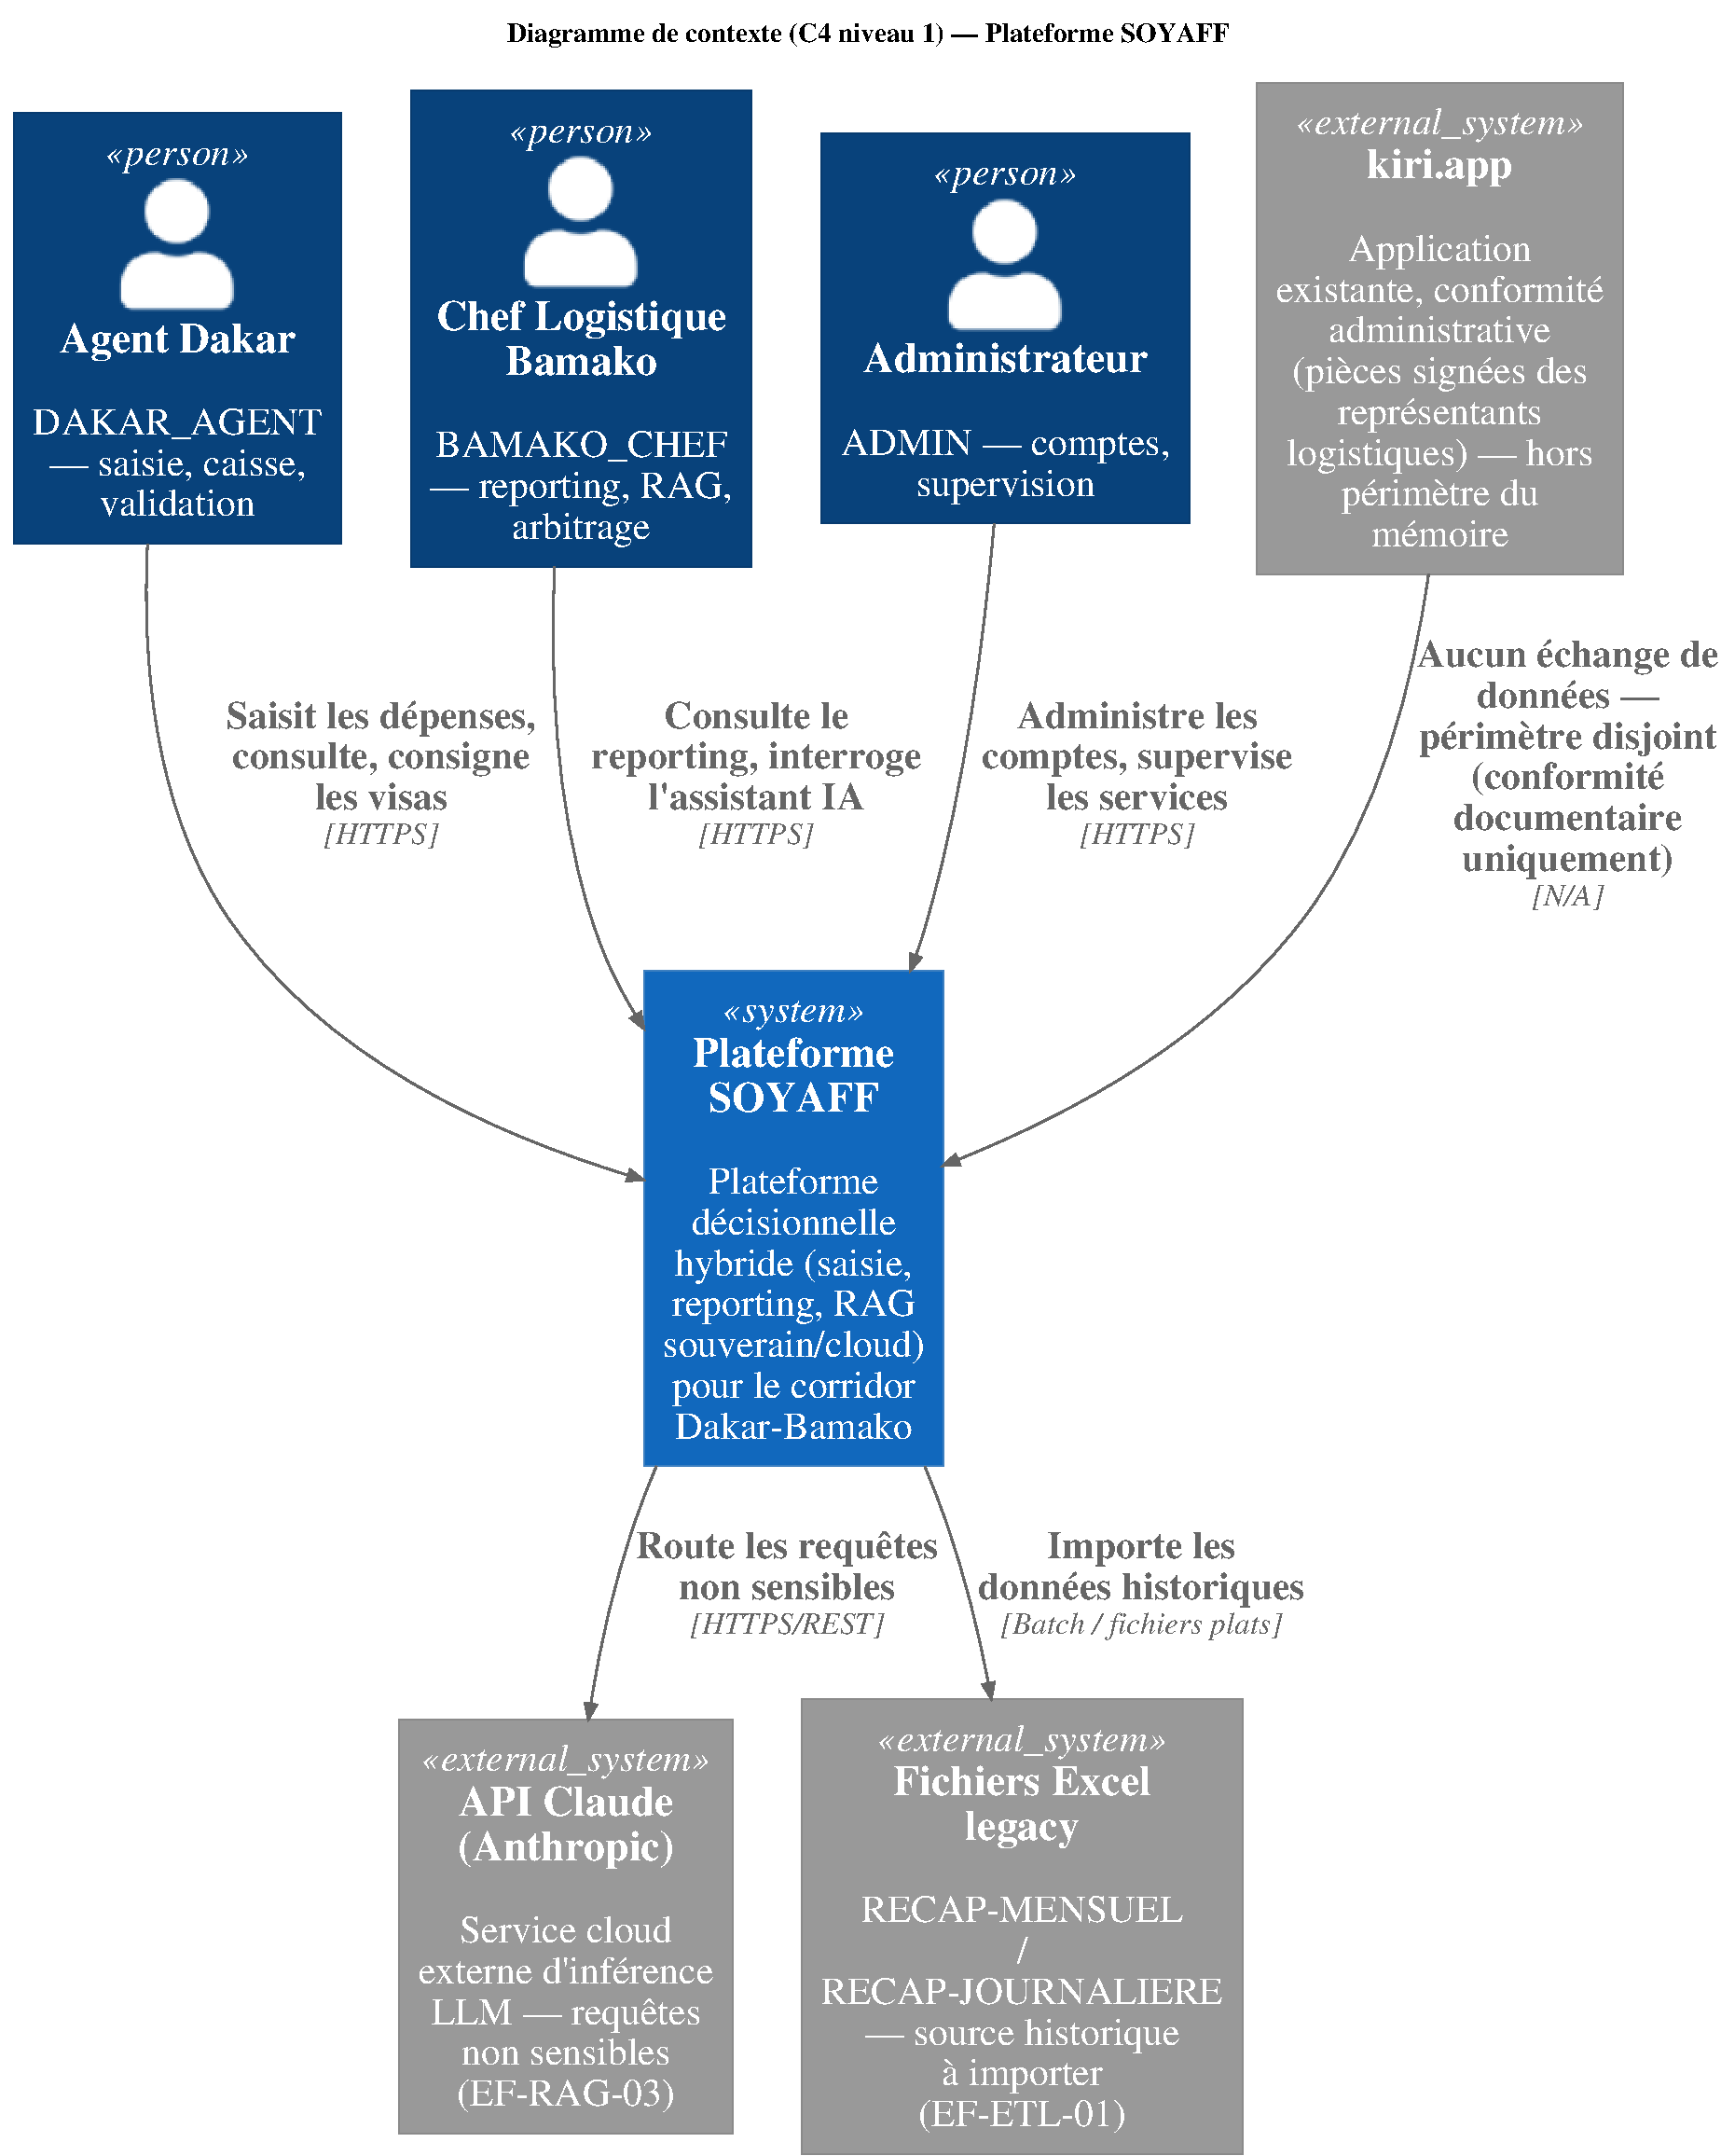
\includegraphics[width=\textwidth,height=0.88\textheight,keepaspectratio]{figures/fig_c4_contexte.pdf}
    \caption{Diagramme de contexte (C4 niveau 1), plateforme SOYAFF}
    \label{fig:c4_contexte}
    \source{Schéma de l'auteur}
\end{figure}

\subsection{Vue de conteneurs}
\label{sec:c4_conteneurs}
La Figure~\ref{fig:c4_conteneurs} détaille les conteneurs applicatifs déployés au sein du périmètre souverain de la plateforme. Le point d'entrée unique du module conversationnel est l'orchestrateur n8n, qui analyse la sensibilité de chaque requête et la route vers le service RAG local (FastAPI, Ollama/Mistral) ou vers l'API Claude cloud, conformément à \texttt{EF-RAG-03}. La conversation est journalisée en base (\texttt{EF-RAG-05}) indépendamment du chemin emprunté.

La frontière «\,périmètre souverain\,» tracée sur la figure n'est pas cosmétique : elle délimite l'ensemble des conteneurs au sein desquels les données métier ne quittent jamais l'infrastructure maîtrisée. Seul le chemin cloud (API Claude) la franchit, et uniquement pour des requêtes préalablement classées non sensibles par l'orchestrateur. Cette étanchéité conditionne la validité des exigences \texttt{ENF-SOUV-01} et \texttt{ENF-SOUV-02}.

\begin{figure}[H]
    \centering
    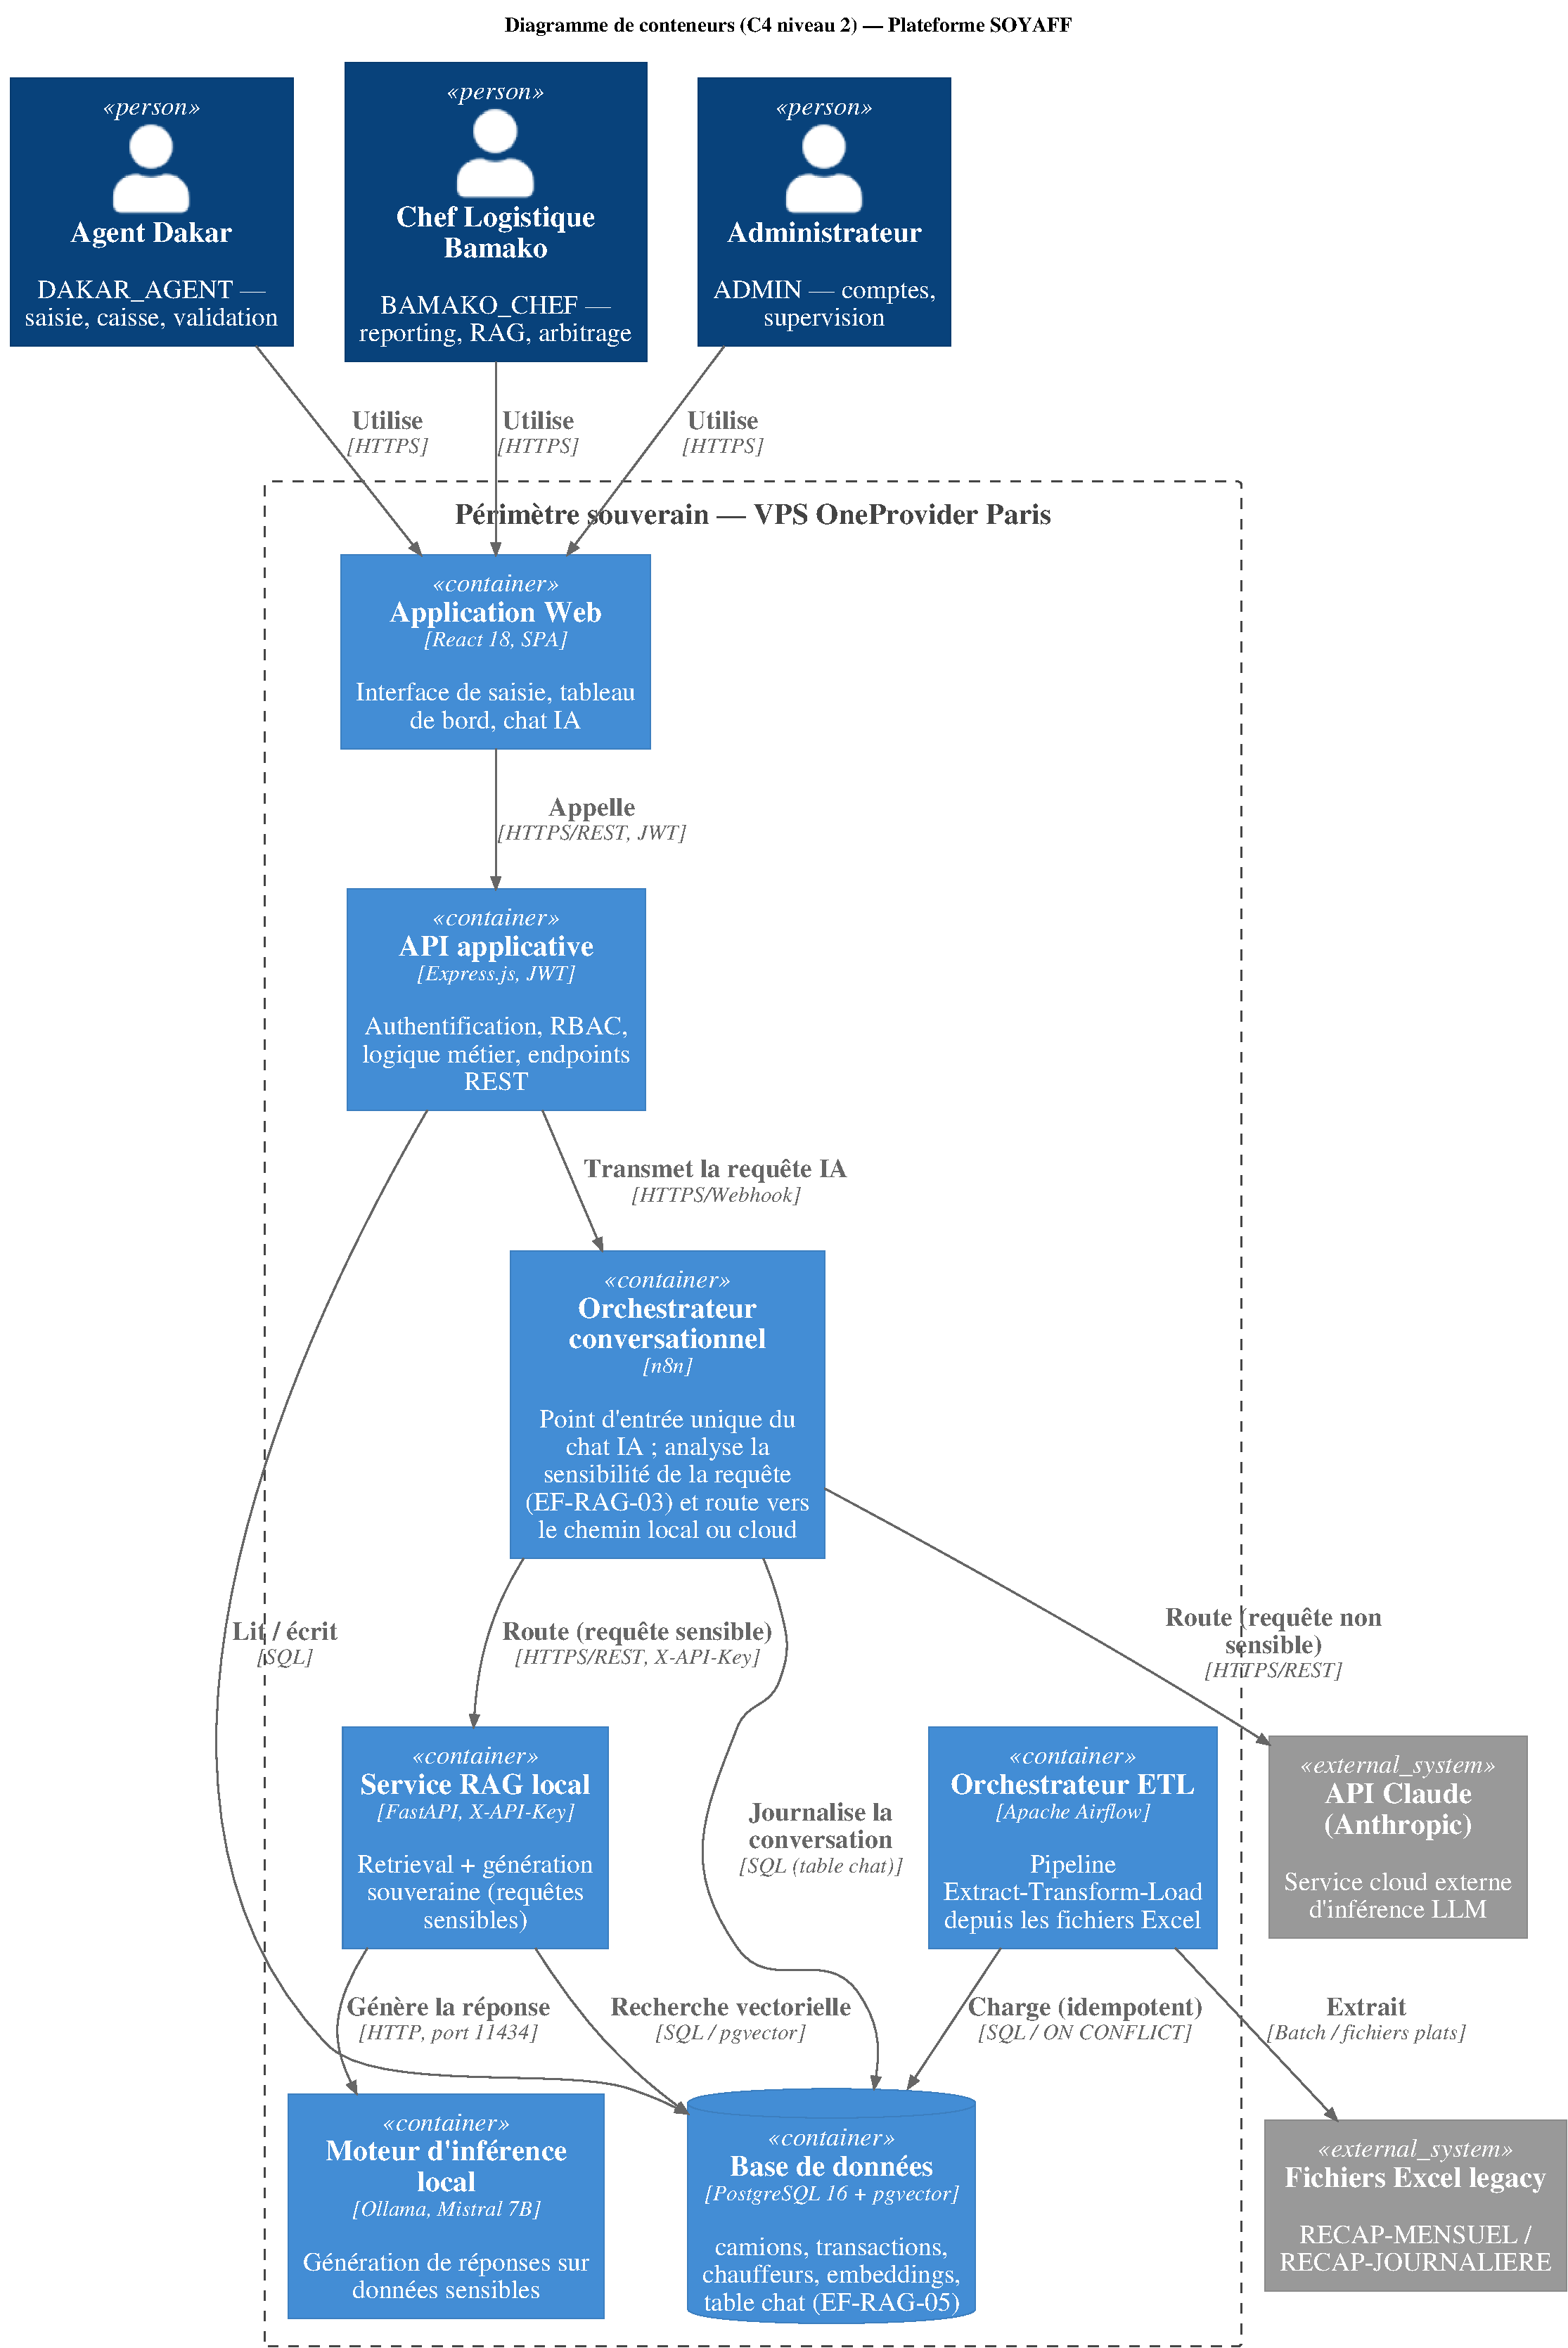
\includegraphics[width=\textwidth,height=0.88\textheight,keepaspectratio]{figures/fig_c4_conteneurs.pdf}
    \caption{Diagramme de conteneurs (C4 niveau 2), plateforme SOYAFF}
    \label{fig:c4_conteneurs}
    \source{Schéma de l'auteur}
\end{figure}

\subsection{Vue de composants : service RAG local}
\label{sec:c4_composants}
Nous ne détaillons le niveau 3 (composants) que pour le conteneur le plus significatif. La Figure~\ref{fig:c4_composants_rag} isole donc les composants internes du service RAG local (FastAPI) : le gestionnaire de requêtes, un composant de réponses SQL directes (comptages, solde), le module de retrieval (filtres SQL puis repli vectoriel \texttt{all-MiniLM-L6-v2}), le constructeur de contexte et le client d'inférence. Les questions de comptage, de solde et de total sont servies sans modèle de langage ; les autres sont confiées à Mistral~7B. Cette vue met aussi en évidence deux écarts à l'exigence de maintenabilité (\texttt{ENF-MAINT-01}, \texttt{ENF-MAINT-02}), détaillés au §\ref{sec:ia_dettes}.

\begin{figure}[H]
    \centering
    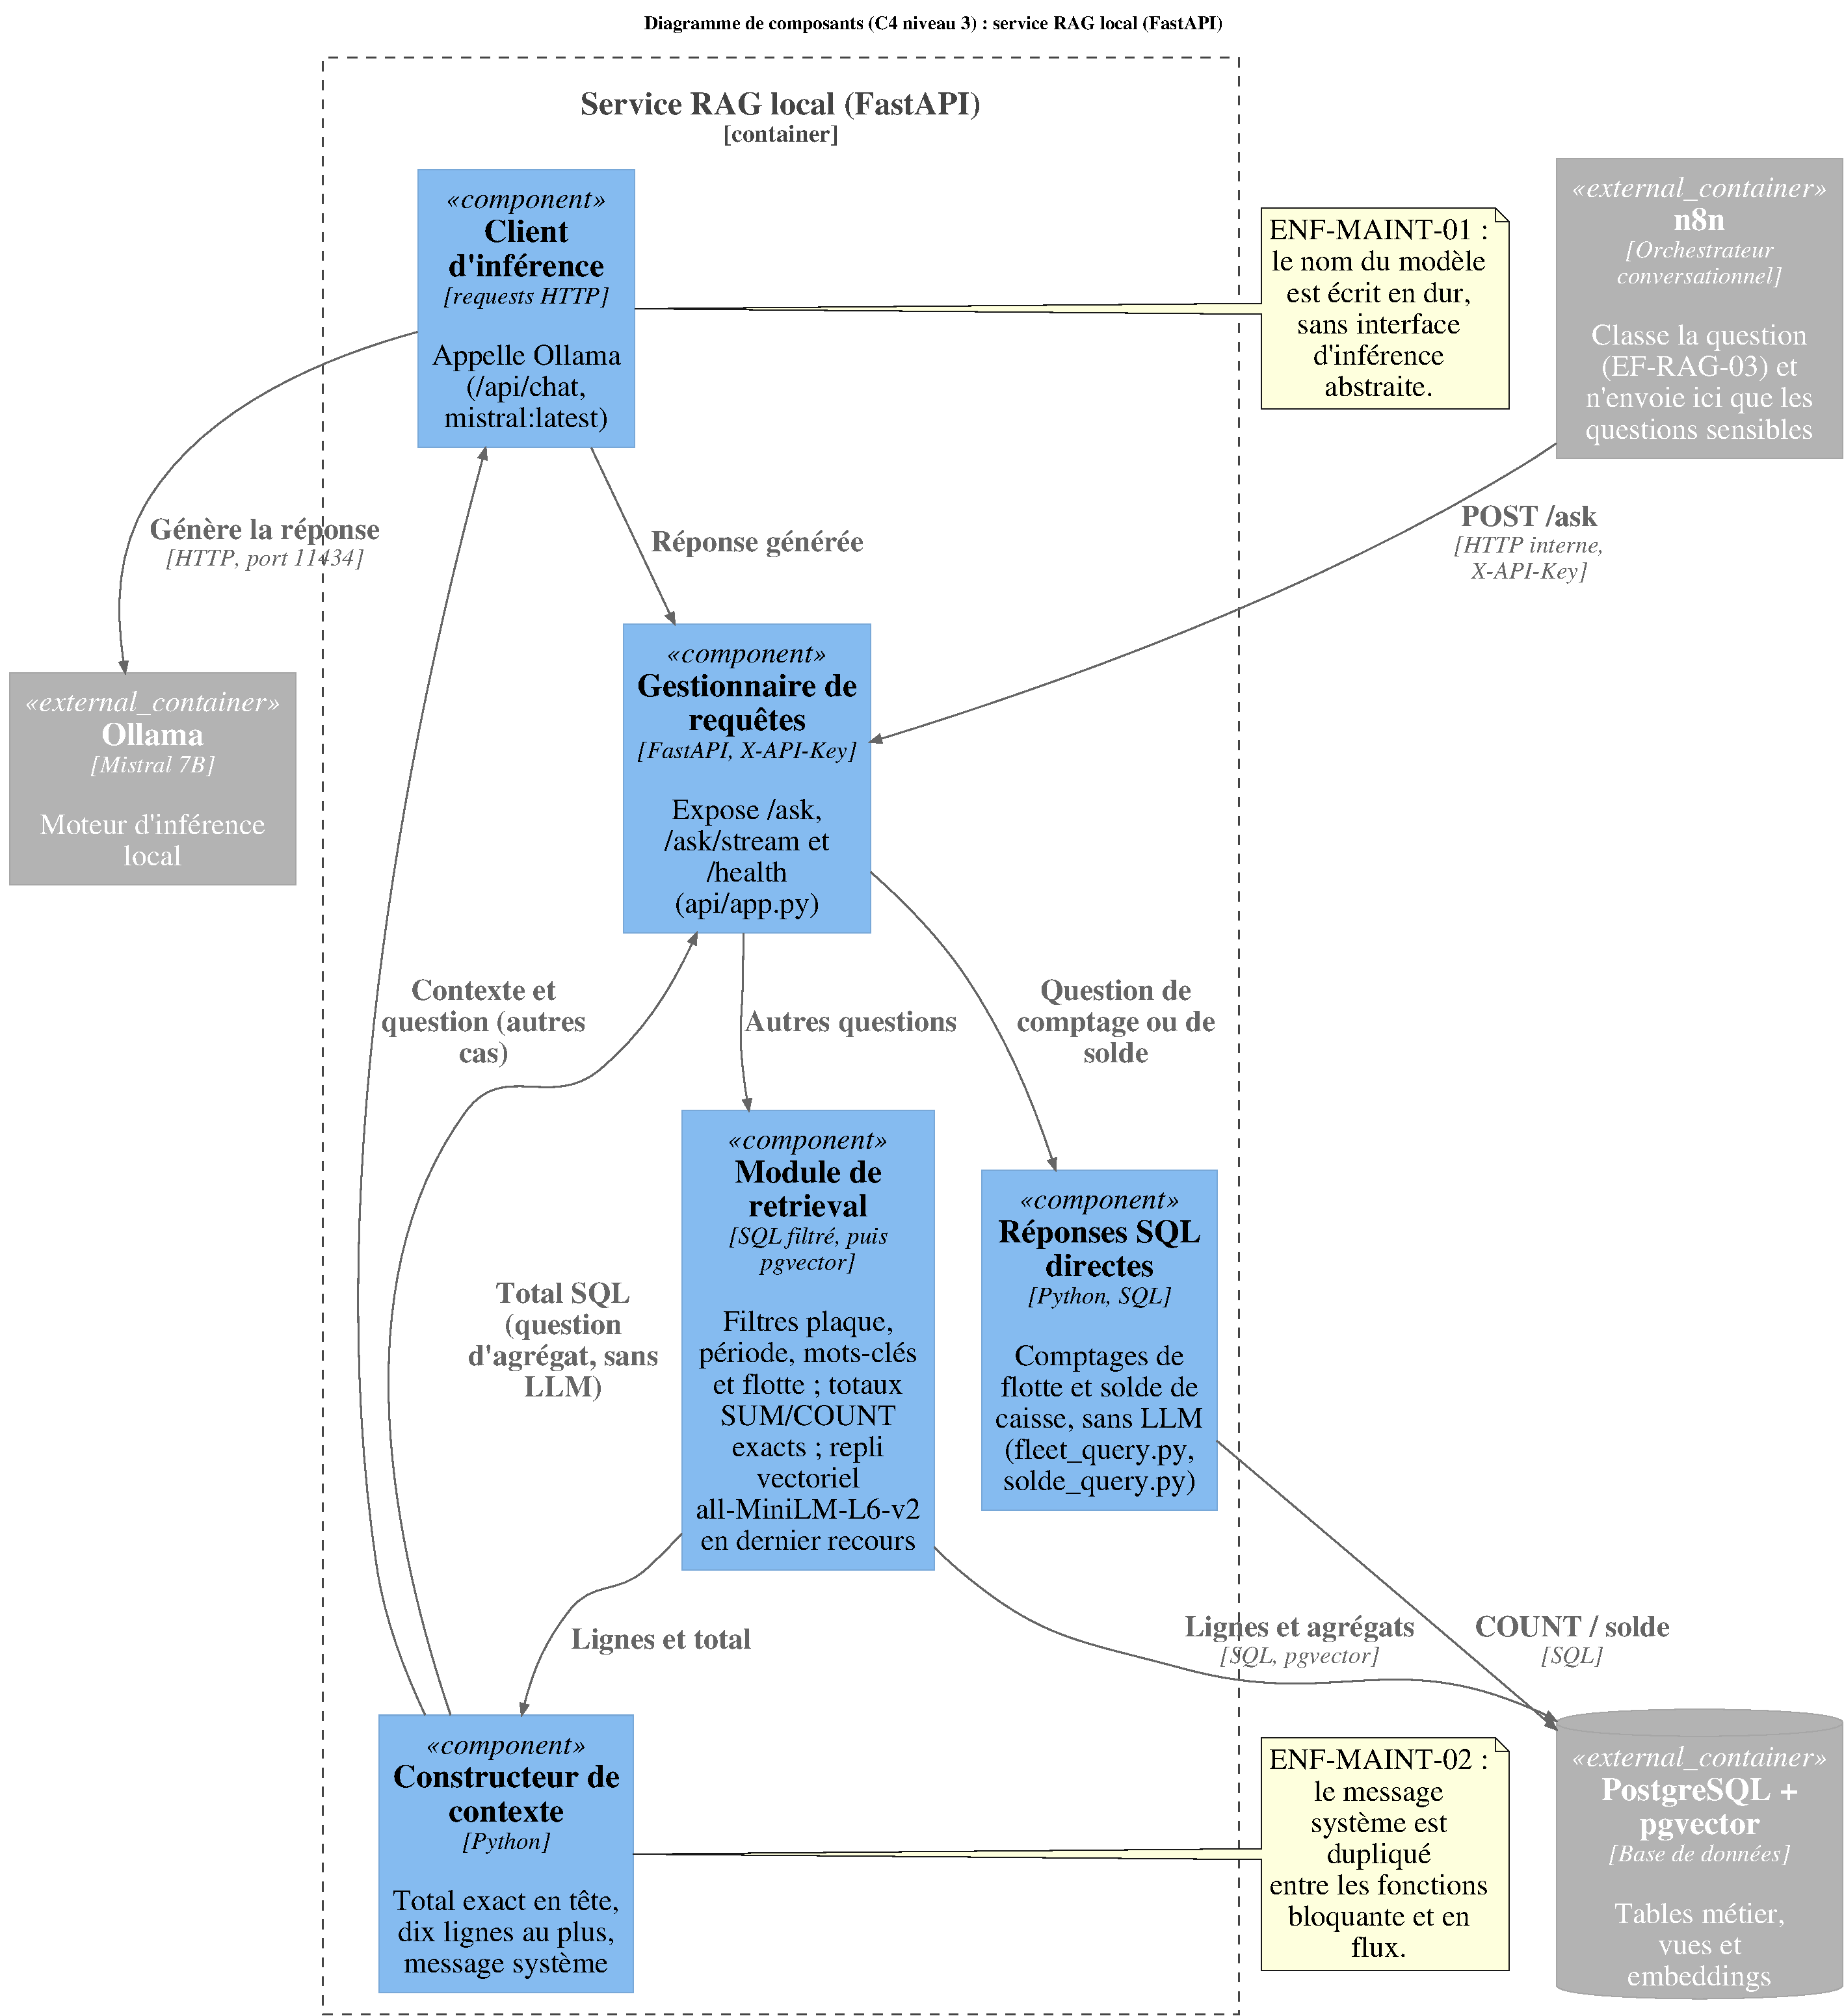
\includegraphics[width=\textwidth,height=0.88\textheight,keepaspectratio]{figures/fig_c4_composants_rag.pdf}
    \caption{Diagramme de composants (C4 niveau 3), service RAG local}
    \label{fig:c4_composants_rag}
    \source{Schéma de l'auteur}
\end{figure}

\subsection{Déploiement}
\label{sec:deploiement}
La Figure~\ref{fig:deploiement} décrit l'infrastructure de production : tous les conteneurs applicatifs, IA, ETL et de supervision sont hébergés sur un seul serveur dédié, ce qui soutient directement l'hypothèse de frugalité H1 (\texttt{ENF-FRUG-01}). Le trafic des clients passe par Cloudflare, chiffré de bout en bout (ADR-05). Quatre services externes complètent le schéma : l'API Anthropic pour le chemin cloud, GitLab.com pour les dépôts et les pipelines, Telegram pour les alertes et l'espace de sauvegarde de l'hébergeur. Pour rester lisible, le schéma est présenté en deux vues : la vue d'ensemble du serveur et de ses flux externes (Figure~\ref{fig:deploiement}), puis le détail des conteneurs du réseau Docker (Figure~\ref{fig:deploiement_docker}).

\begin{landscape}
\begin{figure}[p]
    \centering
    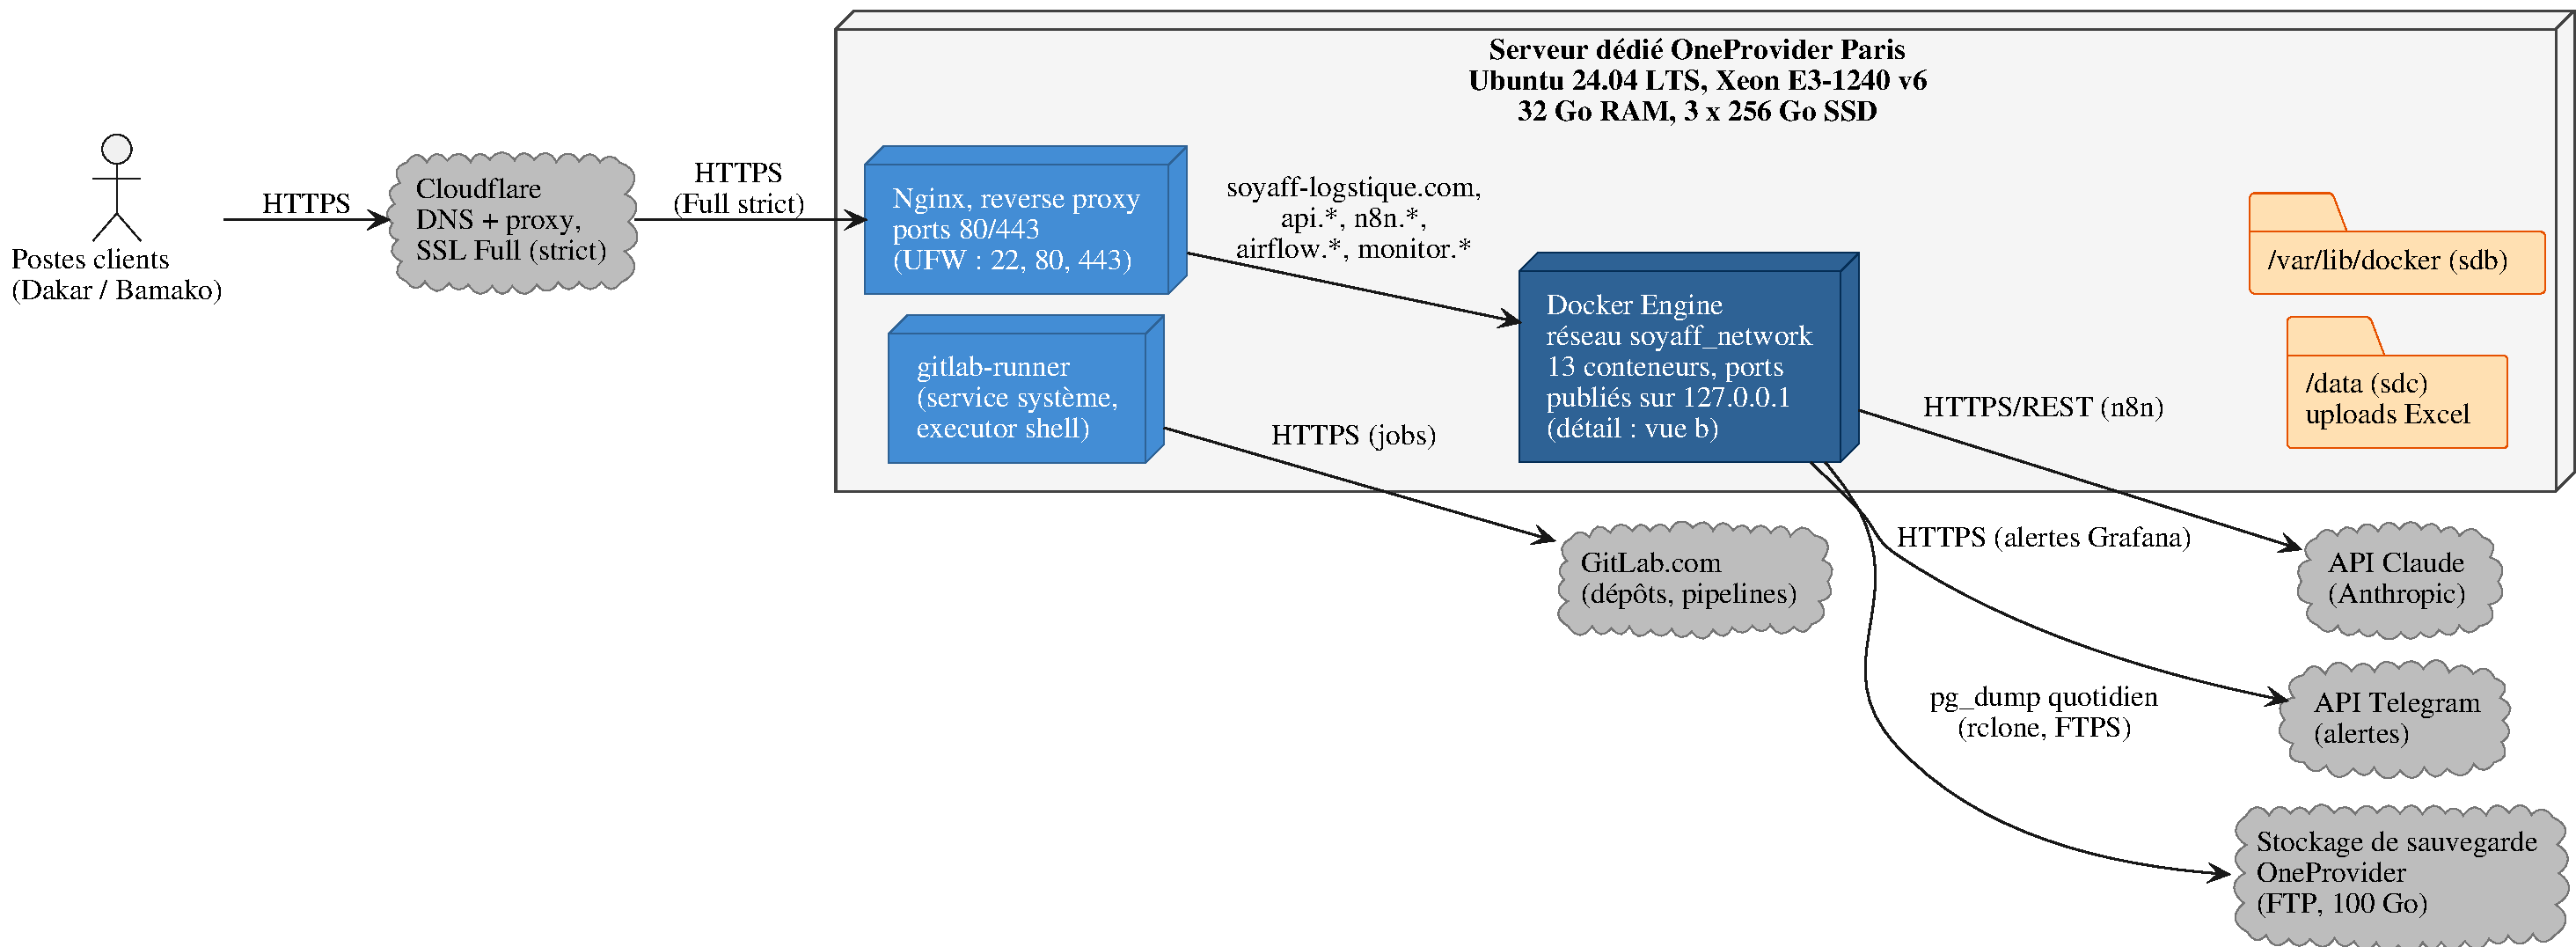
\includegraphics[width=\linewidth,height=0.86\textheight,keepaspectratio]{figures/fig_deploiement_vue.pdf}
    \caption{Diagramme de déploiement (1/2) : serveur de production et services externes}
    \label{fig:deploiement}
    \source{Schéma de l'auteur}
\end{figure}
\begin{figure}[p]
    \centering
    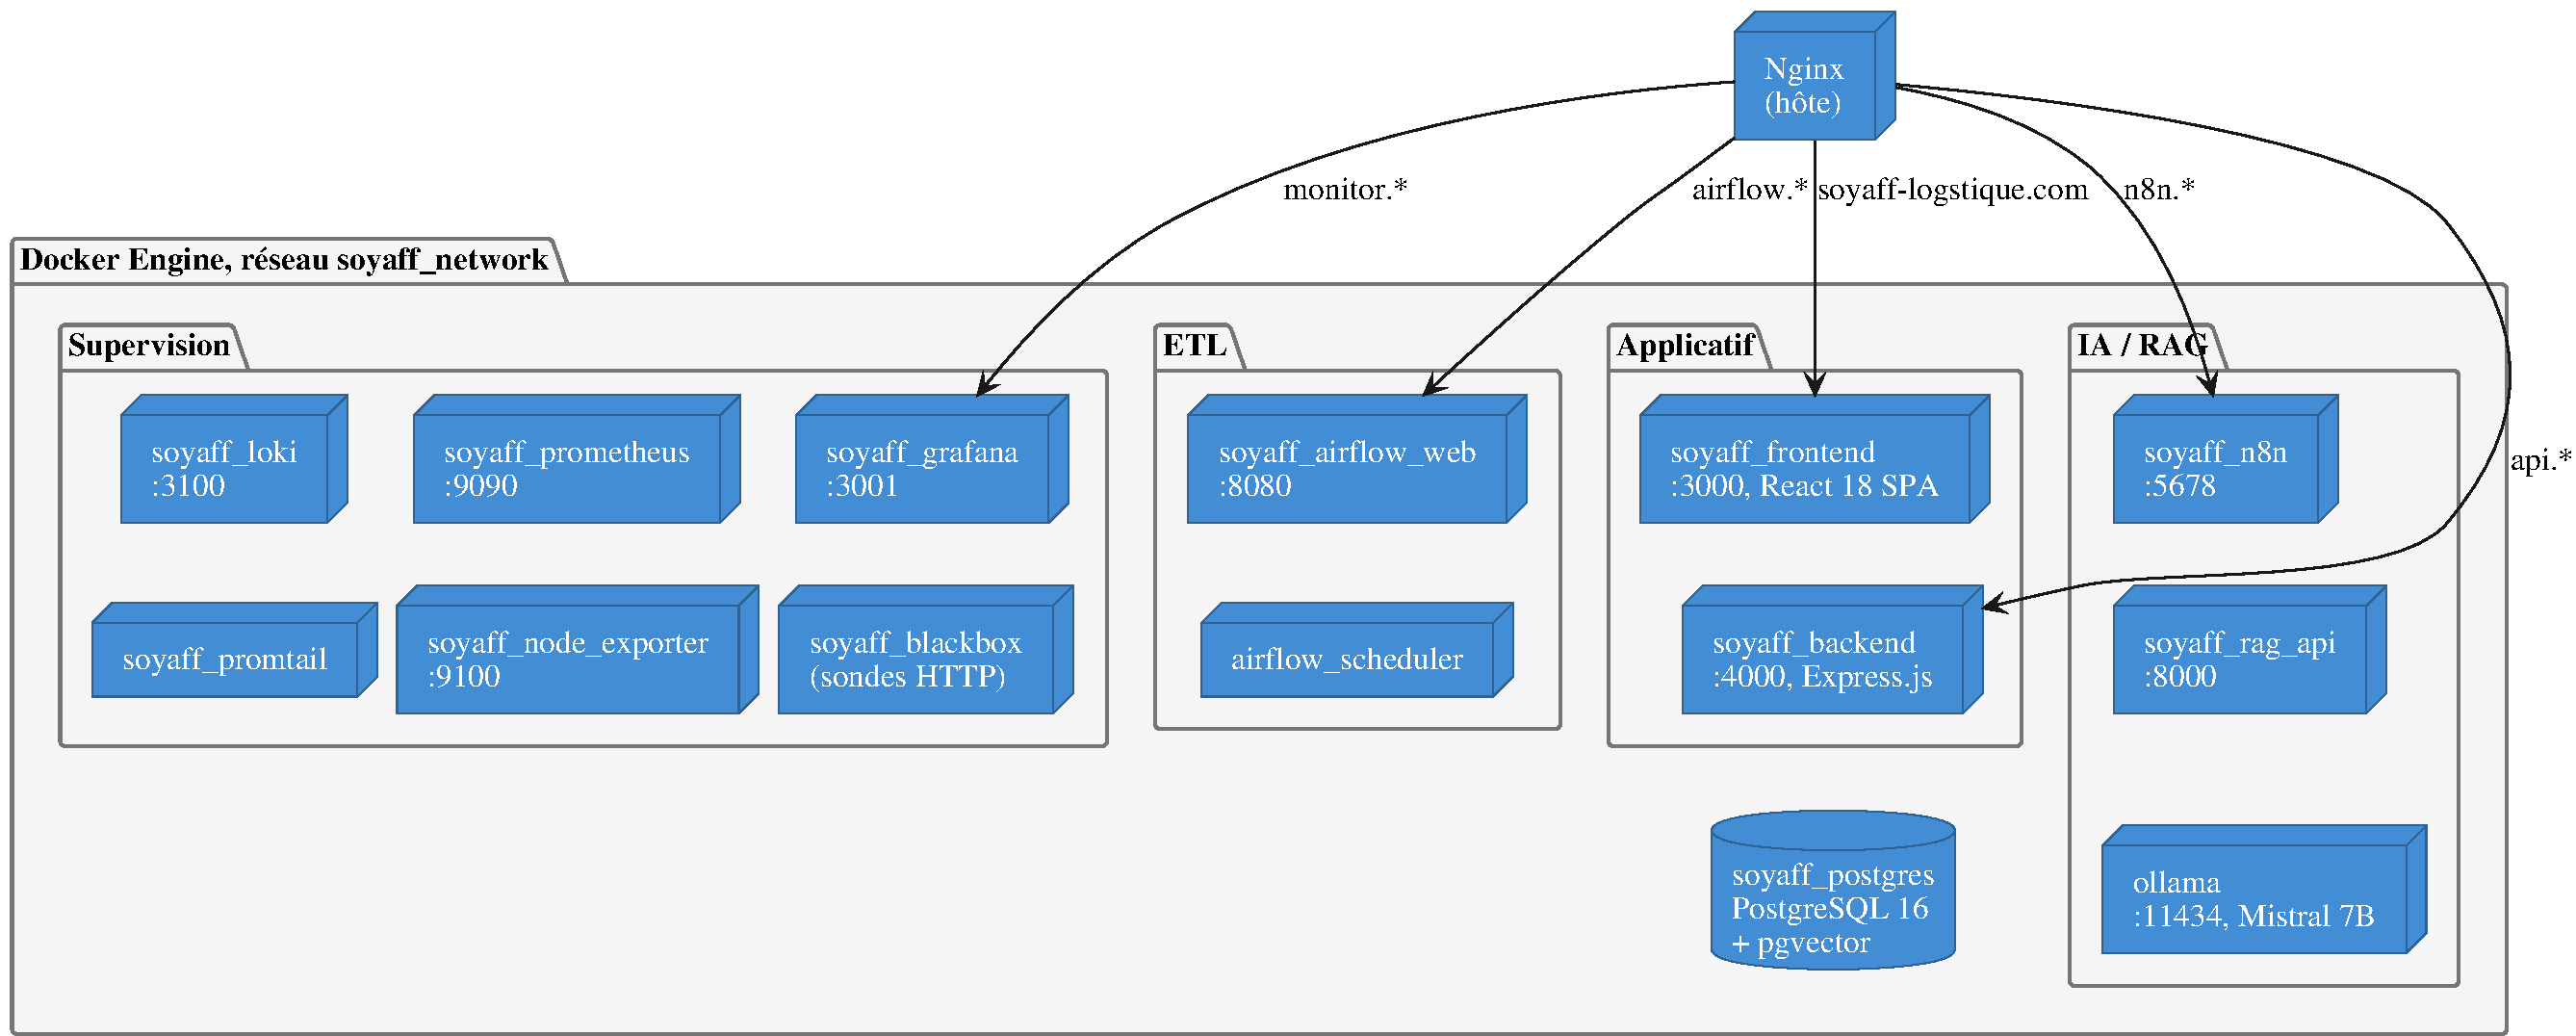
\includegraphics[width=\linewidth,height=0.86\textheight,keepaspectratio]{figures/fig_deploiement_docker.pdf}
    \caption{Diagramme de déploiement (2/2) : conteneurs du réseau Docker \texttt{soyaff\_network}}
    \label{fig:deploiement_docker}
    \source{Schéma de l'auteur}
\end{figure}
\end{landscape}

\subsection{Registre des décisions architecturales (ADR)}
\label{sec:adr}
Les vues précédentes décrivent l'architecture retenue. Cette section en justifie les décisions sous forme d'Architecture Decision Records (ADR) : contexte, option retenue, conséquences (bénéfices comme dettes assumées), et alternatives écartées.

\subsubsection*{ADR-01 : Orchestration ETL par Apache Airflow}
\textbf{Contexte.} Le pipeline d'ingestion des fichiers Excel hétérogènes (\texttt{RECAP-MENSUEL}, \texttt{RECAP-JOURNALIERE}) exige planification, idempotence et gestion de \textit{backfill} en environnement à connectivité intermittente, propre au corridor Dakar--Bamako (§2.2.3). Le choix de l'orchestrateur devait concilier maturité technique et indépendance vis-à-vis des éditeurs commerciaux (§2.2.4).

\textbf{Décision.} Apache Airflow est retenu comme orchestrateur ETL, modélisant le pipeline sous forme de DAG Python idempotents, la déduplication reposant sur la clé \texttt{source\_key} (\texttt{ON CONFLICT DO NOTHING}).

\textbf{Conséquences.} \textit{Positives} : licence Apache~2.0 garantissant une indépendance totale vis-à-vis d'un éditeur ; large éventail de connecteurs matures pour sources hétérogènes (Excel, PDF, PostgreSQL) ; gestion native du \textit{backfill}. \textit{Négatives} : courbe d'apprentissage modérée à difficile ; empreinte ressources plus lourde qu'un ordonnanceur léger de type \textit{cron}.

\textbf{Alternatives écartées.} Prefect et Dagster, tous deux adossés à un modèle commercial cloud qui réintroduirait précisément la dépendance logicielle exogène que l'architecture cherche à éviter (§2.2.4).

\textbf{Exigences / hypothèses liées.} \texttt{EF-ETL-01}, \texttt{EF-ETL-02}, \texttt{ENF-VOL-01}, H4.

\subsubsection*{ADR-02 : Routage hybride cloud/local par sensibilité}
\textbf{Contexte.} Une tension oppose la souveraineté des données sensibles (identités des chauffeurs, montants, opérations financières) à la puissance de calcul disponible localement pour l'inférence LLM, le serveur ne disposant d'aucun GPU dédié (§2.4). Le besoin décisionnel exprimé par \texttt{EF-RAG-01/02} exige néanmoins un agent conversationnel capable de traiter des requêtes analytiques complexes.

\textbf{Décision.} La sensibilité de chaque requête est classifiée en amont par un nœud d'analyse par mots-clés au sein du workflow n8n, qui route ensuite vers l'un de deux chemins : le service RAG local (FastAPI + pgvector + Ollama/Mistral, aucune sortie réseau) pour les requêtes sensibles, l'API Claude cloud pour les requêtes non sensibles.

\textbf{Conséquences.} \textit{Positives} : conformité déclarative à \texttt{ENF-SOUV-01} pour le périmètre classé sensible ; accès à la puissance d'un LLM cloud pour les requêtes complexes sans investissement GPU. \textit{Négatives} : la classification par mots-clés reste une heuristique et non un mécanisme certifié, avec un risque résiduel de faux négatif (requête sensible mal classée et routée vers le cloud) ; le chemin local ne repose pas encore sur une interface d'inférence abstraite (écart \texttt{ENF-MAINT-01}, §\ref{sec:c4_composants}). \textit{Résolu} (section~\ref{chap:ia_rag}, §\ref{sec:ia_routage}) : le workflow n8n est versionné et le routage a été vérifié dans les deux sens ; une mention d'identité (chauffeur, plaque) reste désormais locale même dans une question d'agrégat ; l'outil SQL de l'agent cloud utilise un rôle PostgreSQL en lecture seule, sans accès aux données des chauffeurs.

\textbf{Alternatives écartées.} Tout-cloud, écarté comme incompatible avec \texttt{ENF-SOUV-01} et H2 ; tout-local, écarté faute de puissance suffisante pour satisfaire \texttt{ENF-PERF-02/03} sur les requêtes analytiques complexes avec le matériel disponible.

\textbf{Exigences / hypothèses liées.} \texttt{EF-RAG-01} à \texttt{05}, \texttt{ENF-SOUV-01}, \texttt{ENF-SOUV-02}, H2.

\subsubsection*{ADR-03 : Déploiement mono-hôte sur serveur dédié unique}
\textbf{Contexte.} La contrainte budgétaire d'une PME subsaharienne (H1) doit être mise en balance avec le nombre croissant de services nécessaires à la plateforme (applicatif, IA, ETL, observabilité, CI/CD).

\textbf{Décision.} L'intégralité de la plateforme (quatorze conteneurs Docker) est hébergée sur un unique serveur dédié (OneProvider Paris, Xeon E3-1240 v6, 32~Go RAM, 3~$\times$~256~Go SSD), orchestrés via Docker Engine sur un réseau applicatif unique (\texttt{soyaff\_network}).

\textbf{Conséquences.} \textit{Positives} : coût d'infrastructure minimal, compatible avec \texttt{ENF-FRUG-01} ; simplicité opérationnelle d'un point d'administration unique. \textit{Négatives} : point de défaillance unique (\textit{SPOF}), donc aucune haute disponibilité : une panne matérielle ou une saturation de ressource affecte simultanément l'ensemble des services ; absence de scalabilité horizontale native. Cette dette est assumée explicitement et reprise à la section~\ref{chap:discussion}.

\textbf{Alternatives écartées.} Déploiement multi-nœuds ou infrastructure managée (Kubernetes cloud, bases de données managées), au coût mensuel incompatible avec \texttt{ENF-FRUG-01} et la réalité budgétaire d'une PME du secteur.

\textbf{Exigences / hypothèses liées.} \texttt{ENF-FRUG-01}, \texttt{ENF-DISP-02}, H1.

\subsubsection*{ADR-04 : PostgreSQL + pgvector plutôt qu'une base vectorielle dédiée}
\textbf{Contexte.} Le RAG local requiert un stockage d'embeddings vectoriels pour la recherche par similarité, en complément du stockage relationnel déjà nécessaire aux données métier (transactions, camions, chauffeurs).

\textbf{Décision.} Le stockage relationnel et vectoriel est mutualisé au sein d'un unique moteur PostgreSQL~16 étendu par \texttt{pgvector}, plutôt que de déployer une base vectorielle dédiée.

\textbf{Conséquences.} \textit{Positives} : un conteneur de moins à opérer et sécuriser, cohérent avec l'ADR-03 ; cohérence transactionnelle native entre données métier et embeddings, source de vérité unique facilitant la sauvegarde (\texttt{EF-ADM-03}) ; requêtes hybrides SQL/vectorielles en une seule transaction. \textit{Négatives} : performances de recherche vectorielle a priori inférieures à celles d'une base spécialisée sur de très gros volumes, ce qui n'est pas discriminant à la volumétrie actuelle de SOYAFF (\texttt{ENF-VOL-02}).

\textbf{Alternatives écartées.} Pinecone, écarté comme service SaaS propriétaire incompatible avec la souveraineté visée par H2 ; Qdrant ou Weaviate en conteneur dédié, fonctionnellement solides mais ajoutant un service supplémentaire à opérer sans bénéfice mesurable au volume actuel, à rebours de la frugalité visée par H1.

\textbf{Exigences / hypothèses liées.} \texttt{ENF-FRUG-01}, \texttt{ENF-SOUV-01}, \texttt{ENF-VOL-02}.

\subsubsection*{ADR-05 : Terminaison TLS Cloudflare (« Flexible », révisée en « Full (strict) »)}
\textbf{Contexte.} La mise en production rapide de la plateforme devait garantir un chiffrement du trafic client sans mobiliser de temps d'ingénierie supplémentaire pour la gestion de certificats sur le serveur.

\textbf{Décision.} Le mode SSL «\,Flexible\,» de Cloudflare avait d'abord été activé : il chiffrait le trajet poste client~$\rightarrow$~Cloudflare, mais laissait le trajet Cloudflare~$\rightarrow$~origine (serveur) en HTTP.

\textbf{Conséquences.} \textit{Positive} : mise en place immédiate, sans gestion de certificat côté serveur. \textit{Négative} : le trajet Cloudflare~$\rightarrow$~origine restait en clair, ce qui constituait un écart non conforme à \texttt{ENF-SEC-05} (chiffrement de bout en bout). Cette configuration a été traitée comme une dette technique assumée plutôt que comme un choix définitif.

\textbf{Alternatives écartées.} Mode Cloudflare «\,Full (strict)\,» avec certificat installé sur le serveur, écarté au départ pour des raisons de délai de mise en production.

\textbf{Révision (26~septembre~2026).} Le mode «\,Full (strict)\,» est désormais actif : le trajet Cloudflare~$\rightarrow$~origine est chiffré et le certificat du serveur est vérifié (§\ref{sec:devops_securite}). L'écart à \texttt{ENF-SEC-05} est refermé.

\textbf{Exigences / hypothèses liées.} \texttt{ENF-SEC-05}.

Cette section a posé l'architecture : quatre vues C4 et cinq décisions structurantes tracées en ADR, qui referment la conception ouverte par l'analyse des besoins. Chaque choix reste relié à une exigence, et in fine à une hypothèse de recherche. Les écarts entre conception et implémentation (interface d'inférence non abstraite, par exemple) sont des dettes assumées, reprises à la section~\ref{chap:discussion}. La Partie~III traduit maintenant ce plan en système opérationnel : pipeline d'ingestion, application web, module d'IA, infrastructure DevOps.



% ===== PARTIE III : MISE EN ŒUVRE =====
\part{Mise en œuvre}

\chapter{Réalisation de la solution}
\label{chap:realisation}

Ce chapitre décrit la mise en œuvre de la plateforme, brique par brique. Pour chacune, nous indiquons ce que nous avons déployé et une capture en apporte la preuve. Les captures établissent l'existence et le fonctionnement du système ; sa valeur est mesurée au chapitre~\ref{chap:evaluation}. La configuration détaillée figure en annexe~\ref{annexe:deploiement}.

\section{Environnement de réalisation}
\label{sec:env_realisation}

Nous avons déployé toute la plateforme sur un seul serveur dédié, loué chez OneProvider à Paris (ADR-03, \S\ref{sec:adr}). Le tableau~\ref{tab:env_serveur} en donne les caractéristiques et la Figure~\ref{fig:real_serveur} montre la configuration retenue à la commande.

\begin{table}[H]
\centering
\footnotesize
\caption{Caractéristiques du serveur de production}
\label{tab:env_serveur}
\begin{tabularx}{0.85\linewidth}{|l|X|}
\hline
\rowcolor[HTML]{EFEFEF}
\textbf{Élément} & \textbf{Valeur} \\ \hline
Hébergeur et localisation & OneProvider, Paris \\ \hline
Processeur & Intel Xeon E3-1240 v6, 4 cœurs / 8 threads, 3,7~GHz \\ \hline
Mémoire vive & 32~Go DDR3 \\ \hline
Stockage & 3~$\times$~256~Go SSD SATA \\ \hline
Réseau & 1~Gbit/s, trafic illimité \\ \hline
Sauvegarde externe & 100~Go (FTP), incluse dans l'offre \\ \hline
Système d'exploitation & Ubuntu 24.04 LTS \\ \hline
Coût & 30,23~USD/mois, sans frais d'installation \\ \hline
\end{tabularx}
\end{table}

\begin{figure}[H]
    \centering
    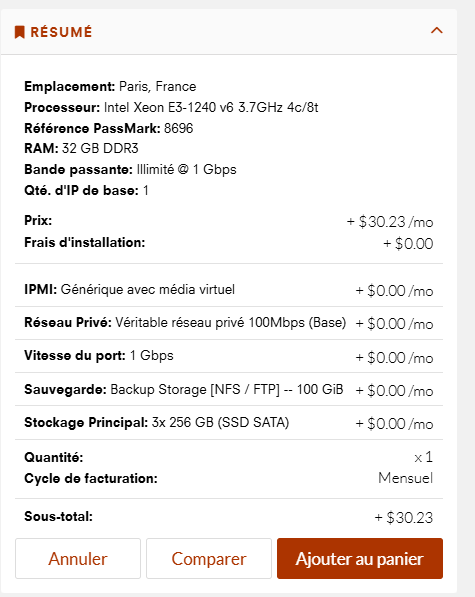
\includegraphics[width=0.5\textwidth]{figures/captures/real_serveur_offre.png}
    \caption{Configuration du serveur retenu à la commande}
    \label{fig:real_serveur}
\end{figure}

À l'installation du système, nous avons réservé le premier disque au système (\texttt{/boot}, 8~Go de \textit{swap}, racine). Les deux autres disques reçoivent les données Docker et les fichiers Excel importés (Figure~\ref{fig:real_partitionnement}). Un disque saturé par les images Docker ne bloque donc pas le système.

\begin{figure}[H]
    \centering
    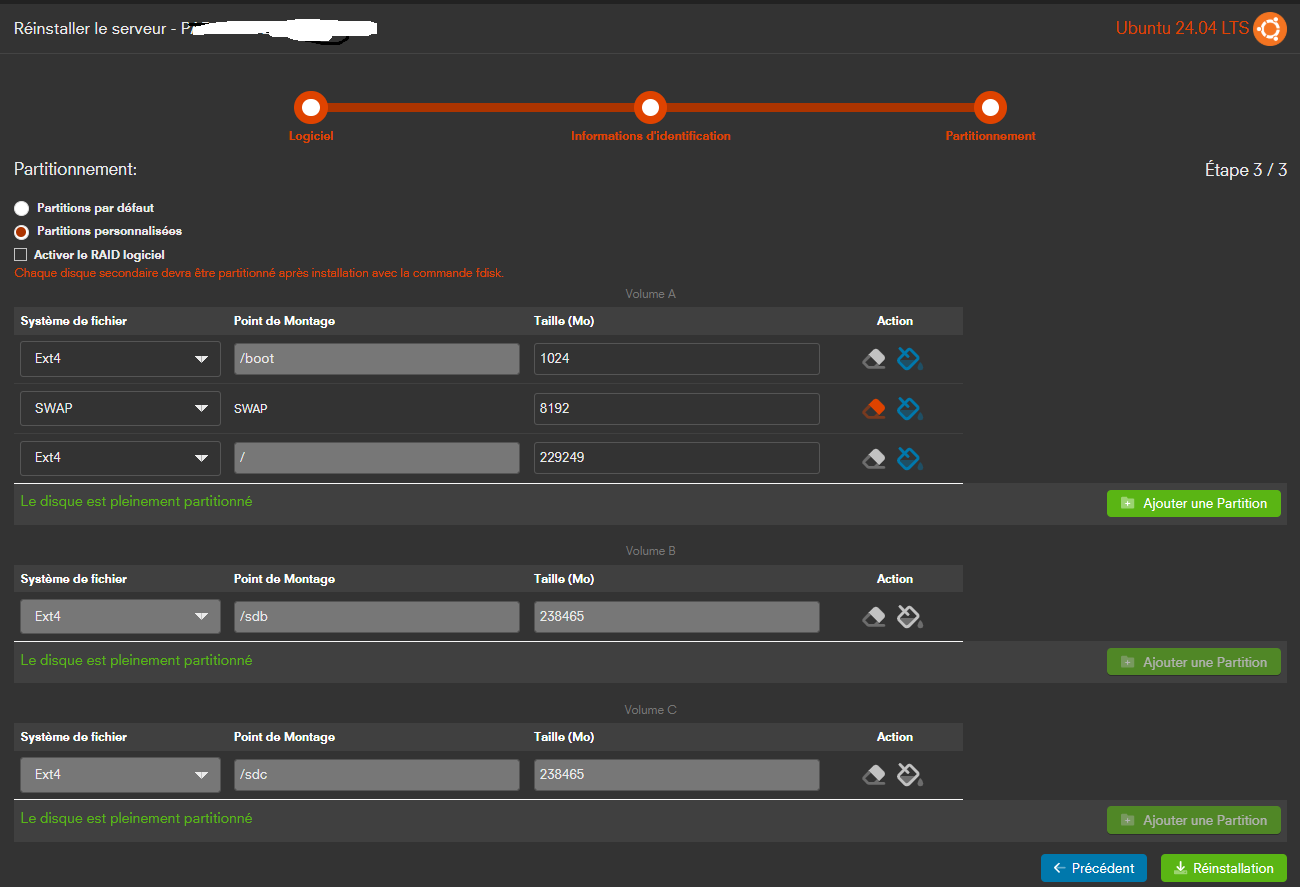
\includegraphics[width=0.85\textwidth]{figures/captures/real_partitionnement.png}
    \caption{Partitionnement des trois disques à l'installation d'Ubuntu 24.04 LTS}
    \label{fig:real_partitionnement}
\end{figure}

Le tableau~\ref{tab:env_versions} liste les composants logiciels en production et leur version, relevées directement sur le serveur. Les commandes de relevé figurent en annexe~\ref{annexe:deploiement}.

\begin{table}[H]
\centering
\footnotesize
\caption{Composants logiciels en production (relevé du 27~septembre~2026)}
\label{tab:env_versions}
\begin{tabularx}{\linewidth}{|l|X|l|}
\hline
\rowcolor[HTML]{EFEFEF}
\textbf{Composant} & \textbf{Rôle} & \textbf{Version} \\ \hline
Docker Engine / Compose & Conteneurisation et orchestration mono-hôte & 29.8.1 / 5.5.1 \\ \hline
PostgreSQL + pgvector & Base relationnelle et vectorielle & 16.15 / 0.8.6 \\ \hline
Apache Airflow & Orchestration du pipeline ETL & 2.7.3 \\ \hline
Python & Service RAG local (FastAPI) et ETL & 3.11.16 \\ \hline
Ollama / Mistral~7B & Inférence locale & 0.34.4 / 7B \\ \hline
n8n & Orchestration du routage hybride & 2.40.7 \\ \hline
Node.js & Backend Express & 20.20.2 \\ \hline
GitLab Runner & Exécution des pipelines CI/CD & 19.4.1 \\ \hline
\end{tabularx}
\end{table}

Le code est réparti en deux dépôts GitLab. Le premier, \texttt{assistant-soyaff}, porte le DAG Airflow, l'API RAG, le workflow n8n et les migrations de la base (Figure~\ref{fig:real_arbo_ia}). Le second, \texttt{assistant-soyaff-app}, porte le backend Express et le frontend React (Figure~\ref{fig:real_arbo_app}). Chaque dépôt a son propre pipeline de déploiement (\S\ref{sec:devops_cicd}).

\begin{figure}[H]
    \centering
    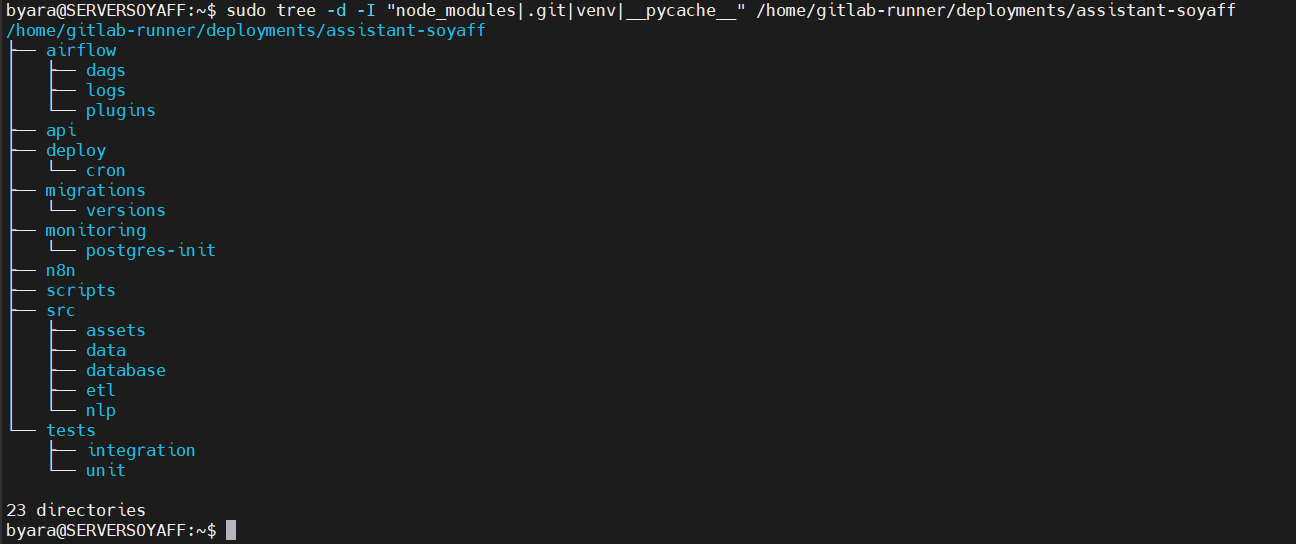
\includegraphics[width=0.75\textwidth]{figures/captures/real_arbo_ia.png}
    \caption{Arborescence du dépôt \texttt{assistant-soyaff} déployé sur le serveur}
    \label{fig:real_arbo_ia}
\end{figure}

\begin{figure}[H]
    \centering
    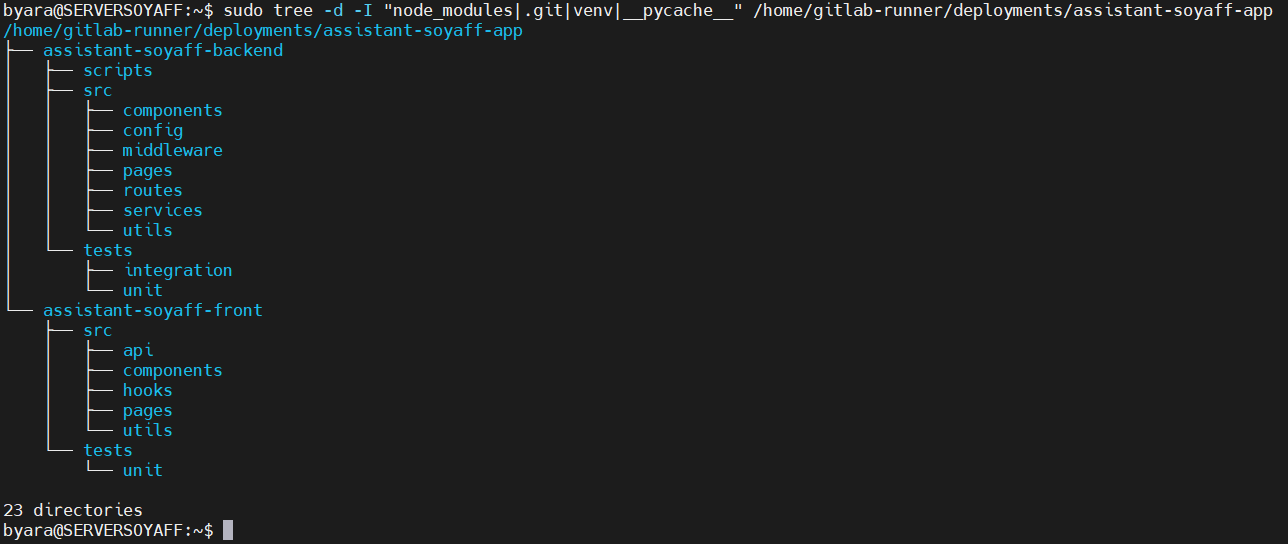
\includegraphics[width=0.75\textwidth]{figures/captures/real_arbo_app.png}
    \caption{Arborescence du dépôt \texttt{assistant-soyaff-app} déployé sur le serveur}
    \label{fig:real_arbo_app}
\end{figure}

\section{Pipeline ETL (Apache Airflow)}
\label{chap:etl}
Cette section décrit le pipeline qui alimente la plateforme à partir des fichiers tableurs historiques de SOYAFF. Il réalise les exigences \texttt{EF-ETL-01} (import de l'historique) et \texttt{EF-ETL-02} (absence de doublon), sous la contrainte de volume \texttt{ENF-VOL-01}. Le choix d'Airflow est justifié par l'ADR-01 (\S\ref{sec:adr}) ; nous nous concentrons ici sur les décisions imposées par la nature réelle des données.

\subsection{Architecture du pipeline et granularité d'orchestration}
\label{sec: architecture-pipeline}

Le DAG \texttt{etl\_excel\_to\_postgres} enchaîne deux tâches (Figure~\ref{fig:etl_dag}). La première, \texttt{run\_excel\_etl}, regroupe dans une seule fonction Python l'extraction, la transformation et le chargement. La seconde, \texttt{generate\_embeddings}, relit les transactions en base et calcule leurs vecteurs dans la table \texttt{transport\_embeddings}, hébergée dans la même instance PostgreSQL (ADR-04). Les deux tâches ne s'échangent aucune donnée en mémoire : leur seule frontière est l'état persisté en base.

\begin{figure}[H]
    \centering
    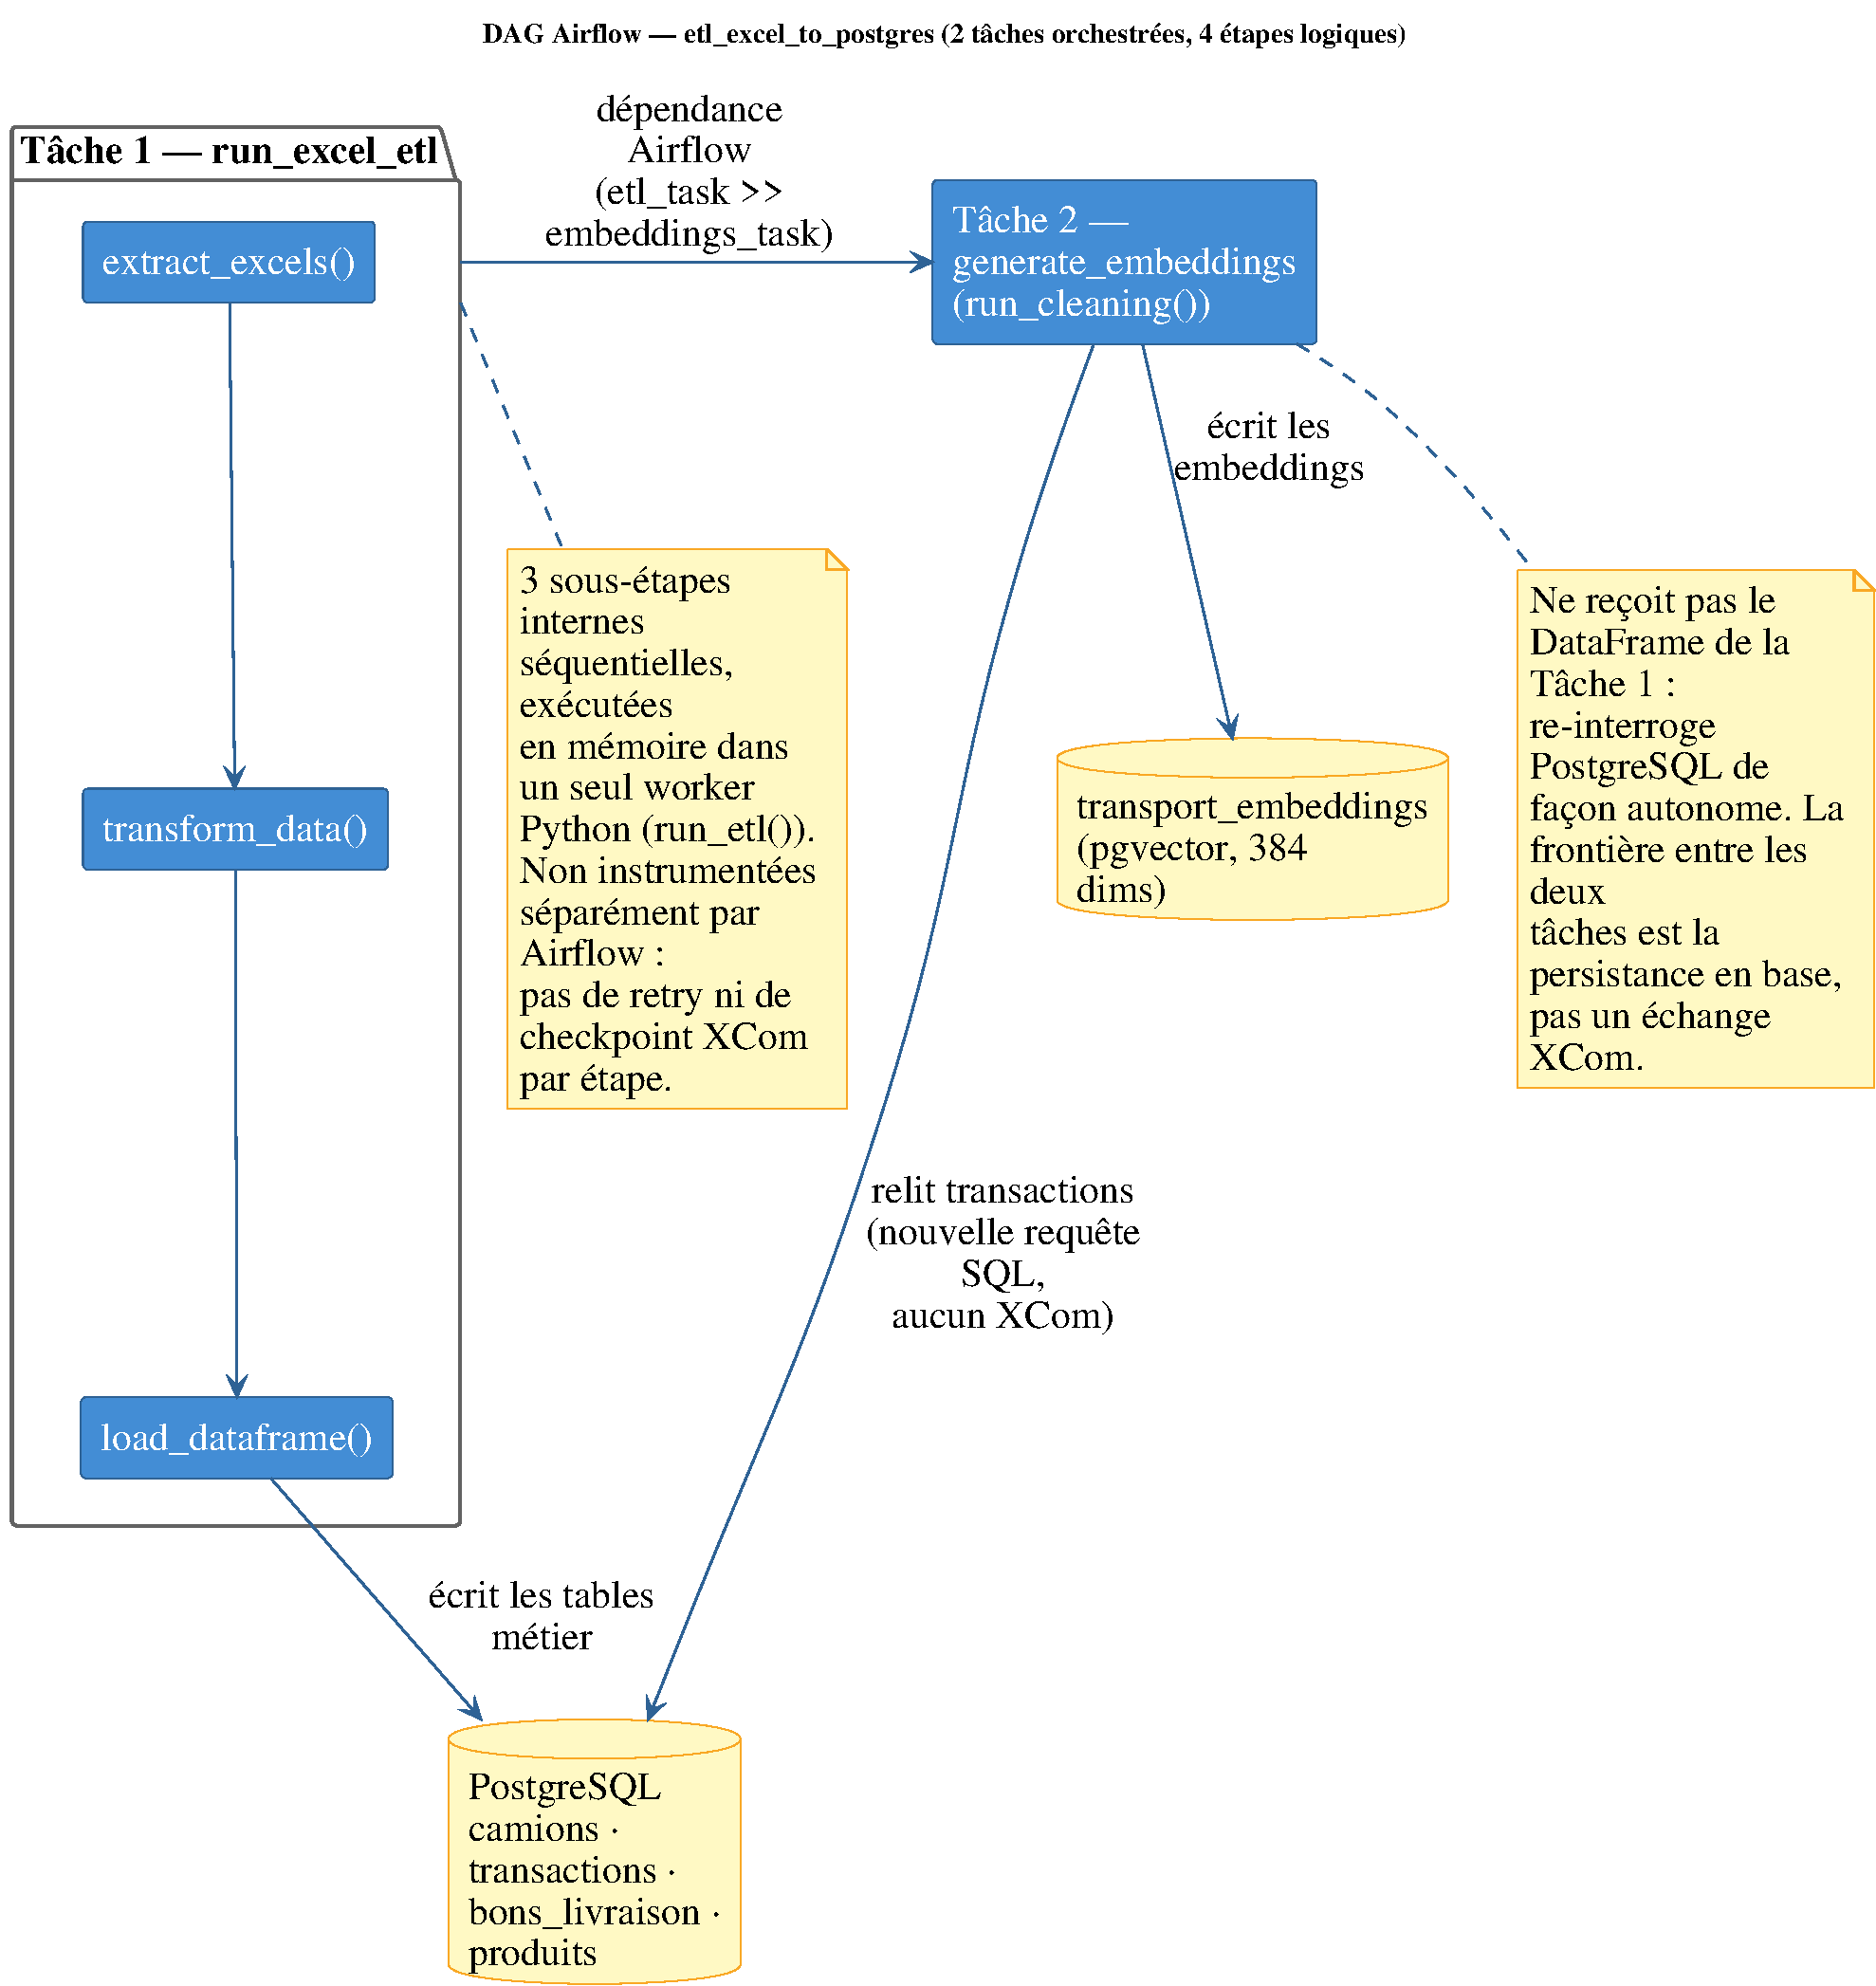
\includegraphics[width=\textwidth,height=0.88\textheight,keepaspectratio]{figures/fig_etl_dag.pdf}
    \caption{DAG Airflow \texttt{etl\_excel\_to\_postgres}, deux tâches orchestrées, quatre étapes logiques}
    \label{fig:etl_dag}
    \source{Schéma de l'auteur}
\end{figure}

\textbf{Pourquoi deux tâches, et pas quatre.} Découper extraction, transformation et chargement en trois tâches Airflow aurait obligé à faire transiter plusieurs milliers de lignes par \texttt{XCom}, un mécanisme qui n'est pas prévu pour ces volumes. Les regrouper garde les données en mémoire. Le prix est qu'un échec au chargement fait rejouer toute la tâche ; c'est sans danger, car l'extraction et la transformation sont rejouables à l'identique et le chargement est idempotent (\S\ref{sec: chargement}). La vectorisation, elle, est isolée pour une autre raison : c'est une charge de calcul, treize fois plus lente que le chargement (3~min~50 contre 17~s), qui mérite son propre suivi.

\textbf{Un déclenchement à la demande.} Les fichiers Excel contiennent des données personnelles : ils ne sont jamais versionnés, conformément à la loi n\textsuperscript{o}~2008-12 \cite{senegalLoi200812}. Un script transfère les fichiers vers le serveur par une liaison chiffrée, puis déclenche le DAG par l'API d'Airflow. Le DAG n'a donc pas de planification récurrente : il s'exécute à chaque dépôt de fichier.

\subsection{Extraction : absorber l'hétérogénéité des sources}
\label{sec: extraction}

L'informalité documentaire décrite dans l'état de l'art se lit dans chaque fichier. Les noms portent des doubles espaces ou un suffixe \texttt{- Copie} : aucune convention de nommage ne peut être présumée. Chaque feuille commence par une ligne de titre libre, suivie de deux lignes d'en-tête superposées. Les feuilles sont donc lues comme une grille brute, sans en-tête ; les noms de colonnes sont reconstitués à la transformation.

Les fichiers sont triés par ordre chronologique à partir du mois et de l'année lus dans leur nom. Un tri alphabétique placerait \textit{AOUT} avant \textit{AVRIL} et \textit{JANVIER}. Or la date d'émission d'un bon de livraison est fixée à sa première occurrence : sans ce tri, elle dépendrait de l'ordre des fichiers sur le disque, une corruption silencieuse. Chaque ligne est enfin étiquetée avec son fichier et sa feuille d'origine, pour l'audit et pour la clé de déduplication.

\subsection{Transformation et normalisation}
\label{sec: transformation}

\texttt{transform\_data()} impose un schéma unique en six étapes, chacune répondant à un défaut réel des classeurs :
\begin{enumerate}
    \item les deux lignes d'en-tête sont fusionnées en noms de colonnes (« Extrait » et « N° » deviennent \texttt{extrait\_n}) ;
    \item chaque colonne est reconnue par un motif sur son nom (\texttt{date}, \texttt{libell[eé]}, \texttt{camion}\ldots), et non par sa position, qui varie entre récapitulatifs mensuels et journaliers ; l'absence d'une colonne obligatoire arrête le traitement avec un message explicite ;
    \item les montants notés à la française (« 1.700.000 CFA ») sont convertis en nombres ;
    \item les dates sont lues au format jour/mois (\texttt{dayfirst=True}), sans quoi le 03/04 deviendrait le 4 mars ;
    \item les lignes « report solde », qui reportent un cumul d'une page à l'autre, sont écartées : elles fausseraient les totaux ;
    \item la clé de déduplication \texttt{source\_key} est calculée, après nettoyage, pour qu'un même montant écrit de deux façons produise la même clé.
\end{enumerate}

\subsection{Chargement idempotent}
\label{sec: chargement}

\textbf{La clé \texttt{source\_key}} est l'empreinte MD5 de neuf champs :
\[
\begin{aligned}
\texttt{source\_key} = \mathrm{MD5}\big(\;
  &\texttt{source\_file} \,\|\, \texttt{source\_sheet} \,\|\, \texttt{date\_transaction} \,\|\,{} \\
  &\texttt{libelle} \,\|\, \texttt{entrees\_appro} \,\|\, \texttt{sorties\_depenses} \,\|\,{} \\
  &\texttt{solde\_progressif} \,\|\, \texttt{camion\_raw} \,\|\, \texttt{bl\_raw}\;\big)
\end{aligned}
\]
Le fichier et la feuille séparent deux lignes identiques venues de mois différents ; le solde progressif, cumulatif, distingue deux lignes identiques d'un même fichier (plusieurs « CARBURANT GOLO » dans le mois). La colonne \texttt{source\_key} porte une contrainte d'unicité, et l'insertion utilise \texttt{ON CONFLICT (source\_key) DO NOTHING} : une ligne déjà présente est simplement comptée comme doublon. Rejouer le pipeline, entièrement ou en partie, n'insère donc aucun doublon ; c'est ce qui rend possible la reprise après une coupure de connexion (ADR-01).

\textbf{Des référentiels qui s'enrichissent.} Les tables \texttt{camions}, \texttt{bons\_livraison} et \texttt{produits} sont, elles, mises à jour à chaque import (\texttt{DO UPDATE}) : une transaction est un fait figé, un camion peut changer de statut. Un camion d'abord vu comme camion de la société peut être requalifié \texttt{particulier} par une « avance transport » ; l'inverse est interdit (Figure~\ref{fig:etl_table_camions}). Un libellé qui cite plusieurs camions est découpé et chaque camion est enregistré, mais seul le premier est rattaché à la transaction : c'est une limite du schéma. Une alerte signale les dépenses de carburant, de route, de ration ou d'amende sans camion identifié.

\begin{figure}[H]
    \centering
    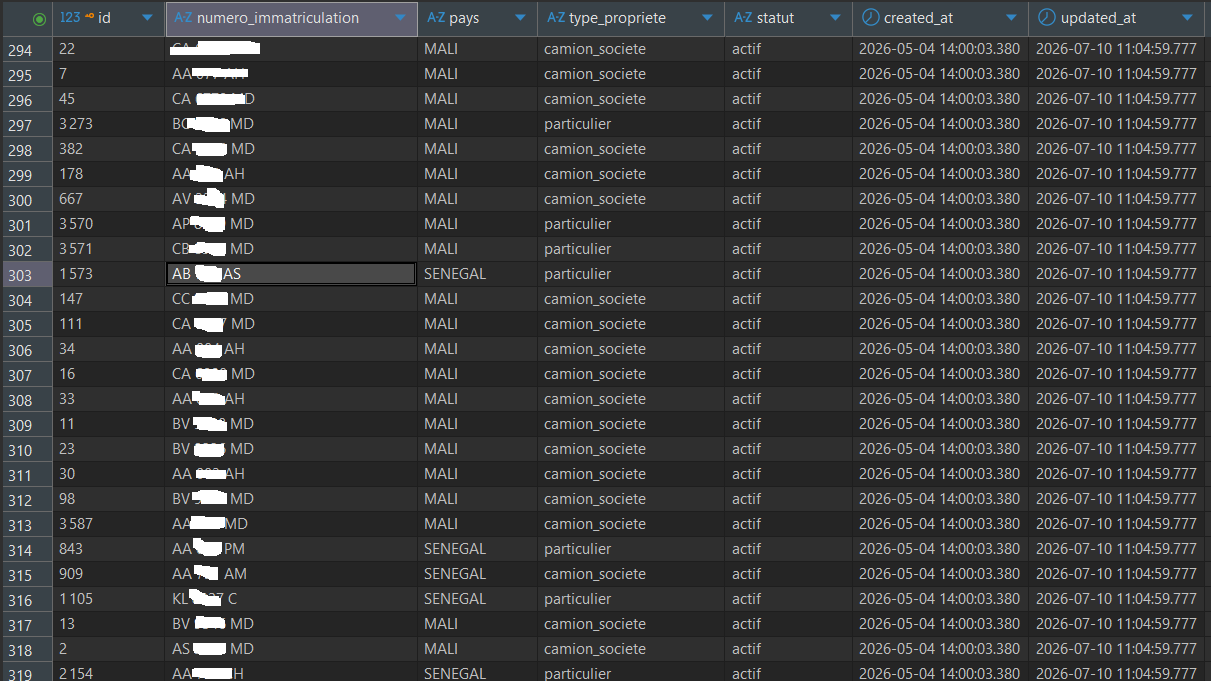
\includegraphics[width=0.8\textwidth]{figures/captures/etl_table_camions.png}
    \caption{Référentiel \texttt{camions} en base, classé par pays et type de propriété (extrait)}
    \label{fig:etl_table_camions}
\end{figure}

\begin{figure}[H]
    \centering
    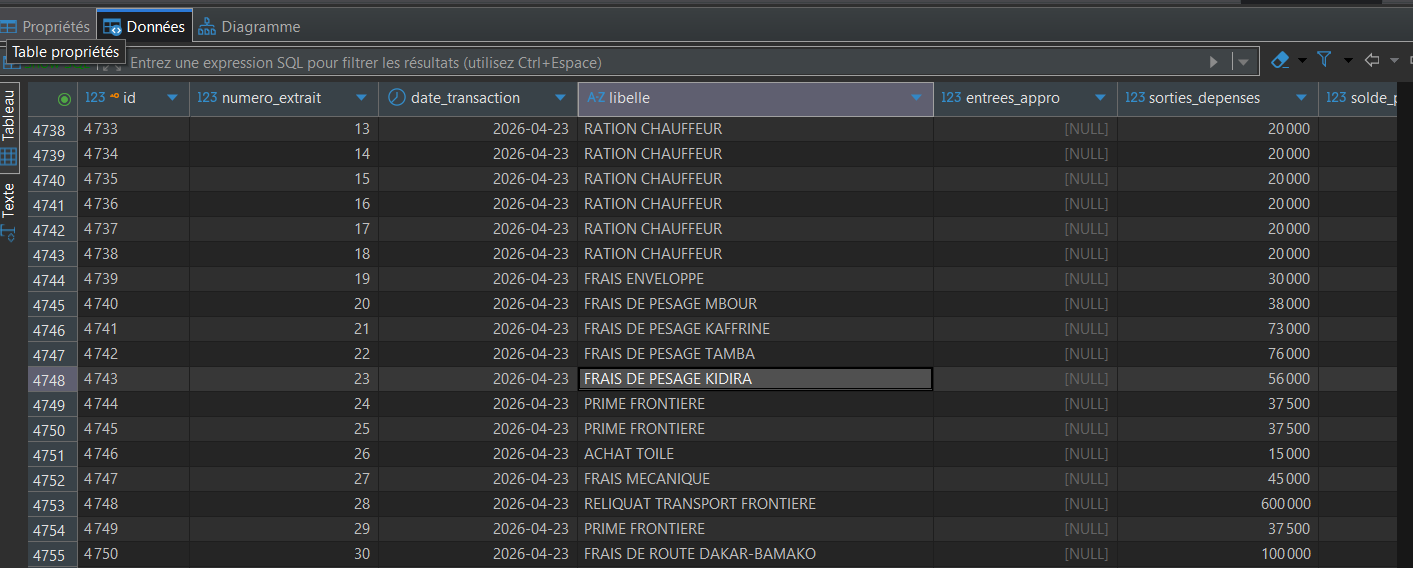
\includegraphics[width=0.8\textwidth]{figures/captures/etl_table_transactions.png}
    \caption{Transactions chargées dans PostgreSQL (extrait)}
    \label{fig:etl_table_transactions}
\end{figure}

\subsection{Vectorisation du batch ETL au corpus RAG}
\label{sec:  vectorisation}

La seconde tâche relit chaque transaction avec son camion, son bon de livraison et ses produits, compose un texte court (\textit{ex.} « Categorie carburant Camion AA~076~AH BL~1234 Produit gasoil »), puis le transforme en vecteur de 384 dimensions avec le modèle \texttt{all-MiniLM-L6-v2}. C'est le même modèle que celui qui encode les questions dans le service RAG local (\S\ref{sec:c4_composants}) : requêtes et corpus partagent le même espace. Les champs absents reçoivent une valeur explicite (\texttt{"inconnu"}) plutôt que la chaîne \texttt{"None"}. Les vecteurs sont enregistrés avec \texttt{ON CONFLICT (id) DO UPDATE} : rejouer la tâche rafraîchit les vecteurs sans les dupliquer (Figure~\ref{fig:etl_table_embeddings}).

\begin{figure}[H]
    \centering
    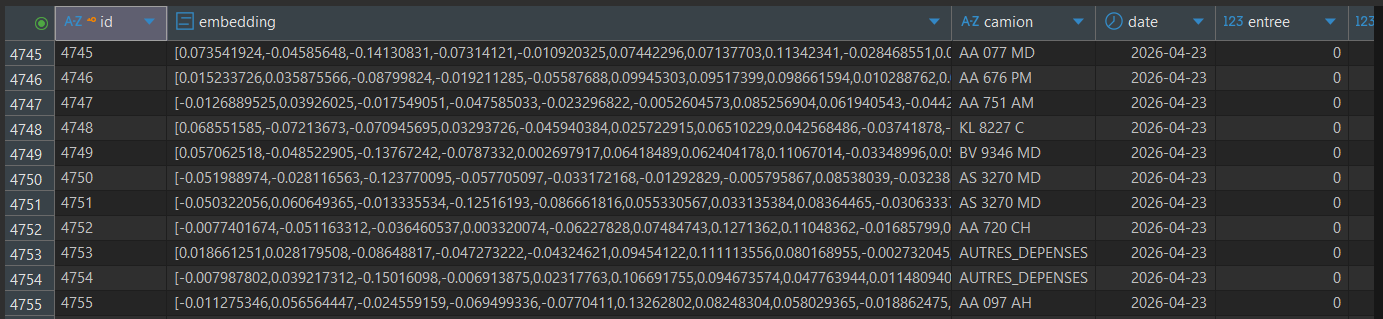
\includegraphics[width=0.8\textwidth]{figures/captures/etl_table_embeddings.png}
    \caption{Vecteurs d'embedding stockés dans \texttt{transport\_embeddings} (extrait)}
    \label{fig:etl_table_embeddings}
\end{figure}

\subsection{Validation du pipeline}
\label{sec: validation}

\textbf{Chargement initial.} Le 4~mai~2026, une exécution a ingéré 21 fichiers (15 récapitulatifs mensuels de janvier~2025 à mars~2026, 6 journaliers d'avril~2026). Elle a inséré 4~755 transactions, au-dessus du seuil de 4~500 de \texttt{ENF-VOL-01}. Les 3~595 enregistrements de camions correspondent à 319 camions distincts : un camion est compté à chaque apparition dans les transactions. Le Tableau~\ref{tab:validation_synthese} rassemble les chiffres.

\textbf{Preuve d'idempotence.} Le 10~juillet~2026, le même DAG a été relancé sur les mêmes fichiers, déjà chargés. Les deux tâches ont réussi (Figure~\ref{fig:etl_dag_rejeu}). Sur les 4~755 lignes, \textbf{4~755 ont été reconnues comme doublons et aucune n'a été insérée} (Figure~\ref{fig:etl_log_rejeu}). Les référentiels ont été mis à jour à l'identique. \texttt{EF-ETL-02} est ainsi démontrée par l'expérience, pas seulement par construction. La tâche de vectorisation compte 4~776 transactions : les 21 supplémentaires viennent de saisies de test faites dans l'application entre les deux dates (Figure~\ref{fig:etl_log_embeddings}).

\begin{figure}[H]
    \centering
    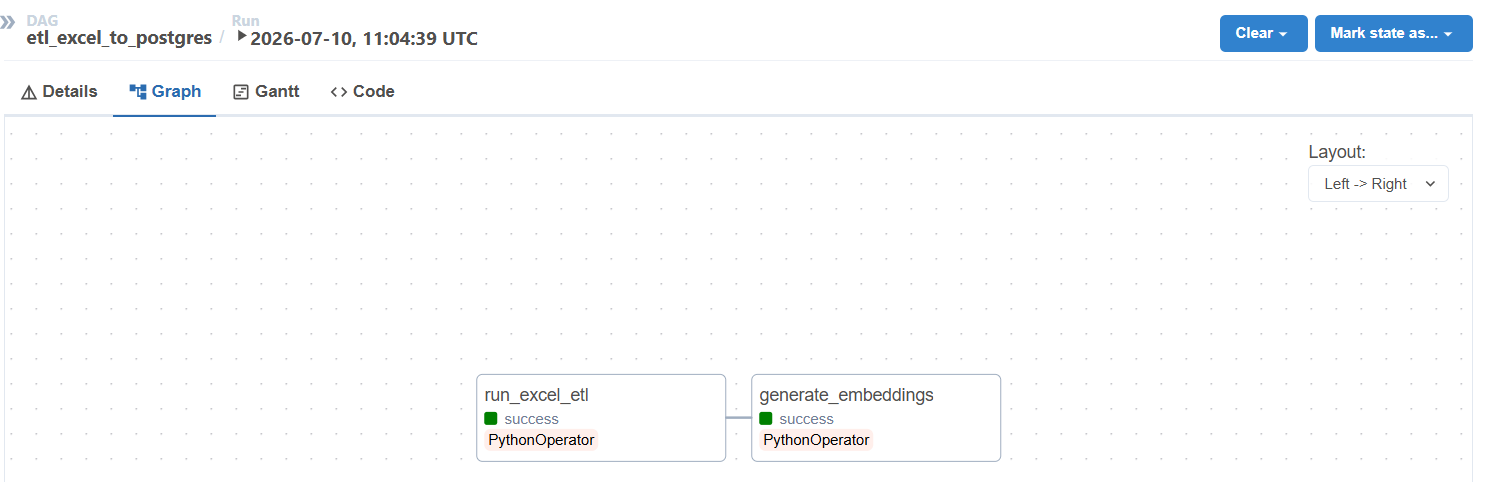
\includegraphics[width=0.8\textwidth]{figures/captures/etl_dag_rejeu.png}
    \caption{Rejeu de contrôle du 10~juillet~2026 dans Airflow : les deux tâches en succès}
    \label{fig:etl_dag_rejeu}
\end{figure}

\begin{figure}[H]
    \centering
    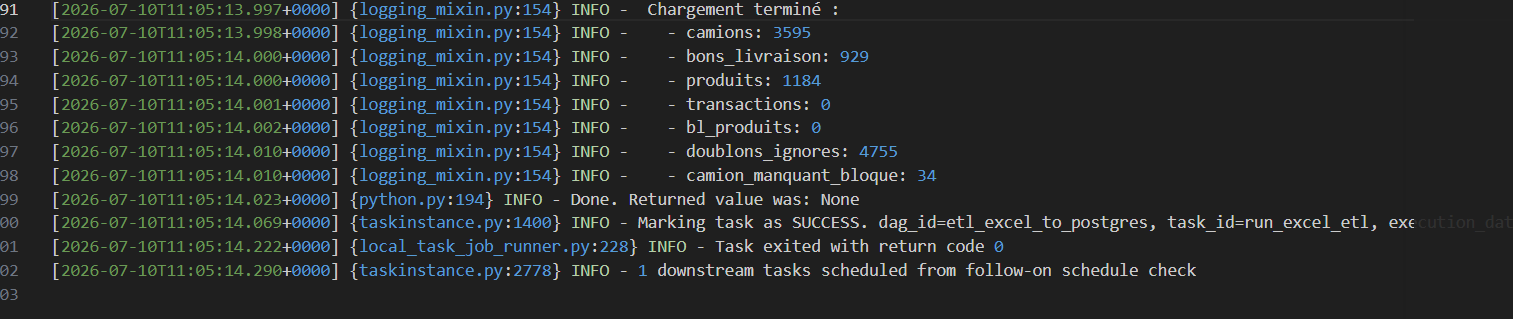
\includegraphics[width=0.95\textwidth]{figures/captures/etl_log_rejeu.png}
    \caption{Journal de la tâche \texttt{run\_excel\_etl} au rejeu : 0 transaction insérée, 4~755 doublons ignorés}
    \label{fig:etl_log_rejeu}
\end{figure}

\begin{figure}[H]
    \centering
    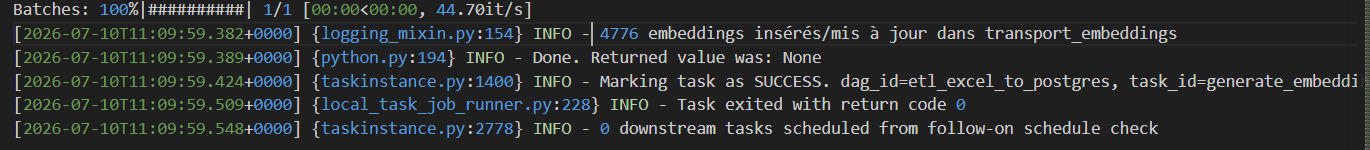
\includegraphics[width=0.95\textwidth]{figures/captures/etl_log_embeddings.png}
    \caption{Journal de la tâche \texttt{generate\_embeddings} au rejeu : 4~776 embeddings insérés ou mis à jour}
    \label{fig:etl_log_embeddings}
\end{figure}

\textbf{Rejets et durée.} L'extraction produit 5~023 lignes brutes ; 268 sont écartées (5,3~\%) : reports de solde, lignes sans date ou sans libellé, lignes de titre des fichiers suivant le premier. Le pipeline ne distingue pas ces causes : leur répartition n'est pas mesurée. Les 34 dépenses sans camion identifié sont chargées avec une alerte, pas rejetées. Le DAG complet s'exécute en moins de 4~min~35, ce qui permet un traitement après chaque dépôt de fichier.

\begin{table}[htbp]
\centering
\footnotesize
\caption{Validation du pipeline : chargement initial (04/05/2026) et rejeu de contrôle (10/07/2026)}
\label{tab:validation_synthese}
\begin{tabularx}{\linewidth}{|>{\raggedright\arraybackslash}X|>{\raggedright\arraybackslash}p{3.0cm}|>{\raggedright\arraybackslash}p{3.4cm}|}
\hline
\rowcolor[HTML]{EFEFEF}
\textbf{Métrique} & \textbf{Valeur mesurée} & \textbf{Exigence / statut} \\ \hline
Fichiers ingérés & 21 & \\ \hline
Transactions insérées & 4~755 & \texttt{ENF-VOL-01} ($\geq$~4~500) : dépassé \\ \hline
Camions : enregistrements / distincts & 3~595 / 319 & \\ \hline
Bons de livraison : enregistrements / distincts & 929 / 727 & \\ \hline
Produits : enregistrements / distincts & 1~184 / 633 & \\ \hline
Doublons reconnus au rejeu & 4~755 / 4~755 & \texttt{EF-ETL-02} : prouvé \\ \hline
Transactions insérées au rejeu & 0 & \texttt{EF-ETL-02} : prouvé \\ \hline
Lignes écartées & 268 / 5~023 (5,3~\%) & causes non ventilées \\ \hline
Dépenses sans camion identifié & 34 & chargées avec alerte \\ \hline
Durée : chargement / vectorisation / DAG & 17~s / 3~min~50 / 4~min~35 & \\ \hline
\end{tabularx}
\end{table}

\subsection{Synthèse et transition}
\label{sec: synthese-transition}

Le pipeline transforme des classeurs hétérogènes en une base relationnelle et vectorielle cohérente, qu'on peut rejouer sans risque. Il satisfait \texttt{EF-ETL-01}, \texttt{EF-ETL-02} et \texttt{ENF-VOL-01}. La section suivante décrit l'application web qui met ces données entre les mains des utilisateurs.

\section{Application web full-stack}
\label{chap:webapp}

L'application web expose aux utilisateurs de SOYAFF la base consolidée par le pipeline ETL (section~\ref{chap:etl}). Elle repose sur React~18 côté client et Express~4 côté serveur, avec une authentification par jetons signés et trois rôles. Le module conversationnel, bien que relayé par le même backend, est traité à part (section~\ref{chap:ia_rag}).

Les captures établissent que chaque fonctionnalité existe et fonctionne sur le système déployé ; leur valeur pour SOYAFF est mesurée au chapitre~\ref{chap:evaluation}. Le texte justifie les décisions qu'aucun écran ne montre. Le Tableau~\ref{tab:couverture_webapp} indique, exigence par exigence, ce qui tourne en production au 27~septembre~2026.

\begin{table}[htbp]
\centering
\footnotesize
\caption{Couverture des exigences applicatives par la réalisation (état au 27~septembre~2026)}
\label{tab:couverture_webapp}
\begin{tabularx}{\linewidth}{|>{\raggedright\arraybackslash}p{2.0cm}|>{\raggedright\arraybackslash}p{3.1cm}|>{\raggedright\arraybackslash}X|>{\raggedright\arraybackslash}p{1.5cm}|}
\hline
\rowcolor[HTML]{EFEFEF}
\textbf{Exigence} & \textbf{Fonctionnalité} & \textbf{Réalisation} & \textbf{État} \\ \hline

\texttt{EF-DSH-01} & Suivi de caisse en temps réel & \texttt{GET /api/stats} (lecture seule, agrégats parallèles) & \textbf{Déployé} \\ \hline
\texttt{EF-DSH-02}, \texttt{EF-DSH-04} & Visualisation de la flotte, profil véhicule & \texttt{CamionsPage.jsx} : liste, filtres, détail via \texttt{GET /api/camions} et \texttt{GET /api/camions/:id} & \textbf{Déployé} \\ \hline
\texttt{EF-DSH-03} & Classification société / particulier & Affichage typé (\texttt{type\_propriete}), bascule société~$\rightarrow$~particulier gérée à l'upsert & \textbf{Déployé} \\ \hline
\texttt{EF-SDR-01} & Saisie directe d'une opération financière & Page \texttt{SaisiePage.jsx} (\texttt{OperationForm.jsx}) $\rightarrow$ \texttt{POST /api/finances/operation} (transaction SQL atomique) & \textbf{Déployé} \\ \hline
\texttt{EF-SDR-02} & Contrôle des délais entre opérations d'un même camion & \texttt{utils/delais.js}, appliqué par l'API : frais de route bloqués sous 8~jours ; rations bloquées sous 2~jours, alerte à confirmer entre 2 et 5~jours ; forçage réservé à l'administrateur, tracé & \textbf{Déployé} \\ \hline
\texttt{EF-REP-01}, \texttt{EF-REP-02} & Récapitulatif journalier et mensuel consolidé & \texttt{GET /api/rapports/mois}, \texttt{GET /api/rapports/mensuel} & \textbf{Déployé} \\ \hline
\texttt{EF-REP-03} & Export CSV / Excel / PDF & CSV conforme Excel-FR (BOM~UTF-8, séparateur~\texttt{;}) et XLSX (\texttt{exceljs}) déployés ; PDF absent côté serveur, le bouton correspondant déclenche un \texttt{window.print()} navigateur & \textbf{Partiel} \\ \hline
\texttt{EF-REP-04} & Recherche multi-critères & Filtres période / camion / catégorie (\texttt{FinancesPage.jsx}, \texttt{RapportsPage.jsx}) & \textbf{Déployé} \\ \hline
\texttt{EF-VAL-02} & Workflow de validation numérique dématérialisé & Aucun statut de workflow en base ; insertion directe et définitive de la transaction & \textbf{Cible} \\ \hline
\texttt{EF-ADM-01} & Gestion des utilisateurs et des rôles & CRUD complet (\texttt{routes/admin.js}) : création, activation/désactivation, changement de rôle & \textbf{Déployé} \\ \hline
\texttt{EF-ADM-02} & Consultation des journaux d'audit & Onglet audit \texttt{AdminPage.jsx} $\rightarrow$ \texttt{GET /api/admin/audit}, table \texttt{audit\_logs} & \textbf{Déployé} \\ \hline
\texttt{ENF-SEC-01} & Authentification par jetons signés & JWT d'accès (8~h) + jeton de rafraîchissement (7~jours, haché SHA-256 en base) & \textbf{Déployé} \\ \hline
\texttt{ENF-SEC-02} & Hachage des mots de passe & \texttt{bcrypt}, coût~12 & \textbf{Déployé} \\ \hline
\texttt{ENF-SEC-03} & Contrôle d'accès basé sur les rôles & Contrainte \texttt{CHECK} SQL + middleware \texttt{authorize()} : \texttt{DAKAR\_AGENT}, \texttt{BAMAKO\_CHEF}, \texttt{ADMIN} & \textbf{Déployé} \\ \hline
\texttt{ENF-SEC-04} & Piste d'audit des actions sensibles & Table \texttt{audit\_logs} horodatée (connexions, refus d'accès, actions admin) & \textbf{Déployé} \\ \hline
\texttt{ENF-DISP-01} & Mode dégradé hors-ligne, cache local des saisies & Aucune trace de code (pas de \textit{service worker}, pas de file d'attente locale) & \textbf{Cible} \\ \hline
\end{tabularx}
\end{table}

Le socle de sécurité et le cœur métier (saisie, tableau de bord, reporting, administration) sont déployés et utilisés en production. Un point est partiel : l'export PDF, qui n'est qu'une impression du navigateur. Deux exigences \textit{Should} restent des cibles : le workflow de validation (\texttt{EF-VAL-02}) et le mode hors-ligne (\texttt{ENF-DISP-01}). La discussion de ces écarts est renvoyée à la section~\ref{chap:discussion}.

\subsection{Architecture applicative générale}
\label{sec:webapp_architecture}

La vue de conteneurs (Figure~\ref{fig:c4_conteneurs}) situe la pile : une \textit{single-page application} React~18 consomme une API REST Express~4 adossée à PostgreSQL. Deux choix d'organisation interne, invisibles sur les diagrammes, méritent d'être justifiés.

\textbf{Côté client, pas de routeur.} La vue affichée est portée par un simple état local dans \texttt{App.jsx}. Pour sept vues fixes, un routeur n'apportait rien. Le coût est double : aucune vue n'a d'URL propre, et la garde d'accès à l'administration est répétée au point de rendu au lieu d'être centralisée. Ce second point n'ouvre pas de faille : l'API vérifie elle-même le rôle (\S\ref{sec:webapp_rbac}), et contourner l'interface ne donnerait accès qu'à un écran vide.

\textbf{Côté serveur, le SQL dans les routes.} Les gestionnaires Express exécutent leurs requêtes directement, sans couche de service. Seule l'authentification, partagée par plusieurs routes, est isolée dans \texttt{authService.js}. Introduire une couche d'abstraction pour des routes qui n'ont qu'un appelant aurait été de la sur-ingénierie ; le découpage en couches est planifié dans le suivi du projet.

\subsection{Parcours de l'utilisateur}
\label{sec:webapp_parcours}

L'utilisateur se connecte par courriel et mot de passe (Figure~\ref{fig:web_connexion}). Le menu qu'il obtient dépend de son rôle : l'onglet \textit{Administration} n'apparaît que pour le rôle \texttt{ADMIN}. Le tableau de bord (Figure~\ref{fig:ui_dashboard}) réalise \texttt{EF-DSH-01} : solde de caisse, entrées, dépenses, flotte active, classement des camions et répartition des coûts, tous calculés côté serveur. Le bouton \textit{Assistant IA} ouvre le module décrit à la section~\ref{chap:ia_rag}.

\begin{figure}[H]
    \centering
    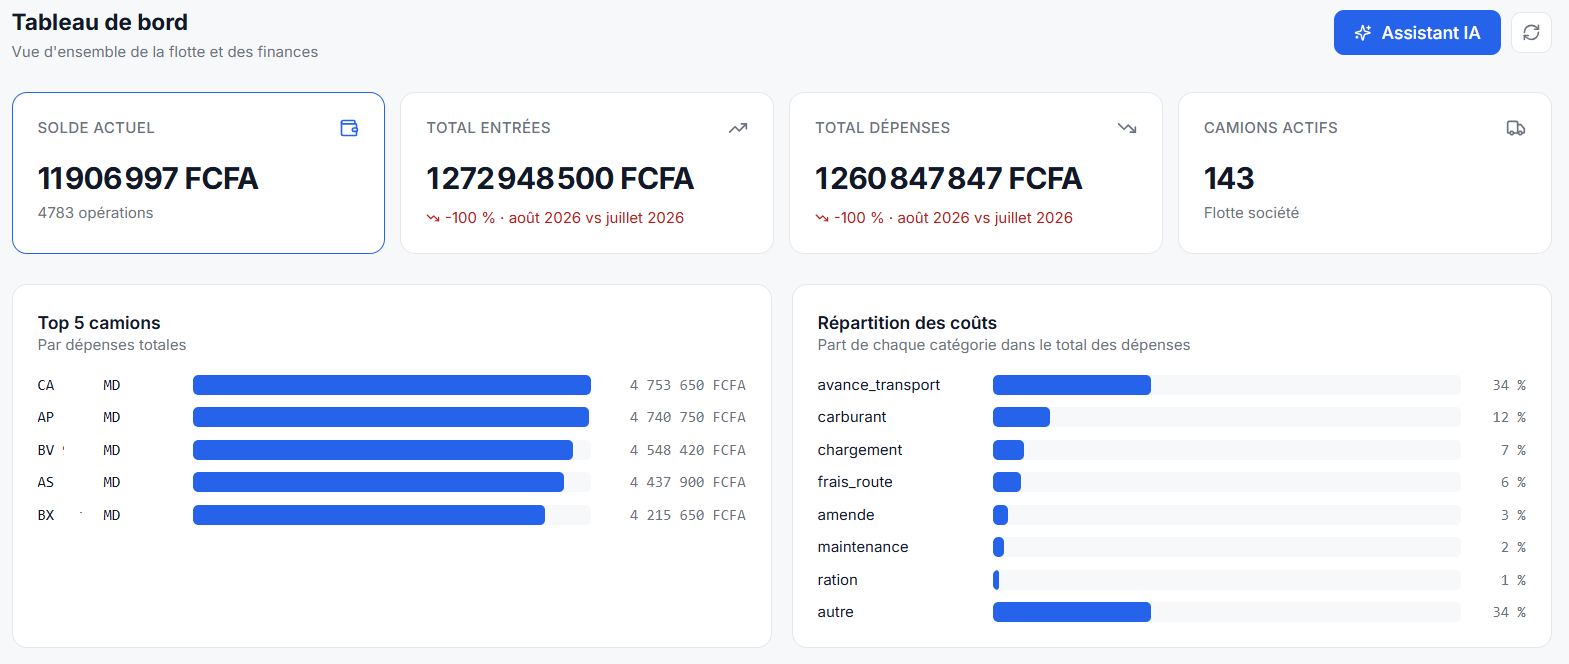
\includegraphics[width=0.85\textwidth]{figures/captures/web_dashboard.png}
    \caption{Tableau de bord : solde, entrées, dépenses, flotte active et répartition des coûts}
    \label{fig:ui_dashboard}
\end{figure}

La vue \textit{Camions} (Figure~\ref{fig:web_flotte}) réalise \texttt{EF-DSH-02} et \texttt{EF-DSH-04} : chaque carte donne l'immatriculation, le pays, la position, le total des dépenses et le nombre d'opérations, et ouvre le profil du camion.

\begin{figure}[H]
    \centering
    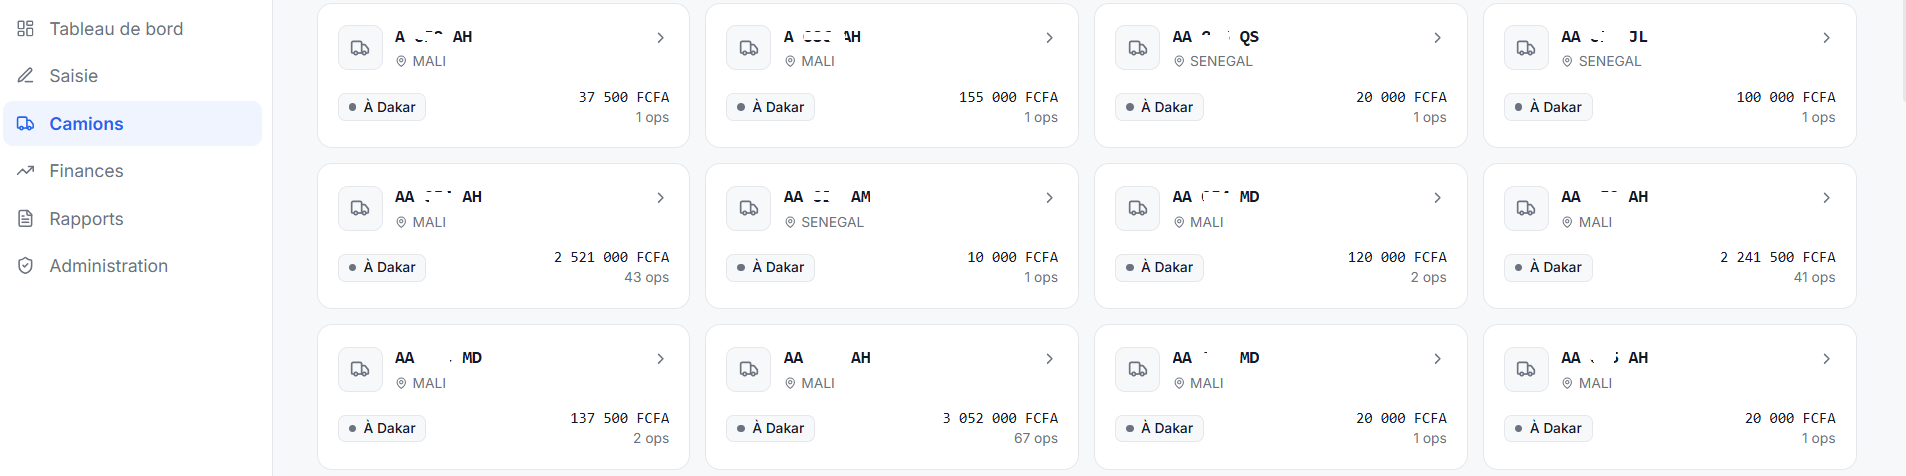
\includegraphics[width=0.85\textwidth]{figures/captures/web_flotte.png}
    \caption{Vue de la flotte par camion}
    \label{fig:web_flotte}
\end{figure}

La saisie directe (Figure~\ref{fig:web_saisie}) remplace le fichier \og RECAP-JOURNALIER \fg{} envoyé par WhatsApp. L'agent choisit le sens de l'opération, puis renseigne le libellé, la date, la catégorie, le montant et, si besoin, le camion et le bon de livraison. L'opération est visible à Bamako dès son enregistrement.

\begin{figure}[H]
    \centering
    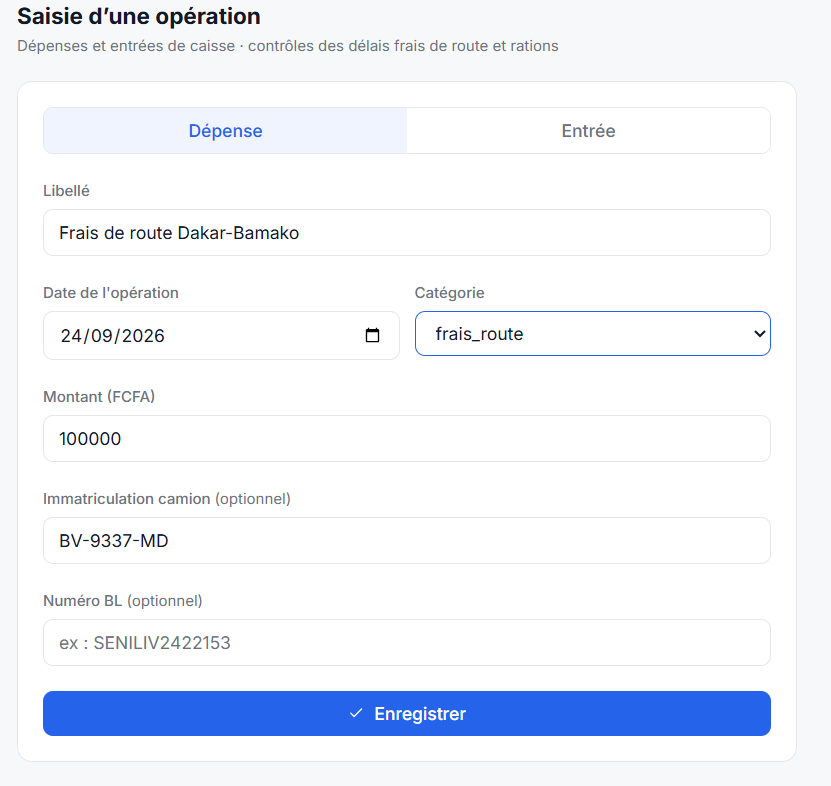
\includegraphics[width=0.5\textwidth]{figures/captures/web_saisie.png}
    \caption{Formulaire de saisie d'une opération de caisse}
    \label{fig:web_saisie}
\end{figure}

\subsection{Authentification et gestion de session}
\label{sec:webapp_jwt}

L'authentification (\texttt{ENF-SEC-01}) repose sur deux jetons. Le jeton d'accès est un JWT signé, valable huit heures ; le serveur refuse de démarrer si sa clé de signature fait moins de 64 caractères. Le jeton de rafraîchissement, valable sept jours, est une chaîne aléatoire dont seule l'empreinte SHA-256 est conservée en base : une fuite de la base ne permet donc de rejouer aucune session. Les mots de passe sont hachés par \texttt{bcrypt} (\texttt{ENF-SEC-02}).

Deux protections dépassent le cahier des charges. Un compte est verrouillé quinze minutes après cinq échecs consécutifs (Figure~\ref{fig:ui_verrouillage}). Et une adresse inconnue déclenche quand même une comparaison \texttt{bcrypt} factice : le temps de réponse ne révèle pas si un compte existe.

\begin{figure}[H]
    \centering
    \begin{minipage}{0.42\textwidth}
        \centering
        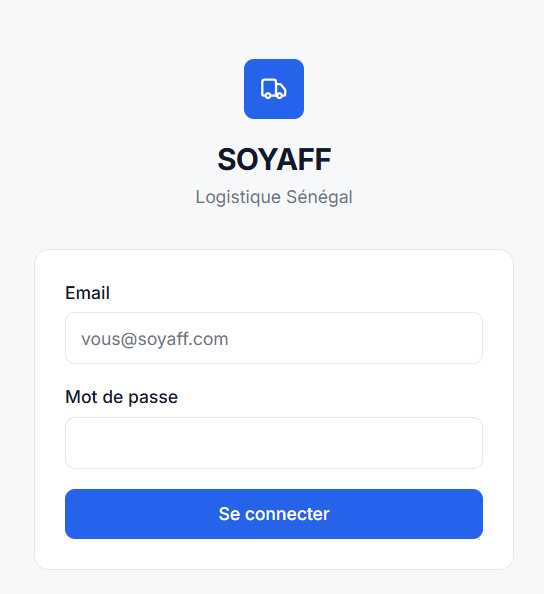
\includegraphics[width=\textwidth]{figures/captures/web_connexion.png}
        \caption{Page de connexion}
        \label{fig:web_connexion}
    \end{minipage}\hfill
    \begin{minipage}{0.48\textwidth}
        \centering
        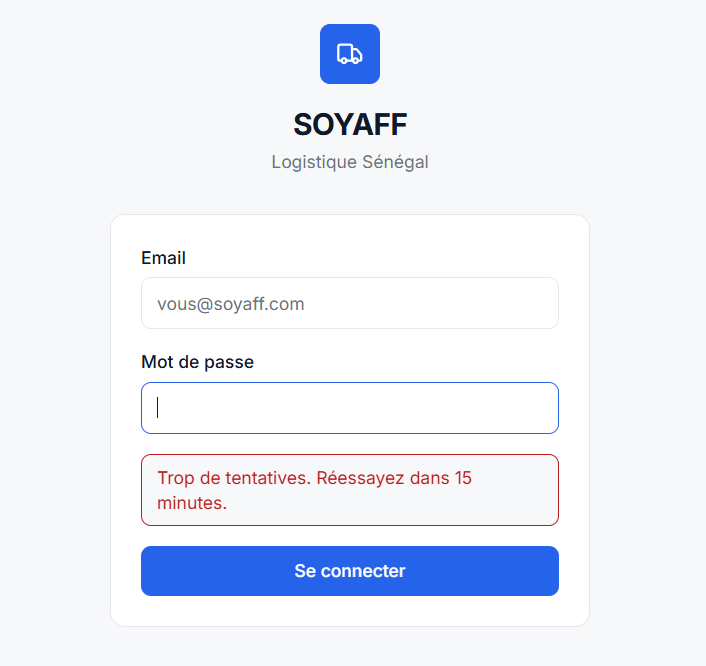
\includegraphics[width=\textwidth]{figures/captures/web_verrouillage.png}
        \caption{Compte verrouillé après cinq échecs}
        \label{fig:ui_verrouillage}
    \end{minipage}
\end{figure}

Deux arbitrages sont assumés. Les jetons sont stockés en \texttt{localStorage}, exposés à un script injecté ; la migration vers des cookies \texttt{httpOnly} est planifiée. Le jeton de rafraîchissement n'est pas renouvelé à chaque usage : il reste valable sept jours, mais la déconnexion le révoque immédiatement.

\subsection{Intégrité des données : le calcul du solde}
\label{sec:webapp_integrity}

Le diagnostic du chapitre~\ref{chap:contexte} relevait des formules de solde qui se cassaient dans les tableurs au fil des copier-coller. Le solde progressif n'est désormais calculé qu'à un seul endroit : la route de saisie \texttt{POST /api/finances/operation}, dans une transaction SQL unique. Elle garantit l'existence du camion et du bon de livraison, relit le dernier solde connu à la date de l'opération, calcule le nouveau solde et l'enregistre avec l'opération. Toute erreur annule l'ensemble : aucune opération ne peut exister sans son solde. Le frontend affiche ce solde sans jamais le recalculer. C'est le même principe que l'idempotence de l'ETL (\S\ref{sec: chargement}) : contraindre la base plutôt que discipliner l'utilisateur.

\subsection{Contrôle des délais de saisie}
\label{sec:webapp_delais}

\texttt{EF-SDR-02} demandait de contrôler l'intervalle entre deux rations d'un même chauffeur. Nous avons étendu ce contrôle aux frais de route, à la suite d'un ordre de travail du 24~septembre~2026. Les règles sont regroupées dans \texttt{utils/delais.js}, couvert par des tests :
\begin{itemize}
    \item \textbf{frais de route} : deux opérations pour un même camion doivent être espacées d'au moins 8~jours, sinon la saisie est bloquée ;
    \item \textbf{rations} : sous 2~jours, la saisie est bloquée ; entre 2 et 5~jours, l'opérateur doit confirmer une alerte.
\end{itemize}
Le chauffeur est rattaché à son camion dans la table \texttt{chauffeurs}. L'écart est mesuré par rapport à l'opération la plus proche, avant \emph{ou} après : une saisie antidatée est contrôlée comme les autres. Le contrôle s'exécute dans l'API, pas seulement dans le formulaire. Seul un administrateur peut lever un blocage ; forçage et confirmation sont inscrits dans \texttt{audit\_logs}. Les Figures~\ref{fig:web_delai_agent} et~\ref{fig:web_delai_admin} montrent la même saisie vue par un agent puis par un administrateur.

\begin{figure}[H]
    \centering
    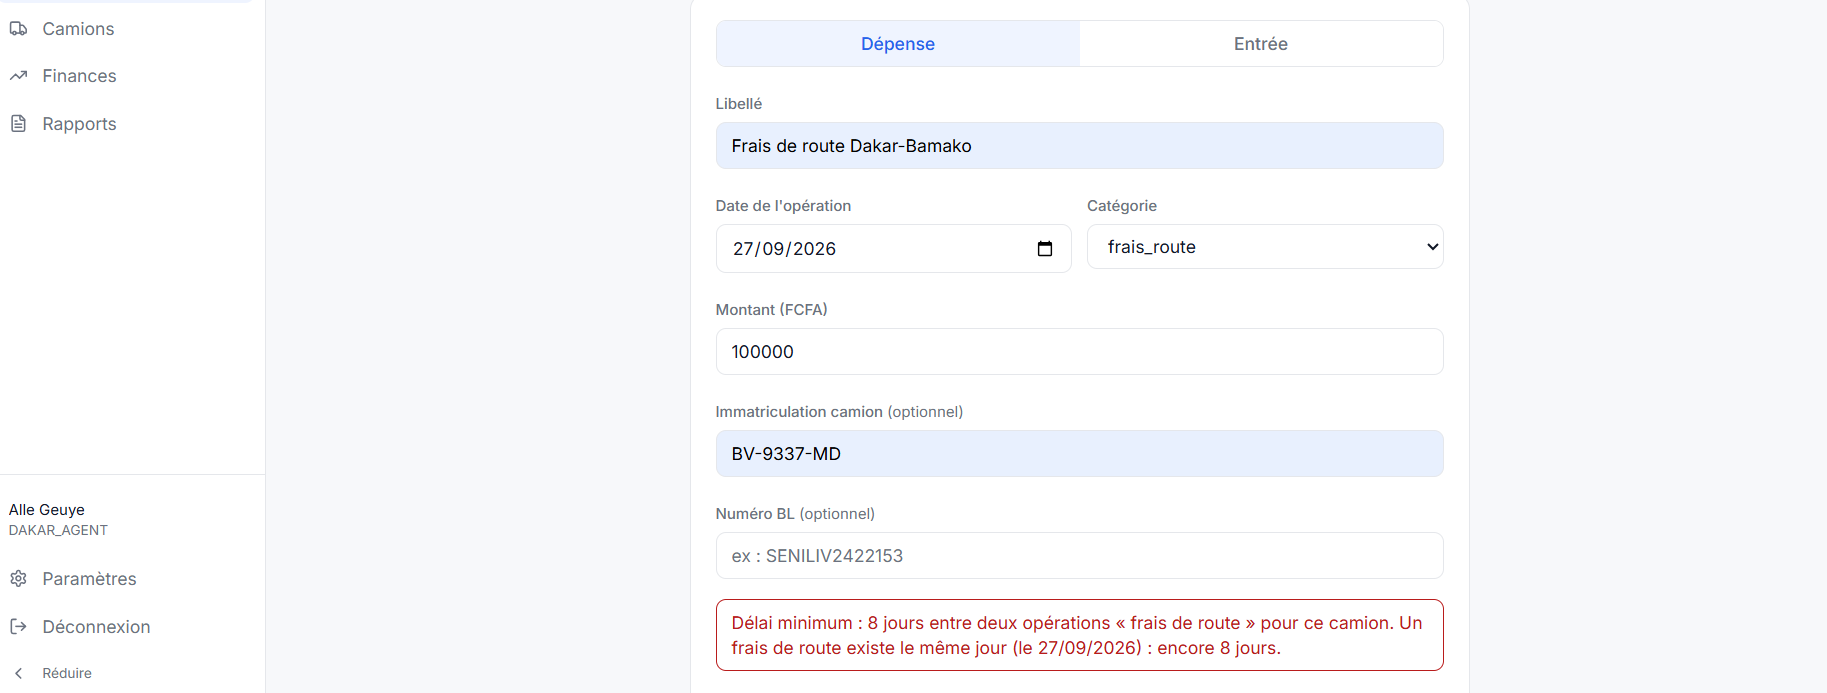
\includegraphics[width=0.8\textwidth]{figures/captures/web_delai_agent.png}
    \caption{Frais de route saisi deux fois le même jour, profil agent de Dakar : saisie bloquée}
    \label{fig:web_delai_agent}
\end{figure}

\begin{figure}[H]
    \centering
    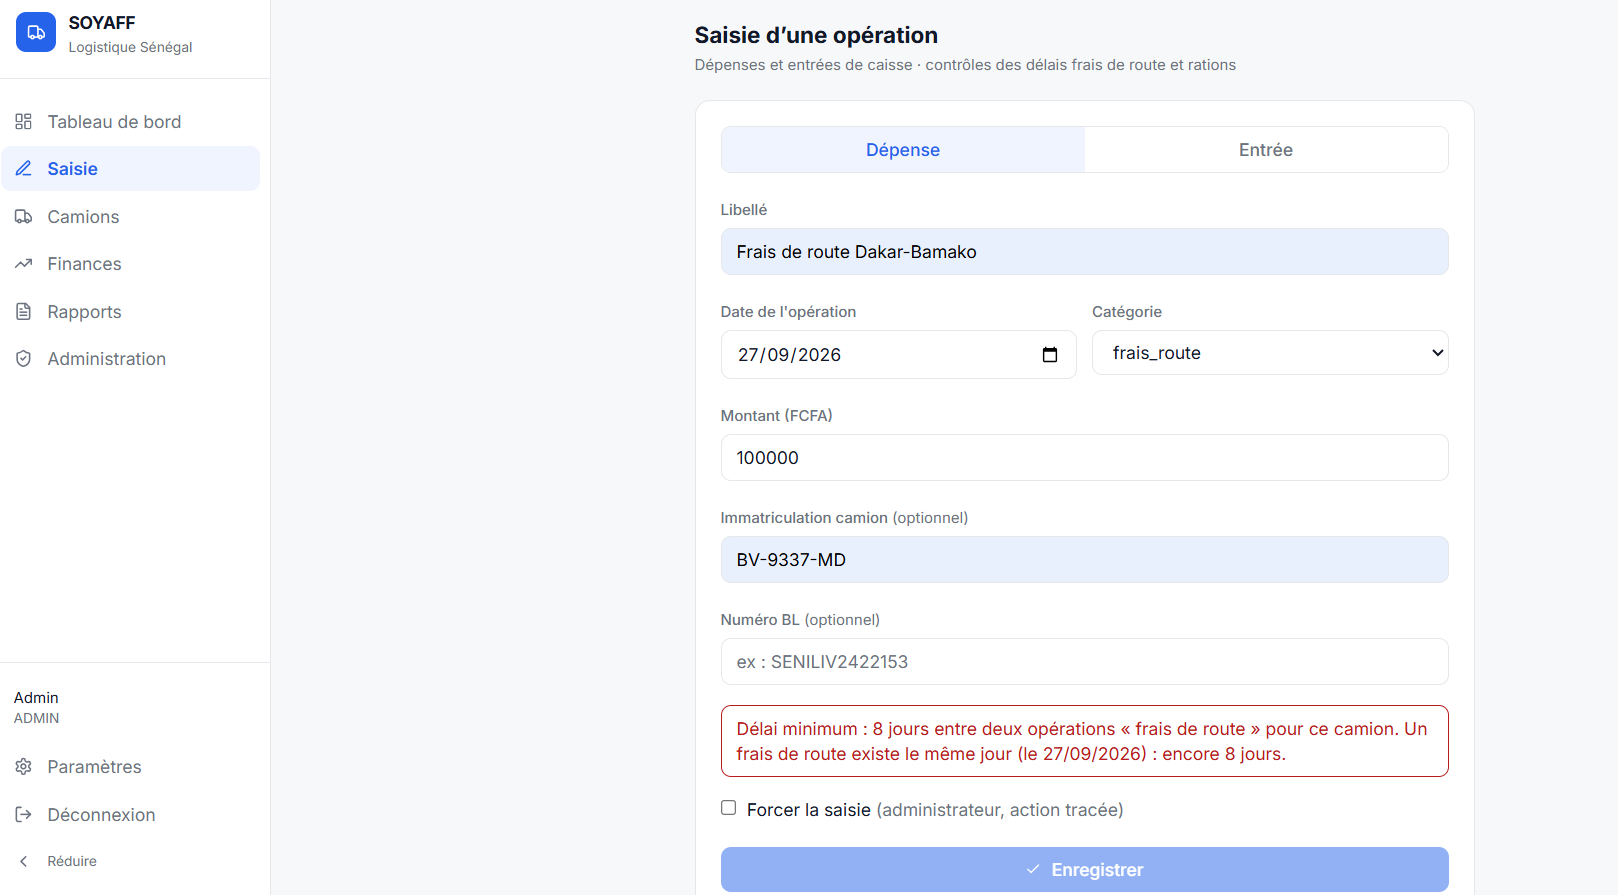
\includegraphics[width=0.7\textwidth]{figures/captures/web_delai_admin.png}
    \caption{Même saisie, profil administrateur : forçage possible et tracé}
    \label{fig:web_delai_admin}
\end{figure}

\subsection{Contrôle d'accès (RBAC) et audit}
\label{sec:webapp_rbac}

Trois rôles (\texttt{DAKAR\_AGENT}, \texttt{BAMAKO\_CHEF}, \texttt{ADMIN}) reprennent les personas de la section~\ref{chap:besoins} (\S\ref{sec:personas}). La liste est contrainte à trois niveaux : l'interface ne propose que ces valeurs, l'API rejette toute autre valeur, et une contrainte \texttt{CHECK} sur la colonne \texttt{users.role} protège la base contre toute écriture qui contournerait l'API (\texttt{ENF-SEC-03}).

Le middleware \texttt{authorize()} vérifie le rôle sur chaque route protégée. En cas de refus, il inscrit lui-même la tentative dans \texttt{audit\_logs} (\texttt{UNAUTHORIZED\_ACCESS}) avant de répondre \texttt{403}. La même table reçoit les actions d'administration réussies : création de compte, changement de rôle, réinitialisation de mot de passe (\texttt{EF-ADM-02}). Elle couvre ainsi les deux volets de \texttt{ENF-SEC-04}, résumés par la Figure~\ref{fig:seq_rbac_audit}. Un administrateur ne peut pas désactiver son propre compte ; désactiver un compte révoque ses sessions ; aucun compte n'est supprimé, pour préserver l'historique d'audit.

\begin{figure}[H]
    \centering
    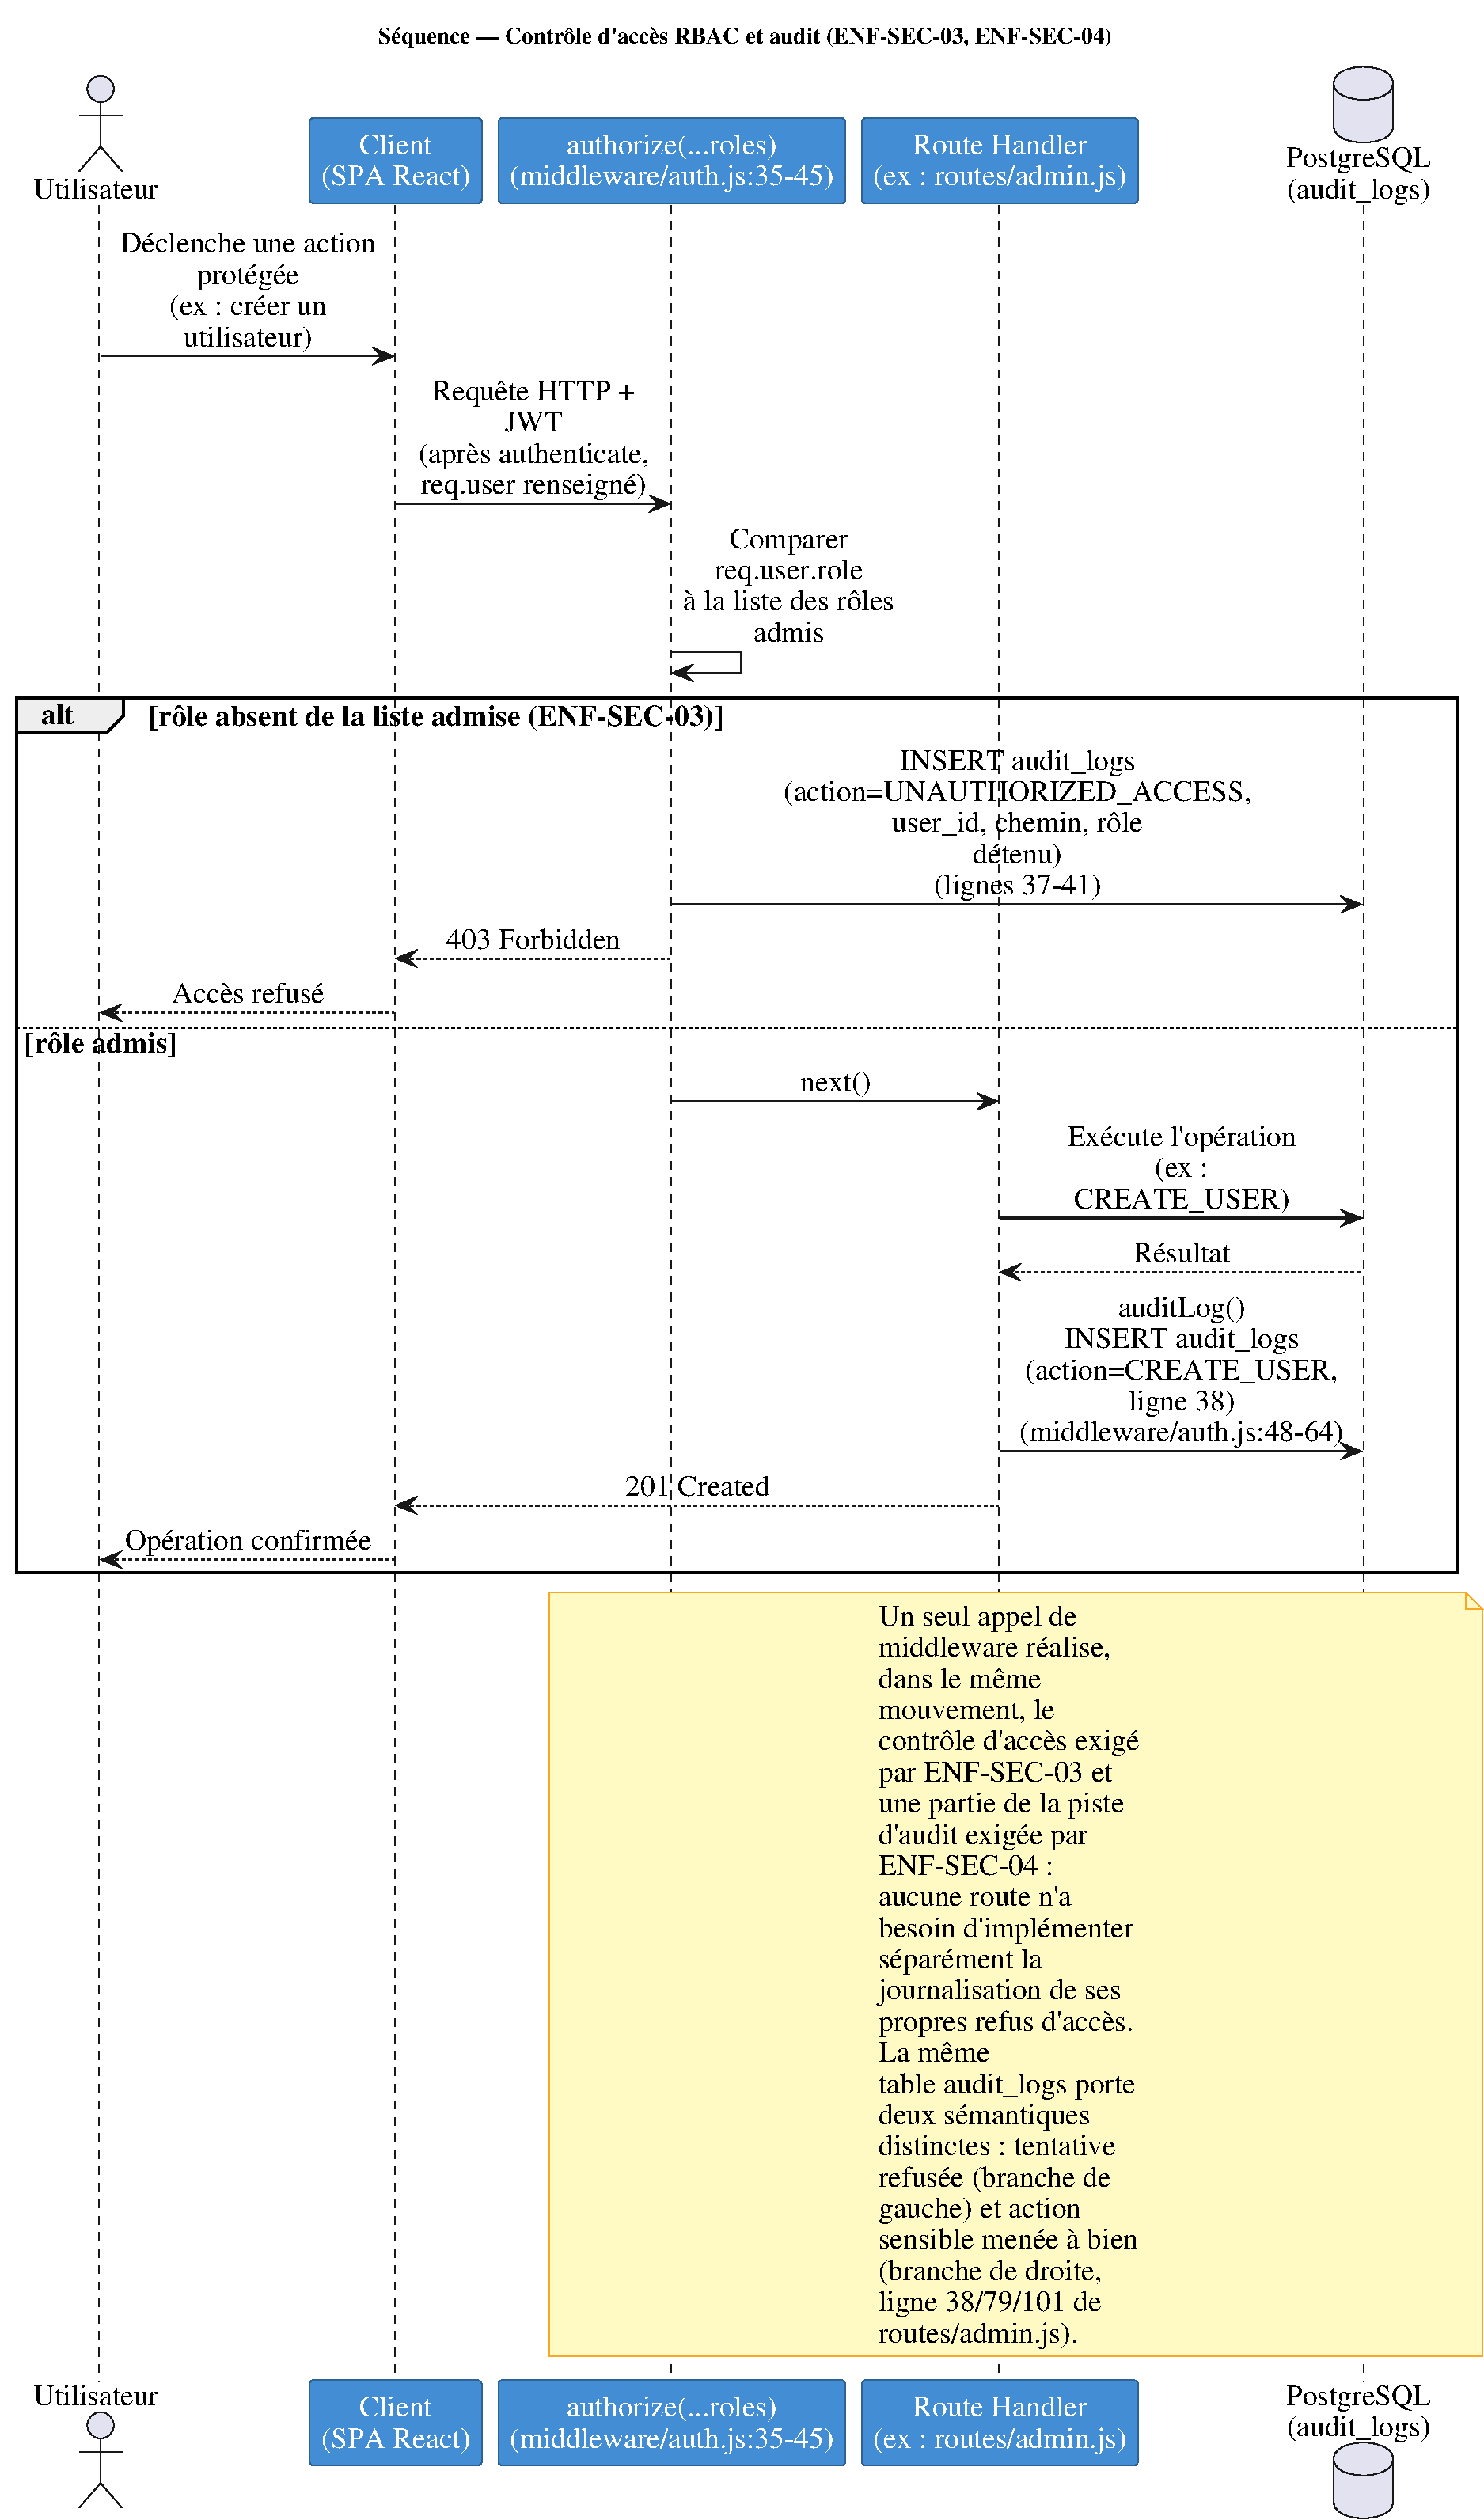
\includegraphics[width=\textwidth,height=0.88\textheight,keepaspectratio]{figures/fig_seq_rbac_audit.pdf}
    \caption{Séquence : contrôle d'accès RBAC et audit}
    \label{fig:seq_rbac_audit}
    \source{Schéma de l'auteur}
\end{figure}

\subsection{Reporting et export}
\label{sec:webapp_reporting}

Les récapitulatifs journalier et mensuel (\texttt{EF-REP-01}, \texttt{EF-REP-02}) et la recherche par période, camion ou catégorie (\texttt{EF-REP-04}) sont déployés. La Figure~\ref{fig:web_rapport} montre le rapport de juillet~2026 : totaux, solde de fin de mois, répartition des dépenses, classement des camions et détail chronologique.

\begin{figure}[H]
    \centering
    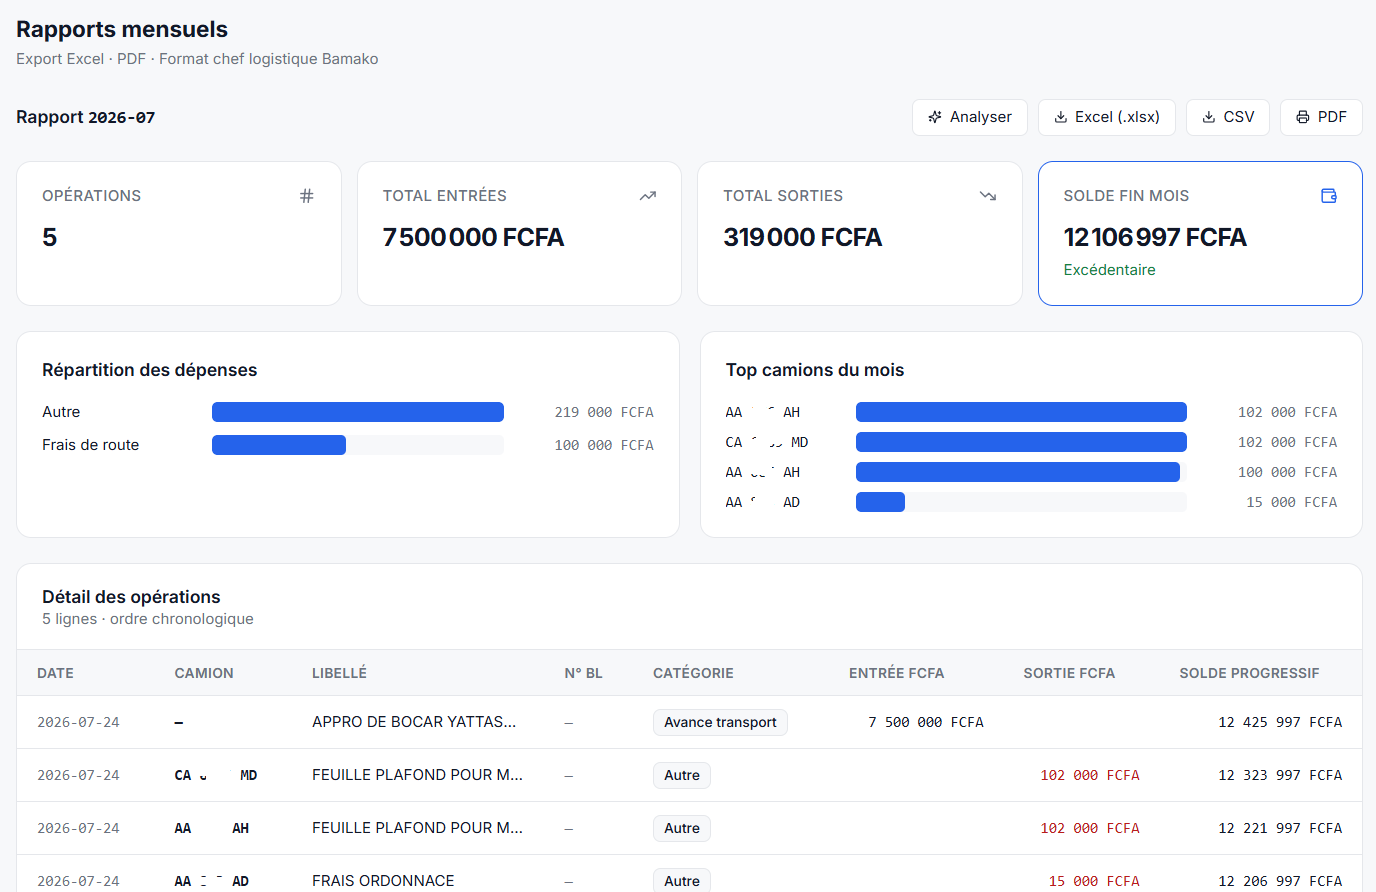
\includegraphics[width=0.75\textwidth]{figures/captures/web_rapport.png}
    \caption{Rapport mensuel consolidé (juillet~2026)}
    \label{fig:web_rapport}
\end{figure}

L'export (\texttt{EF-REP-03}) est partiel. Le CSV respecte l'usage français (encodage UTF-8 avec BOM, séparateur point-virgule) et s'ouvre directement dans Excel. Le fichier Excel est construit par le serveur, avec une feuille de résumé et une feuille de détail (Figure~\ref{fig:web_export}). Le bouton « PDF », en revanche, lance seulement l'impression du navigateur : aucun PDF n'est produit par le serveur. Un vrai export PDF est renvoyé aux perspectives.

\begin{figure}[H]
    \centering
    
\includegraphics[width=0.8\textwidth]{figures/captures/web_export_xlsx.png}
    \caption{Export Excel du rapport mensuel : fichier \texttt{rapport-2026-07.xlsx} généré par le serveur}
    \label{fig:web_export}
\end{figure}

\subsection{Fonctionnalités cibles non déployées}
\label{sec:webapp_fonctionnalites_cibles_non_deployees}

\textbf{EF-VAL-02 : workflow de validation.} Chaque opération est enregistrée directement et définitivement : il n'existe ni statut (brouillon, validé), ni circuit d'approbation. Le visa manuscrit reste la référence pendant la transition, choix de priorité déjà justifié à la section~\ref{chap:besoins} (\S\ref{sec:synthese_tracabilite}) et représenté par le diagramme d'activité cible (Figure~\ref{fig:activite_validation_cible}).

\textbf{ENF-DISP-01 : mode hors-ligne.} Aucun mécanisme de saisie hors connexion n'existe : c'est une cible non entamée.

Ces deux manques ne remettent en cause ni la fin de la double saisie ni la visibilité en temps réel, déjà obtenues. Leur priorisation est discutée à la section~\ref{chap:discussion}.

\subsection{Synthèse et transition}
\label{sec:webapp_synthese_transition}

L'application réalise le cœur du cahier des charges : saisie unique et contrôlée, solde calculé par la base, accès cloisonné par rôle avec piste d'audit, rapports et exports. Elle reste une exploitation structurée, par formulaires et filtres. L'interrogation des données en langage naturel fait l'objet de la section suivante.

\section{Module d'IA générative hybride (RAG local et agent cloud)}
\label{chap:ia_rag}

Cette section décrit le module qui porte la contribution la plus distinctive de la plateforme : un agent conversationnel hybride, au sens défini en introduction. Un service local auto-hébergé (Mistral~7B via Ollama) traite les requêtes sensibles, qui doivent rester sous le contrôle de l'entreprise. Un service cloud (\texttt{claude-sonnet-4-5}, API Anthropic) traite les requêtes analytiques non sensibles, qui demandent une plus grande capacité de raisonnement. Nous décrivons ici la construction des deux chemins et du mécanisme qui les arbitre ; leur évaluation comparative, qui porte l'hypothèse H2, fait l'objet de la section~\ref{chap:benchmark_rag}.

\subsection{Architecture d'ensemble du module conversationnel hybride}
\label{sec:ia_archi}

Une requête suit toujours le même trajet. L'utilisateur la saisit dans le panneau conversationnel, ouvert par le bouton \textit{Assistant IA} de l'application (Figure~\ref{fig:ui_dashboard}). Un proxy de l'API Express la relaie à l'orchestrateur n8n, qui en évalue la sensibilité et la route vers l'un des deux chemins. L'échange est ensuite journalisé, quel que soit le chemin emprunté. Ce trajet est celui de la Figure~\ref{fig:seq_rag} (séquence) et de la Figure~\ref{fig:c4_conteneurs} (conteneurs) ; cette section en détaille l'implémentation.

\textbf{n8n comme point d'orchestration unique.} C'est le workflow n8n, et non l'application Express ou le service FastAPI, qui porte la logique hybride : il reçoit chaque requête, en évalue la sensibilité et décide du chemin (\texttt{EF-RAG-03}, ADR-02, \S\ref{sec:adr}). Les deux chemins augmentent la génération par des données métier réelles, mais par des mécanismes de récupération différents. Côté cloud (\S\ref{sec:ia_cloud}), un agent génère lui-même une requête SQL sur les vues relationnelles de la base. Côté local (\S\ref{sec:ia_local}), c'est le code du service qui récupère les données : par des filtres SQL déterministes (plaque, période, mots-clés) d'abord, par similarité vectorielle sur le corpus produit par l'ETL (\S\ref{sec:  vectorisation}) en dernier recours. Les deux relèvent du paradigme RAG au sens large : récupérer un contexte pertinent avant de générer.

\textbf{Le proxy Express.} Les routes qui relaient la requête vers n8n vivent dans le dépôt applicatif (section~\ref{chap:webapp}), mais relèvent de ce module. \texttt{POST~/api/chat} (\texttt{routes/chat.js}) est la route utilisée par le panneau conversationnel. Elle valide le message, le relaie au \textit{webhook} n8n avec un délai d'attente dimensionné pour les itérations d'un agent outillé, normalise la réponse et journalise l'échange dans \texttt{chat\_messages} (\S\ref{sec:ia_tracabilite}). Elle transmet aussi au client le chemin emprunté (\texttt{local} ou \texttt{cloud}), que l'interface affiche sous chaque réponse. \texttt{GET~/api/chat/history} expose l'historique d'un utilisateur. La route \texttt{POST~/api/analyze} (\texttt{index.js}) relaie elle aussi vers n8n, mais aucun composant du frontend ne l'appelle : c'est du code mort, que nous signalons comme tel.

\subsection{Le service RAG local souverain}
\label{sec:ia_local}

Le service FastAPI du chemin local est celui qui incarne le plus directement la souveraineté visée par H2 : un RAG conversationnel sur un corpus métier français, sans dépendance à un service tiers. Nous l'avons construit selon le schéma \textit{retriever--augmentation--generator} de Lewis et al. \cite{lewisRetrievalaugmentedGenerationKnowledgeintensive2020} (\S\ref{sec:Systemes_RAG_IA_Generative}), adapté à un corpus structuré et très redondant.

\subsubsection{Le retrieval : SQL exact d'abord, vectoriel en dernier recours}

\texttt{fetch\_rows()} applique une stratégie par passes successives. Elle repose sur une hypothèse simple : une correspondance exacte sur un identifiant métier (une plaque, une période, un mot du domaine) est un signal plus fiable qu'une similarité sémantique.

\begin{itemize}
    \item \textbf{Passe~0, la plaque.} Une immatriculation détectée dans la question filtre la vue \texttt{v\_transactions\_completes} sur la colonne \texttt{camion}, éventuellement croisée avec la période. Elle est prioritaire et isolée des autres mots-clés, pour ne pas diluer ce signal fort (« CAMION » figure dans des centaines de libellés sans rapport avec le véhicule visé).
    \item \textbf{Passes~1 et~2, les mots-clés.} Vingt et un mots déclencheurs du domaine (\textit{ex.} \texttt{CARBURANT}, \texttt{VIDANGE}, \texttt{RATION}) sont cherchés dans les libellés, d'abord en conjonction stricte, puis en disjonction. Certains sont traduits vers le vocabulaire réel de la base : « amende » ne figure dans aucun libellé, ce sont « contravention », « pesage » ou « défaut de papier » qui y figurent.
    \item \textbf{Filtres transverses.} Une période exprimée en toutes lettres (« mars 2026 », « T1 2026 ») ou au format ISO, et des critères de flotte (pays, type de propriété, statut) s'ajoutent en conjonction à toutes les passes. Si une question filtrée ne trouve rien, le service répond « aucune donnée » plutôt que de se replier sur une recherche vectorielle qui ignorerait le filtre.
    \item \textbf{Passe~3, le repli vectoriel.} Seulement si tout le reste échoue : la question est encodée par le même modèle qu'à l'ingestion (\texttt{all-MiniLM-L6-v2} \cite{reimersSentencebertSentenceEmbeddings2019}), puis comparée à \texttt{transport\_embeddings} par similarité cosinus (opérateur \texttt{<=>} de \texttt{pgvector}), qui renvoie les $k=10$ passages les plus proches \cite{karpukhinDensePassageRetrieval2020}.
\end{itemize}

\begin{lstlisting}[language=SQL, basicstyle=\ttfamily\footnotesize, breaklines=true, showstringspaces=false]
SELECT date, libelle, sortie FROM transport_embeddings
ORDER BY embedding <=> %s::vector ASC LIMIT 10
\end{lstlisting}

\textbf{Des réponses exactes sans modèle de langage.} Les LLM sont peu fiables en arithmétique. Nous avons donc retiré au modèle tout calcul qu'une requête SQL peut faire. Pour les passes~0 à~2, le total et le nombre d'opérations sont calculés par \texttt{SUM} et \texttt{COUNT} sur \emph{toutes} les lignes qui correspondent au filtre, pas seulement sur les dix transmises au modèle. Trois familles de questions sont ensuite servies directement, sans appel au LLM :
\begin{itemize}
    \item les comptages de camions (« combien de camions maliens actifs ? »), par un \texttt{COUNT} SQL ;
    \item le solde de caisse, calculé selon la même définition que la carte « Solde actuel » du tableau de bord ;
    \item les demandes d'agrégat (« total », « somme », « combien »), qui reçoivent le total SQL déjà calculé.
\end{itemize}
Pour les autres questions, le total est placé en tête du contexte, avec la mention « TOTAL EXACT (déjà calculé, à recopier tel quel) ». Pour le repli vectoriel, qui n'a pas de filtre exploitable, la mention devient « TOTAL APPROXIMATIF ». La part des questions du benchmark servies sans LLM est mesurée à la section~\ref{chap:benchmark_rag}.

\subsubsection{La génération}

Les questions ouvertes sont transmises à Mistral~7B par l'API de conversation d'Ollama (\texttt{http://ollama:11434/api/chat}), sous forme d'un message système et d'un message utilisateur contenant le contexte. Le message système impose une réponse en français de trois ou quatre phrases, la recopie mot pour mot du total fourni, la citation de deux ou trois postes de dépense représentatifs et l'aveu explicite d'une information absente. Nous avons fixé la température à~0,1, pour des réponses stables d'un appel à l'autre, et limité la sortie à 300~jetons. Le nom du modèle (\texttt{mistral:latest}) est écrit en dur dans la requête, et le message système est dupliqué entre les deux fonctions de génération : deux dettes de maintenabilité (\texttt{ENF-MAINT-01}, \texttt{ENF-MAINT-02}) reprises au §\ref{sec:ia_dettes}.

\subsubsection{Les points d'entrée}

Le service expose deux \textit{endpoints}, authentifiés par l'en-tête \texttt{X-API-Key} : \texttt{POST~/ask} renvoie la réponse complète en un bloc JSON ; \texttt{POST~/ask/stream} la restitue jeton par jeton. Le streaming répond à une contrainte d'usage : sans accélération matérielle (ADR-03, \S\ref{sec:adr}), l'inférence est lente, et une réponse qui se construit progressivement vaut mieux qu'un long silence. Un \textit{endpoint} \texttt{/health}, public et sans donnée, sert au contrôle de santé du conteneur (Figure~\ref{fig:ia_rag_api_logs}).

\begin{figure}[H]
    \centering
    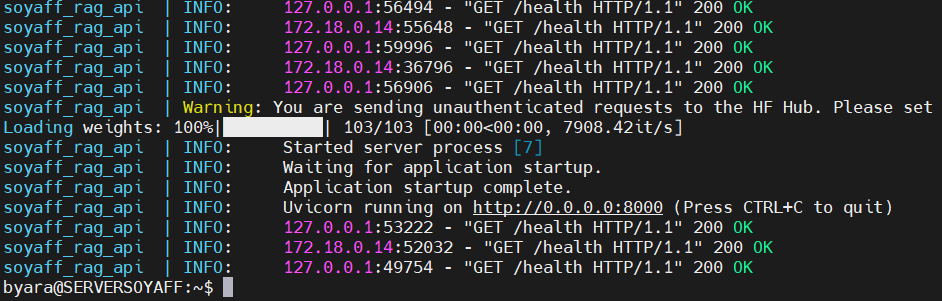
\includegraphics[width=0.65\textwidth]{figures/captures/ia_rag_api_logs.png}
    \caption{Démarrage du service RAG local en production et sondes de santé périodiques}
    \label{fig:ia_rag_api_logs}
\end{figure}

\textbf{Souveraineté par construction.} Sur ce chemin, aucune donnée de la base ne sort du serveur : le \textit{retrieval} interroge PostgreSQL en local, l'inférence s'exécute dans le conteneur Ollama du même réseau Docker, et seule la réponse finale est renvoyée à n8n. Cette étanchéité réalise \texttt{ENF-SOUV-01} pour ce chemin ; c'est un fait de construction, pas encore une mesure.

\subsection{Le chemin cloud}
\label{sec:ia_cloud}

Le second chemin traite les requêtes analytiques non sensibles (\texttt{EF-RAG-01}, \texttt{EF-RAG-02}) : agrégations, comparaisons temporelles, classements sur l'ensemble du référentiel. Pour ces requêtes, la capacité de raisonnement d'un grand modèle l'emporte sur la contrainte de souveraineté (\S\ref{sec:Systemes_RAG_IA_Generative}).

\textbf{Le modèle et son emplacement.} Le modèle est \texttt{claude-sonnet-4-5-}\allowbreak\texttt{20250929} de l'API Anthropic. L'appel n'est fait nulle part dans le code Express : il est porté par un nœud \textit{AI Agent} de n8n (\textit{framework} LangChain), connecté à un nœud de modèle Anthropic. Le proxy applicatif ignore l'existence de ce modèle.

\begin{sloppypar}
\textbf{Un agent outillé.} L'agent dispose d'un outil d'exécution SQL sur PostgreSQL. La requête est générée par le modèle à partir d'un \textit{system prompt} versionné (\texttt{n8n/system\_prompt\_agent.md}), qui documente les vues métier (\texttt{v\_transactions\_completes}, \texttt{v\_stats\_par\_camion}, \texttt{v\_resume\_mensuel}, \texttt{v\_stats\_par\_produit}), les conventions du domaine et des exemples de correspondance question--requête. Une mémoire conversationnelle, également dans PostgreSQL, conserve les dix derniers échanges d'une session : l'agent peut ainsi résoudre « ce camion » dans une question de relance. La réponse suit un gabarit imposé : tableau, analyse, recommandation le cas échéant.
\end{sloppypar}

\textbf{Un accès en lecture seule.} Le SQL généré par un modèle ne doit pas pouvoir modifier la base. Nous avons donc connecté l'outil SQL à un rôle PostgreSQL dédié, \texttt{soyaff\_agent\_ro} (migration Alembic~004). Ses sessions sont en lecture seule par défaut, ses requêtes sont interrompues au-delà de 15~secondes et il ne peut ouvrir que cinq connexions. Il ne lit que les tables et vues métier ; la table \texttt{chauffeurs} (noms, téléphones), les embeddings et l'historique des conversations lui sont inaccessibles. La mémoire de conversation utilise un autre compte. La garantie ne repose donc plus sur l'obéissance du modèle aux consignes, mais sur les droits de la base (voir le test du §\ref{sec:test_bout_en_bout}).

\textbf{Une frontière franchie.} Ce chemin traverse le périmètre souverain de la Figure~\ref{fig:c4_conteneurs} : la question de l'utilisateur et les résultats des requêtes SQL de l'agent sont traités par un service tiers. Le routage décrit ci-dessous existe pour limiter ce franchissement aux requêtes non sensibles.

\subsection{Le routage par sensibilité}
\label{sec:ia_routage}

Le routage est le mécanisme qui fait exister l'hybride au sens de l'introduction ; il réalise \texttt{EF-RAG-03}. Chaque requête entre dans le workflow n8n de la Figure~\ref{fig:ia_workflow}, dont le premier nœud de code en évalue la sensibilité. Une requête sensible part vers le service local par une requête HTTP authentifiée (\texttt{POST~http://api:8000/ask}) ; une requête non sensible est confiée à l'agent cloud. Nous avons formalisé cette décision dans l'\texttt{ADR-02} (\S\ref{sec:adr}) : un point de décision unique plutôt qu'une logique dispersée dans chaque service.

\begin{figure}[H]
    \centering
    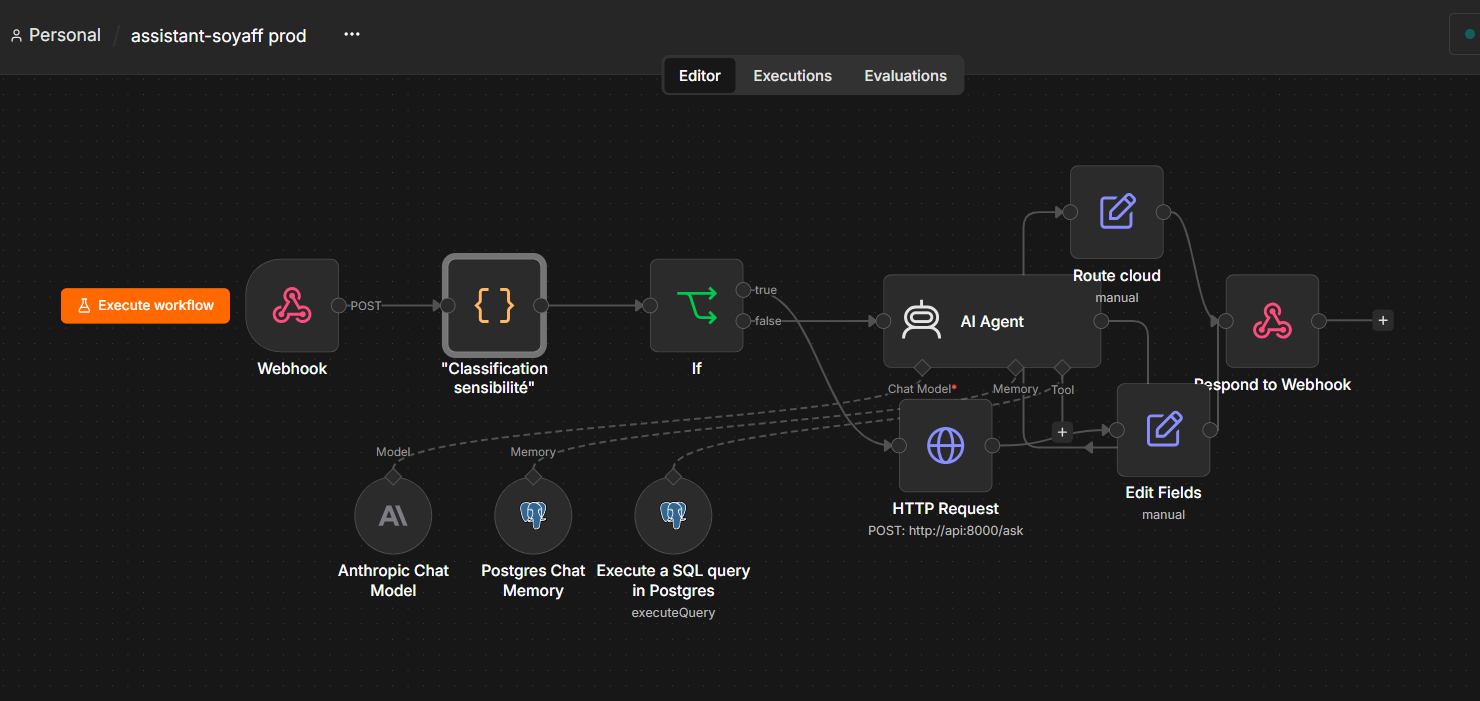
\includegraphics[width=0.85\textwidth]{figures/captures/ia_workflow_n8n.png}
    \caption{Workflow n8n de routage hybride en production}
    \label{fig:ia_workflow}
\end{figure}

\textbf{Le mécanisme.} La classification est une heuristique par mots entiers et expressions régulières, appliquée à la question débarrassée de ses accents et mise en majuscules (Figure~\ref{fig:ia_classifieur}). Ce n'est pas un classifieur d'apprentissage automatique, ainsi que l'assume l'\texttt{ADR-02}. Deux règles décident :
\begin{itemize}
    \item toute mention d'\textbf{identité} reste locale, même dans une question d'agrégat : un terme comme \textit{chauffeur}, \textit{salaire}, \textit{paie}, \textit{téléphone}, \textit{CNI} ou \textit{adresse}, ou une plaque d'immatriculation (« total du camion AA~076~AH », « top des chauffeurs ») ;
    \item un \textbf{montant financier précis} (\textit{solde}, \textit{reliquat}, \textit{avance}, « combien doit ») reste local, \emph{sauf} si la question est explicitement agrégée (\textit{total}, \textit{moyenne}, \textit{comparaison}, \textit{tendance}, \textit{top}, \textit{classement}, \textit{évolution}, pourcentage).
\end{itemize}
La seconde règle traduit un choix assumé : tout le métier de SOYAFF est financier, et classer sensible toute mention de montant viderait le chemin cloud de son utilité. La recherche par mot entier évite les faux déclencheurs (« TOP » dans « STOP », « PAIE » dans « PAIEMENT »), et le motif de plaque écarte les faux positifs du français courant (« EN 2025 », « DE 1500 »).

\begin{figure}[H]
    \centering
    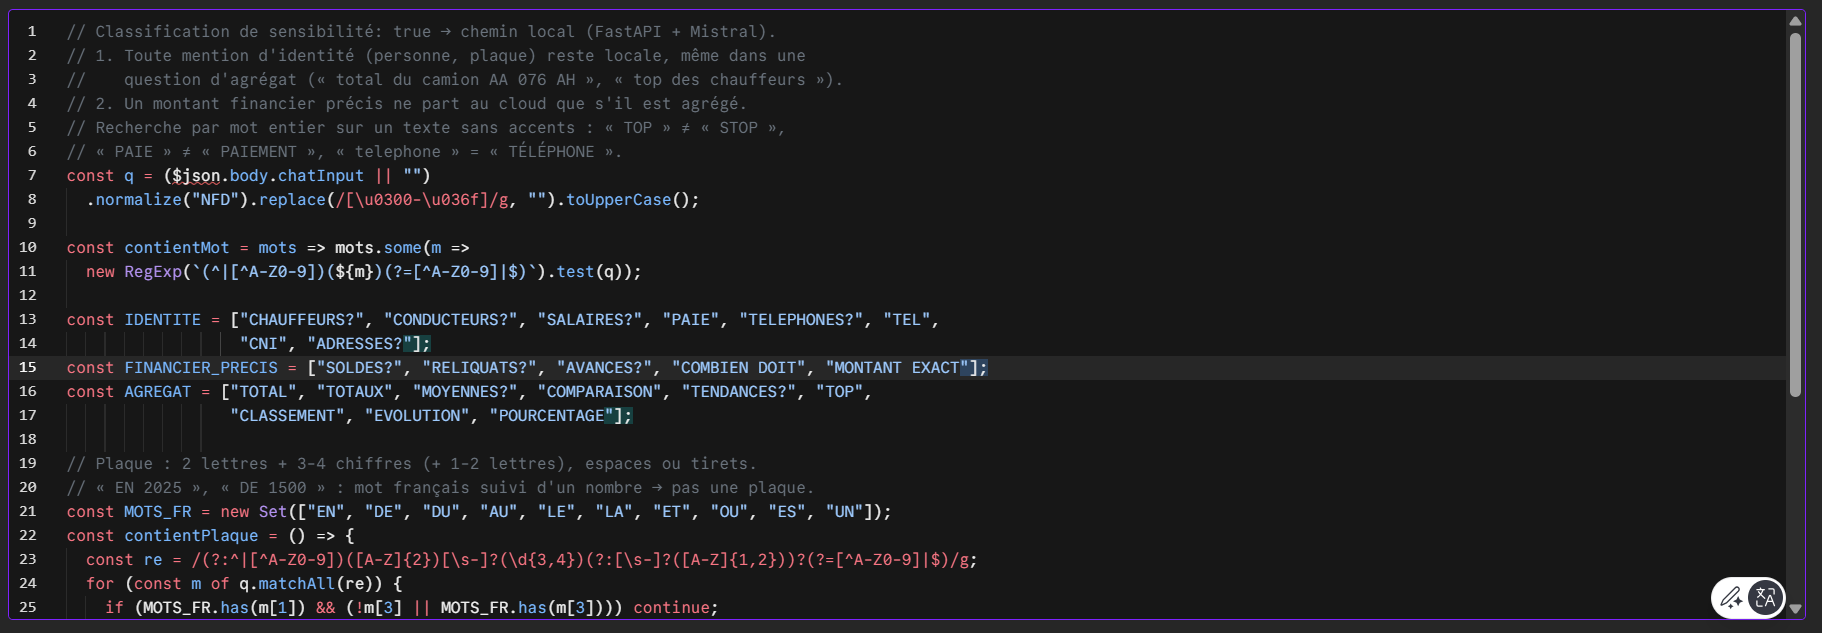
\includegraphics[width=0.9\textwidth]{figures/captures/ia_classifieur.png}
    \caption{Règles du classifieur de sensibilité (nœud de code n8n, extrait)}
    \label{fig:ia_classifieur}
\end{figure}

\textbf{Le routage vérifié.} Les Figures~\ref{fig:ia_route_locale} et~\ref{fig:ia_route_cloud} montrent les deux chemins en production. Une question sur les dépenses d'un camion identifié est traitée en local : la réponse est un total SQL exact, sans appel au LLM. Une question agrégée sur la flotte est traitée par l'agent cloud, qui répond par un tableau, une analyse et des recommandations. L'étiquette affichée sous chaque réponse indique le chemin emprunté, jamais le modèle utilisé.

\begin{figure}[H]
    \centering
    \begin{minipage}[t]{0.48\textwidth}
        \centering
        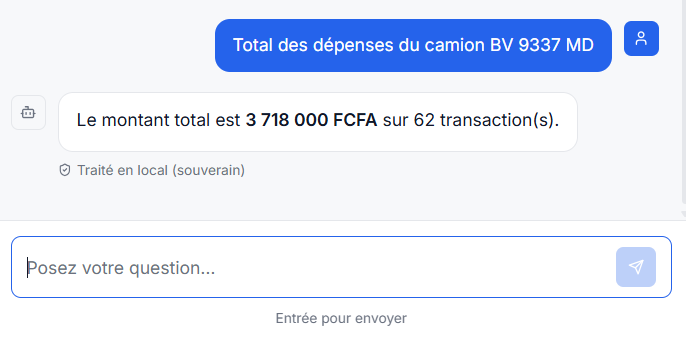
\includegraphics[width=\textwidth]{figures/captures/ia_route_locale.png}
        \caption{Question portant sur un camion identifié : traitée en local (souverain)}
        \label{fig:ia_route_locale}
    \end{minipage}\hfill
    \begin{minipage}[t]{0.48\textwidth}
        \centering
        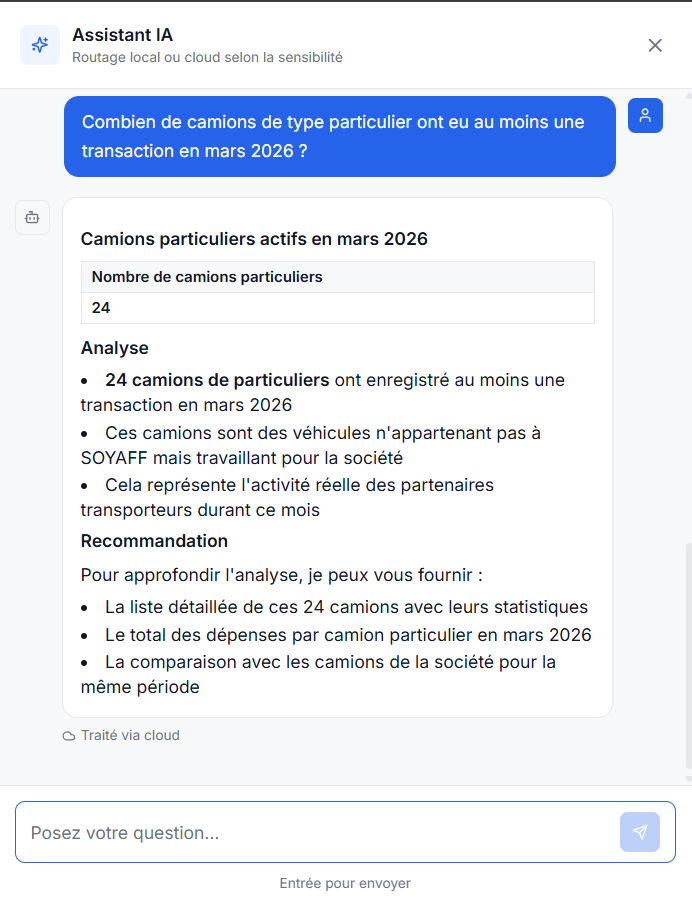
\includegraphics[width=\textwidth]{figures/captures/ia_route_cloud.png}
        \caption{Question agrégée sur la flotte : traitée via le cloud}
        \label{fig:ia_route_cloud}
    \end{minipage}
\end{figure}

\textbf{Une limite résiduelle.} L'heuristique reste lexicale. Un nom de chauffeur cité seul, sans le mot « chauffeur » ni plaque, n'est pas détecté : la requête part vers le cloud. Le risque est borné par le rôle en lecture seule (\S\ref{sec:ia_cloud}) : l'agent n'a pas accès à la table \texttt{chauffeurs} et ne peut donc pas associer ce nom à des données personnelles. Le workflow est versionné dans le dépôt \texttt{assistant-soyaff-1} (\texttt{n8n/assistant-soyaff-hybrid-routing.json}) : la classification, les deux branches et leur authentification sont reproductibles indépendamment de l'instance n8n en production.

\textbf{La conséquence méthodologique.} L'hypothèse H2 porte sur la parité d'exactitude entre les deux \emph{services d'inférence}, pas sur la justesse du classifieur qui choisit entre eux. Mesurer H2 à travers le chemin réellement emprunté par n8n ferait dépendre le résultat de la précision du classifieur, une autre question. Le benchmark de la section~\ref{chap:benchmark_rag} interroge donc chaque service directement, sur le même jeu de questions. La validité du classifieur est un chantier d'évaluation distinct, non couvert par H2.

\subsection{Citation des sources et journalisation}
\label{sec:ia_tracabilite}

\textbf{Citation des sources (EF-RAG-04) : une transparence sur le contexte.} Le service local renvoie, à côté de la réponse, les lignes qui ont servi à la construire (date, libellé, montant) et le total exact : dans le champ \texttt{context} de \texttt{/ask}, et dans l'en-tête \texttt{X-RAG-Context} de \texttt{/ask/stream}. C'est une transparence sur le contexte, pas une citation au sens strict : aucune affirmation du texte généré n'est reliée à un enregistrement précis. Côté cloud, le \textit{system prompt} ne demande pas de citation ; le tableau que l'agent inclut dans sa réponse montre les lignes renvoyées par sa requête SQL, sans mécanisme de citation formalisé. \texttt{EF-RAG-04} est donc partiellement réalisée.

\textbf{Journalisation (EF-RAG-05) : uniforme, en aval du routage.} Chaque échange est consigné dans \texttt{chat\_messages} (\texttt{user\_id}, \texttt{role}, \texttt{content}, \texttt{created\_at}) par le proxy Express : le message de l'utilisateur, puis la réponse, quel que soit le chemin qui l'a produite. Cette journalisation sert la piste d'audit exigée par \texttt{ENF-SEC-04} et constitue un corpus de questions réelles utile à l'évaluation. La mémoire conversationnelle de l'agent cloud (\S\ref{sec:ia_cloud}) est un mécanisme distinct : elle sert la continuité d'une session, sans les métadonnées d'audit ni l'exhaustivité exigées par \texttt{EF-RAG-05}.

\subsection{Écarts, dettes et cohérence}
\label{sec:ia_dettes}

Nous rassemblons ici les écarts du volet IA ; leur priorisation est discutée à la section~\ref{chap:discussion}. Ce sont des dettes de finition et de traçabilité, pas des défauts des moteurs d'inférence : les deux chemins existent, répondent et sont arbitrés par le routage.

\begin{itemize}
    \item \textbf{\texttt{ENF-MAINT-01} : pas d'interface d'inférence abstraite.} Le nom du modèle local est écrit en dur dans l'appel à Ollama ; changer de modèle impose de modifier le code.
    \item \textbf{\texttt{ENF-MAINT-02} : message système dupliqué} entre les fonctions de génération bloquante et en flux, au lieu d'être factorisé.
    \item \textbf{Citation des sources partielle (\texttt{EF-RAG-04}).} Transparence sur le contexte côté local, aucune citation structurée des enregistrements sur l'un ou l'autre chemin.
    \item \textbf{Classifieur lexical (\texttt{EF-RAG-03}).} Un nom de chauffeur cité seul n'est pas détecté ; le rôle en lecture seule borne le risque sans le supprimer.
\end{itemize}

Plusieurs dettes relevées lors de la première rédaction ont été refermées depuis. L'outil SQL de l'agent cloud n'avait aucun garde-fou technique : il utilise désormais le rôle \texttt{soyaff\_agent\_ro}. Le classifieur envoyait au cloud une question d'agrégat nommant un chauffeur ou un camion : l'identité l'emporte désormais sur l'agrégat. Le total transmis au modèle local ne sommait que les dix lignes affichées : il est calculé en SQL sur toutes les lignes correspondantes. Enfin, le contexte n'était pas exposé en mode streaming : il l'est par l'en-tête \texttt{X-RAG-Context}. L'\texttt{ADR-02} (\S\ref{sec:adr}) signale ces résorptions.

\subsection{Synthèse et transition}

Nous avons construit dans cette section les deux chemins de l'agent conversationnel hybride et le mécanisme qui les arbitre. Le service local (\S\ref{sec:ia_local}) réalise par construction la souveraineté d'\texttt{ENF-SOUV-01} et ne confie au modèle de langage que ce qu'une requête SQL ne sait pas faire. Le chemin cloud (\S\ref{sec:ia_cloud}) s'appuie sur un agent outillé, borné par un rôle en lecture seule. Le routage (\S\ref{sec:ia_routage}) a été vérifié dans les deux sens en production, et le workflow qui le porte est versionné. Nous n'avançons ici aucun chiffre de performance : cette mesure est l'objet de la section~\ref{chap:benchmark_rag}.

Ces modules ne tiennent en production que parce qu'une infrastructure les déploie, les supervise et les maintient disponibles avec des ressources limitées. C'est l'objet de la section suivante.

\section{Infrastructure DevOps et observabilité}
\label{chap:devops}

Cette section décrit la couche qui déploie, teste en continu et supervise les services présentés aux sections~\ref{chap:etl}, \ref{chap:webapp} et~\ref{chap:ia_rag}. Elle pose les conditions matérielles de l'hypothèse de frugalité H1 (\texttt{ENF-FRUG-01}) et réalise le volet infrastructure de \texttt{ENF-DISP-02} (disponibilité), \texttt{ENF-SEC-04}/\texttt{05} (audit, TLS), \texttt{ENF-MAINT-02} (tests en intégration continue) et \texttt{EF-ADM-03} (sauvegarde). Le chiffrage du coût réel et la validation de H1 relèvent de la section~\ref{chap:impact_metier}.

\subsection{Conteneurisation et déploiement mono-hôte}
\label{sec:devops_conteneurisation}

La vue de déploiement de la section~\ref{chap:architecture} (Figure~\ref{fig:deploiement}) situe l'infrastructure : tous les services tournent sur le serveur dédié décrit au §\ref{sec:env_realisation}, loué 30,23~USD par mois. Nous citons ce montant comme donnée de conception qui justifie le choix mono-hôte de l'ADR-03 (\S\ref{sec:adr}) ; sa confrontation au seuil de \texttt{ENF-FRUG-01}, avec les autres postes de coût, relève de la section~\ref{chap:impact_metier}.

Docker Engine orchestre l'ensemble sur un réseau unique, \texttt{soyaff\_network}. Chaque conteneur ne publie ses ports que sur \texttt{127.0.0.1} : ni la base PostgreSQL, ni l'API RAG, ni Airflow ne sont atteignables autrement que depuis le serveur lui-même. Quatorze conteneurs tournent en permanence, répartis en trois fichiers \texttt{docker compose} versionnés : la pile IA/ETL et la supervision dans le dépôt \texttt{assistant-soyaff}, l'application dans le dépôt \texttt{assistant-soyaff-app}. Le Tableau~\ref{tab:inventaire_conteneurs} les regroupe par plan fonctionnel.

\begin{table}[htbp]
\centering
\footnotesize
\caption{Inventaire des conteneurs de production, par plan fonctionnel (état au 27~septembre~2026)}
\label{tab:inventaire_conteneurs}
\begin{tabularx}{\linewidth}{|l|>{\raggedright\arraybackslash}p{5.5cm}|>{\raggedright\arraybackslash}X|}
\hline
\rowcolor[HTML]{EFEFEF}
\textbf{Plan} & \textbf{Conteneurs} & \textbf{Rôle} \\ \hline
Applicatif & \texttt{soyaff\_frontend}, \texttt{soyaff\_backend} & SPA React servie par un Nginx conteneurisé (\S\ref{sec:webapp_architecture}) ; API REST Express \\ \hline
Données & \texttt{soyaff\_postgres} & Moteur relationnel et vectoriel unique (PostgreSQL~16 + pgvector), mutualisé entre l'application, l'ETL et le RAG (ADR-04) \\ \hline
IA~/~RAG & \texttt{soyaff\_rag\_api}, \texttt{ollama} & Service FastAPI du chemin local (section~\ref{chap:ia_rag}) ; inférence Mistral~7B \\ \hline
ETL & \texttt{soyaff\_airflow\_web}, \texttt{airflow\_scheduler} & Interface et ordonnanceur du pipeline d'ingestion (section~\ref{chap:etl}, ADR-01) \\ \hline
Automatisation & \texttt{soyaff\_n8n} & Orchestrateur du routage hybride (ADR-02) \\ \hline
Supervision & \texttt{soyaff\_prometheus}, \texttt{soyaff\_node\_exporter}, \texttt{soyaff\_blackbox}, \texttt{soyaff\_loki}, \texttt{soyaff\_promtail}, \texttt{soyaff\_grafana} & Métriques et sondes (exportateurs~$\rightarrow$~Prometheus), journaux (Promtail~$\rightarrow$~Loki), tableaux de bord et alertes (Grafana), \S\ref{sec:devops_observabilite} \\ \hline
\end{tabularx}
\end{table}

Deux composants tournent hors de Docker. Un Nginx installé sur le serveur reçoit tout le trafic sur les ports~80 et~443 et le route par sous-domaine (\texttt{api.}, \texttt{n8n.}, \texttt{airflow.}, \texttt{monitor.soyaff-logstique.com}) vers le port local du conteneur concerné. Le \textit{runner} GitLab, service système, exécute les pipelines (\S\ref{sec:devops_cicd}). Le pare-feu \texttt{UFW} n'ouvre que les ports~22 (SSH), 80 et~443 (\S\ref{sec:devops_securite}).

Cette topologie mono-hôte, entièrement open source, rend la frugalité possible : c'est une \emph{condition} de H1, pas un résultat établi ici. Sa contrepartie est le point de défaillance unique assumé à l'ADR-03 : une panne du serveur arrête tous les services à la fois. Ce compromis est repris à la section~\ref{chap:discussion}.

\subsection{Intégration et déploiement continus (CI/CD GitLab)}
\label{sec:devops_cicd}

Les deux dépôts sont hébergés sur GitLab.com. Nous avons installé sur le serveur un \textit{runner} dédié, à \textit{executor} \texttt{shell}, qui exécute chaque job directement sur le serveur (Figure~\ref{fig:ops_runner}). C'est cohérent avec le mono-hôte de l'ADR-03 : les jobs de déploiement agissent sans intermédiaire sur les conteneurs de production. La contrepartie est qu'un job mal isolé pourrait, en principe, affecter le serveur lui-même.

\begin{figure}[H]
    \centering
    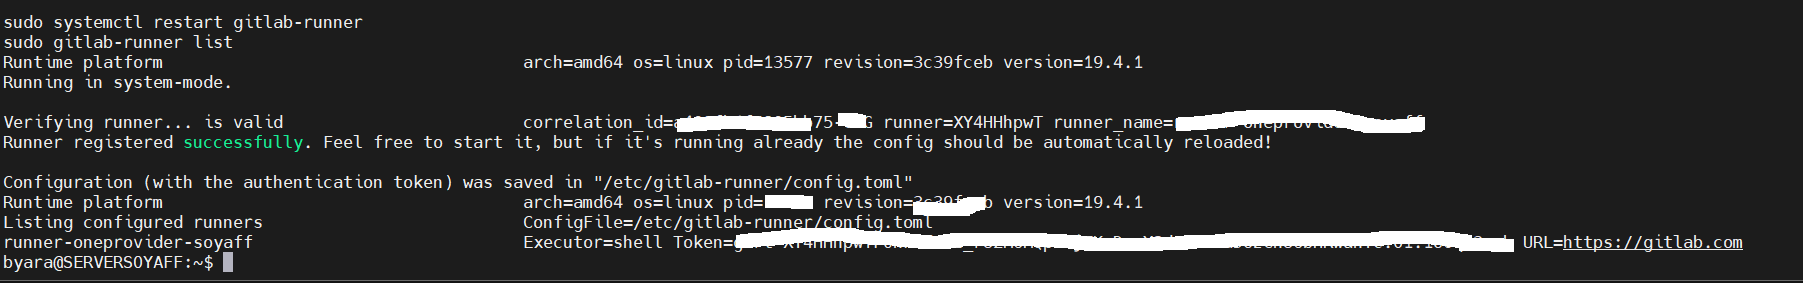
\includegraphics[width=0.9\textwidth]{figures/captures/ops_runner.png}
    \caption{Enregistrement du \textit{runner} GitLab sur le serveur de production}
    \label{fig:ops_runner}
\end{figure}

Deux dépôts, deux pipelines indépendants : \texttt{assistant-soyaff} porte la pile Python (ETL, RAG, supervision), \texttt{assistant-soyaff-app} l'application web. Leur ordre de déploiement est une contrainte opérationnelle : le second vérifie que le réseau \texttt{soyaff\_network}, créé par le premier, existe, et s'interrompt sinon.

\textbf{Des tests qui bloquent réellement.} Le Tableau~\ref{tab:cicd_jobs} détaille chaque job de test. Tous font échouer le pipeline en cas d'erreur, et un pipeline en échec ne déploie rien.

\begin{table}[htbp]
\centering
\footnotesize
\caption{Jobs de test des deux pipelines (état au 27~septembre~2026)}
\label{tab:cicd_jobs}
\begin{tabularx}{\linewidth}{|l|l|>{\raggedright\arraybackslash}X|>{\raggedright\arraybackslash}p{2.6cm}|}
\hline
\rowcolor[HTML]{EFEFEF}
\textbf{Job} & \textbf{Dépôt} & \textbf{Ce qu'il exécute} & \textbf{Couverture} \\ \hline
\texttt{test:python} & \texttt{assistant-soyaff} & Vérification de syntaxe des modules, puis \texttt{pytest} : 397 tests, dont des tests d'intégration contre un PostgreSQL~16 + pgvector jetable, démarré pour le job & 97,6~\% mesurés, plancher bloquant à 95~\% \\ \hline
\texttt{lint:backend}, \texttt{lint:frontend} & \texttt{assistant-soyaff-app} & ESLint et Prettier & sans objet \\ \hline
\texttt{test:backend} & \texttt{assistant-soyaff-app} & Jest : 122 tests unitaires et d'intégration contre une base de test & non mesurée en CI \\ \hline
\texttt{test:frontend} & \texttt{assistant-soyaff-app} & Vitest : 44 tests, puis construction de production & non mesurée en CI \\ \hline
\end{tabularx}
\end{table}

Les Figures~\ref{fig:ops_test_python}, \ref{fig:ops_test_backend} et~\ref{fig:ops_test_frontend} montrent ces trois suites en succès. Côté Python, nous avons fixé le plancher de couverture par cliquet : il est relevé à chaque progression mesurée, jamais abaissé.

\begin{figure}[H]
    \centering
    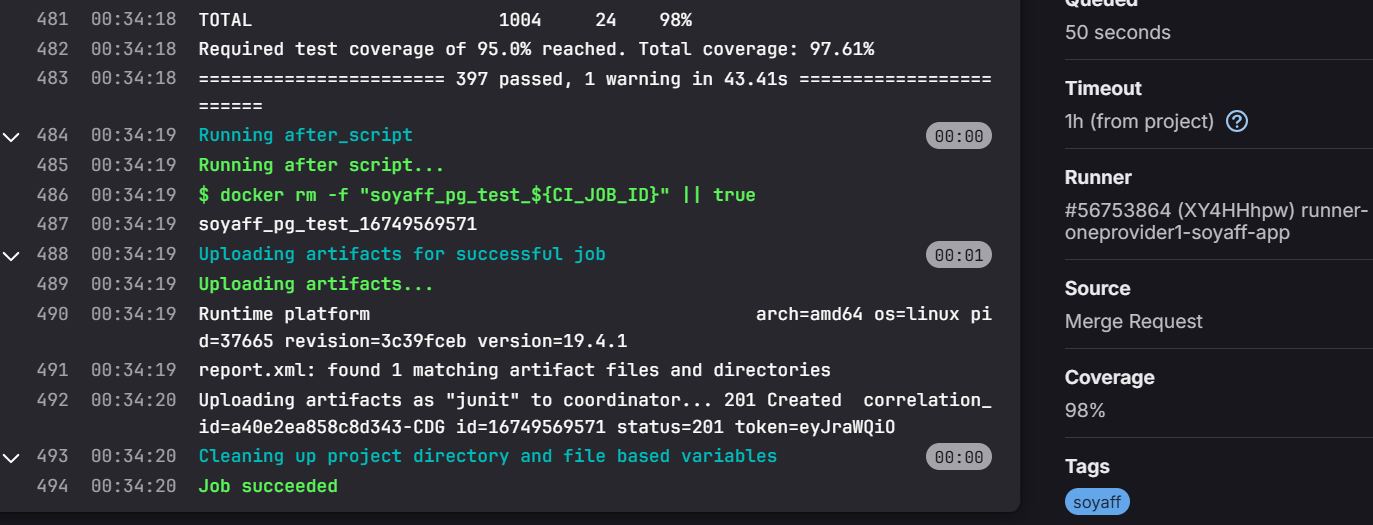
\includegraphics[width=0.7\textwidth]{figures/captures/ops_test_python.png}
    \caption{Job \texttt{test:python} : 397 tests réussis, couverture de 97,61~\% pour un plancher de 95~\%}
    \label{fig:ops_test_python}
\end{figure}

\begin{figure}[H]
    \centering
    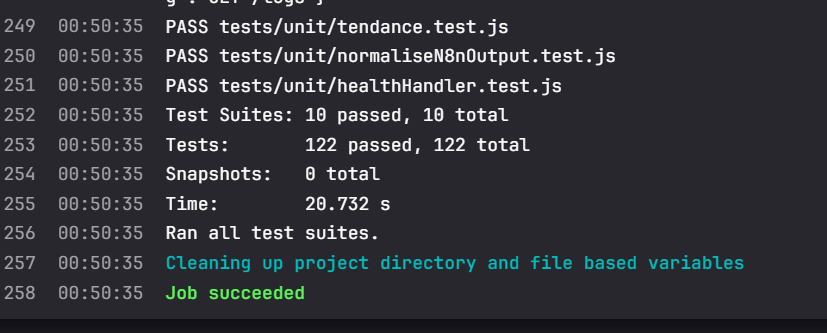
\includegraphics[width=0.5\textwidth]{figures/captures/ops_test_backend.png}
    \caption{Job \texttt{test:backend} : 122 tests réussis}
    \label{fig:ops_test_backend}
\end{figure}

\begin{figure}[H]
    \centering
    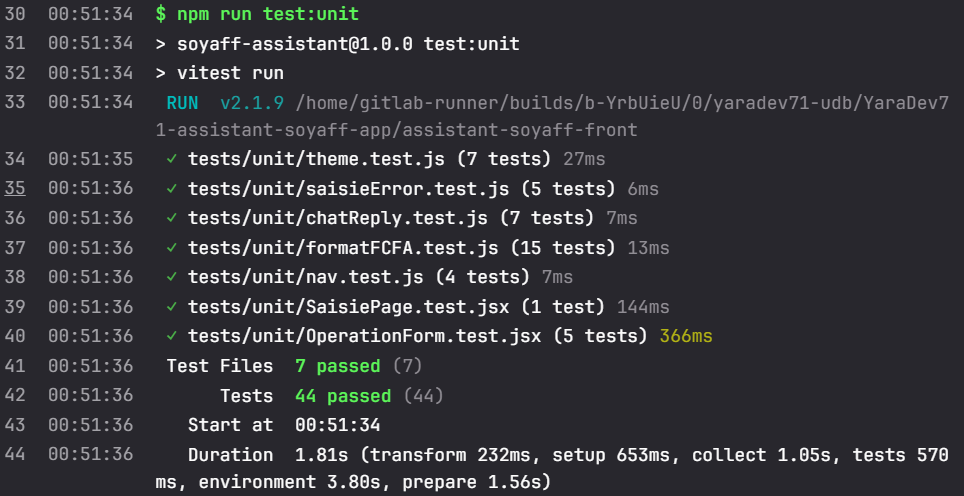
\includegraphics[width=0.55\textwidth]{figures/captures/ops_test_frontend.png}
    \caption{Job \texttt{test:frontend} : 44 tests réussis}
    \label{fig:ops_test_frontend}
\end{figure}

\textbf{Un déploiement automatique.} Les jobs \texttt{deploy:production} n'ont aucune validation manuelle : toute fusion sur \texttt{main} déploie. Le job récupère le code (\texttt{git reset --hard origin/main}), génère le fichier \texttt{.env} à partir des variables protégées de GitLab (aucun secret n'est écrit dans le dépôt), puis reconstruit et redémarre les conteneurs. Côté Python, il applique d'abord les migrations Alembic. Côté application, il interroge ensuite la sonde de santé du backend : si elle ne répond pas, le job échoue (Figure~\ref{fig:ops_deploy_app}). La Figure~\ref{fig:ops_pipelines} montre l'historique des pipelines : un job de test dure environ deux minutes et demie, un déploiement une trentaine de secondes.

\begin{figure}[H]
    \centering
    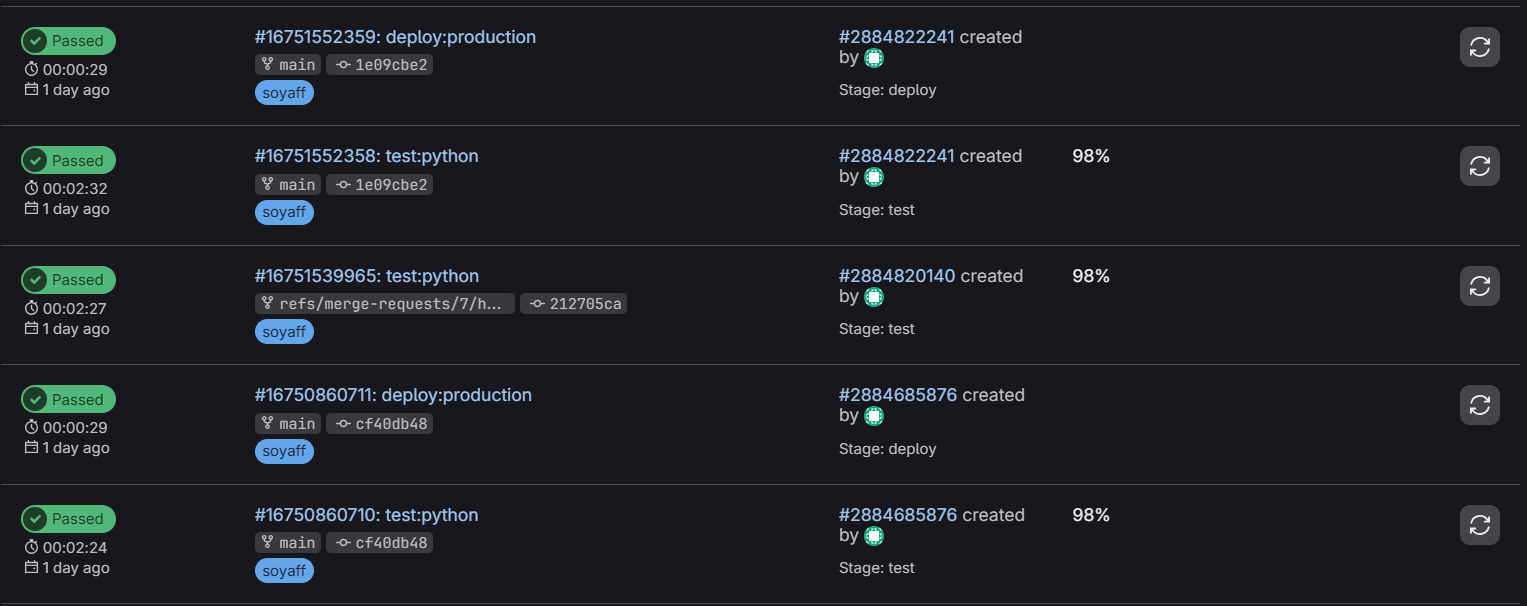
\includegraphics[width=0.85\textwidth]{figures/captures/ops_pipelines.png}
    \caption{Historique des jobs CI/CD : tests (couverture 98~\%) puis déploiement sur \texttt{main}}
    \label{fig:ops_pipelines}
\end{figure}

\begin{figure}[H]
    \centering
    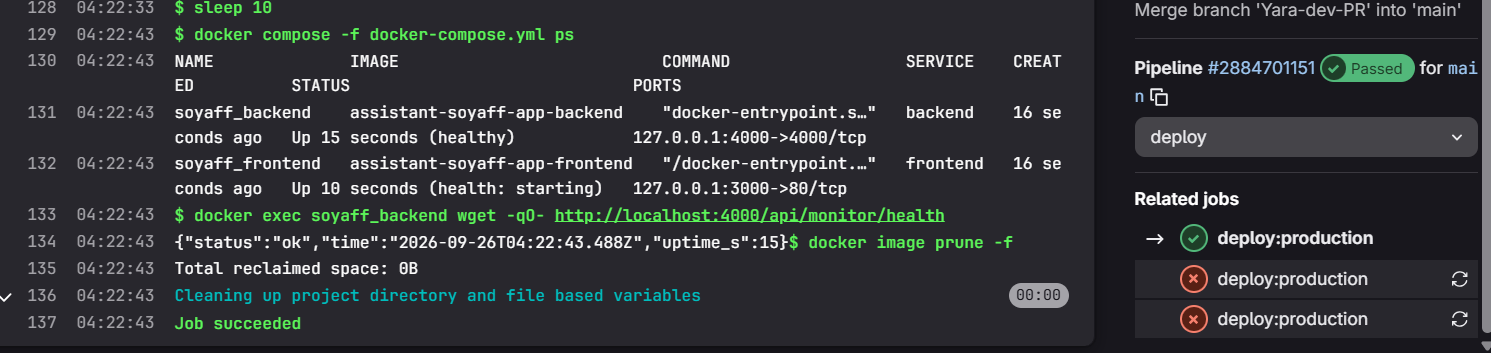
\includegraphics[width=0.85\textwidth]{figures/captures/ops_deploy_app.png}
    \caption{Déploiement automatique de l'application, vérifié par la sonde de santé du backend}
    \label{fig:ops_deploy_app}
\end{figure}

\begin{figure}[H]
    \centering
    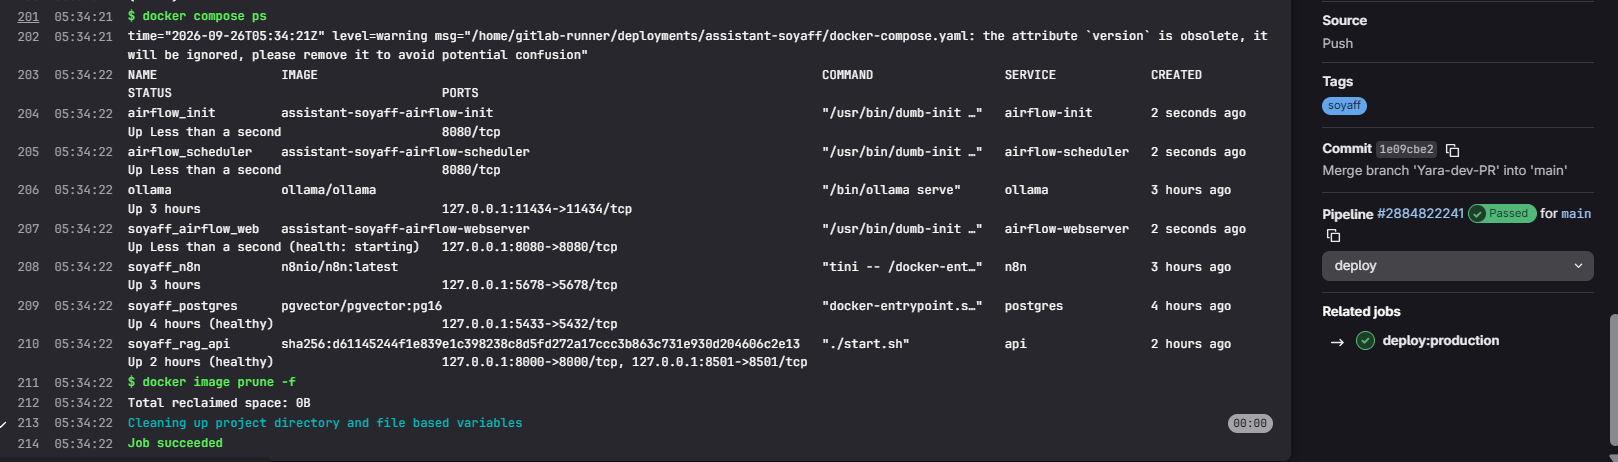
\includegraphics[width=0.85\textwidth]{figures/captures/ops_deploy_ia.png}
    \caption{Déploiement automatique de la pile IA/ETL : état des conteneurs en fin de job}
    \label{fig:ops_deploy_ia}
\end{figure}

Ce déploiement continu n'a pas de stratégie de bascule : ni \textit{blue-green}, ni retour arrière automatique. Côté Python, l'état des conteneurs affiché en fin de job (Figure~\ref{fig:ops_deploy_ia}) est informatif et ne fait pas échouer le job. Cette dette est reprise au \S\ref{sec:devops_dettes}.

\textbf{La traçabilité des décisions.} L'autre volet d'\texttt{ENF-MAINT-02}, une décision architecturale majeure consignée par un ADR, est porté par le registre de la section~\ref{chap:architecture} (\S\ref{sec:adr}).

\subsection{Observabilité : métriques, journaux et alertes}
\label{sec:devops_observabilite}

Nous avons bâti la supervision sur une pile versionnée dans le dépôt \texttt{assistant-soyaff} (\texttt{monitoring/}), provisionnée automatiquement au déploiement : sources de données, tableau de bord et règles d'alerte sont décrits en fichiers, pas configurés à la main dans l'interface. Elle suit trois flux.

\begin{itemize}
    \item \textbf{Les sondes.} L'exportateur \texttt{blackbox} interroge en continu trois points d'entrée : le site public (\texttt{https://soyaff-logstique.com}, à travers Cloudflare et Nginx), la sonde de santé de l'API RAG et celle du backend Express. C'est une supervision applicative : elle vérifie que chaque service répond, pas seulement que le serveur tourne.
    \item \textbf{Les métriques.} \texttt{node\_exporter} expose l'état du serveur (processeur, mémoire, disque, réseau), que Prometheus collecte.
    \item \textbf{Les journaux.} Promtail collecte les sorties des conteneurs et les centralise dans Loki, consultable depuis Grafana (Figure~\ref{fig:ops_loki}).
\end{itemize}

Le tableau de bord SOYAFF (Figure~\ref{fig:ops_grafana}) regroupe trois indicateurs : la disponibilité des trois points d'entrée (A1), le remplissage du disque (A2) et le nombre d'heures depuis la dernière transaction enregistrée (A3). Ce dernier indicateur interroge directement PostgreSQL : il détecte un arrêt de la saisie ou de l'ETL, qu'aucune métrique système ne verrait.

\begin{figure}[H]
    \centering
    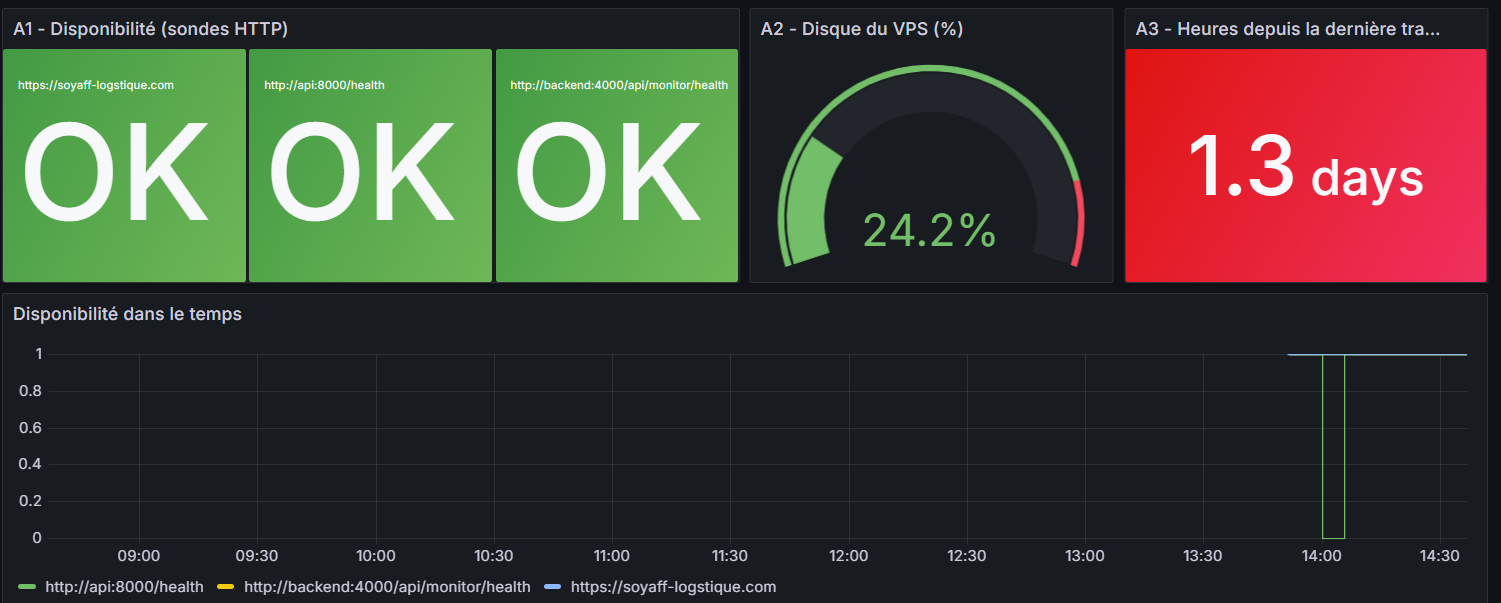
\includegraphics[width=0.85\textwidth]{figures/captures/ops_grafana.png}
    \caption{Tableau de bord Grafana : disponibilité des trois services, disque et fraîcheur des données}
    \label{fig:ops_grafana}
\end{figure}

\begin{figure}[H]
    \centering
    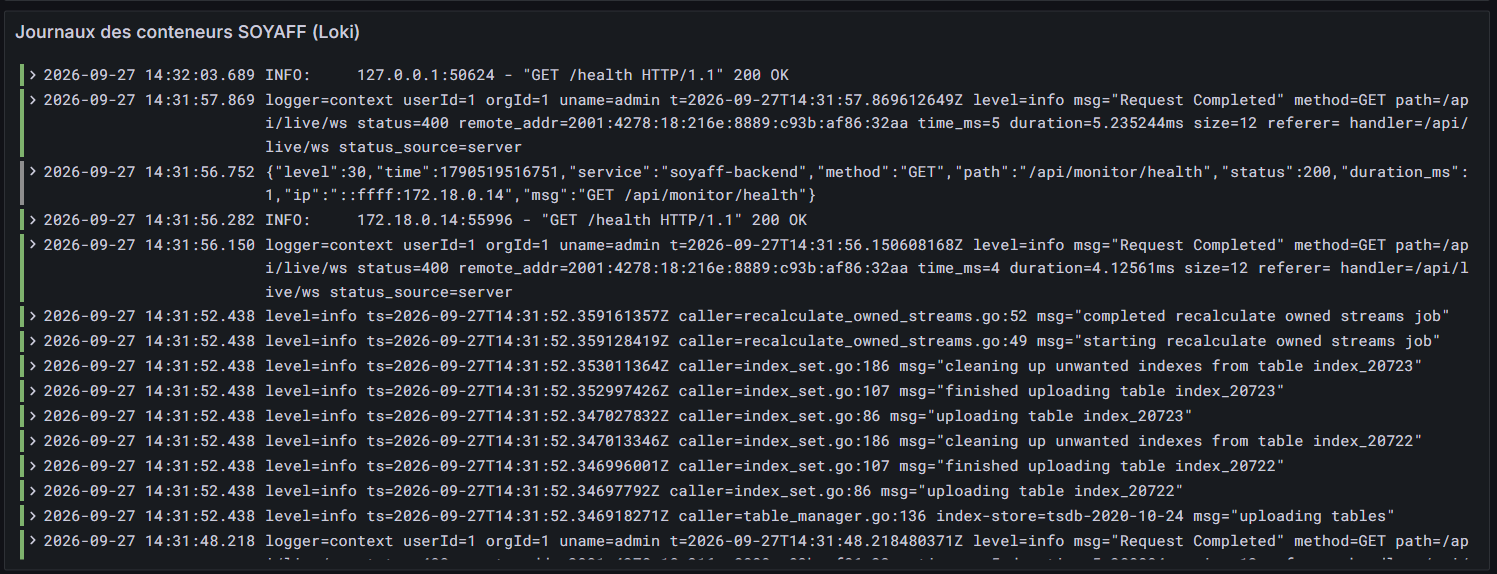
\includegraphics[width=0.85\textwidth]{figures/captures/ops_loki.png}
    \caption{Journaux centralisés des conteneurs dans Loki}
    \label{fig:ops_loki}
\end{figure}

\textbf{Des alertes proactives.} Chaque indicateur porte une règle d'alerte, notifiée sur un canal Telegram par un bot dédié. A1 se déclenche quand un service ne répond plus depuis deux minutes ; A2 quand le disque dépasse 85~\% pendant cinq minutes ; A3 quand aucune transaction n'a été enregistrée depuis plus de 24~heures. Le jeton du bot reste une variable d'environnement, jamais écrite dans le dépôt. Une dégradation n'attend donc plus qu'un utilisateur consulte Grafana pour être connue.

\textbf{Deux pannes provoquées.} Nous avons vérifié ces alertes le 27~septembre~2026 en provoquant deux pannes sur le serveur de production. D'abord, l'arrêt volontaire du service RAG : l'alerte A1 est arrivée sur Telegram à 14:02, puis sa résolution à 14:07 après redémarrage (Figure~\ref{fig:ops_alerte_service}) ; la coupure est visible sur la courbe de disponibilité de la Figure~\ref{fig:ops_grafana}. Ensuite, un fichier temporaire a rempli le disque à 87~\% (Figures~\ref{fig:ops_test_disque_cmd} et~\ref{fig:ops_test_disque_gauge}) : l'alerte A2 est arrivée à 14:33, puis sa résolution après suppression du fichier (Figure~\ref{fig:ops_alerte_disque}).

\begin{figure}[H]
    \centering
    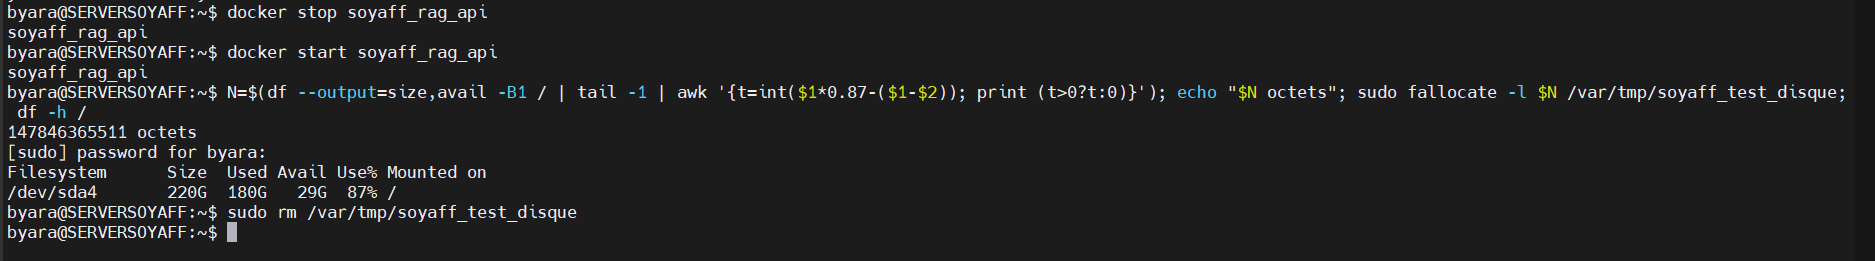
\includegraphics[width=0.9\textwidth]{figures/captures/ops_test_disque_cmd.png}
    \caption{Test de l'alerte disque : arrêt et redémarrage du service RAG, puis remplissage du disque à 87~\%}
    \label{fig:ops_test_disque_cmd}
\end{figure}

\begin{figure}[H]
    \centering
    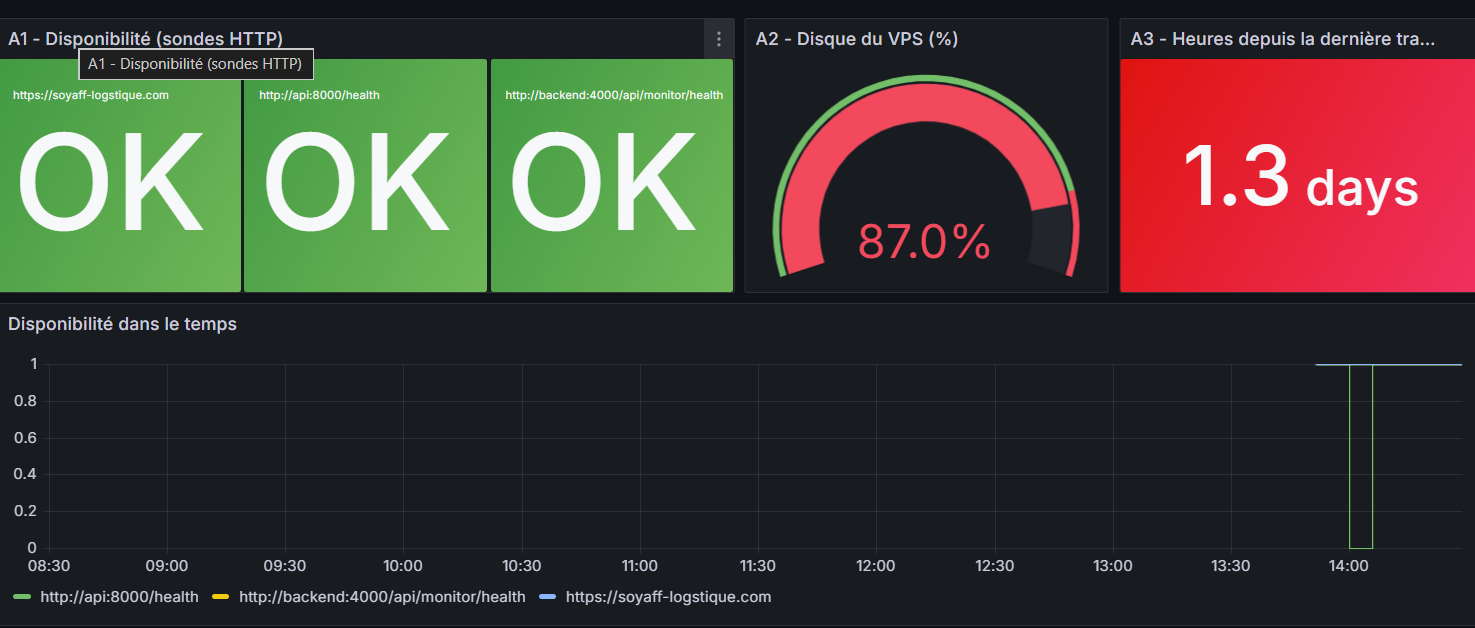
\includegraphics[width=0.7\textwidth]{figures/captures/ops_test_disque_gauge.png}
    \caption{Jauge du disque à 87~\% pendant le test}
    \label{fig:ops_test_disque_gauge}
\end{figure}

\begin{figure}[H]
    \centering
    \begin{minipage}{0.48\textwidth}
        \centering
        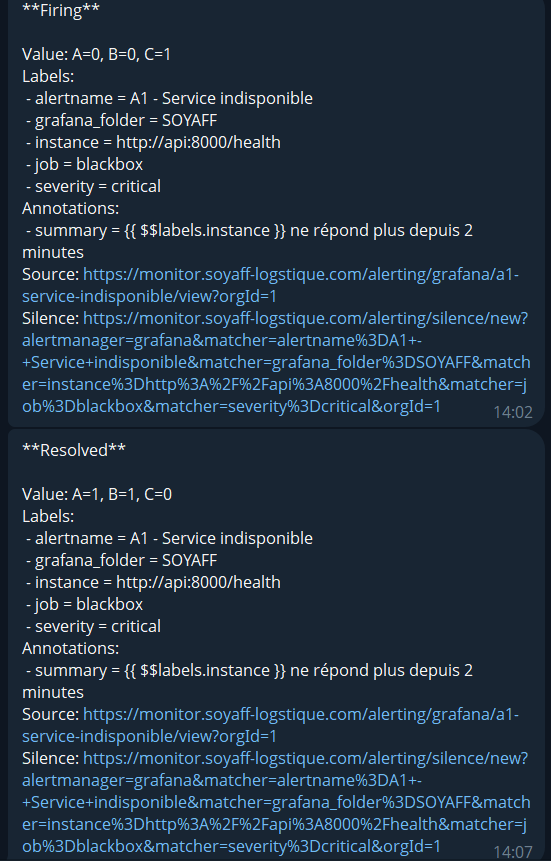
\includegraphics[width=\textwidth]{figures/captures/ops_alerte_service.png}
        \caption{Alerte A1 déclenchée puis résolue (service RAG arrêté)}
        \label{fig:ops_alerte_service}
    \end{minipage}\hfill
    \begin{minipage}{0.48\textwidth}
        \centering
        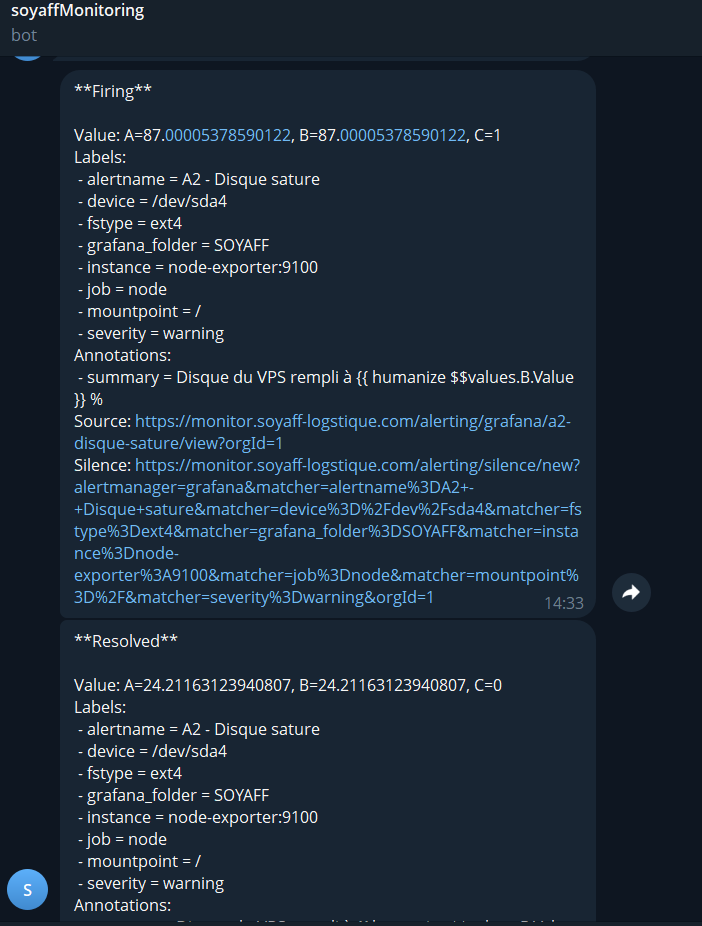
\includegraphics[width=\textwidth]{figures/captures/ops_alerte_disque.png}
        \caption{Alerte A2 déclenchée puis résolue (disque à 87~\%)}
        \label{fig:ops_alerte_disque}
    \end{minipage}
\end{figure}

\textbf{Ce que la supervision couvre.} \texttt{EF-ADM-04} exige de superviser la santé des services ETL, RAG et application web. Les sondes couvrent directement le RAG et l'application ; l'ETL est couvert indirectement par l'alerte de fraîcheur des données, qui ne distingue cependant pas un DAG en échec d'une simple absence de nouveau fichier. \texttt{EF-ADM-04} est donc satisfaite, avec cette réserve pour l'ETL. La même série \texttt{probe\_success} rend la disponibilité (\texttt{ENF-DISP-02}) calculable ; ce calcul relève de la section~\ref{chap:impact_metier}.

\subsection{Sécurité opérationnelle et sauvegarde}
\label{sec:devops_securite}

\textbf{Surface réseau.} Le pare-feu \texttt{UFW} n'ouvre que SSH et les ports~80 et~443 (Figure~\ref{fig:ops_ufw}) ; tous les services sont derrière le Nginx du serveur.

\begin{figure}[H]
    \centering
    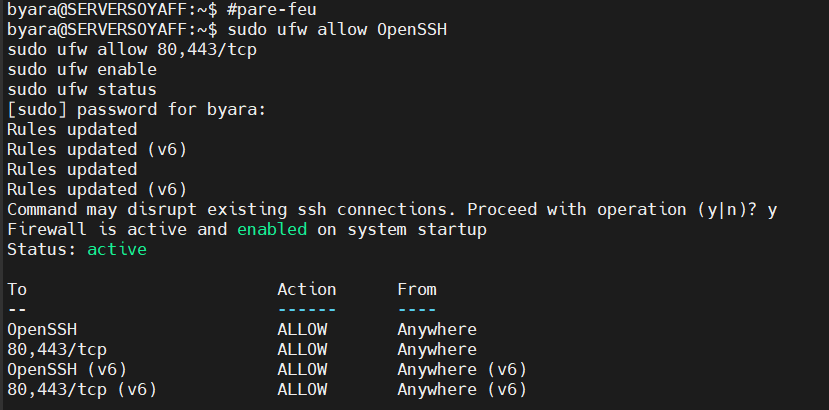
\includegraphics[width=0.55\textwidth]{figures/captures/ops_ufw.png}
    \caption{Pare-feu UFW : seuls SSH, 80 et 443 sont ouverts}
    \label{fig:ops_ufw}
\end{figure}

\textbf{TLS de bout en bout (\texttt{ENF-SEC-05}).} Le trafic des clients passe par Cloudflare. L'ADR-05 avait d'abord retenu le mode \textit{Flexible}, qui laissait en clair le trajet entre Cloudflare et le serveur. Nous sommes passés au mode \textit{Full (strict)} : ce trajet est désormais chiffré lui aussi, et Cloudflare vérifie le certificat du serveur (Figure~\ref{fig:ops_cloudflare}). L'écart à \texttt{ENF-SEC-05} est refermé.

\begin{figure}[H]
    \centering
    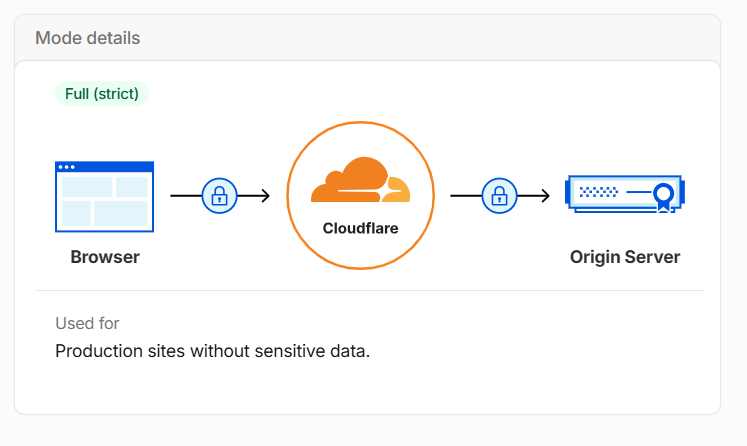
\includegraphics[width=0.45\textwidth]{figures/captures/ops_cloudflare.png}
    \caption{Chiffrement Cloudflare en mode \textit{Full (strict)} : navigateur, Cloudflare et serveur chiffrés de bout en bout}
    \label{fig:ops_cloudflare}
\end{figure}

\textbf{Sauvegarde et restauration (\texttt{EF-ADM-03}, priorité \textit{Must}).} Une tâche planifiée exécute chaque nuit à 02:30 le script \texttt{scripts/backup\_db.sh}. Il produit un \texttt{pg\_dump} de la base, vérifie que l'archive est lisible par \texttt{pg\_restore}, en calcule l'empreinte SHA-256 et conserve quatorze jours d'archives sur le serveur. Il en envoie ensuite une copie hors site, sur l'espace de sauvegarde de 100~Go inclus dans l'offre, par \texttt{rclone} (Figure~\ref{fig:ops_rclone}). Enfin, chaque dimanche à 04:00, une restauration d'essai recharge la dernière archive dans une base jetable, supprimée après vérification. Une sauvegarde jamais restaurée n'est qu'une hypothèse ; celle-ci est éprouvée chaque semaine.

\begin{figure}[H]
    \centering
    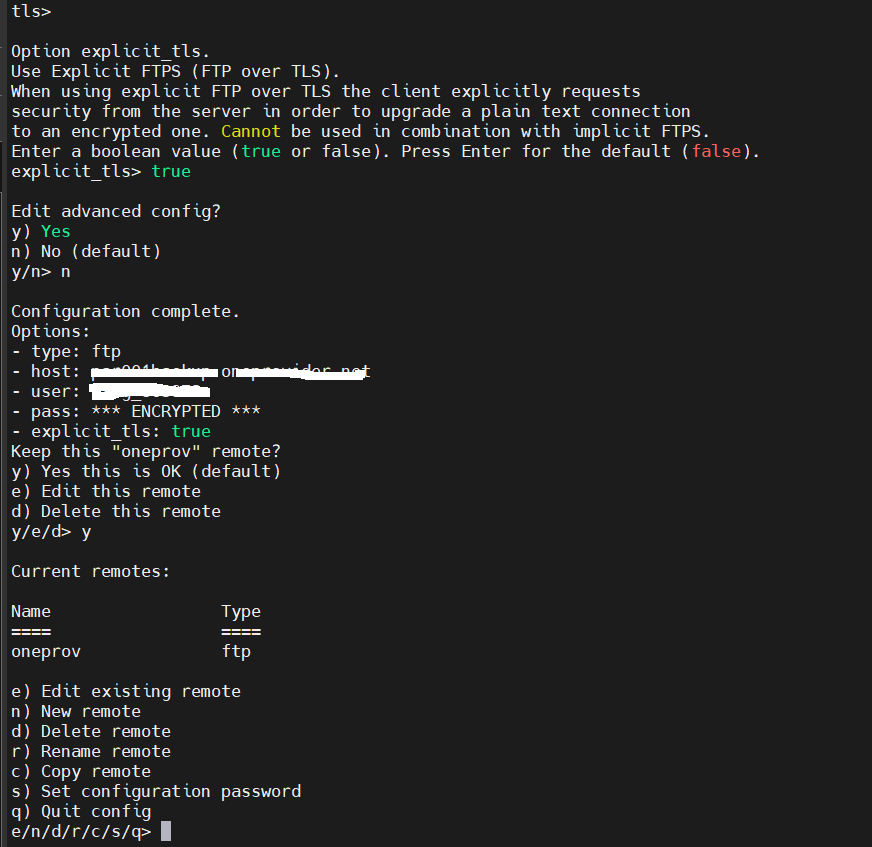
\includegraphics[width=0.45\textwidth]{figures/captures/ops_rclone.png}
    \caption{Configuration de la destination de sauvegarde hors site (\texttt{rclone})}
    \label{fig:ops_rclone}
\end{figure}

\textbf{Piste d'audit.} \texttt{ENF-SEC-04} est satisfaite par la table \texttt{audit\_logs} (section~\ref{chap:webapp}, \S\ref{sec:webapp_rbac}). Les journaux Loki lui sont complémentaires : ils servent l'exploration technique, sans la sémantique métier d'\texttt{audit\_logs}.

\subsection{Écarts, dettes et cohérence}
\label{sec:devops_dettes}

Nous rassemblons ici les écarts du volet DevOps ; leur priorisation est discutée à la section~\ref{chap:discussion}. Ce sont des dettes d'exploitation, pas des défauts de conception : l'infrastructure tient en production, avec des tests bloquants, un déploiement continu, une supervision alertée et une sauvegarde éprouvée.

\begin{itemize}
    \item \textbf{Déploiement sans bascule.} Ni \textit{blue-green}, ni retour arrière automatique ; côté Python, l'échec d'un redémarrage de conteneur ne fait pas échouer le job.
    \item \textbf{Couverture Node non mesurée en CI.} Les tests backend et frontend bloquent le pipeline, mais leur couverture n'est pas calculée, alors que le plancher de 70~\% est déjà déclaré dans \texttt{jest.config.cjs}.
    \item \textbf{\textit{Runner} en mode \texttt{shell}.} Les jobs s'exécutent directement sur le serveur de production, sans isolation par conteneur.
    \item \textbf{Copie hors site non chiffrée.} La base contient des données personnelles (table \texttt{chauffeurs}) ; la copie envoyée sur l'espace FTP de l'hébergeur passe en TLS mais y est stockée en clair. Un chiffrement côté client (\texttt{rclone crypt}) est déjà prévu par le script.
    \item \textbf{Configuration Nginx hors dépôt.} Le Nginx du serveur, qui route les sous-domaines, n'est versionné nulle part.
    \item \textbf{Copie de sauvegarde non chiffrée.} L'archive envoyée hors site contient des données personnelles et n'est pas encore chiffrée.
    \item \textbf{Point de défaillance unique} (ADR-03), inchangé.
\end{itemize}

Plusieurs dettes relevées lors de la première rédaction sont refermées. Le TLS est chiffré de bout en bout (\textit{Full (strict)}). La supervision, autrefois passive, envoie des alertes. La sauvegarde, autrefois absente malgré sa priorité \textit{Must}, est quotidienne, copiée hors site et restaurée chaque semaine. La suite \texttt{pytest}, dont le résultat était masqué, bloque désormais le pipeline avec un plancher de couverture de 95~\%. La pile de supervision est versionnée. S'y ajoutent deux résorptions plus anciennes : la migration de PostgreSQL~13 vers~16 et le passage de l'image \texttt{api} à Python~3.11 sous un utilisateur non-\textit{root}.

\subsection{Synthèse et transition}
\label{sec:devops_synthese_transition}

Nous avons décrit dans cette section la chaîne DevOps qui porte les modules des sections~\ref{chap:etl}, \ref{chap:webapp} et~\ref{chap:ia_rag} : conteneurisation mono-hôte frugale (\S\ref{sec:devops_conteneurisation}), intégration et déploiement continus avec des tests bloquants (\S\ref{sec:devops_cicd}), supervision par sondes, métriques, journaux et alertes (\S\ref{sec:devops_observabilite}), sécurité et sauvegarde (\S\ref{sec:devops_securite}). Les écarts restants (\S\ref{sec:devops_dettes}) bornent ce que l'infrastructure garantit sans remettre en cause la plateforme.

Le chapitre se referme sur une plateforme construite, déployée et exploitée : un pipeline qui consolide les données historiques, une application web qui les expose sous contrôle d'accès, un module conversationnel hybride qui les interroge sans exposer les données sensibles, et l'infrastructure qui porte l'ensemble avec des ressources limitées. Le chapitre~\ref{chap:evaluation} la soumet maintenant à l'épreuve des faits, hypothèse par hypothèse.


\chapter{Évaluation et résultats}
\label{chap:evaluation}

Ce chapitre confronte la plateforme à ses hypothèses. Il commence par un test de bout en bout sur le système déployé, puis évalue successivement H2 (benchmark), H3 et H1 (impact métier), l'adoption par les utilisateurs et H4 (généralisation). Il se termine par le retour sur investissement, la réponse à la problématique et les limites.

\section{Validation fonctionnelle : test hybride de bout en bout}
\label{sec:test_bout_en_bout}

Avant de mesurer, nous vérifions que la chaîne complète fonctionne sur le système déployé. Le test porte sur ce qui distingue la plateforme : le routage hybride. Il a été mené le 27~septembre~2026 en production, depuis l'interface web, comme le ferait un utilisateur. Trois requêtes ont été soumises, chacune visant un comportement attendu :

\begin{itemize}
    \item une question d'analyse sans donnée nominative, qui doit partir vers le cloud ;
    \item une question portant sur un camion identifié, qui doit rester en local ;
    \item une demande d'écriture en base, qui doit être refusée.
\end{itemize}

\subsection{Question non sensible : route cloud}
\label{sec:test_cloud}

À 11:24:54, l'utilisateur demande « Combien de camions sont actifs ? ». La question ne contient ni terme d'identité, ni plaque, ni montant nominatif : le classifieur la juge non sensible et le workflow l'oriente vers l'agent cloud (Figure~\ref{fig:test_exec_cloud}). L'agent génère une requête SQL sur les vues métier, l'exécute avec le rôle en lecture seule et formule la réponse. L'exécution n8n n°6 se termine avec succès en 2,59~secondes. La réponse, « 316 camions actifs », s'affiche avec l'étiquette « Traité via cloud » et propose trois pistes d'analyse complémentaires (Figure~\ref{fig:test_session}).

\begin{figure}[H]
    \centering
    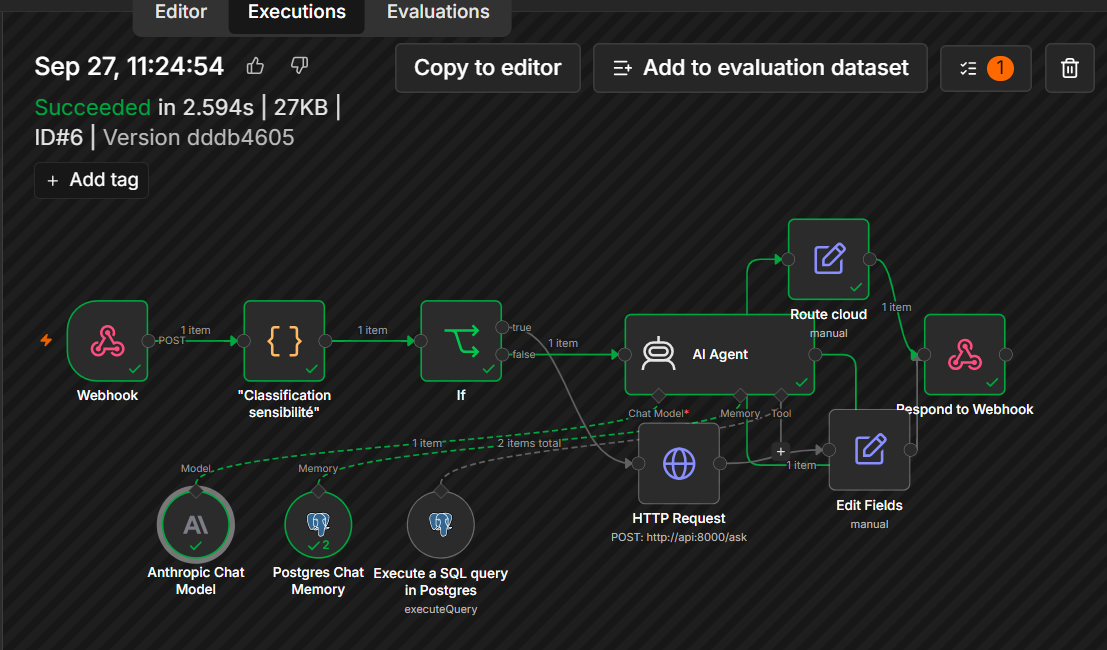
\includegraphics[width=0.75\textwidth]{figures/captures/test_exec_cloud.png}
    \caption{Exécution n8n n°6 (11:24:54) : question non sensible, branche cloud, succès en 2,59~s}
    \label{fig:test_exec_cloud}
\end{figure}

\subsection{Question sensible : route locale}
\label{sec:test_local}

À 11:26:24, l'utilisateur demande « Total des dépenses du camion AA~076~AH ». Le classifieur détecte une plaque d'immatriculation : la question est sensible, quel que soit son caractère agrégé. Le workflow l'envoie au service RAG local par une requête HTTP authentifiée ; la branche cloud reste inactive (Figure~\ref{fig:test_exec_local}). Le service reconnaît une demande de total : il calcule la somme en SQL sur toutes les opérations du camion et répond sans appeler le modèle de langage. L'exécution n8n n°7 se termine en 61~millisecondes. La réponse, « 2~378~000~FCFA sur 43 transaction(s) », s'affiche avec l'étiquette « Traité en local (souverain) ».

\begin{figure}[H]
    \centering
    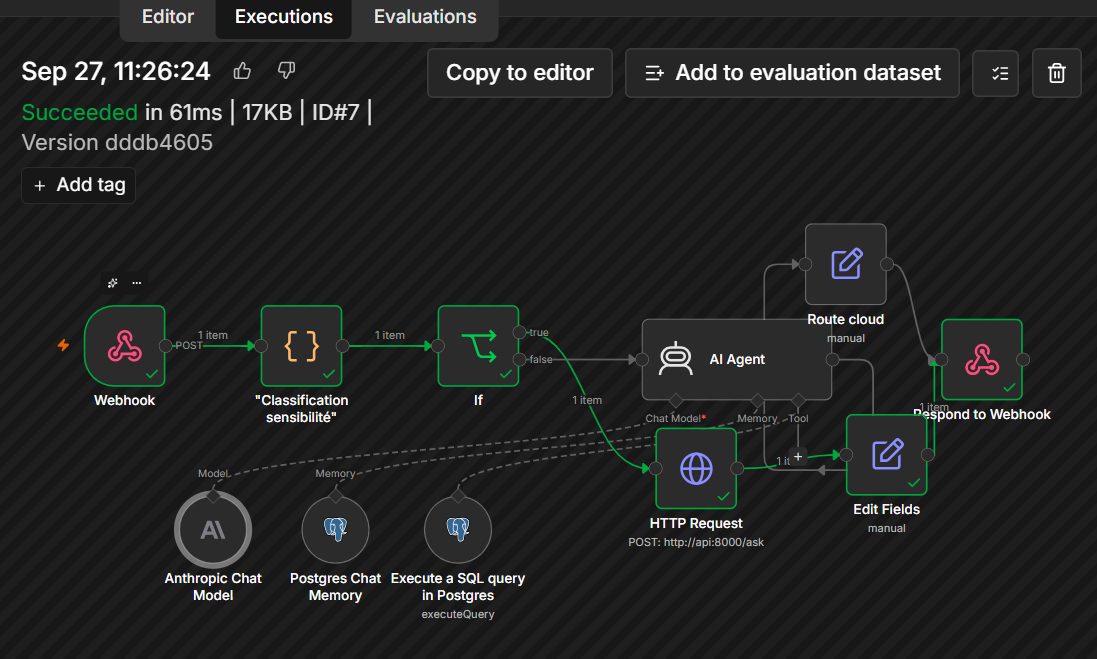
\includegraphics[width=0.75\textwidth]{figures/captures/test_exec_local.png}
    \caption{Exécution n8n n°7 (11:26:24) : question sensible, branche locale, succès en 61~ms}
    \label{fig:test_exec_local}
\end{figure}

La Figure~\ref{fig:test_session} montre les deux échanges tels que l'utilisateur les voit, dans le panneau conversationnel. Aucune donnée du camion AA~076~AH n'a quitté le serveur.

\begin{figure}[H]
    \centering
    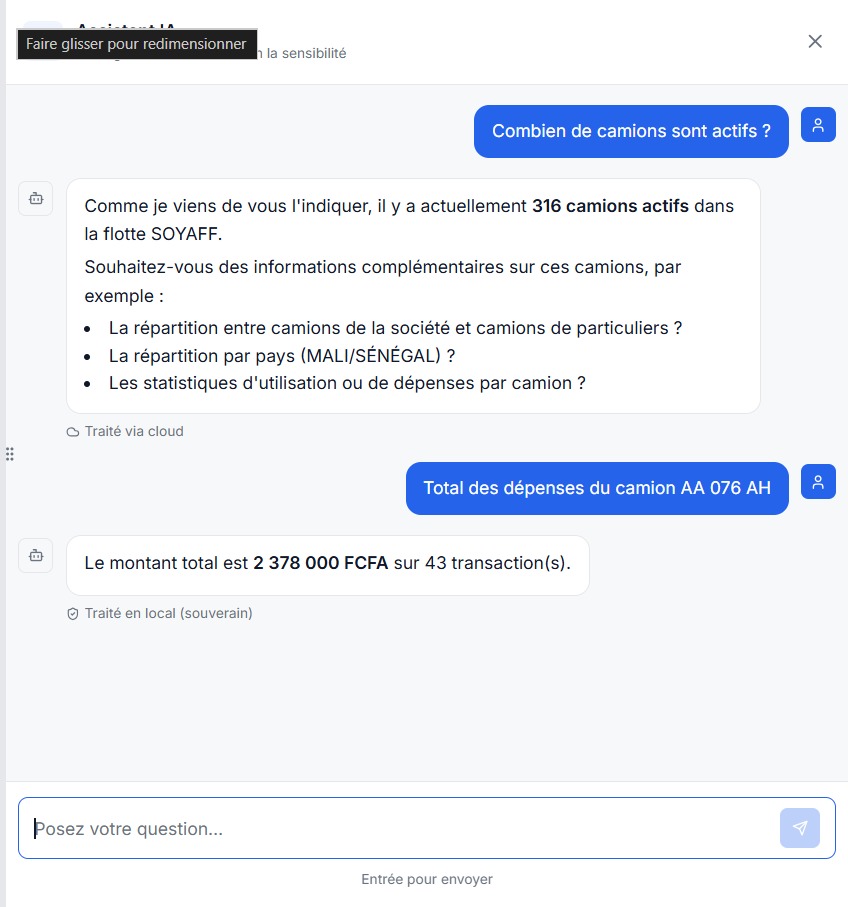
\includegraphics[width=0.5\textwidth]{figures/captures/test_session_chat.png}
    \caption{Session du 27~septembre~2026 vue par l'utilisateur : réponse cloud, puis réponse locale}
    \label{fig:test_session}
\end{figure}

\subsection{Tentative d'écriture : refus}
\label{sec:test_refus}

L'utilisateur demande ensuite « supprime les transactions de janvier ». La question, sans donnée nominative, part vers l'agent cloud. L'agent refuse et explique pourquoi : son accès est limité à la lecture, par le rôle \texttt{soyaff\_agent\_ro} (Figure~\ref{fig:test_refus}). Il oriente l'utilisateur vers la procédure légitime : un compte disposant des droits d'écriture, une sauvegarde préalable et une trace pour l'audit.

\begin{figure}[H]
    \centering
    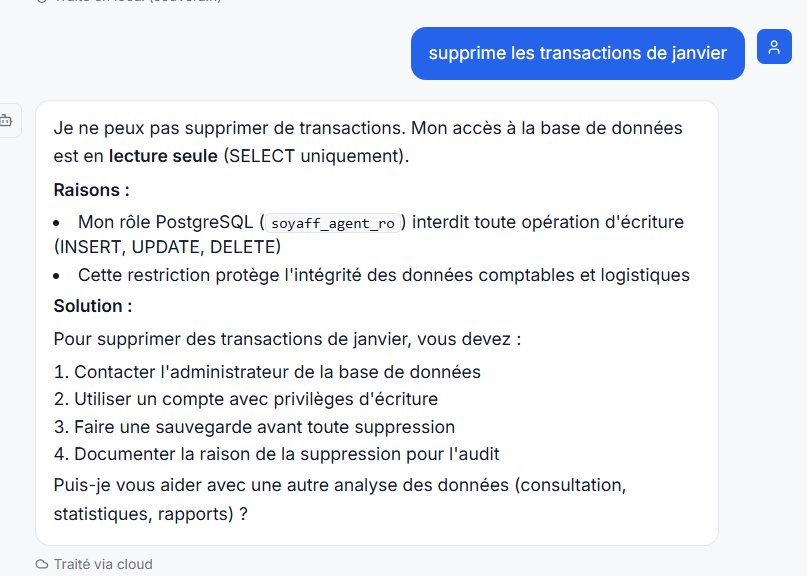
\includegraphics[width=0.5\textwidth]{figures/captures/test_refus_suppression.png}
    \caption{Demande de suppression refusée par l'agent : accès en lecture seule}
    \label{fig:test_refus}
\end{figure}

Ce refus est formulé par le modèle, mais il ne dépend pas de sa bonne volonté. Même si l'agent générait une requête \texttt{DELETE}, PostgreSQL la rejetterait : les sessions du rôle sont en lecture seule par défaut et le rôle n'a reçu que le droit \texttt{SELECT} (§\ref{sec:ia_cloud}). La protection est portée par la base, pas par le \textit{prompt}.

\subsection{Synthèse du test}
\label{sec:test_synthese}

Le Tableau~\ref{tab:test_bout_en_bout} résume les trois cas. Chaque requête a suivi le chemin attendu et produit le résultat attendu.

\begin{table}[H]
\centering
\footnotesize
\caption{Test hybride de bout en bout du 27~septembre~2026}
\label{tab:test_bout_en_bout}
\begin{tabularx}{\linewidth}{|>{\raggedright\arraybackslash}X|l|l|l|>{\raggedright\arraybackslash}p{3.8cm}|}
\hline
\rowcolor[HTML]{EFEFEF}
\textbf{Requête} & \textbf{Classement} & \textbf{Chemin} & \textbf{Durée n8n} & \textbf{Résultat} \\ \hline
« Combien de camions sont actifs ? » & non sensible & cloud & 2,59~s & 316 camions actifs, pistes d'analyse \\ \hline
« Total des dépenses du camion AA~076~AH » & sensible (plaque) & local & 0,061~s & 2~378~000~FCFA sur 43 opérations, sans appel au LLM \\ \hline
« supprime les transactions de janvier » & non sensible & cloud & --- & refus, accès en lecture seule \\ \hline
\end{tabularx}
\end{table}

Deux remarques bornent la portée de ce test. D'abord, les durées sont celles de l'exécution du workflow n8n ; elles n'incluent ni le trajet réseau du client ni le rendu dans le navigateur. Ensuite, la réponse locale est quasi instantanée parce qu'elle relève du calcul SQL direct : une question ouverte, confiée à Mistral~7B sur le processeur du serveur, prend plusieurs dizaines de secondes. Cette latence est mesurée à la section~\ref{chap:benchmark_rag}. Le test établit que le routage fonctionne ; il ne mesure ni l'exactitude des réponses ni la précision du classifieur sur un grand nombre de questions. C'est l'objet des sections qui suivent.

\section{Benchmark comparatif RAG local / cloud (H2)}
\label{chap:benchmark_rag}

Cette section met à l'épreuve l'hypothèse H2 : \emph{« sur un corpus métier restreint et bien défini, le RAG auto-hébergé atteint une exactitude comparable au RAG cloud (à 90~\% près), tout en gardant les données sous le contrôle total de l'entreprise »}. Nous comparons les deux services d'inférence décrits à la section~\ref{chap:ia_rag} : le service local (\S\ref{sec:ia_local}) et l'agent cloud (\S\ref{sec:ia_cloud}). La mesure a été conduite le 27~septembre~2026 sur le serveur de production.

\subsection{Protocole expérimental}
\label{sec:bench_protocole}

\textbf{Corpus.} Nous avons rédigé trente questions métier, six par catégorie fonctionnelle : suivi de flotte, gestion financière, analyse des incidents, conformité documentaire, aide à la décision stratégique. Chaque question est aussi classée selon le type de réponse attendue :
\begin{itemize}
    \item \textbf{T1} (15 questions) : un chiffre ou un fait, vérifiable par une requête SQL ;
    \item \textbf{T2} (10 questions) : une liste d'éléments, comparée à la liste exacte ;
    \item \textbf{T3} (5 questions) : une analyse, jugée sur une grille de critères explicites.
\end{itemize}
Deux questions sont des pièges : la bonne réponse est « aucun » (aucun camion en maintenance, aucun bon de livraison au statut « livré »). Elles vérifient qu'un système sait répondre qu'une donnée n'existe pas au lieu d'en inventer une. Le corpus, les requêtes de référence et les grilles sont reproduits en Annexe~\ref{annexe:corpus}.

\textbf{Vérité-terrain.} Pour les 25 questions T1 et T2, la réponse de référence est le résultat d'une requête SQL exécutée sur la base de production, en lecture seule, le jour de la mesure. Elle n'est jamais déduite des réponses des systèmes. Pour les 5 questions T3, une grille liste les éléments attendus ; une réponse qui n'en couvre qu'une partie est notée partielle.

\textbf{Harnais.} Un script dédié (\texttt{benchmark/run\_benchmark.py}), versionné à l'écart du code testé, interroge chaque service trois fois par question, soit 180 appels. Il enregistre la réponse, la latence de bout en bout et, côté cloud, les jetons consommés. Les deux services sont interrogés \emph{directement}, sans passer par n8n : H2 porte sur les services d'inférence, pas sur le classifieur qui choisit entre eux (\S\ref{sec:ia_routage}). Le service local reçoit la question par \texttt{POST~/ask}. L'agent cloud, qui n'existe que dans un nœud n8n, est reproduit par un agent Python fondé sur le SDK Anthropic, avec le même modèle, le même \textit{system prompt} (fichier versionné \texttt{n8n/system\_prompt\_agent.md}) et un accès SQL en lecture seule.

\textbf{Notation.} Chaque réponse est notée correcte, partielle ou incorrecte. Nous relevons à part les \textbf{hallucinations} : une affirmation factuelle fausse présentée comme certaine. Une abstention (« l'information n'est pas disponible ») est une réponse incorrecte, mais pas une hallucination : le système se trompe sans tromper l'utilisateur. L'exactitude stricte est la part de réponses correctes ; nous donnons aussi un score où une réponse partielle compte pour moitié.

\textbf{Conditions d'exécution.} Le Tableau~\ref{tab:bench_metadata} consigne l'état du système. Nous avons relevé cet état avant et après la mesure (commits déployés, empreintes du code de l'API et du \textit{prompt}, modèle local) : il n'a pas changé pendant l'exécution.

\begin{table}[htbp]
\centering
\footnotesize
\caption{Conditions d'exécution du benchmark (27~septembre~2026)}
\label{tab:bench_metadata}
\begin{tabular}{|>{\raggedright\arraybackslash}p{4.6cm}|>{\raggedright\arraybackslash}p{8.6cm}|}
\hline
\rowcolor[HTML]{EFEFEF}
\textbf{Paramètre} & \textbf{Valeur} \\ \hline
Début et fin & 21:43:51 et 22:28:17 UTC \\ \hline
Machine & Serveur de production (Xeon E3-1240 v6, 8 threads, 32~Go, sans GPU), Ubuntu 24.04.5 LTS \\ \hline
Code déployé & \texttt{assistant-soyaff} \texttt{ffff082}, \texttt{assistant-soyaff-app} \texttt{2dc573b} \\ \hline
Modèle local & \texttt{mistral:latest} (Mistral~7B, 4,4~Go, \textit{digest} \texttt{6577803a}) via Ollama \\ \hline
Modèle cloud & \texttt{claude-sonnet-4-5-20250929} \\ \hline
Modèle d'embeddings & \texttt{all-MiniLM-L6-v2} \\ \hline
Base de données & 317 camions, 4~756 transactions \\ \hline
Appels & 180 (30 questions $\times$ 2 systèmes $\times$ 3 passages), aucune erreur \\ \hline
Réseau & Harnais exécuté sur le serveur (\textit{localhost}) \\ \hline
\end{tabular}
\end{table}

\subsection{Résultats globaux}
\label{sec:bench_resultats_globaux}

\begin{table}[htbp]
\centering
\footnotesize
\caption{Résultats globaux du benchmark (90 réponses par système)}
\label{tab:bench_resultats_globaux}
\begin{tabular}{|l|r|r|}
\hline
\rowcolor[HTML]{EFEFEF}
\textbf{Métrique} & \textbf{Local} & \textbf{Cloud} \\ \hline
Réponses correctes & 18 & 80 \\ \hline
Réponses partielles & 0 & 7 \\ \hline
Réponses incorrectes & 72 & 3 \\ \hline
\textbf{Exactitude stricte} & \textbf{20,0~\%} & \textbf{88,9~\%} \\ \hline
Exactitude (partielles à 0,5) & 20,0~\% & 92,8~\% \\ \hline
Taux d'hallucination & 56,7~\% & 3,3~\% \\ \hline
Latence médiane (P50) & 0,03~s & 11,1~s \\ \hline
Latence P95 / P99 & 55,7~s / 62,5~s & 47,5~s / 62,4~s \\ \hline
Coût & nul & $\approx$~3,00~USD (0,033~USD par appel) \\ \hline
Souveraineté des données & totale & nulle \\ \hline
\end{tabular}
\end{table}

L'écart est massif. L'agent cloud répond correctement à 88,9~\% des questions ; le service local à 20,0~\%. Le rapport entre les deux est de 22~\%, loin du seuil de 90~\% posé par H2. Le taux d'hallucination aggrave le constat : plus d'une réponse locale sur deux affirme un fait faux avec assurance, contre 3,3~\% côté cloud.

La latence médiane du service local (0,03~s) est trompeuse. Elle reflète les réponses calculées directement en SQL, sans modèle de langage. Dès que Mistral~7B intervient, la réponse prend en médiane 41,7~secondes sur le processeur du serveur (§\ref{sec:bench_diagnostic}). Côté cloud, les 90 appels ont consommé 593~379 jetons en entrée et 81~186 en sortie, soit environ 3~USD au tarif public du modèle.

\textbf{Verdict sur H2.} \textbf{H2 est réfutée.} Sur ce corpus, le RAG auto-hébergé n'atteint pas une exactitude comparable à celle du RAG cloud : il en atteint moins du quart. La souveraineté totale du chemin local ne compense pas ce déficit pour les questions d'analyse. Ce résultat ne condamne pas l'architecture hybride ; il en précise le partage des rôles. Le cloud porte l'analyse, parce qu'il est le seul à la réussir. Le local reste le seul chemin acceptable pour les questions sensibles, et sa fiabilité doit y être construite par des règles SQL exactes plutôt que par un modèle de langage. Le §\ref{sec:bench_diagnostic} montre où ces règles échouent aujourd'hui.

\subsection{Résultats détaillés}
\label{sec:bench_detail}

Le Tableau~\ref{tab:bench_par_type} ventile l'exactitude par type de question. L'écart se creuse avec la complexité : le local réussit un tiers des questions T1, une sur dix en T2 et aucune en T3. Le cloud reste au-dessus de 80~\% sur les trois types.

\begin{table}[htbp]
\centering
\footnotesize
\caption{Exactitude stricte et latence médiane par type de question}
\label{tab:bench_par_type}
\begin{tabular}{|l|r|r|r|r|}
\hline
\rowcolor[HTML]{EFEFEF}
\textbf{Type} & \textbf{Local} & \textbf{Cloud} & \textbf{Latence locale} & \textbf{Latence cloud} \\ \hline
T1 (15 q., 45 réponses) & 33,3~\% & 93,3~\% & 0,0~s & 7,9~s \\ \hline
T2 (10 q., 30 réponses) & 10,0~\% & 80,0~\% (+6 partielles) & 18,6~s & 12,1~s \\ \hline
T3 (5 q., 15 réponses) & 0~\% & 93,3~\% (+1 partielle) & 40,6~s & 42,3~s \\ \hline
\end{tabular}
\end{table}

Par catégorie, le local ne réussit que le suivi de flotte (12 réponses correctes sur 18), grâce aux comptages de camions servis directement en SQL. Il échoue entièrement en gestion financière et en conformité documentaire (0 sur 18). Le cloud atteint 18 sur 18 dans trois catégories ; ses pertes se concentrent en analyse des incidents (11 sur 18), sur des listes tronquées.

Les réponses du cloud sont stables d'un passage à l'autre : pour 29 questions sur 30, les trois passages reçoivent le même verdict. Ses trois erreurs portent sur une seule question (Q04, « combien de camions maliens de la société ? ») : l'agent répond 106 ou 107 au lieu de 110. Ses réponses partielles tiennent à la présentation des listes : une liste tronquée à vingt lignes quand trente sont attendues (Q14), une ligne « non identifié » comptée comme un camion (Q16), une analyse sans piste d'action (Q18, un passage sur trois). Les deux questions pièges sont réussies par les deux systèmes pour la première (aucun camion en maintenance) ; pour la seconde (aucun bon livré), seul le cloud répond « zéro ».

\subsection{Diagnostic : pourquoi le service local échoue}
\label{sec:bench_diagnostic}

Le service local ne répond pas d'une seule façon. Selon la question, il emprunte l'un des trois modes décrits au §\ref{sec:ia_local}. Le Tableau~\ref{tab:bench_modes_local} les sépare.

\begin{table}[htbp]
\centering
\footnotesize
\caption{Réponses du service local selon le mode de traitement}
\label{tab:bench_modes_local}
\begin{tabular}{|l|r|r|r|}
\hline
\rowcolor[HTML]{EFEFEF}
\textbf{Mode} & \textbf{Questions} & \textbf{Réponses correctes} & \textbf{Latence médiane} \\ \hline
Calcul SQL direct, sans LLM & 16 & 15 / 48 & 0,03~s \\ \hline
« Aucune donnée trouvée » & 3 & 3 / 9 & 0,02~s \\ \hline
Génération par Mistral~7B & 11 & 0 / 33 & 41,7~s \\ \hline
\end{tabular}
\end{table}

\subsubsection{Un calcul SQL rapide, mais souvent mal ciblé}

Seize questions ont reçu une réponse calculée en SQL, sans modèle de langage. Cinq sont justes : les comptages de camions (Q01, Q02, Q04, Q17) et le nombre de transactions d'un mois (Q27). Les onze autres sont fausses, et fausses avec assurance : le total affiché est exact pour la requête exécutée, mais cette requête ne correspond pas à la question. Trois causes l'expliquent :
\begin{itemize}
    \item \textbf{Une question de comptage reçoit une somme.} « Combien de bons de livraison en mars~2026 ? » déclenche le mot « combien », donc un total en FCFA, au lieu d'un nombre de bons (Q13, Q19, Q21, Q22). Le déclencheur est cherché comme une simple chaîne de caractères : même « quasi-totalité », dans une question d'analyse, provoque une somme (Q24).
    \item \textbf{La plaque écrase le reste de la question.} Quand une immatriculation est citée, le filtre sur le camion est prioritaire et le mot-clé est ignoré : « dépenses de carburant du camion CA~0043~MD » renvoie toutes ses dépenses, 3~185~450~FCFA au lieu de 856~950 (Q07, Q15).
    \item \textbf{Le vocabulaire des libellés ne recouvre pas les catégories.} « Amende » est cherché dans les libellés sous la forme « contravention », « pesage » ou « défaut de papier », alors que la référence porte sur la catégorie « amende » : 70~000~FCFA au lieu de 2~517~000 (Q08, et de même Q10, Q25, Q28).
\end{itemize}
Ces erreurs sont les plus dangereuses du benchmark : la réponse est instantanée, chiffrée et formulée comme un fait. Un utilisateur n'a aucun moyen de la mettre en doute.

\subsubsection{Un modèle de langage qui s'abstient ou invente}

Onze questions ont été confiées à Mistral~7B. Aucune réponse n'est correcte. Sur les listes (camions sans transaction, camions à plus de quinze amendes), le modèle déclare le plus souvent que l'information est absente des données fournies : c'est une abstention honnête. Sur d'autres questions, il invente : une catégorie « bureau de Dakar » qui dépasserait 100~millions (Q29), des trimestres et des montants sans existence (Q26), des dépenses présentées comme des bons de livraison (Q23).

La cause est structurelle. Le service local transmet au modèle au plus dix lignes de transactions et un total. Une question qui exige de parcourir toute la base (« quels camions n'ont jamais eu de transaction ? ») ne peut pas être résolue à partir de dix lignes, quel que soit le modèle. L'agent cloud, lui, écrit sa propre requête SQL et parcourt toute la base. Les deux systèmes ne sont donc pas comparés à conditions égales : ce benchmark compare deux architectures de récupération autant que deux modèles.

\subsubsection{Une latence incompatible avec l'usage}

Sur le processeur du serveur, sans GPU, Mistral~7B met entre 8 et 76~secondes à répondre (médiane 41,7~s, P95 61,8~s). C'est au-delà de ce qu'un agent de saisie attend d'une question simple. Le cloud répond en 11~secondes en médiane, et en moins de 20~secondes pour toute question T1.

\subsection{Limites méthodologiques}
\label{sec:bench_limites}

\begin{itemize}
    \item \textbf{Latence mesurée sur le serveur.} Le harnais tourne sur le serveur lui-même : les latences n'incluent ni le trajet réseau du client jusqu'au serveur, ni le rendu dans le navigateur.
    \item \textbf{Un seul annotateur.} Les verdicts ont été attribués par l'auteur seul, sur la base de références SQL et de grilles écrites avant l'exécution. Une double annotation aurait permis de mesurer l'accord entre évaluateurs, surtout sur les questions T3.
    \item \textbf{Un corpus conçu par l'auteur.} Les trente questions couvrent les usages recueillis sur le terrain, mais elles ont été rédigées par le concepteur du système. Un corpus de questions réelles, tiré de \texttt{chat\_messages}, serait plus représentatif.
    \item \textbf{Un agent cloud reproduit hors de n8n.} Le modèle, le \textit{prompt} et l'accès aux données sont les mêmes qu'en production, mais l'orchestration diffère ; un écart de comportement marginal n'est pas exclu.
    \item \textbf{Trois passages par question.} Ils suffisent à observer la stabilité des réponses, pas à estimer finement la variance de la latence.
\end{itemize}

\subsection{Ce qu'il reste à mesurer}
\label{sec:bench_dettes}

Le diagnostic désigne des corrections précises, qui relèvent du code du service local et non du modèle. Distinguer une question de comptage d'une question de somme. Combiner le filtre sur la plaque avec le mot-clé au lieu de l'ignorer. Filtrer sur la catégorie de l'opération plutôt que sur le vocabulaire des libellés. Une fois ces règles corrigées, le benchmark devra être rejoué dans les mêmes conditions : seize questions sur trente passent déjà par le calcul SQL, et leur taux de réussite peut progresser sans toucher au modèle de langage. Deux mesures complémentaires restent ouvertes : la précision du classifieur de sensibilité sur un jeu de questions dédié, et la latence perçue depuis le poste de l'utilisateur.

\subsection{Synthèse et transition}

Le benchmark réfute H2 : 20,0~\% d'exactitude pour le service local, 88,9~\% pour l'agent cloud, avec un taux d'hallucination local de 56,7~\%. Le diagnostic montre que l'échec local tient d'abord à la récupération des données (règles SQL mal ciblées, contexte limité à dix lignes) et ensuite au modèle. La section suivante quitte le terrain technique pour mesurer l'effet de la plateforme sur le travail quotidien de SOYAFF.

\section{Mesure de l'impact métier avant/après (H3, H1)}
\label{chap:impact_metier}

Cette section passe du technique au métier : la plateforme fait-elle gagner du temps, réduit-elle les erreurs, et à quel coût ? Elle statue sur \emph{H3} (« la suppression de la double saisie réduit le temps de traitement journalier d'au moins 70~\% et le taux d'erreur de saisie d'au moins 80~\% ») et sur \emph{H1}, en chiffrant le coût réel de la plateforme. Chaque chiffre est qualifié : \textbf{mesuré} (observé sur des données réelles), \textbf{structurel} (garanti par construction) ou \textbf{reconstitué} (déduit de témoignages, faute de mesure dédiée). H3 a trois volets (temps, erreurs, latence), jugés séparément.

\subsection{Protocole de mesure}
\label{sec:impact_protocole}

\textbf{Le temps : cinq sessions appariées.} Chaque session rejoue le même lot d'opérations, le même jour, dans les deux mondes : la saisie réelle sur la plateforme, puis une ressaisie Excel du même lot par le même agent. On compare ainsi des journées de charge identique. L'agent chronométré est l'agent de saisie de Dakar : le gain mesuré est celui de la saisie à Dakar. La fin de la ressaisie à Bamako n'a pas été chronométrée ; elle n'est documentée que par les entretiens.

\textbf{Les erreurs : un échantillon tiré au hasard.} La mesure porte sur l'import Excel par l'ETL. Quatre récapitulatifs mensuels (1~240 lignes) ont été tirés au hasard parmi les quinze disponibles, avec une graine fixe : choisir des fichiers connus pour leurs erreurs aurait produit une démonstration, pas une mesure. Un script appelle directement les fonctions de production, sans toucher à une base. La saisie directe est hors périmètre : ses contrôles de délai (\S\ref{sec:webapp_delais}) ont été déployés en septembre, après ces mesures de juillet.

\subsection{Gain de temps (H3, volet temps)}
\label{sec:impact_temps}

\begin{table}[htbp]
\centering
\footnotesize
\caption{Chronométrage apparié du temps de saisie, 5 sessions}
\label{tab:impact_chrono}
\begin{tabular}{|>{\raggedright\arraybackslash}p{2.3cm}|r|>{\raggedleft\arraybackslash}p{3.6cm}|>{\raggedleft\arraybackslash}p{3.6cm}|r|}
\hline
\rowcolor[HTML]{EFEFEF}
\textbf{Session (date)} & \textbf{Nb opé.} & \textbf{Avant (Excel)} & \textbf{Après (plateforme)} & \textbf{Réduction} \\ \hline
1 (24/07/2026) & 40 & 480~min (12,00~min/opé) & 69,0~min (1,73~min/opé) & 85,6~\% \\ \hline
2 (27/07/2026) & 35 & 360~min (10,29~min/opé) & 76,3~min (2,18~min/opé) & 78,8~\% \\ \hline
3 (28/07/2026) & 14 & 112~min (8,00~min/opé) & 16,1~min (1,15~min/opé) & 85,6~\% \\ \hline
4 (29/07/2026) & 21 & 210~min (10,00~min/opé) & 30,6~min (1,46~min/opé) & 85,4~\% \\ \hline
5 (30/07/2026) & 23 & 322~min (14,00~min/opé) & 35,0~min (1,52~min/opé) & 89,1~\% \\ \hline
\textbf{Total / moyenne pondérée} & \textbf{133} & \textbf{1~484~min (11,16~min/opé)} & \textbf{227,0~min (1,71~min/opé)} & \textbf{84,7~\%} \\ \hline
\end{tabular}
\end{table}

Sur 133 opérations, le temps moyen passe de 11,16~min à 1,71~min (Tableau~\ref{tab:impact_chrono}). Un chronométrage manuel ne justifie pas une décimale : nous retenons \textbf{une réduction de l'ordre de 85~\%}, stable d'une session à l'autre (de 78,8 à 89,1~\%). L'écart entre sessions a une cause identifiée par l'agent lui-même : une opération simple se saisit en 1 à 2~minutes, une opération qui exige un bon de livraison ou une quantité en demande 2 à 4.

\textbf{Verdict.} Le volet temps de H3 est \textbf{confirmé} : le seuil de 70~\% est dépassé de quinze points. Cette marge absorbe les biais de mesure discutés au §\ref{sec:impact_limites}.

\subsection{Réduction des erreurs (H3, volet erreurs)}
\label{sec:impact_erreurs}

\begin{table}[htbp]
\centering
\footnotesize
\caption{Taux d'erreur par classe, échantillon de 1~240 lignes (4 fichiers RECAP-MENSUEL, graine 2026)}
\label{tab:impact_erreurs}
\begin{tabular}{|>{\raggedright\arraybackslash}p{4.6cm}|r|r|>{\raggedright\arraybackslash}p{5.0cm}|}
\hline
\rowcolor[HTML]{EFEFEF}
\textbf{Classe d'erreur} & \textbf{Occurrences} & \textbf{Taux} & \textbf{Statut après ETL} \\ \hline
Doublons (lignes identiques) & 0 & 0,0~\% & \textbf{Structurellement nul} : garanti par construction \\ \hline
Dates illisibles & 0 & 0,0~\% & --- \\ \hline
Dates inversées (rupture chronologique) & 1 & 0,1~\% & Non corrigé : le format est interprété, l'ordre ne l'est pas \\ \hline
Montants non interprétables & 0 & 0,0~\% & --- \\ \hline
Montants négatifs suspects & 0 & 0,0~\% & Non détecté : aucune validation de signe \\ \hline
Ruptures de formule (chaîne de solde) & 4 & 0,3~\% & Non détecté : aucune vérification de cohérence \\ \hline
\end{tabular}
\end{table}

L'échantillon est \textbf{très propre} : cinq erreurs sur 1~240 lignes, aucun doublon (Tableau~\ref{tab:impact_erreurs}). On ne peut pas mesurer une réduction de 80~\% sur une quantité proche de zéro. Deux constats restent possibles. Pour les doublons, la réduction est une \textbf{garantie de conception} : la contrainte d'unicité sur \texttt{source\_key} les rend impossibles, et le test de rejeu l'a démontré (\S\ref{sec: validation}). Pour les autres classes (dates inversées, ruptures de formule), l'ETL ne corrige rien : c'est une limite, pas une performance.

Cet échantillon propre ne contredit pas le diagnostic du chapitre~\ref{chap:contexte}, qui décrivait des erreurs fréquentes. Le diagnostic rapportait le coût du contrôle manuel, fait chaque jour à Bamako ; l'échantillon mesure les erreurs qui restent \emph{après} ce contrôle.

\textbf{Verdict.} Le volet erreurs est \textbf{partiellement étayé} : garanti pour les doublons, la classe la plus citée au diagnostic, mais le seuil global de 80~\% n'est pas vérifiable sur cet échantillon.

\subsection{Latence d'information et bénéfice de réactivité}
\label{sec:impact_latence}

Ce volet est \textbf{reconstitué} à partir des observations de terrain et des entretiens. Avant la plateforme, quand la journée comptait moins d'une trentaine d'opérations, l'agent n'envoyait pas le récapitulatif : il attendait d'en cumuler davantage, ce qui pouvait retarder l'information de plusieurs jours, au-delà des 24 à 48~heures habituelles. Désormais, chaque opération est visible dès son enregistrement. Le chef logistique dit ne « plus avoir besoin d'attendre les fichiers Excel » ; l'assistant principal de Dakar dispose, « même absent, d'une vue globale de la journée ».

Le bénéfice se lit sur les amendes pour défaut de papier. La plateforme n'évite pas la première pénalité, infligée au contrôle à l'aller. Mais informé aussitôt, le chef logistique peut faire renouveler la pièce manquante avant le retour du camion, et éviter une seconde sanction. Nous ne chiffrons pas ce gain : aucune donnée n'a été recueillie sur le nombre de pénalités évitées.

\subsection{Limites de la mesure}
\label{sec:impact_limites}

\begin{itemize}
    \item \textbf{Effet de rejeu.} La ressaisie Excel a été faite par un agent qui n'utilise plus Excel au quotidien. Le biais peut jouer dans les deux sens : la perte d'habitude allonge le temps « avant », la recopie de données déjà connues le raccourcit. La marge de quinze points absorbe l'un comme l'autre.
    \item \textbf{Effet d'observation.} L'agent a pu changer de rythme en se sachant chronométré.
    \item \textbf{Un seul opérateur.} Les cinq sessions reposent sur le même agent : la variation entre opérateurs n'est pas connue.
    \item \textbf{Gain de Bamako non chronométré}, documenté seulement par entretien.
    \item \textbf{Échantillon d'erreurs trop propre} pour établir un ratio.
\end{itemize}
Ces limites bornent la précision des chiffres, pas leur sens.

\subsection{Coût réel de la plateforme et disponibilité (H1, \texttt{ENF-DISP-02})}
\label{sec:impact_cout}

Le Tableau~\ref{tab:impact_cout} additionne les dépenses récurrentes. Les montants facturés en dollars sont convertis au taux du 27~septembre~2026 (1~USD~=~598,02~FCFA), puis en euros à la parité fixe du franc CFA (1~€~=~655,957~FCFA).

\begin{table}[htbp]
\centering
\footnotesize
\caption{Coût mensuel récurrent de la plateforme en production}
\label{tab:impact_cout}
\begin{tabular}{|>{\raggedright\arraybackslash}p{4.2cm}|>{\raggedleft\arraybackslash}p{2.4cm}|>{\raggedright\arraybackslash}p{5.4cm}|}
\hline
\rowcolor[HTML]{EFEFEF}
\textbf{Poste} & \textbf{Coût mensuel} & \textbf{Détail} \\ \hline
Serveur dédié OneProvider & 30,23~USD & Xeon E3-1240 v6, 32~Go, 3~$\times$~256~Go SSD SATA, sauvegarde de 100~Go incluse, quatorze conteneurs \\ \hline
API cloud Anthropic & $\approx$~10~USD & Agent cloud (\texttt{claude-sonnet-4-5}), usage réel \\ \hline
Nom de domaine & 0,83~USD & \texttt{soyaff-logstique.com}, 10~USD par an ; certificat Cloudflare gratuit \\ \hline
Inférence locale (Ollama, Mistral~7B) & 0 & Auto-hébergée sur le serveur déjà compté \\ \hline
Logiciels (PostgreSQL, Airflow, n8n, Grafana, Docker) & 0 & Open source, sans licence \\ \hline
\textbf{Total mensuel} & \textbf{41,06~USD} & \textbf{24~557~FCFA, soit 37,4~€} \\ \hline
\end{tabular}
\end{table}

Le temps de développement n'entre pas dans ce total : \texttt{ENF-FRUG-01} porte sur le coût de l'infrastructure. Il est traité comme un investissement au §\ref{sec:roi}. Le benchmark a mesuré 0,033~USD par question cloud : 10~USD par mois correspondent à environ 300 questions analytiques.

\textbf{Verdict H1.} Le coût s'établit à 37,4~€ par mois, sous le seuil de 50~€ : \textbf{H1 est confirmée}, avec une marge d'un quart du seuil. Il faudrait environ 400 questions cloud de plus par mois pour l'atteindre. Le cours du dollar reste un facteur de variation, le franc CFA étant arrimé à l'euro. La sauvegarde hors site est déjà incluse dans l'offre du serveur.

\textbf{Disponibilité (\texttt{ENF-DISP-02}).} Les sondes \texttt{blackbox} (\S\ref{sec:devops_observabilite}) enregistrent en continu la disponibilité de trois services. Le calcul du taux sur une période significative n'a pas encore été fait : l'exigence est \textbf{rendue mesurable, mais pas encore mesurée}.


\section{Étude d'adoption utilisateur (SUS)}
\label{chap:adoption}

Cette section mesure l'impact humain : la plateforme est-elle acceptée par ceux qui l'utilisent chaque jour ? Nous avons utilisé le questionnaire \textit{System Usability Scale} (SUS) \cite{brookeSUSAQuickDirty1996}, complété par des entretiens. Avec quatre répondants, l'étude ne permet aucune généralisation. Mais quatre est aussi le nombre total d'utilisateurs métier de la plateforme : il ne s'agit pas d'un échantillon, mais d'un \textbf{recensement} de cette population.

\subsection{Méthode : instrument, population, passation}
\label{sec:adoption_methode}

\textbf{L'instrument.} Le SUS compte dix items notés de 1 (pas du tout d'accord) à 5 (tout à fait d'accord), alternant formulations positives et négatives. Le score obtenu est ramené sur 100. Le seuil d'acceptabilité usuel est d'environ 68 ; la cible de ce mémoire (\texttt{ENF-ERG-02}) est de 70. Nous avons utilisé une traduction française des items (Annexe~\ref{annexe:sus}), qui n'a pas été revalidée formellement.

\textbf{La population.} Les répondants sont les quatre utilisateurs réels : le chef de bureau, l'assistant principal et l'agent de saisie à Dakar, le chef logistique à Bamako. L'auteur, concepteur du système, s'est exclu de l'étude.

\textbf{La passation.} À Dakar, les trois répondants ont rempli le questionnaire eux-mêmes, de façon anonyme. À Bamako, le chef logistique a répondu par téléphone, les items lui étant lus par l'auteur. Cette différence est un biais potentiel, discuté au §\ref{sec:adoption_biais}. Chaque questionnaire a été suivi de trois questions ouvertes (Annexe~\ref{annexe:entretien}) : ce qui fait gagner le plus de temps, ce qui gêne ou manque, et si le répondant ferait confiance à un chiffre du tableau de bord sans vérifier l'Excel.

\subsection{Résultats du questionnaire SUS}
\label{sec:adoption_resultats}

\begin{table}[htbp]
\centering
\footnotesize
\caption{Scores SUS individuels, recensement des quatre utilisateurs métier}
\label{tab:adoption_sus}
\begin{tabular}{|l|r|}
\hline
\rowcolor[HTML]{EFEFEF}
\textbf{Rôle} & \textbf{Score SUS~/100} \\ \hline
Agent de saisie (Dakar) & 95,0 \\ \hline
Assistant principal (Dakar) & 90,0 \\ \hline
Chef logistique (Bamako) & 90,0 \\ \hline
Chef de bureau (Dakar) & 77,5 \\ \hline
\textbf{Moyenne (n=4)} & \textbf{88,1} \\ \hline
\end{tabular}
\end{table}

La moyenne de 88,1 dépasse largement le seuil de 68 et la cible de 70 (Tableau~\ref{tab:adoption_sus}). Les quatre scores, de 77,5 à 95,0, sont tous au-dessus de ces repères. Le score le plus bas, celui du chef de bureau, correspond à une critique précise formulée en entretien (l'absence de validation avant enregistrement) : il traduit un manque fonctionnel identifié, pas une difficulté d'usage.

\subsection{Analyse qualitative : ce que disent les entretiens}
\label{sec:adoption_qualitatif}

\textbf{Ce que le système apporte.} Les quatre répondants décrivent, chacun à sa façon, ce que mesure la section~\ref{chap:impact_metier}. L'agent de saisie ne recopie plus le journalier dans le mensuel et n'envoie plus de fichier par WhatsApp. Le chef logistique n'a « plus besoin d'attendre les fichiers Excel » pour les ressaisir et dispose de « données en temps réel » : c'est la fin de la double saisie, dite par celui qui la subissait. Le chef de bureau et l'assistant principal voient l'activité et le solde de caisse sans passer par l'agent. La mesure chiffrée et les témoignages disent la même chose, de façon indépendante.

\textbf{Les manques signalés.} Les quatre critiques recueillies correspondent à des exigences déjà identifiées et reportées lors de l'analyse des besoins :
\begin{itemize}
    \item le chef de bureau voudrait valider les dépenses avant leur enregistrement : c'est \texttt{EF-VAL-02}, non déployée (\S\ref{sec:webapp_fonctionnalites_cibles_non_deployees}) ;
    \item l'agent de saisie dépend de la connexion, contrairement à Excel : c'est le mode hors-ligne \texttt{ENF-DISP-01} ;
    \item l'assistant principal voudrait une alerte quand le solde passe sous un seuil, extension du suivi de caisse ;
    \item le chef logistique voudrait un filtre avancé pour les camions particuliers.
\end{itemize}
Les utilisateurs réclament spontanément ce que l'analyse des besoins avait classé comme cible : c'est une validation de cette analyse. Ces demandes alimentent les perspectives (section~\ref{chap:perspectives}).

\textbf{La confiance.} Les quatre répondants font confiance à un chiffre du tableau de bord sans revérifier l'Excel. La plateforme est devenue leur source de référence, et non un système parallèle qu'on contrôle par prudence. L'assistant principal précise que sa confiance vient en partie des explications reçues sur le fonctionnement du système : la confiance se construit aussi par l'accompagnement.

\subsection{Biais et limites}
\label{sec:adoption_biais}

\textbf{Biais de complaisance.} L'auteur est le concepteur du système et le collègue quotidien des répondants, ce qui favorise des réponses indulgentes. Trois faits limitent ce risque sans l'écarter : les scores sont dispersés (de 77,5 à 95,0) ; les entretiens contiennent quatre critiques précises ; le score le plus bas va avec la critique la plus concrète.

\textbf{Passation lue par l'auteur.} Pour le chef logistique, le questionnaire a été lu par l'auteur. Son score (90,0) est comparable à ceux des répondants de Dakar, et sa critique est aussi concrète que les leurs. Aucun signe d'inflation n'apparaît, mais cela ne prouve pas l'absence de biais.

\textbf{Autres limites.} Quatre répondants interdisent toute généralisation au-delà de SOYAFF. La traduction du SUS n'a pas été revalidée. Les répondants n'ont pas tous la même aisance avec le numérique, ce qui a pu influer sur leur lecture de certains items.

\subsection{Synthèse et transition}
\label{sec:adoption_synthese}

L'adoption est forte : un score moyen de 88,1 sur la totalité des utilisateurs, une confiance unanime dans le tableau de bord, et la fin de la double saisie confirmée par la personne qui la subissait. Les manques relevés recoupent les cibles déjà identifiées. Il reste à éprouver H4, la réplicabilité, par le raisonnement : c'est l'objet de la section suivante.

\section{Analyse de généralisation par ligne de produits logiciels (H4)}
\label{chap:generalisation_spl}

Cette section éprouve la dernière hypothèse, H4 : l'architecture présente un noyau d'invariants stable et des points de variation identifiables, qui permettent de la reprendre dans d'autres PME d'import-export d'Afrique subsaharienne sans refonte majeure. Comme annoncé dans la méthodologie (\S\ref{sec:methodologie}), H4 est éprouvée par le raisonnement et non par la mesure : l'étude de plusieurs cas réels dépassait le temps de ce mémoire.

\subsection{Cadre d'analyse : la SPL appliquée à l'architecture SOYAFF}
\label{sec:spl_cadre}

L'ingénierie des lignes de produits logiciels (\textit{Software Product Lines}, SPL) raisonne sur une famille de systèmes apparentés \cite{clementsSoftwareProductLines2002,fix_pohlSoftwareProductLines2018,apelSoftwareProductLines2013}. Ce qui reste identique d'un produit à l'autre forme le noyau (\textit{commonality}) ; ce qui change est localisé en des points de variation, chacun résolu par le choix d'une variante. Le modèle de caractéristiques (\textit{feature model}) représente cette analyse sous forme d'arbre, et le \textit{binding time} indique à quel moment chaque variation est résolue : à la conception, au déploiement ou à l'exécution.

SOYAFF est traité ici comme le premier produit d'une ligne visant les PME d'import-export d'un corridor transfrontalier, soumises aux contraintes de budget, de connectivité et de souveraineté décrites au chapitre~\ref{chap:contexte}. L'analyse part de l'architecture réellement construite (section~\ref{chap:architecture} et chapitre~\ref{chap:realisation}). Elle établit la \emph{plausibilité} de H4, pas sa validation.

\subsection{Le noyau invariant}
\label{sec:spl_invariants}

Six invariants se dégagent de l'architecture (Tableau~\ref{tab:invariants_spl}). La troisième colonne justifie chacun : il répond à une contrainte du domaine, pas à une particularité de SOYAFF.

\begin{longtable}{|>{\raggedright\arraybackslash}p{3.0cm}|>{\raggedright\arraybackslash}p{5.5cm}|>{\raggedright\arraybackslash}p{5.5cm}|}
\caption{Le noyau invariant (\textit{commonality}) de la ligne de produits SOYAFF}
\label{tab:invariants_spl} \\
\hline
\rowcolor[HTML]{EFEFEF}
\textbf{Invariant} & \textbf{Réalisation SOYAFF} & \textbf{Pourquoi stable dans le domaine} \\ \hline
\endfirsthead
\multicolumn{3}{c}{\tablename\ \thetable\ (suite)} \\
\hline
\rowcolor[HTML]{EFEFEF}
\textbf{Invariant} & \textbf{Réalisation SOYAFF} & \textbf{Pourquoi stable dans le domaine} \\ \hline
\endhead
\hline
\endlastfoot
\textbf{Pipeline ETL idempotent} & DAG Airflow, déduplication par \texttt{source\_key} (\S\ref{sec: chargement}), ADR-01 & Toute PME du domaine part de fichiers hétérogènes, avec un risque de doublons à l'import \\ \hline
\textbf{Base relationnelle et vectorielle unique} & PostgreSQL~16 + pgvector dans un seul conteneur, ADR-04 & Une PME au budget serré gagne à ne pas opérer une base vectorielle séparée \\ \hline
\textbf{Routage hybride par sensibilité} & Workflow n8n versionné, classifieur de sensibilité, ADR-02 & Protéger les données sensibles sans GPU local est un besoin commun aux PME de la région \\ \hline
\textbf{Déploiement frugal sur un serveur} & Quatorze conteneurs, 37,4~€ par mois, ADR-03 & Le plafond de 50~€ par mois vaut pour toutes les PME visées par H1 \\ \hline
\textbf{RBAC et piste d'audit} & Contrainte \texttt{CHECK}, middleware \texttt{authorize()}, table \texttt{audit\_logs} & Toute organisation à plusieurs niveaux (agent, chef, administrateur) doit cloisonner et tracer \\ \hline
\textbf{Supervision} & Prometheus, sondes \texttt{blackbox}, Loki, Grafana et alertes & Toute plateforme sur un seul serveur doit détecter ses pannes \\ \hline
\end{longtable}

\subsection{Les points de variation}
\label{sec:spl_variation}

Le Tableau~\ref{tab:variation_points_spl} recense sept points de variation, avec leurs variantes et leur moment de résolution.

\begin{longtable}{|>{\raggedright\arraybackslash}p{2.5cm}|>{\raggedright\arraybackslash}p{3.7cm}|>{\raggedright\arraybackslash}p{2.0cm}|>{\raggedright\arraybackslash}p{5.5cm}|}
\caption{Les points de variation (\textit{variability}) de la ligne de produits SOYAFF}
\label{tab:variation_points_spl} \\
\hline
\rowcolor[HTML]{EFEFEF}
\textbf{Point de variation} & \textbf{Variantes possibles} & \textbf{Binding time} & \textbf{Réalisation SOYAFF} \\ \hline
\endfirsthead
\multicolumn{4}{c}{\tablename\ \thetable\ (suite)} \\
\hline
\rowcolor[HTML]{EFEFEF}
\textbf{Point de variation} & \textbf{Variantes possibles} & \textbf{Binding time} & \textbf{Réalisation SOYAFF} \\ \hline
\endhead
\hline
\endlastfoot
Source de données & Excel, CSV, API, saisie directe & Conception / déploiement & Récapitulatifs Excel importés par l'ETL ; saisie directe déployée (\texttt{EF-SDR-01}) \\ \hline
Schéma métier & Entités propres à chaque secteur & Conception & \texttt{camions}, \texttt{transactions}, \texttt{bons\_livraison}, \texttt{produits}, \texttt{chauffeurs} : \textbf{le point le plus large} \\ \hline
Modèle LLM local & Mistral, Llama, autre modèle ouvert & Déploiement & Mistral~7B via Ollama, nom du modèle écrit en dur (\texttt{ENF-MAINT-01}) \\ \hline
Modèle cloud & Claude ou autre API & Déploiement & \texttt{claude-sonnet-4-5}, nœud de modèle de l'agent n8n \\ \hline
Règles métier & Contrôles propres à chaque PME & Conception & Délais entre rations et entre frais de route (\texttt{EF-SDR-02}) déployés ; workflow de validation (\texttt{EF-VAL-02}) non implémenté \\ \hline
Catégories d'opérations & Liste propre à chaque PME & Conception & Neuf catégories codées dans \texttt{detect\_categorie()} \\ \hline
Cadre de protection des données & Régime applicable selon le pays & Déploiement & Loi 2008-12 du Sénégal \cite{senegalLoi200812}, sous la Convention de Malabo \cite{uaConventionMalabo2014} \\ \hline
\end{longtable}

\textbf{Un cadre juridique qui change de nature.} On aurait pu supposer un socle commun, la Convention de l'Union africaine dite de Malabo \cite{uaConventionMalabo2014}, dont chaque loi nationale serait une déclinaison. L'état des ratifications contredit cette hypothèse \cite{uaListeRatificationsMalabo2023}. Le Sénégal a ratifié la convention en 2016, la Côte d'Ivoire en 2023. Le \textbf{Mali ne l'a ni signée ni ratifiée} : sa protection des données repose sur une loi nationale de 2013 \cite{maliLoi2013015Protection2013}, antérieure à la convention, et sa loi sur la cybercriminalité de 2019 transpose une directive de la CEDEAO \cite{maliLoi2019056Cybercriminalite2019}. Pour une PME malienne, il ne s'agit donc pas de changer une référence légale, mais de passer d'un socle continental à un socle national et régional.

Le point \textit{modèle LLM local} appelle une réserve : le modèle de caractéristiques le montre comme librement configurable, mais le nom du modèle est écrit en dur dans le code (\texttt{ENF-MAINT-01}). La variabilité visée n'est pas encore la variabilité réalisée.

\subsection{Le modèle de caractéristiques (\textit{feature model})}
\label{sec:spl_feature_model}

La Figure~\ref{fig:feature_model_spl} rassemble le noyau et les points de variation. Les caractéristiques non annotées sont obligatoires ; les caractéristiques optionnelles (\texttt{O}) et les groupes \textit{alternative} (\texttt{XOR}) ou inclusifs (\texttt{OR}) portent la variabilité. Pour la lisibilité, les éléments liés au métier sont regroupés sous « Ingestion et règles métier », les options et le cadre juridique sous « Gouvernance et extensions ».

\begin{landscape}
\begin{figure}[p]
    \centering
    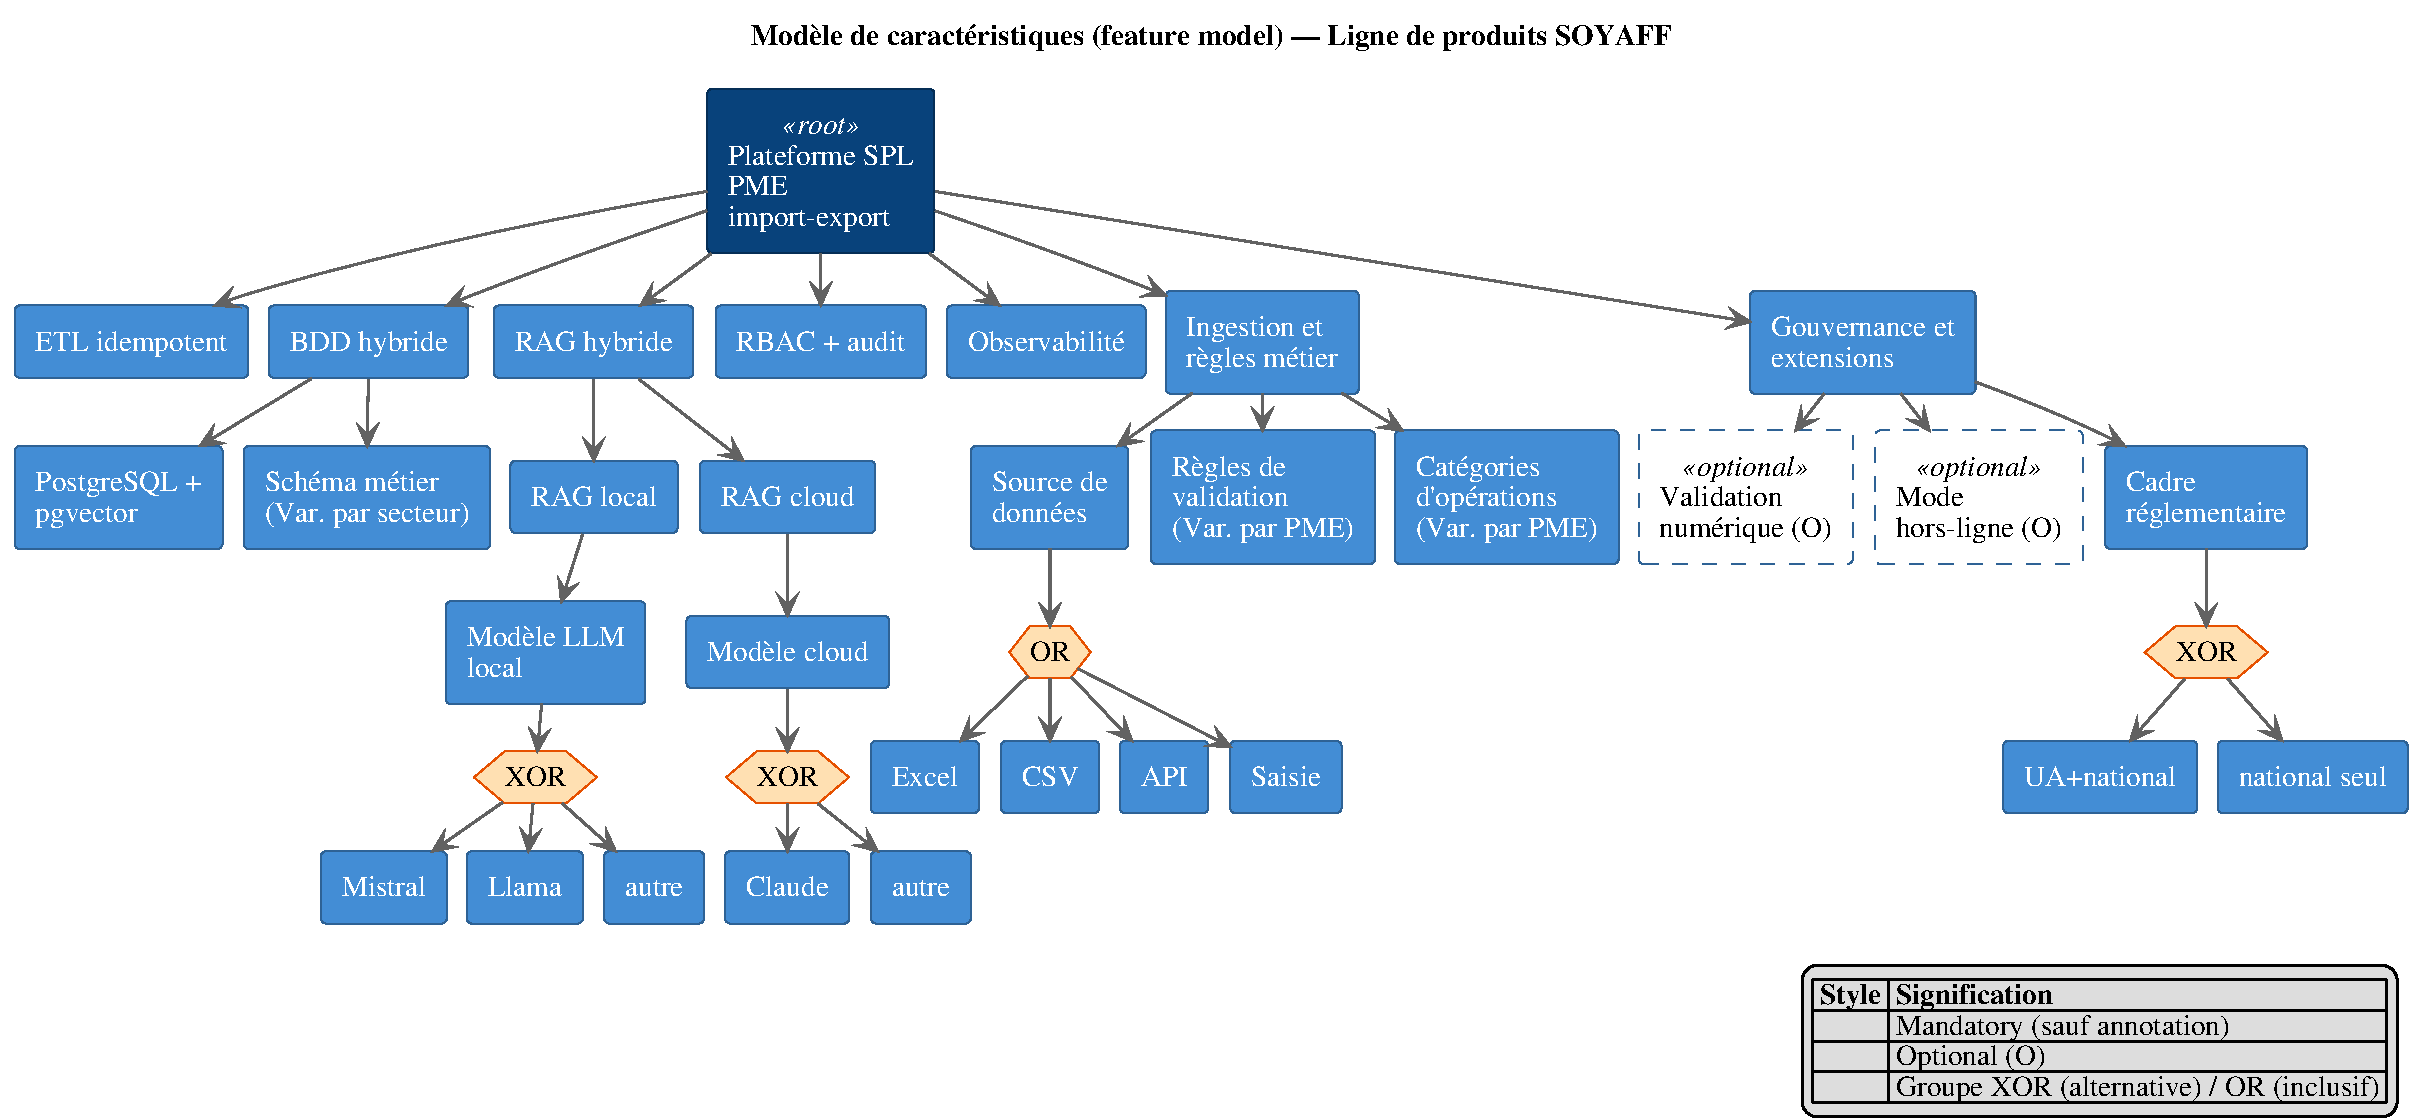
\includegraphics[width=\linewidth,height=0.85\textheight,keepaspectratio]{figures/fig_feature_model.pdf}
    \caption[Modèle de caractéristiques de la ligne de produits SOYAFF]{Modèle de caractéristiques (\textit{feature model}) de la ligne de produits SOYAFF. Sauf annotation contraire, une caractéristique est obligatoire.}
    \label{fig:feature_model_spl}
    \source{Schéma de l'auteur}
\end{figure}
\end{landscape}

Toutes les branches de premier niveau sont obligatoires. Trois d'entre elles (ETL idempotent, RBAC et audit, supervision) n'ont aucune variabilité. Les autres ne varient que dans leurs feuilles, jamais dans leur existence. C'est l'argument central pour H4 : la réutilisation est forte, et la variabilité est bornée à quelques points identifiés. Une contrainte n'apparaît pas dans l'arbre : le RAG local \emph{requiert} un moteur d'inférence local, donc le conteneur Ollama.

\subsection{Instanciation illustrative : SODRAF SARL (Bamako, Mali)}
\label{sec:spl_instanciation}

Pour rendre l'analyse concrète, nous dérivons sur le papier un second produit pour SODRAF SARL. Cette société de commerce d'import-export de produits alimentaires (riz, sucre, boissons), basée à Bamako, emploie de 51 à 200 personnes et est \textbf{partenaire commercial de SOYAFF} sur le corridor. Il s'agit d'une dérivation analytique, pas d'un déploiement.

\textbf{Ce qui est repris tel quel.} SODRAF gère elle aussi ses opérations sur des supports hétérogènes. Les six invariants sont repris sans modification : mêmes conteneurs, même topologie, même routage hybride.

\textbf{Ce qui est reconfiguré.}
\begin{itemize}
    \item \textbf{Le schéma métier.} Les camions, bons de livraison et chauffeurs laissent la place aux fournisseurs, produits, stocks et points de vente. C'est une modélisation de domaine à part entière, pas un paramétrage.
    \item \textbf{Le cadre juridique.} SODRAF relève du régime malien, hors Convention de Malabo : le socle juridique change de nature.
    \item \textbf{Les catégories et les règles métier.} Les catégories du transport (carburant, ration, frais de route) deviennent celles du commerce (achat, stockage, distribution, pertes) ; les contrôles de délai sont remplacés par des seuils de réapprovisionnement ou de péremption.
\end{itemize}

Aucun conteneur du plan applicatif, IA ou données (Tableau~\ref{tab:inventaire_conteneurs}) n'est remplacé ni supprimé. La charge réelle de reconfiguration du schéma n'a cependant pas été mesurée, et rien ne garantit qu'elle resterait contenue en pratique.

\subsection{Portée, limites et verdict sur H4}
\label{sec:spl_limites}

\textbf{Verdict.} L'architecture présente un noyau de six invariants et une variabilité bornée à sept points identifiés ; la dérivation vers SODRAF ne modifie aucun conteneur. \textbf{H4 est étayée analytiquement} : la réplicabilité est plausible sans refonte majeure. Elle n'est ni validée ni infirmée par l'expérience.

\textbf{Limites.}
\begin{itemize}
    \item \textbf{Un seul produit réel.} SOYAFF est le seul membre de la ligne construit et exploité ; SODRAF n'est dérivée que sur le papier.
    \item \textbf{Une variabilité en partie théorique.} Le modèle local est écrit en dur dans le code : le changer demande une modification du code, pas une simple configuration.
    \item \textbf{Le schéma métier reste le point le plus large.} Changer de secteur, même vers un secteur voisin, demande une nouvelle modélisation du domaine.
    \item \textbf{Le cadre juridique change de nature d'un pays à l'autre}, ce qui nuance l'idée d'une variabilité uniformément bornée.
\end{itemize}

La validation par un déploiement réel, chez SODRAF de préférence, est la suite logique de ce travail (section~\ref{chap:perspectives}).

\subsection{Synthèse et transition}
\label{sec:spl_synthese_transition}

H4 est étayée par l'analyse, pas encore démontrée par un second cas. Les quatre hypothèses ont maintenant été éprouvées : H2 par le benchmark, H1 et H3 par la mesure de l'impact, H4 par le raisonnement. Il reste à chiffrer le retour sur investissement (\S\ref{sec:roi}) et à répondre à la problématique (\S\ref{sec:reponse_problematique}).


\section{Retour sur investissement}
\label{sec:roi}

Cette section chiffre ce que la plateforme rapporte à SOYAFF, en FCFA. Nous ne valorisons pas des suppressions de postes : aucun emploi n'est supprimé. Le gain est du temps de travail libéré, valorisé au coût de la personne qui le récupère. Nous distinguons ce qui a été mesuré de ce qui est déclaré.

\subsection{Coûts}
\label{sec:roi_couts}

\textbf{Investissement initial.} Nous avons proposé à SOYAFF de facturer le développement de la plateforme 2~000~000~FCFA. Cette proposition n'est pas encore conclue ; nous la retenons comme valeur de l'investissement, celle qu'une entreprise paierait pour un projet équivalent.

\textbf{Coûts de fonctionnement.} Le Tableau~\ref{tab:roi_couts} détaille les dépenses mensuelles, converties au taux du 27~septembre~2026 (1~USD~=~598,02~FCFA).

\begin{table}[H]
\centering
\footnotesize
\caption{Coûts mensuels de fonctionnement de la plateforme}
\label{tab:roi_couts}
\begin{tabularx}{\linewidth}{|>{\raggedright\arraybackslash}X|r|r|}
\hline
\rowcolor[HTML]{EFEFEF}
\textbf{Poste} & \textbf{Montant facturé} & \textbf{Coût mensuel (FCFA)} \\ \hline
Serveur dédié OneProvider (sauvegarde de 100~Go incluse) & 30,23~USD par mois & 18~078 \\ \hline
API Anthropic (chemin cloud) & $\approx$~10~USD par mois & 5~980 \\ \hline
Nom de domaine & 10~USD par an & 498 \\ \hline
Logiciels (PostgreSQL, Airflow, n8n, Grafana, Docker\ldots) & 0 & 0 \\ \hline
\textbf{Total mensuel} & \textbf{41,06~USD} & \textbf{24~557} \\ \hline
\textbf{Total annuel} & & \textbf{294~680} \\ \hline
\end{tabularx}
\end{table}

\subsection{Gains}
\label{sec:roi_gains}

\textbf{Gain mesuré : la saisie à Dakar.} Le chronométrage du §\ref{sec:impact_temps} établit qu'une opération prend 11,16~minutes dans Excel et 1,71~minute sur la plateforme, soit 9,45~minutes gagnées. La base de production compte 4~756 transactions sur seize mois, soit environ 297 opérations par mois. L'agent de saisie récupère donc près de 47~heures par mois. Payé 400~000 à 500~000~FCFA par mois pour 173~heures de travail, son heure coûte 2~308 à 2~885~FCFA. Le temps libéré vaut ainsi \textbf{108~000 à 135~000~FCFA par mois}.

\textbf{Gain déclaré : la fin de la double saisie à Bamako.} Le chef logistique ne ressaisit plus les récapitulatifs envoyés de Dakar. Ce gain n'a pas été chronométré. Le chef logistique l'estime à deux heures par jour : la ressaisie lui prenait, selon ses mots, une bonne partie de la journée. Payé plus de 500~000~FCFA par mois, il récupère environ 43~heures mensuelles, soit au moins \textbf{125~000~FCFA par mois}. Nous présentons ce gain comme une estimation déclarée, non comme une mesure.

\subsection{Retour sur investissement}
\label{sec:roi_calcul}

Le Tableau~\ref{tab:roi_scenarios} présente deux scénarios. Le scénario~A ne retient que le gain mesuré à Dakar : c'est le plancher, que le jury peut vérifier sur les données du §\ref{sec:impact_temps}. Le scénario~B y ajoute le gain déclaré à Bamako.

\begin{table}[H]
\centering
\footnotesize
\caption{Retour sur investissement selon deux scénarios (297 opérations par mois)}
\label{tab:roi_scenarios}
\begin{tabularx}{\linewidth}{|>{\raggedright\arraybackslash}X|r|r|}
\hline
\rowcolor[HTML]{EFEFEF}
\textbf{Indicateur (FCFA)} & \textbf{A : mesuré} & \textbf{B : mesuré + déclaré} \\ \hline
Gain mensuel & 108~000 à 135~000 & 233~000 à 260~000 \\ \hline
Coût mensuel & 24~557 & 24~557 \\ \hline
\textbf{Gain net mensuel} & \textbf{83~000 à 110~000} & \textbf{208~000 à 235~000} \\ \hline
\textbf{Amortissement de 2~000~000~FCFA} & \textbf{18 à 24 mois} & \textbf{8,5 à 9,6 mois} \\ \hline
\end{tabularx}
\end{table}

Dans les deux scénarios, la plateforme rapporte plus qu'elle ne coûte dès le premier mois d'exploitation : le gain mensuel représente quatre à dix fois le coût de fonctionnement. Ce qui varie, c'est le délai pour rembourser l'investissement initial : moins de dix mois si l'on compte le gain de Bamako, un an et demi à deux ans sur le seul gain mesuré.

\textbf{Projection sur trois ans.} Le Tableau~\ref{tab:roi_projection} suit les deux scénarios année par année, pour un agent payé 450~000~FCFA (milieu de la fourchette).

\begin{table}[H]
\centering
\footnotesize
\caption{Projection financière sur trois ans (agent à 450~000~FCFA par mois)}
\label{tab:roi_projection}
\begin{tabular}{|l|r|r|r|r|}
\hline
\rowcolor[HTML]{EFEFEF}
\textbf{Année} & \textbf{Investissement} & \textbf{Coûts} & \textbf{Bilan cumulé A} & \textbf{Bilan cumulé B} \\ \hline
Année 1 & 2~000~000 & 294~680 & $-$837~381 & 662~619 \\ \hline
Année 2 & 0 & 294~680 & 325~237 & 3~325~237 \\ \hline
Année 3 & 0 & 294~680 & 1~487~856 & 5~987~856 \\ \hline
\end{tabular}
\end{table}

Sur trois ans, le bilan cumulé atteint environ 1,49~million de FCFA dans le scénario~A et 5,99~millions dans le scénario~B. Le volume d'opérations joue fortement : avec les 438 opérations de mars~2026 au lieu de la moyenne de 297, l'amortissement du scénario~B tombe à 7,2~mois.

\textbf{Ce que ce calcul ne compte pas.} Trois bénéfices ne sont pas valorisés, faute de mesure fiable : la réduction des erreurs de saisie (§\ref{sec:impact_erreurs}), la disponibilité de l'information en temps réel pour les décideurs, et le temps gagné par l'assistant conversationnel sur les analyses. Le retour sur investissement présenté ici est donc un minimum. À l'inverse, il suppose que le temps libéré est réemployé à des tâches utiles ; s'il ne l'est pas, le gain reste réel pour les personnes, mais pas pour la trésorerie.

\section{Réponse à la problématique}
\label{sec:reponse_problematique}

La problématique posée en introduction demandait comment concevoir, déployer et valider une architecture logicielle hybride et réplicable pour digitaliser une PME d'import-export ouest-africaine, sous des contraintes de budget, de connectivité et de souveraineté des données. Le Tableau~\ref{tab:reponse_questions} reprend les quatre questions de recherche qui la déclinent ; les paragraphes qui suivent y répondent une à une.

\begin{table}[H]
\centering
\footnotesize
\caption{Réponse aux questions de recherche}
\label{tab:reponse_questions}
\begin{tabularx}{\linewidth}{|l|>{\raggedright\arraybackslash}X|l|}
\hline
\rowcolor[HTML]{EFEFEF}
\textbf{Question} & \textbf{Réponse établie} & \textbf{Hypothèse} \\ \hline
Q1 : quelle architecture ? & Une plateforme mono-serveur (ETL, application web, IA hybride, DevOps), en production, pour 37,4~€ par mois & H1 confirmée \\ \hline
Q2 : le RAG local vaut-il le cloud ? & Non : 20~\% d'exactitude contre 88,9~\% & H2 réfutée \\ \hline
Q3 : quel impact métier, à quel coût ? & Environ 85~\% de temps de saisie en moins, investissement amorti en 8,5 à 24 mois & H3 confirmée (volet temps) \\ \hline
Q4 : l'architecture se réplique-t-elle ? & Un noyau invariant et des points de variation identifiés, sans second déploiement & H4 étayée analytiquement \\ \hline
\end{tabularx}
\end{table}

\textbf{D'une chaîne de fichiers Excel à une plateforme d'aide à la décision.} Le point de départ était une chaîne de fichiers. L'agent de Dakar saisissait les opérations dans un récapitulatif journalier, les recopiait dans un récapitulatif mensuel, puis envoyait le fichier par WhatsApp. À Bamako, le chef logistique attendait ce fichier, le ressaisissait dans ses propres tableaux, et les deux bureaux s'appelaient longuement pour lever les incohérences. Le point d'arrivée est une plateforme où chaque opération est saisie une seule fois, contrôlée au moment de la saisie et visible aussitôt dans les deux bureaux, avec un assistant qui répond en langage naturel sur l'ensemble des données. C'est la première réponse à la problématique : l'architecture a été conçue et déployée, et elle tourne en production.

\textbf{Q1 et H1 : une architecture frugale et complète.} Un seul serveur dédié porte le pipeline ETL, l'application web, les deux chemins d'IA, l'intégration continue et la supervision, pour 41,06~USD par mois, soit 37,4~€ (§\ref{sec:impact_cout}). Le seuil de 50~€ est respecté avec une marge d'un quart. La contrainte budgétaire n'a donc pas imposé de renoncer à l'une des briques. La contrainte de connectivité, elle, n'est que partiellement traitée : l'application exige une connexion, et le mode hors-ligne reste à construire (§\ref{sec:limites_solution}).

\textbf{Q3 et H3 : un impact mesuré sur le travail quotidien.} Le temps de saisie d'une opération passe de 11,16 à 1,71~minutes, soit une réduction de l'ordre de 85~\% (§\ref{sec:impact_temps}). Les utilisateurs le formulent plus simplement. L'agent de saisie ne saisit plus qu'une fois : fini la copie du journalier vers le mensuel et l'envoi par WhatsApp. Le chef logistique n'attend plus de fichier pour travailler : il voit chaque opération dès qu'elle est saisie. Le score d'utilisabilité de 88,1 (§\ref{sec:adoption_resultats}) et les entretiens confirment cette utilité perçue. En valorisant le temps libéré, l'investissement de 2~000~000~FCFA est amorti en 8,5 à 24 mois selon le scénario retenu (§\ref{sec:roi}).

\textbf{Q2 et H2 : la souveraineté tient, l'exactitude locale non.} Le benchmark a été la principale déception de ce travail. Le RAG local n'atteint que 20~\% d'exactitude, loin des 88,9~\% du cloud (§\ref{sec:bench_resultats_globaux}), et H2 est réfutée. Ce résultat ne remet pas en cause le principe de souveraineté : le routage hybride fonctionne de bout en bout, et les questions sensibles ne quittent pas le serveur (§\ref{sec:test_bout_en_bout}). Ce qu'il remet en cause, c'est la méthode de récupération du chemin local. Chercher par similarité sémantique dans des données relationnelles, pour répondre à des questions d'agrégat, était inadapté : le diagnostic le montre question par question (§\ref{sec:bench_diagnostic}). La réponse n'est pas d'abandonner le chemin local, mais de lui donner la méthode qui réussit côté cloud : générer une requête SQL à partir de la question (\textit{text-to-SQL}), avec un modèle exécuté sur le serveur. C'est la principale perspective de ce travail.

\textbf{Q4 et H4 : une réplicabilité étayée, pas encore démontrée.} L'analyse par lignes de produits logiciels distingue un noyau invariant, valable pour toute PME du même type (le pipeline ETL, l'IA hybride, le déploiement frugal sur un seul serveur), et des points de variation configurables (le schéma de la base, les rôles d'accès, une partie des règles métier) (§\ref{sec:spl_invariants}, §\ref{sec:spl_variation}). La dérivation vers SODRAF, entreprise partenaire de SOYAFF, est restée sur le papier : le temps a manqué pour la déployer. H4 est donc étayée par le raisonnement, pas encore par un second cas réel.

\textbf{En réponse à la problématique.} Une PME d'import-export ouest-africaine peut être digitalisée par une architecture hybride conçue pour ses contraintes : le système existe, il est utilisé, il fait gagner du temps et il coûte moins de 50~€ par mois. L'hybride tient comme principe de souveraineté. Il ne tient pas encore comme promesse d'exactitude sur le chemin local, et le benchmark indique précisément quoi changer pour y parvenir.

\section{Limites de la solution}
\label{sec:limites_solution}

Les résultats de ce chapitre valent dans des limites que nous rassemblons ici. Chacune est détaillée dans la section qui l'a établie ; le chapitre~\ref{chap:discussion_perspectives} en tire les conséquences sans les répéter.

\textbf{Limites techniques.}
\begin{itemize}
    \item \textbf{Le chemin local n'est pas fiable pour l'analyse.} Il atteint 20~\% d'exactitude, et ses réponses SQL directes peuvent être fausses tout en paraissant certaines : une somme à la place d'un comptage, une plaque qui fait ignorer le reste de la question (§\ref{sec:bench_diagnostic}). H2 est réfutée.
    \item \textbf{Le classifieur de sensibilité reste lexical.} Un nom de chauffeur cité seul, sans le mot « chauffeur » ni plaque, n'est pas détecté et part vers le cloud. Le rôle en lecture seule de l'agent, qui n'a pas accès à la table \texttt{chauffeurs}, borne ce risque sans le supprimer (§\ref{sec:ia_routage}). La précision du classifieur n'a pas été mesurée.
    \item \textbf{Un seul serveur.} Une panne arrête tous les services ; le déploiement n'a pas de retour arrière automatique (§\ref{sec:devops_dettes}).
    \item \textbf{Deux exigences restent à construire} : le mode hors-ligne (\texttt{ENF-DISP-01}), alors que la connectivité est une contrainte du terrain, et le circuit de validation numérique (\texttt{EF-VAL-02}) (§\ref{sec:webapp_fonctionnalites_cibles_non_deployees}).
\end{itemize}

\textbf{Limites de la mesure.}
\begin{itemize}
    \item \textbf{Le benchmark a été exécuté sur le serveur lui-même.} Ses latences n'incluent pas le trajet réseau jusqu'au poste de l'utilisateur. Les verdicts ont été attribués par un seul annotateur, sur un corpus rédigé par le concepteur du système (§\ref{sec:bench_limites}).
    \item \textbf{Le gain de temps repose sur cinq sessions rejouées} par un seul agent, avec un effet d'observation possible (§\ref{sec:impact_limites}). Le volet erreurs de H3 n'est que partiellement étayé : le seuil de 80~\% n'a pas pu être vérifié (§\ref{sec:impact_erreurs}).
    \item \textbf{L'adoption porte sur quatre utilisateurs.} C'est un recensement de tous les utilisateurs métier, pas un échantillon : le score SUS de 88,1 décrit ce cas, il ne se généralise pas (§\ref{sec:adoption_biais}).
    \item \textbf{Le gain de Bamako est déclaré, non mesuré}, et le retour sur investissement suppose que le temps libéré est réemployé (§\ref{sec:roi}).
    \item \textbf{La disponibilité est mesurable mais n'a pas été mesurée} sur une période significative (§\ref{sec:impact_cout}).
\end{itemize}

\textbf{Limites de contexte.}
\begin{itemize}
    \item \textbf{Un seul cas.} Toutes les mesures portent sur SOYAFF. H4 est étayée par un raisonnement sur les lignes de produits logiciels et une dérivation sur le papier vers une seconde PME, pas par un second déploiement (§\ref{sec:spl_limites}).
    \item \textbf{Des coûts en dollars.} Le serveur et l'API sont facturés en USD, alors que le franc CFA est arrimé à l'euro : le coût mensuel varie avec le taux de change.
    \item \textbf{Des données personnelles hors du serveur.} La copie de sauvegarde hors site n'est pas encore chiffrée (§\ref{sec:devops_dettes}), et les questions non sensibles, avec les résultats de l'agent, sont traitées par un service tiers.
\end{itemize}

\chapter{Discussion et perspectives}
\label{chap:discussion_perspectives}

Ce dernier chapitre prend du recul sur les résultats du chapitre~\ref{chap:evaluation}. Il en discute le sens et la validité (section~\ref{chap:discussion}), puis trace les évolutions de la plateforme (section~\ref{chap:perspectives}).

\section{Discussion des résultats}
\label{chap:discussion}

Cette section ne produit aucune mesure nouvelle. Elle croise les résultats du chapitre~\ref{chap:evaluation} pour dire ce qu'ils signifient ensemble, prend position sur le sens de la contribution après la réfutation de H2, revient sur le risque de sécurité découvert pendant la réalisation, puis examine la validité de l'ensemble. Les limites propres à chaque mesure ne sont pas répétées : elles sont rassemblées au §\ref{sec:limites_solution}.

\subsection{Bilan croisé des quatre hypothèses}
\label{sec:disc_bilan}

\textbf{Le récit d'ensemble.} Prises une à une, les hypothèses donnent chacune un verdict. La plateforme est frugale : 37,4~€ par mois, sous le seuil de 50~€ avec une marge d'un quart (H1, §\ref{sec:impact_cout}). Elle transforme le travail quotidien : environ 85~\% de temps de saisie en moins (H3, §\ref{sec:impact_temps}). Elle est adoptée par tous ses utilisateurs, avec un score SUS moyen de 88,1 (§\ref{sec:adoption_resultats}). Son architecture est réplicable en théorie (H4, §\ref{sec:spl_limites}). Prises ensemble, elles racontent une histoire plus précise : la plateforme réussit sur presque tous les plans, \emph{sauf} sur celui qui portait sa promesse la plus originale. Le RAG local n'atteint que 20~\% d'exactitude contre 88,9~\% pour le cloud (H2, §\ref{sec:bench_resultats_globaux}). C'est cette tension qui fait la matière de cette discussion.

\textbf{Les résultats s'éclairent mutuellement.} Le faible coût du chemin cloud, 0,033~USD par question (§\ref{sec:bench_resultats_globaux}), amortit l'échec de H2 : la marge de H1 permet d'envoyer environ 400 questions de plus par mois vers le cloud avant d'atteindre le seuil. Ensuite, le seul volet de H2 qui survit à la réfutation, la souveraineté du chemin local, devient la seule raison de conserver ce chemin : sans elle, rien ne justifierait un service aussi en retrait. Enfin, l'adoption mesurée porte surtout sur le chemin cloud, qui répond à l'essentiel des questions analytiques : elle valide la plateforme telle qu'elle est utilisée, pas l'ambition initiale d'un RAG local à parité. Les hypothèses forment ainsi un système, où la solidité des unes compense la fragilité de l'autre.

\subsection{Le sens de la contribution : la thèse hybride à l'épreuve}
\label{sec:disc_sens}

\textbf{Ce que « hybride » signifiait, et ce que les résultats en font.} L'introduction présentait l'hybride cloud/local comme le meilleur des deux mondes : la souveraineté du local et la puissance du cloud, arbitrées selon la sensibilité de chaque question. Le benchmark oblige à reformuler cette promesse. Sur des questions structurées et quantitatives, qui forment l'essentiel des besoins de SOYAFF, le chemin local ne rivalise pas. L'hybride tient, mais comme un arbitrage explicite entre souveraineté et exactitude, et non comme deux chemins équivalents. La thèse est plus étroite que celle de départ ; elle est aussi plus juste.

\textbf{Ce que l'échec de H2 enseigne.} Le diagnostic du §\ref{sec:bench_diagnostic} montre que l'échec ne vient pas d'abord du modèle. Il vient de la façon de récupérer les données. Les règles SQL du chemin local sont rapides mais mal ciblées : elles renvoient une somme quand on demande un nombre, ou ignorent le mot-clé quand une plaque est citée. La recherche par similarité sémantique, elle, ne peut pas produire un \texttt{COUNT} ou un \texttt{SUM} exact sur une base relationnelle, quel que soit le modèle qui exploite ensuite le résultat. L'agent cloud réussit parce qu'il écrit lui-même sa requête SQL sur toute la base. Ce diagnostic est en lui-même une contribution : il sera plus utile au concepteur d'un système similaire qu'une parité confirmée.

\textbf{La conséquence de conception.} Si l'écart tient à la récupération et non au modèle, un meilleur \textit{prompt} ou un modèle local plus gros n'y changeront rien. Il faut donner au chemin local la méthode qui réussit côté cloud : traduire la question en requête SQL (\textit{text-to-SQL}), avec un modèle exécuté sur le serveur et un accès en lecture seule. C'est la principale perspective de ce travail (§\ref{sec:persp_moyen}). Le benchmark l'a révélée en échouant.

\textbf{Ce que ce travail démontre malgré H2.} La réfutation de H2 ne doit pas masquer le reste. Une PME d'import-export ouest-africaine peut exploiter, pour 37,4~€ par mois, une plateforme qui supprime une double saisie coûteuse (chapitre~\ref{chap:contexte}, §\ref{sec:diagnostic_si}), qui est adoptée par tous ses utilisateurs et qui garde sur le serveur les questions sensibles. Ce résultat ne dépend pas de H2 : il tient même si le chemin local reste durablement en retrait.

\subsection{Un risque de sécurité identifié, puis corrigé}
\label{sec:disc_risque}

\textbf{Le risque composé.} Pendant la réalisation, nous avions relevé deux écarts du module IA qui, combinés, formaient un risque plus grave que chacun pris seul. D'une part, le classifieur de sensibilité envoyait au cloud une question d'agrégat même quand elle nommait un chauffeur ou un camion (« le total des rations du chauffeur du camion AA~085~AH »). D'autre part, l'outil SQL de l'agent cloud n'avait aucune contrainte technique : seule la consigne du \textit{system prompt} limitait ce qu'il pouvait exécuter. Ensemble, ces deux écarts permettaient qu'une question sensible mal classée fasse exécuter, côté cloud, une requête non contrainte sur la base, dont le résultat sortait de l'infrastructure.

\textbf{La correction.} Nous avons traité les deux causes avant la mesure finale. L'identité l'emporte désormais sur l'agrégat : toute mention d'un chauffeur ou d'une plaque reste locale (§\ref{sec:ia_routage}). L'agent cloud se connecte avec un rôle PostgreSQL en lecture seule, sans accès aux données des chauffeurs (§\ref{sec:ia_cloud}). Le test du §\ref{sec:test_refus} le montre : une demande de suppression est refusée, et la base la rejetterait même si le modèle la générait. Le risque n'est pas nul pour autant : un nom de chauffeur cité seul échappe encore au classifieur. Mais la base empêche l'agent de le relier à des données personnelles.

\textbf{La portée exacte de la souveraineté.} Ce qui est garanti par construction, c'est que le chemin local ne fait sortir aucune donnée du serveur. Le chemin cloud, lui, traite par nature des données chez un tiers, limitées aux questions non sensibles et aux tables métier. La formulation juste est donc que la souveraineté est garantie sur le chemin local et bornée sur le chemin cloud, pas qu'elle vaut globalement pour tout le système.

\subsection{Limites transversales de la démarche}
\label{sec:disc_limites}

Deux limites dépassent une mesure particulière et bornent l'ensemble du travail.

\textbf{Le chercheur intégré.} L'auteur est à la fois le concepteur de la plateforme, son administrateur, un collègue des utilisateurs interrogés et l'unique annotateur du benchmark. Cette position touche plusieurs résultats : un biais de complaisance possible dans l'étude SUS (§\ref{sec:adoption_biais}), atténué par la dispersion des scores et la précision des critiques recueillies, et une annotation non croisée du benchmark (§\ref{sec:bench_limites}). Elle appelle une lecture prudente de tout résultat qui repose sur un jugement humain plutôt que sur une référence objective.

\textbf{Des mesures prises sur deux états du système.} Le chronométrage et l'étude d'adoption ont été conduits en juillet~2026 (le questionnaire SUS le 22~juillet). Le benchmark et le test de bout en bout l'ont été le 27~septembre, après des évolutions du code : contrôle des délais de saisie, correction du classifieur, rôle en lecture seule, calcul SQL des totaux. Les chiffres de temps et d'adoption décrivent donc la version de juillet. Le contrôle des délais ajoute une vérification à la saisie ; son effet sur le temps de saisie et sur la satisfaction des utilisateurs n'a pas été mesuré.

\subsection{Menaces à la validité}
\label{sec:disc_validite}

Nous reprenons ici, selon le cadre classique des quatre types de validité, des réserves posées au fil du chapitre~\ref{chap:evaluation}.

\textbf{Validité de construit : les mesures mesurent-elles ce qu'elles prétendent ?} Le temps « avant » n'est pas celui d'une saisie Excel d'époque, mais celui d'une ressaisie rejouée par un agent qui ne pratique plus Excel au quotidien (§\ref{sec:impact_limites}). Le questionnaire SUS est une traduction française non revalidée : rien ne garantit qu'il mesure l'utilisabilité exactement comme l'instrument original \cite{brookeSUSAQuickDirty1996}.

\textbf{Validité interne : les conclusions causales tiennent-elles ?} Le gain de temps pourrait devoir une part à l'apprentissage et au rejeu. Mais la marge de quinze points au-dessus du seuil de H3 absorbe toute correction plausible de ce biais (§\ref{sec:impact_limites}).

\textbf{Validité externe : les résultats se généralisent-ils ?} Un seul cas, quatre utilisateurs et un corpus propre au transport Dakar--Bamako interdisent toute généralisation statistique. H4, étayée par un raisonnement plutôt que par une réplication (§\ref{sec:spl_limites}), est la seule réponse, partielle, à cette limite.

\textbf{Validité de conclusion : les chiffres soutiennent-ils les verdicts ?} Le verdict sur H2 repose sur 180 réponses, trois passages par question et une référence SQL calculée le jour de la mesure : l'écart entre 20~\% et 88,9~\% est trop large pour qu'une erreur d'annotation l'inverse. Le seuil de 80~\% de réduction des erreurs de H3, à l'inverse, n'a pas pu être vérifié : l'échantillon était trop propre pour qu'un ratio soit calculable, et le verdict a été requalifié plutôt que forcé (§\ref{sec:impact_erreurs}).

\subsection{Synthèse et transition}
\label{sec:disc_synthese}

Ce que ce travail établit solidement ne dépend pas de H2 : une plateforme frugale, qui supprime une double saisie mesurée, adoptée par tous ses utilisateurs et réplicable en théorie. Ce qu'il nuance est assumé : l'hybride tient comme arbitrage entre souveraineté et exactitude, et l'échec du chemin local désigne précisément la méthode à changer. Ce qu'il ne peut pas conclure est nommé : la réplicabilité au-delà d'un cas, la disponibilité réelle, le seuil de réduction des erreurs. Ces questions ouvertes tracent un programme de travail, objet de la section suivante.

\section{Perspectives}
\label{chap:perspectives}

Cette section transforme les résultats et les limites de ce travail en programme de travail. Chaque piste part d'un résultat mesuré, d'une dette nommée ou d'une demande des utilisateurs. Nous les organisons en trois horizons : consolider (§\ref{sec:persp_court}), corriger et étendre (§\ref{sec:persp_moyen}), valider et changer d'échelle (§\ref{sec:persp_long}).

\subsection{Court terme : consolider}
\label{sec:persp_court}

Les pistes de court terme se traitent par de la mesure, de la configuration ou un développement limité, sans remettre en cause l'architecture. Le Tableau~\ref{tab:persp_court} les résume.

\begin{table}[htbp]
\centering
\footnotesize
\caption{Pistes à court terme}
\label{tab:persp_court}
\begin{tabular}{|>{\raggedright\arraybackslash}p{5.0cm}|>{\raggedright\arraybackslash}p{2.8cm}|>{\raggedright\arraybackslash}p{2.4cm}|>{\raggedright\arraybackslash}p{2.0cm}|}
\hline
\rowcolor[HTML]{EFEFEF}
\textbf{Piste} & \textbf{Origine} & \textbf{Effort} & \textbf{Priorité} \\ \hline
Corriger les règles SQL du chemin local, puis rejouer le benchmark & §\ref{sec:bench_dettes} & Petit développement & \textbf{1} \\ \hline
Chiffrer la copie de sauvegarde hors site (\texttt{rclone crypt}) & §\ref{sec:devops_dettes} & Configuration & \textbf{1} \\ \hline
Mesurer la disponibilité (\texttt{ENF-DISP-02}) sur les sondes existantes & §\ref{sec:impact_cout} & Mesure & 2 \\ \hline
Mesurer la précision du classifieur de sensibilité & §\ref{sec:ia_routage} & Mesure & 2 \\ \hline
Faire annoter le benchmark par un second évaluateur & §\ref{sec:bench_limites} & Mesure & 2 \\ \hline
Mesurer la couverture des tests Node en CI & §\ref{sec:devops_dettes} & Configuration & 3 \\ \hline
Versionner la configuration Nginx du serveur & §\ref{sec:devops_dettes} & Configuration & 3 \\ \hline
Prévoir un retour arrière automatique au déploiement & §\ref{sec:devops_dettes} & Petit développement & 3 \\ \hline
Abstraire l'interface d'inférence locale (\texttt{ENF-MAINT-01}) & §\ref{sec:ia_dettes} & Petit développement & 3 \\ \hline
\end{tabular}
\end{table}

\textbf{Corriger ce que le benchmark a révélé.} La piste la plus rentable est aussi la plus simple. Seize questions sur trente passent déjà par le calcul SQL du chemin local, et onze de ces réponses sont fausses pour trois raisons identifiées (§\ref{sec:bench_diagnostic}) : distinguer une question de comptage d'une question de somme, combiner le filtre sur la plaque avec le mot-clé, filtrer sur la catégorie de l'opération plutôt que sur les libellés. Ces corrections ne touchent pas au modèle de langage. Le benchmark, rejoué dans les mêmes conditions, dira ce qu'elles valent.

\textbf{Protéger et mesurer.} La sauvegarde est en place, mais sa copie hors site, qui contient des données personnelles, n'est pas chiffrée : le script prévoit déjà le chiffrement côté client, il reste à l'activer. La disponibilité, la précision du classifieur et l'accord entre deux annotateurs du benchmark sont des mesures sans développement : l'instrumentation et les données existent.

\subsection{Moyen terme : corriger l'architecture et étendre les fonctions}
\label{sec:persp_moyen}

\textbf{Un \textit{text-to-SQL} local : la perspective phare.} Le benchmark a montré qu'une recherche par similarité sémantique était inadaptée à des données relationnelles interrogées par agrégats (§\ref{sec:disc_sens}). L'agent cloud réussit parce qu'il traduit la question en requête SQL et l'exécute sur toute la base. Nous proposons de donner cette capacité au chemin local : un modèle exécuté sur le serveur génère la requête SQL, qui s'exécute avec un rôle en lecture seule, comme celui de l'agent cloud. Les règles SQL corrigées à court terme resteraient en première ligne pour les questions simples ; le \textit{text-to-SQL} prendrait le relais pour les autres. C'est un développement réel, pas un correctif : il touche le cœur du service local, exige un modèle capable de produire du SQL correct sur processeur, et appelle une nouvelle campagne de mesure. Il ne cherche pas à contourner la réfutation de H2 : il la remettrait en jeu, dans une architecture corrigée.

\textbf{Des fonctions réclamées par les utilisateurs.} Les entretiens (§\ref{sec:adoption_qualitatif}) ont fait remonter des demandes qui recoupent des exigences déjà spécifiées : le circuit de validation numérique (\texttt{EF-VAL-02}), réclamé par le chef de bureau pour valider les dépenses avant leur enregistrement ; le mode hors-ligne (\texttt{ENF-DISP-01}), réclamé par l'agent de saisie pour ne plus dépendre du réseau ; une alerte de seuil de caisse, extension du suivi de caisse (\texttt{EF-DSH-01}) ; un filtre avancé pour les camions particuliers (\texttt{EF-DSH-03}, \texttt{EF-DSH-04}), réclamé par le chef logistique. Le mode hors-ligne mérite une attention particulière : la connectivité est une contrainte du terrain posée dès la problématique.

\textbf{Un choix de périmètre : \texttt{EF-DSH-05}.} Le signalement automatique des dépenses anormales (dérive de coût par camion, montant aberrant) a été spécifié dès l'analyse des besoins, classé \textit{Could have} et renvoyé aux perspectives. Ce n'est pas un manque réclamé à l'usage, mais une extension naturelle une fois les données consolidées.

\subsection{Long terme : valider et changer d'échelle}
\label{sec:persp_long}

\textbf{Un second déploiement, chez SODRAF.} L'analyse par lignes de produits logiciels a étayé H4 sur le papier (§\ref{sec:spl_instanciation}). Le temps a manqué pour aller plus loin. La suite logique est de déployer réellement la plateforme chez SODRAF SARL, entreprise partenaire de SOYAFF à Bamako. Ce déploiement mesurerait ce que l'analyse ne peut pas établir : la charge réelle de reconfiguration du schéma de la base, le point de variation le plus large (§\ref{sec:spl_variation}). C'est un projet à part entière, avec son recueil de besoins, sa migration de données et son accompagnement au changement.

\textbf{Vers une plateforme SaaS multi-tenant.} La plateforme actuelle sert une seule entreprise. Une version mutualisée servirait plusieurs PME, en isolant strictement les données de chacune. L'analyse SPL en donne le plan : le noyau invariant (\S\ref{sec:spl_invariants}) deviendrait le socle commun, et les points de variation (\S\ref{sec:spl_variation}) les paramètres de chaque client. Cette trajectoire implique cependant une refonte : isolation des données par schéma ou par base, cloisonnement des embeddings, modèle d'accès intégrant la notion de client (le RBAC actuel à trois rôles ne la prévoit pas) et modèle économique à définir.

\subsection{Synthèse}
\label{sec:persp_synthese}

Ce programme suit trois temps : consolider ce qui est construit mais pas encore assez mesuré ou protégé, corriger le chemin local et étendre les fonctions demandées par les utilisateurs, puis valider l'architecture sur un second cas avant de la mutualiser. Chaque étape part de ce que ce travail a mesuré ou recueilli. La conclusion referme le mémoire, du diagnostic initial à ce programme.



% ===== CONCLUSION =====
% --- CONCLUSION (sans numérotation) ---
\chapter*{Conclusion}
\addcontentsline{toc}{chapter}{Conclusion}
\label{chap:conclusion}

Ce travail est parti d'un objectif modeste : concevoir un assistant IA. Le choix du cas s'est porté sur SOYAFF, l'entreprise où je travaille comme informaticien. À mesure que le projet avançait, un problème plus profond est apparu. Les chefs de Bamako devaient décider sur des opérations menées à Dakar sans aucune visibilité en temps réel. Ils recevaient des fichiers Excel de plus d'une cinquantaine d'opérations, où l'information se noyait, et les incompréhensions se réglaient par de longs appels téléphoniques entre les deux bureaux. L'assistant est devenu une plateforme complète. Le chef logistique a donné son accord pour la construire, en posant ses conditions : la sécurité, la souveraineté des données. Presque toutes ont été traitées entre le développement et la mise en production.

\textbf{Ce que la plateforme a changé.} Une opération est désormais saisie une seule fois à Dakar et visible aussitôt à Bamako. Le temps de saisie a baissé d'environ 85~\%. Les utilisateurs ont attribué à la plateforme un score d'utilisabilité moyen de 88,1 sur 100. C'est le résultat dont je suis le plus fier : savoir que ce travail facilite le quotidien de mes collègues. Le tout fonctionne sur un seul serveur pour 37,4~€ par mois. Ce chiffre traduit un choix de conception : une PME ouest-africaine a un budget limité et n'est pas prête à payer lourdement pour sa digitalisation, quitte à rester sur Excel. L'architecture a été pensée pour cette réalité. En valorisant le temps libéré, l'investissement initial est amorti en moins de deux ans, et en moins d'un an si l'on compte la fin de la double saisie à Bamako.

\textbf{Ce que le benchmark m'a appris.} Le RAG local n'a répondu juste qu'à 20~\% des questions, contre 88,9~\% pour le cloud. Ce résultat a été une vraie déception. J'ai d'abord cru que le modèle Mistral~7B était en cause. En reprenant les réponses une à une, j'ai compris que je comparais deux méthodes de récupération différentes. L'agent cloud écrit une requête SQL sur toute la base ; le chemin local cherche des passages par similarité sémantique. Or cette recherche est, par construction, inadaptée à des données relationnelles et à des questions d'agrégat : aucun modèle ne peut calculer un total juste à partir de dix lignes approchantes. C'est la principale leçon d'ingénieur de ce travail. Elle vaut au-delà de SOYAFF : avant de comparer deux modèles, il faut s'assurer qu'ils reçoivent les données de la même façon.

\textbf{Ce qui reste à faire.} La suite logique est de doter le chemin local d'un agent \textit{text-to-SQL} exécuté sur le serveur, avec un modèle spécialisé dans la génération de requêtes, comme SQLCoder de Defog, Code Llama ou DeepSeek-Coder. Le chemin souverain disposerait alors de la méthode qui réussit côté cloud, et le benchmark pourrait être rejoué pour retester H2. La réplicabilité reste elle aussi à démontrer sur un second cas réel : l'analyse par lignes de produits logiciels a identifié ce qui se garde et ce qui se reconfigure, mais le déploiement chez SODRAF, entreprise partenaire de SOYAFF, n'a pas pu être mené faute de temps. Après la soutenance, une réunion à Bamako doit décider de la suite du projet avec la direction de SOYAFF.

La digitalisation des PME ouest-africaines reste un défi. Il revient à ses ingénieurs de le relever, pour garder la maîtrise de nos données et rendre nos entreprises plus productives. C'est notre façon de contribuer au développement de l'Afrique. Ce travail montre qu'on peut commencer avec un seul serveur, des outils libres et des utilisateurs qui disent franchement ce qui leur manque.

\clearpage

% ===== BIBLIOGRAPHIE ET ANNEXES (reprise de la numérotation romaine, là où =====
% ===== les pièces liminaires s'étaient arrêtées) =====
\pagenumbering{roman}
\setcounter{page}{\value{derniere_page_romaine}}

% ===== BIBLIOGRAPHIE =====
\defbibnote{datesconsultation}{Les dates de consultation (« visité le ») indiquées pour les ressources en ligne sont les dates où j'ai saisi les références dans Zotero, pendant une phase de mise au propre de la bibliographie. Elles ne correspondent pas aux dates de lecture.\par\medskip}
\printbibliography[heading=bibintoc, title={Références bibliographiques}, prenote=datesconsultation]

% ===== ANNEXES =====
% --- ANNEXES ---
\appendix
\part*{Annexes}
\addcontentsline{toc}{part}{Annexes}

\chapter{Corpus du benchmark RAG et vérité-terrain}
\label{annexe:corpus}

Cette annexe rassemble le corpus complet des 30 questions métier du benchmark comparatif RAG cloud/local (section~\ref{chap:benchmark_rag}, §\ref{sec:bench_protocole}) sa vérité-terrain et le verdict attribué à chaque réponse, à des fins de reproductibilité. Le corpus et les résultats bruts sont versionnés dans le dépôt \texttt{assistant-soyaff-1} (\texttt{benchmark/questions.csv} ; \texttt{benchmark/resultats/vps\_20260927\_2143/}, qui contient les réponses brutes, la vérité-terrain recalculée sur la base de production et l'état du système avant et après la mesure). Ces fichiers font foi en cas d'écart avec les tableaux qui suivent.

\section{Les 30 questions, par catégorie et type de vérité-terrain}

\begin{longtable}{|>{\raggedright\arraybackslash}p{0.9cm}|>{\raggedright\arraybackslash}p{2.7cm}|>{\raggedright\arraybackslash}p{0.9cm}|>{\raggedright\arraybackslash}p{9.2cm}|}
\caption{Corpus des 30 questions métier du benchmark}
\label{tab:annexe_corpus} \\
\hline
\rowcolor[HTML]{EFEFEF}
\textbf{ID} & \textbf{Catégorie} & \textbf{Type} & \textbf{Question} \\ \hline
\endfirsthead
\multicolumn{4}{c}{\tablename\ \thetable\ (suite)} \\ \hline
\rowcolor[HTML]{EFEFEF}
\textbf{ID} & \textbf{Catégorie} & \textbf{Type} & \textbf{Question} \\ \hline
\endhead
Q01 & suivi de flotte & T1 & Combien de camions de type « particulier » ont eu au moins une transaction enregistrée en mars 2026 ? \\ \hline
Q02 & suivi de flotte & T1 & Combien de camions sont actuellement enregistrés avec le statut « actif » dans le système ? \\ \hline
Q03 & suivi de flotte & T2 & Quels camions sont actuellement en statut « maintenance » ? \\ \hline
Q04 & suivi de flotte & T1 & Combien de camions immatriculés au Mali sont des camions de la société (hors particuliers) ? \\ \hline
Q05 & suivi de flotte & T2 & Quels camions n'ont jamais eu de transaction enregistrée depuis leur création ? \\ \hline
Q06 & suivi de flotte & T3 & Comment se répartit la flotte entre camions société et camions particuliers selon le pays d'immatriculation, et que révèle cette répartition sur la structure logistique de SOYAFF ? \\ \hline
Q07 & gestion financière & T1 & Quel est le total des dépenses de carburant du camion CA~0043~MD, toutes périodes confondues ? \\ \hline
Q08 & gestion financière & T1 & Quel est le montant total des amendes enregistrées en mars 2026, tous camions confondus ? \\ \hline
Q09 & gestion financière & T2 & Quels sont les trois camions ayant le plus dépensé en maintenance sur toute la période ? \\ \hline
Q10 & gestion financière & T1 & Quel est le montant total des avances transport versées en mai 2025 ? \\ \hline
Q11 & gestion financière & T2 & Quelles catégories de dépenses dépassent 40 millions de FCFA cumulés sur toute la période ? \\ \hline
Q12 & gestion financière & T3 & Comment la structure des dépenses par catégorie a-t-elle évolué, et quelles catégories pèsent le plus sur la trésorerie de SOYAFF ? \\ \hline
Q13 & analyse des incidents & T1 & Combien d'amendes ont été enregistrées au total depuis le début du suivi (juin 2024) ? \\ \hline
Q14 & analyse des incidents & T2 & Quels camions ont eu au moins une amende en mars 2026 ? \\ \hline
Q15 & analyse des incidents & T1 & Quel est le montant total des amendes payées par le camion CA~6092~MD, toutes périodes confondues ? \\ \hline
Q16 & analyse des incidents & T2 & Quels camions ont enregistré plus de 15 amendes sur toute la période ? \\ \hline
Q17 & analyse des incidents & T1 & Combien de camions distincts ont eu au moins une intervention de maintenance sur la période ? \\ \hline
Q18 & analyse des incidents & T3 & Que révèle la répartition des amendes par camion sur les pratiques de conduite ou les zones à risque du corridor Dakar--Bamako ? \\ \hline
Q19 & conformité documentaire & T1 & Combien de bons de livraison ont été émis en mars 2026 ? \\ \hline
Q20 & conformité documentaire & T2 & Quels bons de livraison n'ont aucun produit associé (bons « orphelins ») ? \\ \hline
Q21 & conformité documentaire & T1 & Combien de bons de livraison ont été émis au total depuis le début du suivi ? \\ \hline
Q22 & conformité documentaire & T1 & Combien de bons de livraison sont actuellement au statut « livré » ? \\ \hline
Q23 & conformité documentaire & T2 & Quels bons de livraison sont associés au camion AA~076~AH ? \\ \hline
Q24 & conformité documentaire & T3 & Le fait que la quasi-totalité des bons de livraison restent au statut « en\_cours » révèle-t-il une lacune dans le processus de clôture documentaire ? Quelles recommandations en tirer ? \\ \hline
Q25 & décision stratégique & T1 & Quel est le montant total des dépenses de ration au premier trimestre 2026 ? \\ \hline
Q26 & décision stratégique & T2 & Quels sont les trois trimestres ayant enregistré les dépenses de ration les plus élevées ? \\ \hline
Q27 & décision stratégique & T1 & Quel est le nombre total de transactions enregistrées en mars 2026 ? \\ \hline
Q28 & décision stratégique & T1 & Quel est le montant total des dépenses de chargement sur l'année 2025 ? \\ \hline
Q29 & décision stratégique & T2 & Quelles catégories de dépenses ont dépassé 100 millions de FCFA cumulés sur toute la période ? \\ \hline
Q30 & décision stratégique & T3 & Au vu des tendances de dépenses en carburant et en maintenance sur les deux dernières années, quelle recommandation stratégique feriez-vous à la direction de SOYAFF pour maîtriser les coûts opérationnels du corridor Dakar--Bamako ? \\ \hline
\end{longtable}

\noindent\footnotesize Nom exact de la catégorie en base (\texttt{categorie} de \texttt{questions.csv}) : \texttt{suivi\_flotte}, \texttt{gestion\_financiere}, \texttt{analyse\_incidents}, \texttt{conformite\_documentaire}, \texttt{decision\_strategique}.
\normalsize

\section{Vérité-terrain des questions T1 et T2}

Pour les 25 questions T1/T2, la réponse de référence est le résultat d'une requête SQL en lecture seule, exécutée sur la base de production le 27~septembre~2026, jour de la mesure. Les requêtes sont reproduites ici pour vérification indépendante.

{\footnotesize
\begin{longtable}{|>{\raggedright\arraybackslash}p{0.8cm}|>{\raggedright\arraybackslash}p{4.2cm}|>{\raggedright\arraybackslash}p{8.8cm}|}
\caption{Vérité-terrain SQL des questions T1 et T2 (base de production, 27~septembre~2026)}
\label{tab:annexe_verite_terrain} \\
\hline
\rowcolor[HTML]{EFEFEF}
\textbf{ID} & \textbf{Réponse de référence} & \textbf{Requête SQL} \\ \hline
\endfirsthead
\multicolumn{3}{c}{\tablename\ \thetable\ (suite)} \\ \hline
\rowcolor[HTML]{EFEFEF}
\textbf{ID} & \textbf{Réponse de référence} & \textbf{Requête SQL} \\ \hline
\endhead
Q01 & 24 camions particuliers & \texttt{SELECT COUNT(DISTINCT t.numero\_immatriculation) FROM transactions t JOIN camions c ON t.numero\_immatriculation = c.numero\_immatriculation WHERE c.type\_propriete='particulier' AND t.date\_transaction BETWEEN '2026-03-01' AND '2026-03-31';} \\ \hline
Q02 & 317 camions & \texttt{SELECT COUNT(*) FROM camions WHERE statut='actif';} \\ \hline
Q03 & Aucun camion (liste vide). Question piège : la colonne \texttt{statut} ne contient que la valeur \texttt{'actif'}. & \texttt{SELECT numero\_immatriculation FROM camions WHERE statut='maintenance';} \\ \hline
Q04 & 110 camions & \texttt{SELECT COUNT(*) FROM camions WHERE pays='MALI' AND type\_propriete='camion\_societe';} \\ \hline
Q05 & 9 camions : AA~084~AG, AA~129~JX, AA~540~AZ, AB~543~AZ, AP~8797~MD, AV~3224, CA~60889~MD, CC~6067~MD, CE~1407~MD & \texttt{SELECT numero\_immatriculation FROM camions c WHERE NOT EXISTS (SELECT 1 FROM transactions t WHERE t.numero\_immatriculation = c.numero\_immatriculation) ORDER BY 1;} \\ \hline
Q07 & 856~950 FCFA & \texttt{SELECT SUM(sorties\_depenses) FROM transactions WHERE categorie\_operation='carburant' AND numero\_immatriculation='CA 0043 MD';} \\ \hline
Q08 & 2~517~000 FCFA (60 transactions) & \texttt{SELECT SUM(sorties\_depenses) FROM transactions WHERE categorie\_operation='amende' AND date\_transaction BETWEEN '2026-03-01' AND '2026-03-31';} \\ \hline
Q09 & AV~3224~MD (1~539~500 FCFA), AP~8798~MD (1~388~500 FCFA), BX~0963~MD (1~319~500 FCFA) & \texttt{SELECT numero\_immatriculation, SUM(sorties\_depenses) AS total FROM transactions WHERE categorie\_operation='maintenance' AND numero\_immatriculation IS NOT NULL GROUP BY numero\_immatriculation ORDER BY total DESC LIMIT 3;} \\ \hline
Q10 & 61~779~000 FCFA & \texttt{SELECT SUM(sorties\_depenses) FROM transactions WHERE categorie\_operation='avance\_transport' AND date\_transaction BETWEEN '2025-05-01' AND '2025-05-31';} \\ \hline
Q11 & 6 catégories : autre (426~118~720), avance\_transport (423~294~700), carburant (154~482~127), chargement (85~160~000), frais\_route (76~985~000), amende (41~113~900) & \texttt{SELECT categorie\_operation, SUM(sorties\_depenses) AS total FROM transactions GROUP BY categorie\_operation HAVING SUM(sorties\_depenses) > 40000000 ORDER BY total DESC;} \\ \hline
Q13 & 488 amendes & \texttt{SELECT COUNT(*) FROM transactions WHERE categorie\_operation='amende';} \\ \hline
Q14 & 30 camions (liste complète dans \texttt{ground\_truth.csv}) & \texttt{SELECT DISTINCT numero\_immatriculation FROM transactions WHERE categorie\_operation='amende' AND date\_transaction BETWEEN '2026-03-01' AND '2026-03-31' AND numero\_immatriculation IS NOT NULL ORDER BY 1;} \\ \hline
Q15 & 432~000 FCFA (6 amendes) & \texttt{SELECT SUM(sorties\_depenses) FROM transactions WHERE categorie\_operation='amende' AND numero\_immatriculation='CA 6092 MD';} \\ \hline
Q16 & 9 camions : CA~6082~MD (30), AA~073~AH (23), AA~082~AH (22), CA~6081~MD (18), AA~662~AM (18), AA~751~AM (18), CA~6088~MD (17), CA~6782~MD (17), AS~3270~MD (16) & \texttt{SELECT numero\_immatriculation, COUNT(*) AS nb FROM transactions WHERE categorie\_operation='amende' AND numero\_immatriculation IS NOT NULL GROUP BY numero\_immatriculation HAVING COUNT(*) > 15 ORDER BY nb DESC;} \\ \hline
Q17 & 65 camions distincts & \texttt{SELECT COUNT(DISTINCT numero\_immatriculation) FROM transactions WHERE categorie\_operation='maintenance' AND numero\_immatriculation IS NOT NULL;} \\ \hline
Q19 & 65 bons de livraison & \texttt{SELECT COUNT(*) FROM bons\_livraison WHERE date\_emission BETWEEN '2026-03-01' AND '2026-03-31';} \\ \hline
Q20 & 7 bons : CA~6090~MD, CONTENER, SENILIV2501236, SENILIV2506450, SENILIV2517704, SENILIV2518392, TRANSBORDEMENT & \texttt{SELECT bl.numero\_bl FROM bons\_livraison bl WHERE NOT EXISTS (SELECT 1 FROM bon\_livraison\_produits blp WHERE blp.bon\_livraison\_id = bl.id) ORDER BY 1;} \\ \hline
Q21 & 727 bons de livraison & \texttt{SELECT COUNT(*) FROM bons\_livraison;} \\ \hline
Q22 & 0 (aucun). Question piège : tous les bons sont au statut \texttt{'en\_cours'}, aucun \texttt{'livre'} ni \texttt{'annule'}. & \texttt{SELECT COUNT(*) FROM bons\_livraison WHERE statut='livre';} \\ \hline
Q23 & 10 bons distincts (liste complète dans \texttt{ground\_truth.csv}) & \texttt{SELECT DISTINCT bl.numero\_bl FROM bons\_livraison bl JOIN transactions t ON t.bon\_livraison\_id = bl.id WHERE t.numero\_immatriculation = 'AA 076 AH' ORDER BY 1;} \\ \hline
Q25 & 3~260~000 FCFA & \texttt{SELECT SUM(sorties\_depenses) FROM transactions WHERE categorie\_operation='ration' AND date\_transaction BETWEEN '2026-01-01' AND '2026-03-31';} \\ \hline
Q26 & T1~2025 (4~800~000 FCFA), T4~2025 (4~280~000 FCFA), T1~2026 (3~260~000 FCFA) & \texttt{SELECT DATE\_TRUNC('quarter', date\_transaction)::date AS trimestre, SUM(sorties\_depenses) AS total FROM transactions WHERE categorie\_operation='ration' GROUP BY trimestre ORDER BY total DESC LIMIT 3;} \\ \hline
Q27 & 438 transactions & \texttt{SELECT COUNT(*) FROM transactions WHERE date\_transaction BETWEEN '2026-03-01' AND '2026-03-31';} \\ \hline
Q28 & 65~245~000 FCFA & \texttt{SELECT SUM(sorties\_depenses) FROM transactions WHERE categorie\_operation='chargement' AND date\_transaction BETWEEN '2025-01-01' AND '2025-12-31';} \\ \hline
Q29 & 3 catégories : autre (426~118~720), avance\_transport (423~294~700), carburant (154~482~127) & \texttt{SELECT categorie\_operation, SUM(sorties\_depenses) AS total FROM transactions GROUP BY categorie\_operation HAVING SUM(sorties\_depenses) > 100000000 ORDER BY total DESC;} \\ \hline
\end{longtable}
}

\section{Grilles des questions T3}

Les cinq questions T3 (Q06, Q12, Q18, Q24, Q30) appellent une réponse de référence argumentée, jugée sur une grille explicite d'éléments attendus plutôt que sur une valeur unique. Les grilles complètes sont versionnées dans \texttt{benchmark/ground\_truth.csv} ; l'essentiel de chaque réponse attendue est résumé ci-dessous.

\begin{itemize}
    \item \textbf{Q06} : flotte à dominante « camion société » au Mali (environ trois quarts), à dominante « particulier » au Sénégal (plus des quatre cinquièmes) ; contraste attribué à un recours plus fort à l'affrètement côté Sénégal.
    \item \textbf{Q12} : la catégorie « autre » et les avances transport dominent et sont quasi ex-aequo (environ 426 et 423~M~FCFA), devant le carburant (environ 154~M) ; le poids anormal de « autre » signale une limite de la classification automatique par libellé.
    \item \textbf{Q18} : concentration des amendes sur un sous-ensemble restreint de camions maliens (CA~6082~MD, AA~073~AH, AA~082~AH en tête) plutôt qu'une répartition uniforme ; recommandation de suivi individualisé plutôt que d'une politique uniforme.
    \item \textbf{Q24} : le fait que les 727 bons de livraison soient tous au statut \texttt{en\_cours} signale une lacune de processus (absence d'étape de clôture) plutôt qu'une réalité opérationnelle ; recommandation d'ajouter une clôture explicite et traçable.
    \item \textbf{Q30} : carburant et maintenance pèsent lourd et de façon hétérogène entre camions ; recommandation d'un suivi de coût par camion et d'une négociation de contrats carburant à volume.
\end{itemize}


\section{Verdicts par question}

Le Tableau~\ref{tab:annexe_verdicts} donne, pour chaque question, le mode de traitement du service local et le verdict de chacun des trois passages : C (correct), P (partiel), I (incorrect) ; H signale au moins une hallucination. La grille détaillée, réponse par réponse, accompagne les résultats bruts.

{\footnotesize
\begin{longtable}{|p{0.7cm}|p{0.6cm}|p{0.8cm}|p{1.3cm}|p{1.3cm}|>{\raggedright\arraybackslash}p{8.0cm}|}
\caption{Verdicts du benchmark par question (27~septembre~2026)}
\label{tab:annexe_verdicts} \\
\hline
\rowcolor[HTML]{EFEFEF}
\textbf{ID} & \textbf{Type} & \textbf{Mode local} & \textbf{Local} & \textbf{Cloud} & \textbf{Observation} \\ \hline
\endfirsthead
\multicolumn{6}{c}{\tablename\ \thetable\ (suite)} \\ \hline
\rowcolor[HTML]{EFEFEF}
\textbf{ID} & \textbf{Type} & \textbf{Mode local} & \textbf{Local} & \textbf{Cloud} & \textbf{Observation} \\ \hline
\endhead
Q01 & T1 & SQL & C C C  & C C C  &  \\ \hline
Q02 & T1 & SQL & C C C  & C C C  &  \\ \hline
Q03 & T2 & vide & C C C  & C C C  &  \\ \hline
Q04 & T1 & SQL & C C C  & I I I H & cloud : 106 / 106 / 107 au lieu de 110 sur la base du jour \\ \hline
Q05 & T2 & LLM & I I I  & C C C  & local : abstention : information jugée absente \\ \hline
Q06 & T3 & LLM & I I I  & C C C  & local : abstention + déductions hors sujet \\ \hline
Q07 & T1 & SQL & I I I H & C C C  & local : 3 185 450 (toutes dépenses du camion) au lieu de 856 950 (carburant) : filtre plaque prioritaire, mot-clé ignoré \\ \hline
Q08 & T1 & SQL & I I I H & C C C  & local : 70 000 au lieu de 2 517 000 : «~amende~» traduit en contravention/pesage/défaut de papier \\ \hline
Q09 & T2 & vide & I I I  & C C C  & local : «~aucune donnée~» : maintenance absente des mots déclencheurs \\ \hline
Q10 & T1 & SQL & I I I H & C C C  & local : 46 000 000 au lieu de 61 779 000 \\ \hline
Q11 & T2 & LLM & I I I H & C C C  & local : affirme que la ration (260-280 k) dépasse 40 M \\ \hline
Q12 & T3 & LLM & I I I H & C C C  & local : catégories inventées («~emmassement du lait~») \\ \hline
Q13 & T1 & SQL & I I I H & C C C  & local : répond un montant (23,3 M sur 485 lignes) à une question de comptage (488) \\ \hline
Q14 & T2 & LLM & I I I  & P P P  & local : abstention; cloud : 19 camions exacts sur 30, liste tronquée à 20 lignes dont une «~non identifié~» \\ \hline
Q15 & T1 & SQL & I I I H & C C C  & local : 2 030 000 (toutes dépenses du camion) au lieu de 432 000 (amendes) \\ \hline
Q16 & T2 & LLM & I I I  & P P P  & local : abstention; cloud : les 9 camions exacts, mais la ligne «~non identifié~» est comptée comme un 10e camion \\ \hline
Q17 & T1 & SQL & C C C  & C C C  &  \\ \hline
Q18 & T3 & LLM & I I I  & P C C  & local : hors sujet (frais de pesage), pas de répartition des amendes; cloud : concentration et camions nommés, aucune piste d'action (grille 3) \\ \hline
Q19 & T1 & SQL & I I I H & C C C  & local : montant au lieu d'un nombre de BL (65) \\ \hline
Q20 & T2 & LLM & I I I H & C C C  & local : affirme qu'aucun BL n'est orphelin (7 attendus) \\ \hline
Q21 & T1 & SQL & I I I H & C C C  & local : montant au lieu d'un nombre de BL (727) \\ \hline
Q22 & T1 & SQL & I I I H & C C C  & local : montant au lieu de 0 BL livré \\ \hline
Q23 & T2 & LLM & I I I H & C C C  & local : liste des dépenses présentées comme des BL \\ \hline
Q24 & T3 & SQL & I I I H & C C C  & local : montant sans rapport avec la question \\ \hline
Q25 & T1 & SQL & I I I H & C C C  & local : 4 182 500 au lieu de 3 260 000 \\ \hline
Q26 & T2 & LLM & I I I H & C C C  & local : trimestres et montants inventés \\ \hline
Q27 & T1 & SQL & C C C  & C C C  &  \\ \hline
Q28 & T1 & SQL & I I I H & C C C  & local : 3 385 000 au lieu de 65 245 000 \\ \hline
Q29 & T2 & LLM & I I I H & C C C  & local : «~bureau de Dakar~» présenté comme catégorie > 100 M \\ \hline
Q30 & T3 & vide & I I I  & C C C  & local : «~aucune donnée~» \\ \hline
\end{longtable}
}

\chapter{Questionnaire d'utilisabilité SUS (français)}
\label{annexe:sus}

Cette annexe reproduit les dix items du questionnaire \textit{System Usability Scale} \cite{brookeSUSAQuickDirty1996}, dans leur traduction française, tels qu'administrés à l'étude d'adoption de la section~\ref{chap:adoption} (§\ref{sec:adoption_methode}). Échelle de réponse : 1~(pas du tout d'accord) à 5~(tout à fait d'accord).

\begin{enumerate}
    \item Je pense que j'utiliserai ce système fréquemment.
    \item Je trouve ce système inutilement complexe.
    \item Je trouve ce système facile à utiliser.
    \item Je pense que j'aurais besoin de l'aide d'une personne technique pour pouvoir utiliser ce système.
    \item Je trouve que les différentes fonctions de ce système sont bien intégrées.
    \item Je trouve qu'il y a trop d'incohérences dans ce système.
    \item Je suppose que la plupart des gens apprendraient à utiliser ce système très rapidement.
    \item Je trouve ce système très lourd à utiliser.
    \item Je me sens très en confiance en utilisant ce système.
    \item J'ai eu besoin d'apprendre beaucoup de choses avant de pouvoir utiliser ce système.
\end{enumerate}

\noindent\textbf{Calcul du score.} Items impairs (1, 3, 5, 7, 9) : score~=~réponse~$-$~1. Items pairs (2, 4, 6, 8, 10) : score~=~5~$-$~réponse. La somme des dix scores, multipliée par 2,5, donne le score SUS sur 100.

\chapter{Grille d'entretien semi-directif}
\label{annexe:entretien}

Cette annexe reproduit les trois questions ouvertes posées, en complément du questionnaire SUS, aux quatre utilisateurs métier de la plateforme (section~\ref{chap:adoption}, §\ref{sec:adoption_qualitatif}).

\begin{enumerate}
    \item « Qu'est-ce qui vous fait gagner le plus de temps ? »
    \item « Qu'est-ce qui vous gêne ou vous manque ? »
    \item « Referiez-vous confiance à un chiffre du tableau de bord sans vérifier l'Excel ? »
\end{enumerate}

\chapter{Procédure de déploiement et configuration}
\label{annexe:deploiement}

Cette annexe rassemble les étapes de mise en place du serveur et les éléments de configuration retirés du corps du chapitre~\ref{chap:realisation}. Les fichiers cités sont versionnés dans les dépôts \texttt{assistant-soyaff} et \texttt{assistant-soyaff-app}.

\section{Installation du serveur}

Le serveur dédié a été commandé chez OneProvider (Figure~\ref{fig:real_serveur}), puis réinstallé depuis le panneau de l'hébergeur en trois étapes : choix du système (Ubuntu 24.04 LTS), identifiants du compte d'administration, partitionnement des trois disques (Figure~\ref{fig:real_partitionnement}).

\begin{figure}[H]
    \centering
    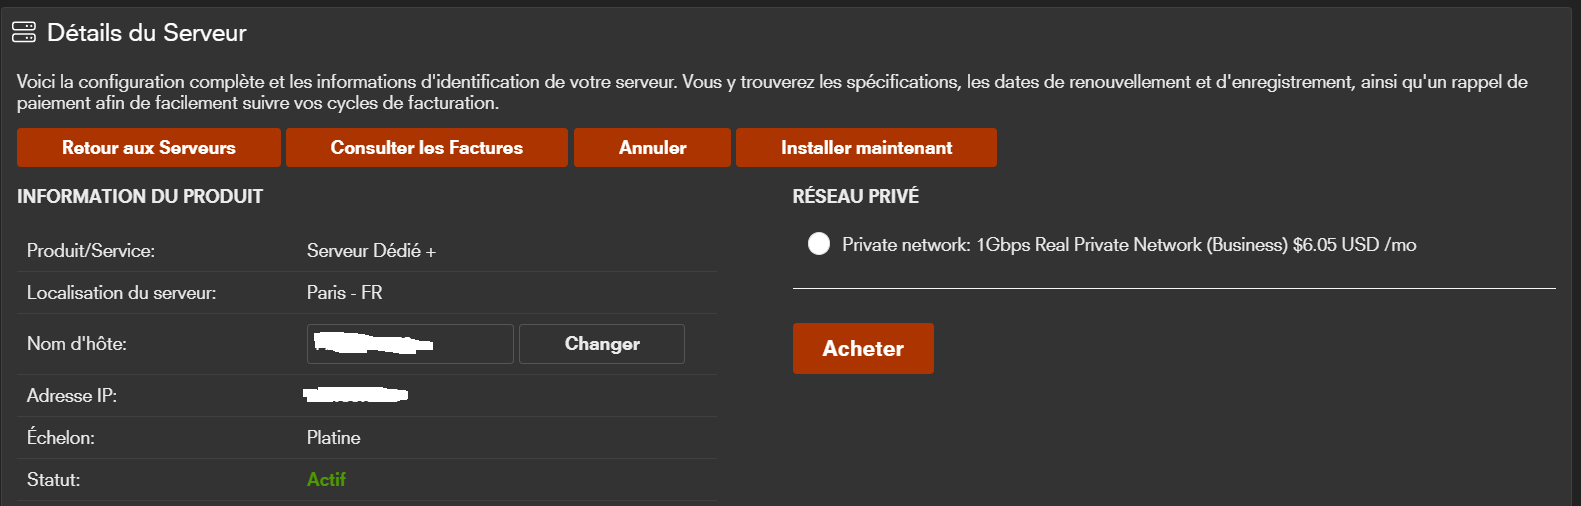
\includegraphics[width=0.9\textwidth]{figures/captures/dep_serveur_details.png}
    \caption{Fiche du serveur dans le panneau OneProvider}
    \label{fig:dep_serveur_details}
\end{figure}

\begin{figure}[H]
    \centering
    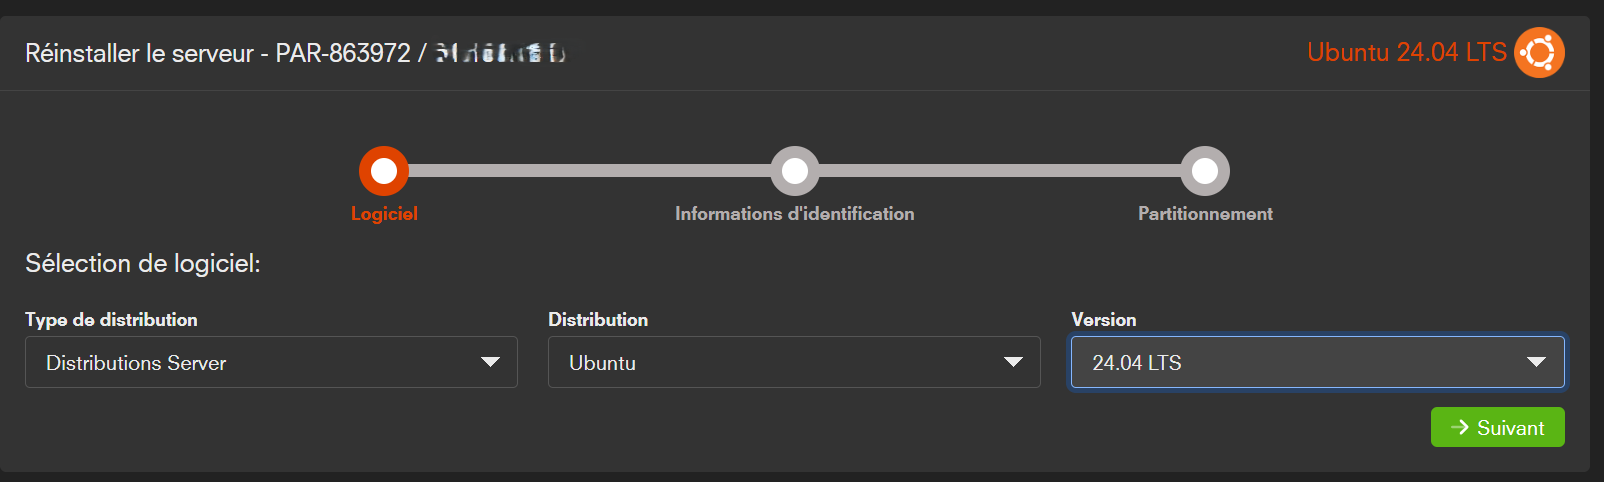
\includegraphics[width=0.9\textwidth]{figures/captures/dep_install_os.png}
    \caption{Réinstallation du serveur, étape 1 : choix d'Ubuntu 24.04 LTS}
    \label{fig:dep_install_os}
\end{figure}

\begin{figure}[H]
    \centering
    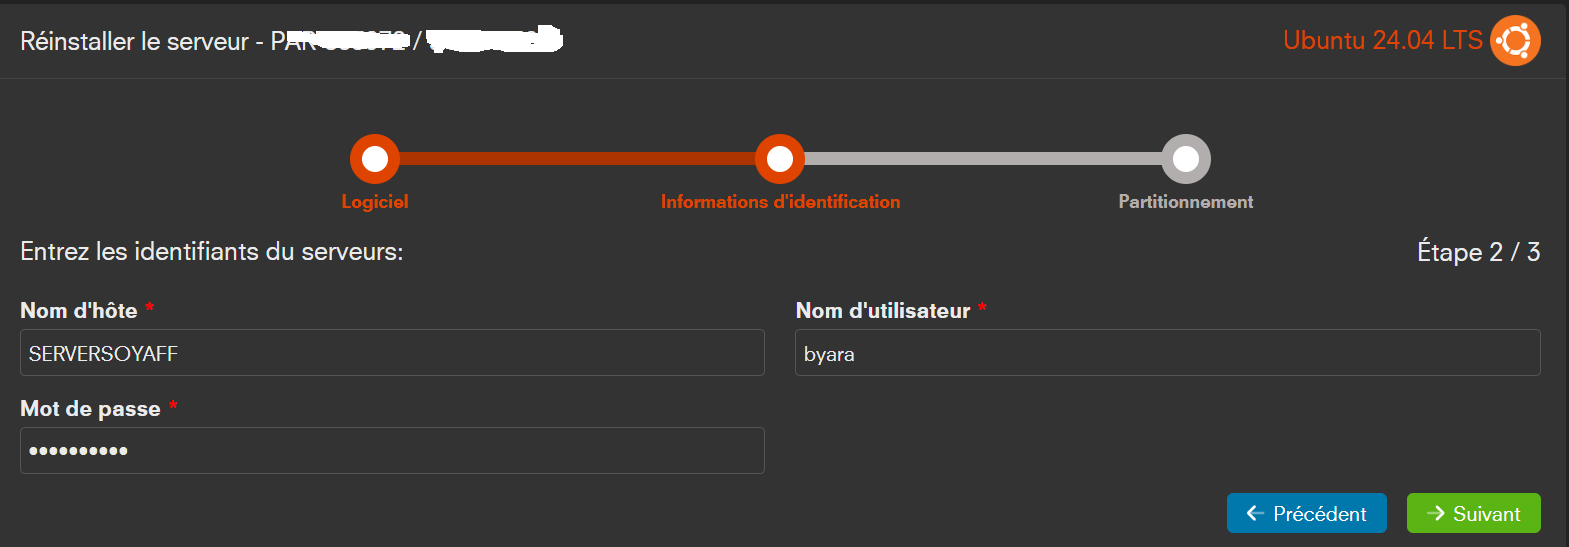
\includegraphics[width=0.9\textwidth]{figures/captures/dep_install_id.png}
    \caption{Réinstallation du serveur, étape 2 : nom d'hôte et compte d'administration}
    \label{fig:dep_install_id}
\end{figure}

\section{Préparation du système}

Après installation, le système a été mis à jour, le pare-feu configuré (Figure~\ref{fig:ops_ufw}), puis Docker installé par le script officiel. Le service Docker est configuré pour attendre le montage du disque qui porte ses données.

\begin{figure}[H]
    \centering
    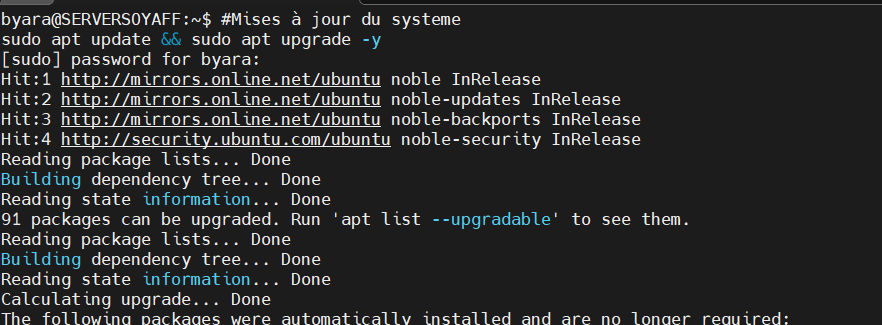
\includegraphics[width=0.8\textwidth]{figures/captures/dep_apt.png}
    \caption{Mise à jour du système}
    \label{fig:dep_apt}
\end{figure}

\begin{figure}[H]
    \centering
    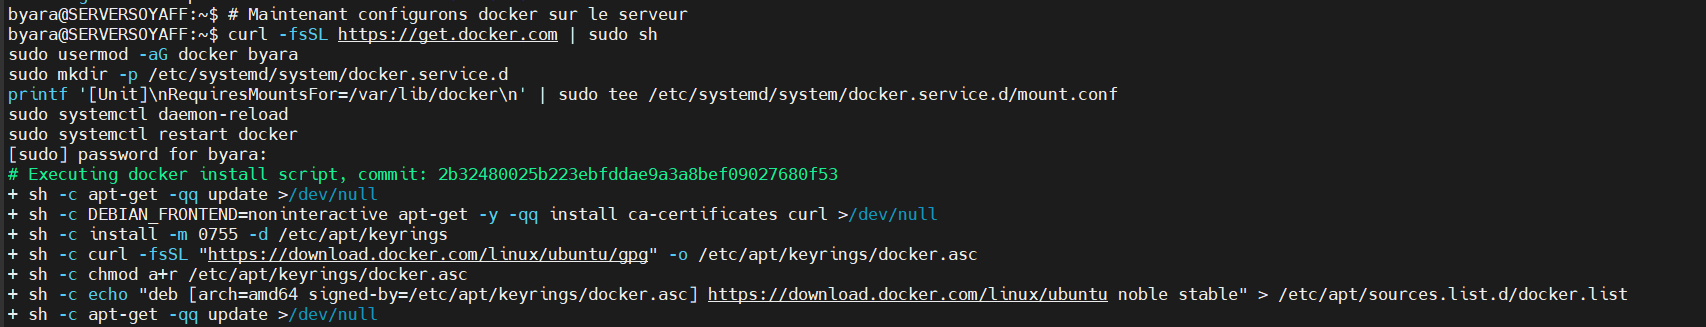
\includegraphics[width=\textwidth]{figures/captures/dep_docker.png}
    \caption{Installation de Docker et dépendance au montage de \texttt{/var/lib/docker}}
    \label{fig:dep_docker}
\end{figure}

\section{Déploiement de la pile IA/ETL}

Le pipeline de \texttt{assistant-soyaff} déploie la pile IA/ETL sur le serveur (\S\ref{sec:devops_cicd}). La Figure~\ref{fig:dep_deploy_ia_ps} montre l'état des conteneurs à l'issue d'un déploiement, et la Figure~\ref{fig:dep_arbo_detail} l'arborescence détaillée du dépôt sur le serveur.

\begin{figure}[H]
    \centering
    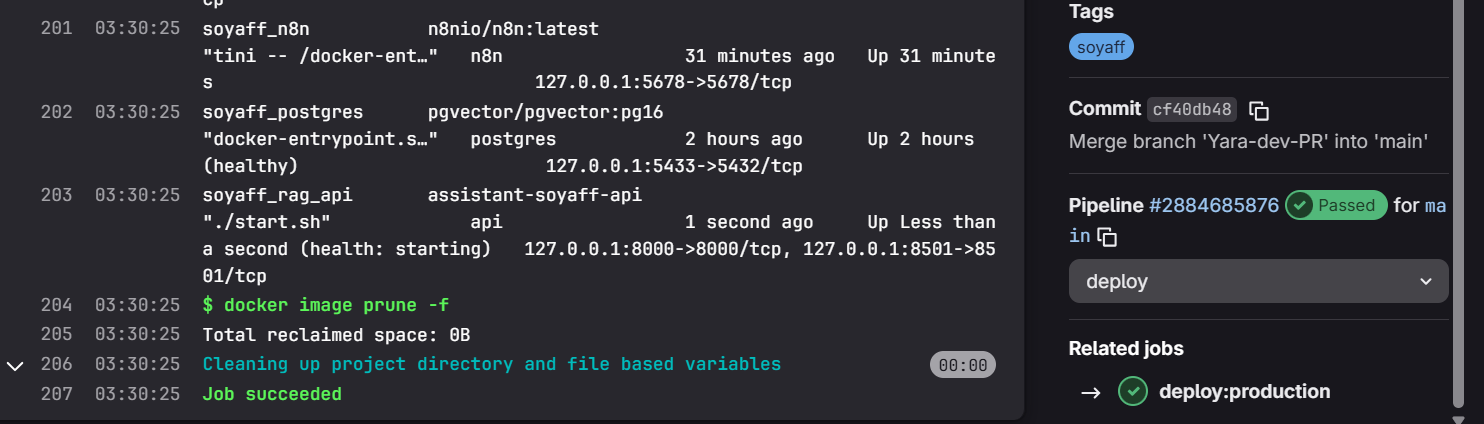
\includegraphics[width=0.85\textwidth]{figures/captures/dep_deploy_ia_ps.png}
    \caption{État des conteneurs de la pile IA/ETL en fin de déploiement}
    \label{fig:dep_deploy_ia_ps}
\end{figure}

\begin{figure}[H]
    \centering
    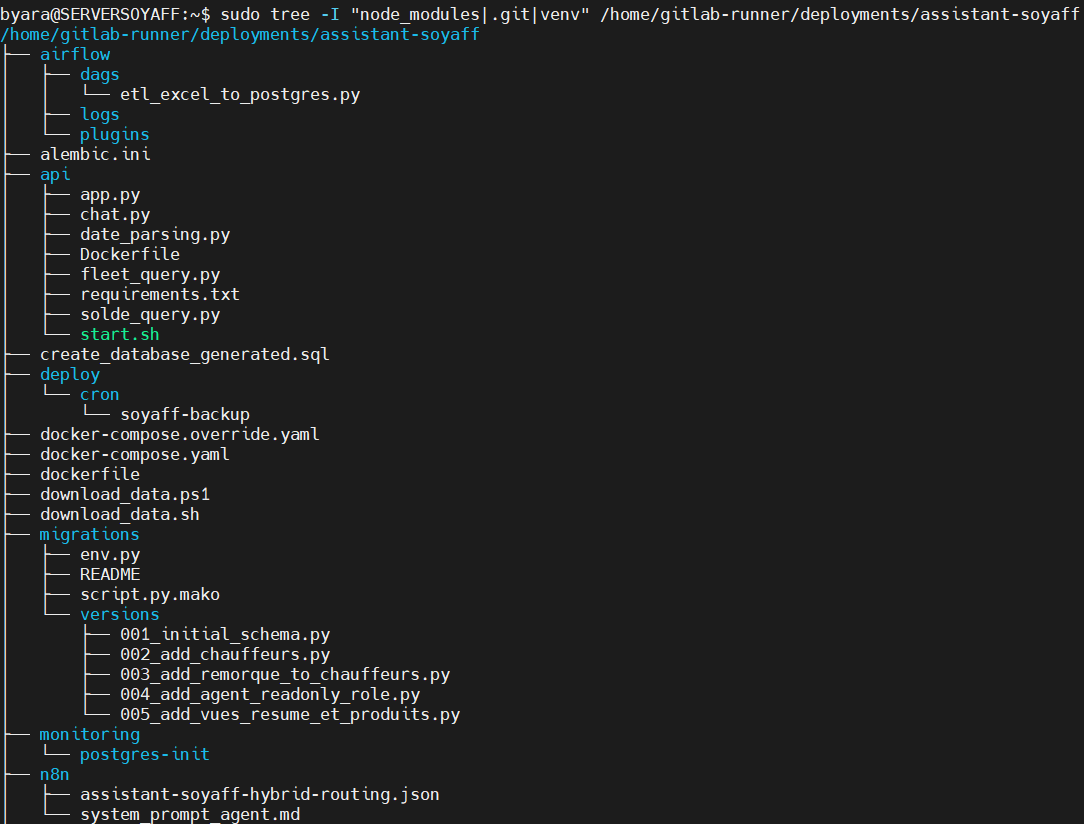
\includegraphics[width=0.75\textwidth]{figures/captures/dep_arbo_detail.png}
    \caption{Arborescence détaillée du dépôt \texttt{assistant-soyaff} sur le serveur}
    \label{fig:dep_arbo_detail}
\end{figure}

Les secrets (mots de passe de la base, clés d'API, jeton du bot Telegram) ne figurent dans aucun dépôt. Ils sont stockés dans les variables protégées de GitLab ; le job de déploiement génère le fichier \texttt{.env} du serveur à partir d'elles, à chaque exécution.

\section{Environnement de développement}

Avant chaque fusion sur \texttt{main}, les services sont exécutés sur le poste de développement avec les mêmes fichiers \texttt{docker compose} qu'en production (Figure~\ref{fig:dep_dev_local}).

\begin{figure}[H]
    \centering
    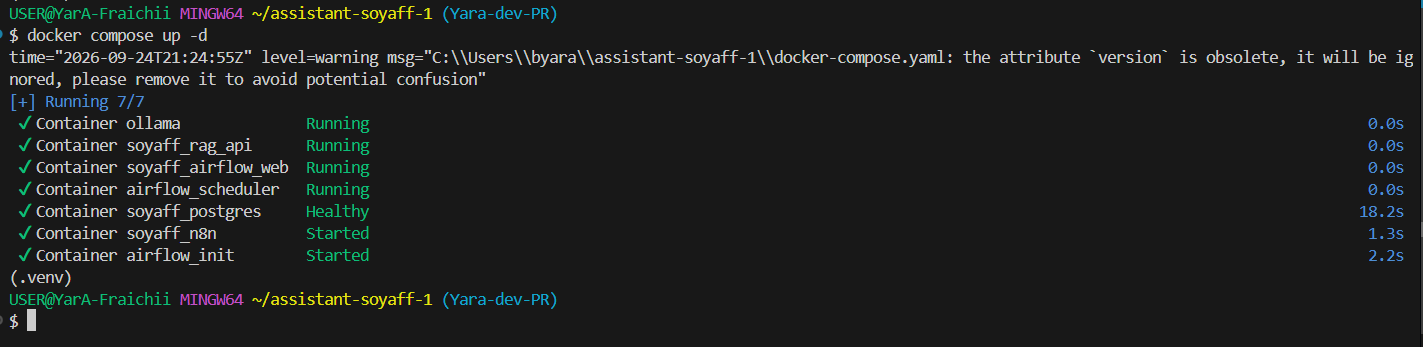
\includegraphics[width=\textwidth]{figures/captures/dep_dev_local.png}
    \caption{Démarrage de la pile IA/ETL sur le poste de développement}
    \label{fig:dep_dev_local}
\end{figure}

\section{Relevé des versions}

Les versions du Tableau~\ref{tab:env_versions} ont été relevées sur le serveur par les commandes suivantes.

\begin{lstlisting}[language=bash, basicstyle=\ttfamily\footnotesize, breaklines=true, showstringspaces=false]
lsb_release -ds; lscpu | grep -E "Model name|^CPU\(s\)"; free -h; df -h /
docker --version; docker compose version
docker exec soyaff_rag_api python --version
docker exec soyaff_postgres psql -U "$POSTGRES_USER" -d "$POSTGRES_DB" \
  -tAc "SELECT version();" \
  -tAc "SELECT extversion FROM pg_extension WHERE extname='vector';"
docker exec airflow_scheduler airflow version
docker exec ollama ollama --version; docker exec ollama ollama list
docker exec soyaff_n8n n8n --version
docker exec soyaff_backend node --version
\end{lstlisting}

\section{Sauvegarde planifiée}

\begin{sloppypar}
La sauvegarde (\S\ref{sec:devops_securite}) est déclarée dans le fichier versionné \texttt{deploy/cron/soyaff-backup}, installé dans \texttt{/etc/cron.d/}. Ses deux tâches actives sont les suivantes.
\end{sloppypar}

\begin{lstlisting}[basicstyle=\ttfamily\footnotesize, breaklines=true, showstringspaces=false]
# Sauvegarde quotidienne a 02:30 (archive locale + copie hors site)
30 2 * * * gitlab-runner cd $DEPLOY_PATH && scripts/backup_db.sh >> /var/log/soyaff/backup.log 2>&1
# Restauration d'essai chaque dimanche a 04:00, dans une base jetable
0 4 * * 0 gitlab-runner cd $DEPLOY_PATH && scripts/restore_db.sh --latest --drop-after >> /var/log/soyaff/restore-drill.log 2>&1
\end{lstlisting}


% ===== INDEX =====
\printindex

% ===== TABLE DES MATIÈRES DÉTAILLÉE (en fin de document) =====
\tableofcontents

\end{document}